%!TEX root = skripsi.tex
%
% Halaman Abstract
%
% @author  Andreas Febrian
% @version 1.00
%

	\chapter*{ABSTRACT}

\vspace*{0.2cm}

\noindent \begin{tabular}{l l p{11.0cm}}
	Name&: & \penulis \\
	Program&: & \programEng \\
	Title&: & \judulInggris \\
\end{tabular} \\ 

\vspace*{0.5cm}

\noindent 
Many of Moslems want to recite \quran. Unfortunatelly, someone who is reciting \quran~needs a partner to help evaluating the recitation. To help that process, this research develops a speech recognition system that is able to automatically evaluate \quran~recitation. The system uses mel frequency cepstral coefficient (MFCC) and shifted delta cepstral coefficient (SDCC) feature, and uses support vector machine (SVM) and Gaussian mixture model (GMM) classification method. The experiment is applied to every ayah in juz 30 of \quran, and gives a result that the best combination to use in the system is SDCC feature with GMM classification method. \\

% \quran~adalah kitab suci bagi umat Muslim. Di dalam \quran~terkandung berbagai macam hakikat kehidupan. Banyak umat Muslim yang ingin belajar membaca \quran~serta menghafalkannya. Orang yang belajar membaca atau menghafalkan \quran~membutuhkan rekan yang mengerti cara membacanya, agar dapat membantu mengevaluasi bacaan \quran. Namun rekan tersebut tidak setiap waktu dapat membantu mengevaluasi. Oleh karena itu, penelitian ini dilakukan dalam rangka membangun sistem pengenalan suara yang mampu mengevaluasi pembacaan \quran~secara otomatis, guna membantu proses evaluasi tersebut. Sistem yang dikembangkan dalam penelitian ini mengekstrak fitur \f{mel frequency cepstral coefficient} (MFCC) dan \f{shifted delta cepstral coefficient} (SDCC) dari audio. Fitur tersebut diklasifikasi menggunakan metode klasifikasi \f{support vector machine} (SVM) dan \f{Gaussian mixture model} GMM. Eksperimen dilakukan terhadap ayat-ayat di juz 30 \quran. Hasil eksperimen dalam penelitian ini menunjukkan bahwa kombinasi yang paling tepat untuk digunakan dalam sistem ini adalah penggunaan fitur SDCC dan metode klasifikasi GMM. \\

% \\ Quran is a holy book for Moslems. It contains much nature in this life. Therefore many of Moslems wants to memorize quran. Quran is originally delivered in Arabic, and it is memorized in Arabic also. The are some ways to memorize quran. One of them is to get help with the second person for heeding the recitation. Whenever the recitation of the first person is wrong, then the second person gives a sign to the first person. Unfortunatelly it cannot be done if there is no second person. Another way is to recite some ayahs, then match them to the original text in quran. That way may slow down memorizing process and also it gives a chance to the reciter to see the next part of quran that should not be seen by him. To make the memorizing process more practical, then a computer system that can cover the second person to match quran recitation to the original quran text, is developed. This system uses Automatic Speech Recognition (ASR).

\vspace*{0.2cm}

\noindent Keywords: \\ 
\noindent Quran, evaluation, speech recognition system, MFCC, SDCC, SVM, GMM \\

\newpage%!TEX root = skripsi.tex
%
% Halaman Abstrak
%
% @author  Andreas Febrian
% @version 1.00
%

\chapter*{Abstrak}

\vspace*{0.2cm}

\noindent \begin{tabular}{l l p{10cm}}
	Nama&: & \penulis \\
	Program Studi&: & \program \\
	Judul&: & \judul \\
\end{tabular} \\ 

\vspace*{0.5cm}

\noindent
Banyak umat Muslim yang ingin menghafalkan \quran. Namun orang yang menghafalkan \quran~membutuhkan rekan untuk membantu mengevaluasi hafalannya. Untuk membantu proses tersebut, penelitian ini mengembangkan sistem pengenalan suara yang mampu mengevaluasi pembacaan \quran~secara otomatis. Sistem tersebut menggunakan fitur \f{mel frequency cepstral coefficient} (MFCC) dan \f{shifted delta cepstral coefficient} (SDCC), serta menggunakan metode klasifikasi \f{support vector machine} (SVM) dan \f{Gaussian mixture model} (GMM). Eksperimen dalam penelitian ini dilakukan terhadap setiap ayat di juz 30 \quran, dan memberikan hasil bahwa kombinasi yang paling tepat untuk digunakan dalam sistem tersebut adalah fitur SDCC dengan metode klasifikasi GMM. \\

% \quran~adalah kitab suci bagi umat Muslim yang diturunkan dalam Bahasa Arab. Di dalam \quran~terkandung berbagai macam hakikat kehidupan. Banyak umat Muslim yang ingin belajar membaca \quran~serta menghafalkan \quran. Orang yang baru belajar membaca \quran~atau orang yang sedang menghafalkannya membutuhkan rekan yang mengerti cara membaca \quran. Peran rekan tersebut adalah untuk mengevaluasi bacaan orang yang sedang belajar \quran~atau yang sedang menghafalkan \quran. Namun rekan untuk mengevaluasi tidak setiap saat ada. Oleh karena itu, penelitian ini dilakukan dalam rangka membangun sistem pengenalan suara yang mampu mengevaluasi pembacaan \quran~secara otomatis, guna membantu proses evaluasi tersebut. Sistem yang dikembangkan dalam penelitian ini mengekstrak fitur MFCC dan SDCC dari audio. Fitur tersebut diklasifikasi menggunakan metode klasifikasi SVM dan GMM. Eksperimen dilakukan terhadap ayat-ayat di juz 30 \quran. Hasil eksperimen menunjukkan bahwa kombinasi yang paling tepat untuk digunakan dalam sistem ini adalah penggunaan fitur SDCC dan metode klasifikasi GMM. \\

% \\ \quran~adalah kitab suci bagi umat islam. Di dalamnya terkandung berbagai macam hakikat kehidupan. Oleh karena itu, banyak umat islam yang ingin menghafalkan \quran. \quran~diturunkan dalam Bahasa Arab, dan dalam Bahasa Arab pula dihafalkan. Cara menghafalkan \quran~ada berbagai macam. Salah satunya adalah dengan meminta bantuan orang kedua untuk menyimak hafalannya. Ketika ada bacaan yang salah dari orang pertama, maka orang kedua mengingatkan atau memberi tanda kepada orang pertama. Namun hal itu tidak dapat dilakukan jika tidak ada orang kedua. Cara lain adalah dengan membaca beberapa ayat, lalu mencocokkan yang dibaca dengan yang ada di \quran. Hal itu selain menghambat proses menghafal karena harus sering melihat ke teks \quran, juga memberi peluang orang yang menghafal melihat bagian selanjutnya yang seharusnya tidak boleh dia lihat. Kemudian untuk membuat proses menghafal lebih praktis, maka dikembangkan sistem komputer yang mampu menggantikan peran sebagai orang kedua, yaitu mencocokkan bacaan yang dibaca oleh penghafal dengan teks \quran~yang benar. Sistem ini menggunakan Pengenalan Suara Otomatis (PSO), atau dalam Bahasa Inggris dikenal sebagai {\em Automatic Speech Recognition} (ASR).



\vspace*{0.2cm}

\noindent Kata Kunci: \\ 
\noindent \quran, evaluasi, sistem pengenalan suara, MFCC, SDCC, SVM, GMM \\ 

\newpage%!TEX root = skripsi.tex
%-----------------------------------------------------------------------------%
\chapter{\babSatu}
%-----------------------------------------------------------------------------%


%-----------------------------------------------------------------------------%
\section{Latar Belakang}
%-----------------------------------------------------------------------------%
	\quran~adalah kitab suci bagi umat Islam yang diturunkan dalam Bahasa Arab. Di dalamnya terkandung segala macam hakikat kehidupan. Walaupun banyak terjemahan \quran~dalam berbagai bahasa, namun keaslian \quran~dalam Bahasa Arab tetap dijaga. Salah satunya adalah karena makna \quran~yang begitu luas, sehingga tidak ada padanan kata yang mampu menerjemahkan bahasa \quran~secara sempurna. Bahkan dalam bahasa aslinya pun, makna yang dapat diambil dari satu ayat \quran~bisa bervariasi. Oleh karena itu, banyak umat Islam yang ingin menghafalkan \quran~dalam Bahasa Arab.
	
	Ada berbagai macam cara dalam menghafal Al-Qur'an. Salah satunya adalah dengan cara berpasangan. Orang pertama membacakan \quran~yang dihafalnya dan orang kedua mendengarkannya. Tugas orang kedua cukup sederhana, yaitu mendengarkan bacaan orang pertama, lalu mengevaluasi kebenaran pelafalan bacaannya. Namun cara seperti ini tidak dapat dilakukan jika tidak ada orang kedua atau orang kedua tidak mengerti bacaan yang benar. Alternatif solusi dari masalah tersebut adalah dengan memanfaatkan teknologi yang ada saat ini.
	
	Teknologi Sains dan Komputasi yang berkembang beberapa tahun terakhir mampu mengakomodir sebagian besar kebutuhan manusia sehari-hari. Salah satunya adalah sistem Pengenalan Suara Otomatis, atau lebih umum dikenal dengan nama \textit{Automatic Speech Recognition} (ASR).  ASR adalah proses yang dilakukan komputer untuk menafsirkan ucapan manusia \citep{forsberg2003speech}. Menurut \cite{IJIR37}, ASR adalah teknologi yang memungkinkan sebuah komputer untuk mengidentifikasi kata-kata yang diucapkan oleh manusia dan mengubahnya menjadi teks tertulis.
	
	Melihat kendala menghafal \quran~di atas dan teknologi yang berkembang saat ini, maka dimungkinkan untuk membuat alternatif solusi. Sistem ASR dapat dikembangkan untuk mengenali pelafalan bacaan Al-Qur'an, sehingga diharapkan akan ada peran komputer dalam membantu proses menghafal. Tugas komputer sebagai pengganti orang yang menyimak hafalan, yaitu mengevaluasi pelafalan bacaan \quran~oleh penghafal dalam bentuk suara digital dengan suara pelafalan bacaan \quran~yang benar.
	
	Hal lain yang menjadi dasar dilakukannya penelitian ini adalah kedudukan \quran~yang istimewa. Walaupun naskah asli \quran~dalam Bahasa Arab, namun gaya bahasa \quran~tidak seperti gaya bahasa yang digunakan masyarakat Arab pada umumnya. Begitu pula cara membaca \quran~yang memiliki aturan-aturan tersendiri. Aturan-aturan tersebut dinamakan \textit{tajwid}, di mana dalam Bahasa Arab sehari-hari tidak dijumpai adanya \textit{tajwid}. Penjelasan lebih lanjut mengenai \textit{tajwid} akan dijelaskan di Bab \ref{bacaan quran}. Hal ini mengakibatkan perlakuan dalam mengolah audio pelafalan bacaan \quran~menjadi berbeda dengan pengolahan sistem ASR Bahasa Arab. Maka dengan keistimewaan ini dimungkinkan adanya hal-hal menarik yang dapat ditemukan selama proses penelitian.

%-----------------------------------------------------------------------------%
\section{Perumusan Masalah}
%-----------------------------------------------------------------------------%
Berdasarkan latar belakang permasalahan yang ada, terdapat tiga pertanyaan yang akan diselesaikan dalam penelitian ini.
\begin{enumerate}
	\item Bagaimana membangun sistem komputasi yang dapat mengenali kebenaran pelafalan bacaan Al-Qur'an?
	\item Metode seperti apa yang menghasilkan akurasi terbaik dari sistem yang dibangun?
	\item Apa saja fakta-fakta baru yang dapat diambil dari proses pengolahan audio yang berupa bacaan Al-Qur'an?
\end{enumerate}

%-----------------------------------------------------------------------------%
\section{Tujuan dan Manfaat Penelitian}
%-----------------------------------------------------------------------------%
Penelitian ini bertujuan untuk membangun sistem yang mampu mengenali kebenaran pelafalan bacaan Al-Qur'an. Penelitian ini mencakup rancangan sistem sampai dengan implementasi metode yang menghasilkan akurasi terbaik. Diharapkan dengan adanya teknologi ini, komputer akan mampu melakukan evaluasi pelafalan bacaan \quran~kapan pun dan di mana pun. Selain itu, penelitian ini juga bertujuan untuk mencari hal-hal menarik dalam dunia \textit{speech recognition} di mana domain penelitiannya berupa ayat-ayat Al-Qur'an.

Manfaat dari penelitian ini adalah menghasilkan rancangan suatu sistem dan metode yang dapat dibungkus menjadi sebuah \textit{software} untuk membantu pengguna dalam memantau hafalan Al-Qur'an. Selama ini, penghafalan bacaan \quran~memerlukan rekan untuk menyimak dan memperbaiki bacaan hafalan tersebut. Namun jika ada \textit{software} yang dapat membantu menjalankan tugas tersebut, tentunya proses menghafal \quran~akan sangat terbantu dari segi evaluasinya. Penghafal tidak perlu lagi berulang-kali melihat ke teks \quran~untuk memeriksa apakah yang dilafalkan sudah benar atau belum. Kemudian metode evaluasi pelafalan bacaan \quran~dapat digunakan sebagai metode pencarian dalam Al-Qur'an. Caranya adalah dengan mencocokkan ayat demi ayat hingga ditemukan ayat yang cocok. Lebih jauh lagi, penelitian ini juga dapat dimanfaatkan sebagai bahan acuan untuk penelitian selanjutnya yang terkait dengan bidang dan domain yang sama.


%-----------------------------------------------------------------------------%
\section{Metodologi Penelitian}
%-----------------------------------------------------------------------------%
Berikut ini adalah metode penelitian yang \saya~lakukan.
\begin{enumerate}
	\item Studi Literatur\\
	Pada tahapan ini \saya~mempelajari literatur yang dapat mendukung terselesaikannya penelitian ini. Literatur yang digunakan bersumber dari makalah, jurnal, buku, dan  artikel yang ada di internet. Bahan-bahan yang \saya~jadikan literatur semuanya memiliki kaitan dengan topik ASR, audio, maupun Al-Qur'an.
	
	\item Perumusan Masalah \\
	Pada tahapan ini \saya~merumuskan permasalahan yang akan dijawab melalui penelitian ini. Rumusan masalah ini didapatkan setelah \saya~mempelajari literatur yang ada dan penerapannya dalam konteks pelafalan bacaan Al-Qur'an. 
	
	\item Perancangan Sistem \\
	Pada tahapan ini, \saya~merancang suatu sistem yang dapat menjadi pedoman \saya~dalam melakukan penelitian ini. Tahapan ini dilakukan untuk memudahkan \saya~dalam melakukan eksperimen dan usaha menyelesaikan masalah pada penelitian ini.
		
	\item Eksperimen \\
	Tahap ini merupakan bagian inti dari penelitian. Dengan melakukan serangkaian eksperimen, \saya~berusaha memperoleh jawaban dari pertanyaan-pertanyaan yang ada pada bagian perumusan masalah.
	
	\item Analisis Hasil \\
	Pada tahapan ini \saya~melakukan analisis dari hasil eksperimen pada tahap sebelumnya.
		
	\item Penarikan Kesimpulan \\
	Tahap ini merupakan tahap terakhir dari penelitian, di mana \saya~memberikan kesimpulan dari hasil analisis di tahap sebelumnya. Selain itu \saya~juga memberikan saran sebagai bahan pertimbangan untuk penelitian selanjutnya.
\end{enumerate}

%-----------------------------------------------------------------------------%
\section{Ruang Lingkup Penelitian}
Pada penelitian ini terdapat beberapa batasan yang \saya~tentukan, yaitu sebagai berikut:
\begin{enumerate}
\item{\bf Batasan Sistem}\\
Sistem melakukan pengenalan per satu ayat secara utuh, bukan potongan ayat, dan hanya melibatkan ayat-ayat yang terdapat di juz 30 Al-Qur'an. Hal ini dikarenakan ayat-ayat dalam juz 30 merupakan ayat yang berdurasi singkat, dengan rata-rata durasi 5,5109 detik. Audio dengan durasi itu dapat langsung diolah oleh sistem tanpa perlu disegmentasi terlebih dahulu.
	
\item{\bf Kriteria Data}\\
Data yang digunakan dalam penelitian ini merupakan audio bebas \textit{noise}. Untuk memastikan data audio tersebut bebas \f{noise} dan layak digunakan dalam penelitian, maka data tersebut perlu diuji secara manual, dengan cara didengarkan langsung. Penelitian ini hanya berfokus pada metode, tidak termasuk proses pembersihan audio dari \f{noise}. Sampel yang digunakan merupakan sampel yang sesuai standar, yaitu sampel dari orang yang cara melafalkan bacaan Al-Qur'annya sudah benar. Karena jika sampel merupakan bacaan yang kurang benar atau tidak sesuai standar, maka hal tersebut akan membuat hasil eksperimen sulit untuk dianalisis dengan tepat. Bacaan standar diperoleh dari para pembaca \quran~tingkat internasional, yang akan dijelaskan lebih lanjut cara memperolehnya di Bab \ref{pengambilan data}.
	
\item{\bf Penerapan Metode}\\
Penelitian ini difokuskan pada kombinasi pemilihan fitur dan metode klasifikasi terbaik. Metode klasifikasi yang digunakan merupakan metode klasifikasi umum, dengan parameter yang akan dibahas detil pada Bab \ref{eksperimen}, dan tidak sampai pada optimasi metode klasifikasi untuk menghasilkan akurasi terbaik. Optimasi dapat dilakukan di penelitian selanjutnya, jika arsitektur sistem dan fitur yang digunakan dengan metode klasifikasi tersebut sudah menghasilkan akurasi yang baik.
	
\item{\bf Aplikasi}\\
Penelitian ini hanya dibataskan sampai metode, tidak sampai ke tahap pembuatan aplikasi. Karena keterbatasan waktu penelitian, maka tidak dimungkinkan penelitian ini dilakukan sampai ke tahap pembuatan aplikasi. Pembuatan aplikasi dapat dilakukan oleh pihak ketiga setelah metode yang dipilih untuk pengenalan pelafalan bacaan \quran~sudah menghasilkan akurasi yang baik.
\end{enumerate}

%-----------------------------------------------------------------------------%

%-----------------------------------------------------------------------------%
\section{Sistematika Penulisan}
%-----------------------------------------------------------------------------%
Sistematika penulisan yang ada dalam laporan penelitian ini sebagai berikut:
\begin{itemize}

	\item Bab 2 \babDua \\
	Pada bab ini \saya~menjelaskan teori-teori terkait topik yang \saya~dapatkan melalui studi literatur untuk melakukan penelitian ini.
		
	\item Bab 3 \babTiga \\
	Pada bab ini \saya~menjelaskan rancangan dari sistem yang akan \saya~kembangkan dalam penelitian ini.
		
	\item Bab 4 \babEmpat \\
	Pada bab ini \saya~menjelaskan proses implementasi sistem berdasarkan rancangan sistem yang sudah dilakukan pada bab sebelumnya, sampai dengan tahap pengujian.
		
	\item Bab 5 \babLima \\
	Pada bab ini \saya~menjelaskan mengenai analisis dari hasil pengujian sistem yang sudah \saya~kerjakan pada tahap sebelumnya. Pada bab ini juga dipaparkan hal-hal menarik yang ditemukan selama penelitian.
	
	\item Bab 6 \babEnam \\
	Pada bab ini \saya~memberikan kesimpulan berdasarkan hasil pengujian dan analisis sistem yang sudah dilakukan pada bab sebelumnya. Selain itu terdapat pula saran-saran untuk penelitian selanjutnya.
	
\end{itemize}%!TEX root = skripsi.tex
%-----------------------------------------------------------------------------%
\chapter{\babDua}
%-----------------------------------------------------------------------------%

%-----------------------------------------------------------------------------%
\section{Bacaan Al-Qur'an} \label{bacaan quran}
%-----------------------------------------------------------------------------%
\quran~adalah kitab suci umat muslim yang istimewa dan memiliki banyak nama. Dalam bukunya yang berjudul \f{Holy Quran}, \cite{ali2011holy} menjelaskan bahwa nama \f{Al-Qur'an} (\<القرآن>) adalah nama asli dari kitab suci ini. Nama ini disebut beberapa kali di dalam \quran~itu sendiri. Kata \f{Al-Qur'an} berasal dari kata dasar \f{qara'a} (\<قرأ>) yang berarti membaca. Alasan kenapa dinamakan \quran~adalah karena di dalamnya berisi bacaan-bacaan pelajaran religi yang baik dan karena kitab ini diturunkan untuk dibaca. Adapun nama lain dari \quran~adalah \f{Al-Kitab} (\<الكتاب>) yang berarti tulisan, \f{Al-Furqon} (\<الفرقان>) yang berarti pembeda, dan \f{Al-Dzikr} (\<الذكر>) yang berarti pengingat.

\quran~diturunkan dalam Bahasa Arab, begitu pula cara membacanya atau pun menghafalkannya. Cara membaca teks \quran~mirip dengan cara membaca teks bahasa Arab, namun ada kaidah-kaidah tambahan yang harus diikuti, yang disebut \f{tajwid}. Karena itu bacaan \quran~menjadi istimewa dan berbeda dengan ucapan Bahasa Arab sehari-hari. Adapun orang yang membaca \quran~disebut \f{qari} dan rekaman bacaan \quran~dari qari disebut \f{murotal}.

Satu \quran~dibagi sama rata ke dalam 30 bagian, yang masing-masing disebut dengan \f{juz}. Dalam \quran~terdapat 114 \f{surat}, di mana setiap surat terdiri dari beberapa \f{ayat}, bervariasi mulai dari 3 ayat sampai 286 ayat. Total seluruh ayat dalam \quran~ada sebanyak 6,236 ayat. Ayat-ayat \quran~tidak seluruhnya unik, karena ada beberapa pasang ayat yang sama dan ada beberapa pasang ayat yang mirip. Hal ini bisa dideteksi menggunakan algoritma yang akan dijelaskan di Bab \ref{lcs}.

%-----------------------------------------------------------------------------%
\section{Pengenalan Suara Otomatis}
%-----------------------------------------------------------------------------%
Pengenalan Suara Otomatis atau yang lebih umum dikenal dengan \f{Automatic Speech Recognition} (ASR) memiliki beberapa definisi dari sumber yang berbeda. Menurut \cite{forsberg2003speech}, ASR adalah proses yang dilakukan komputer untuk menafsirkan ucapan manusia. Definisi lebih teknis diberikan oleh \cite{Jurafsky:2009:SLP:1214993}, yaitu ASR adalah sebuah sistem untuk memetakan sinyal akustik ke dalam untaian kata. Selain definisi-definisi yang telah disebutkan sebelumnya, \cite{chigier1997automatic} menambahkan bahwa ASR merupakan proses komputasi yang bertujuan untuk menangkap sinyal akustik yang merepresentasikan ucapan dan menentukan kata-kata yang diucapkan menggunakan pencocokan pola.

Teknik dalam membangun sistem ASR berbeda-beda, namun secara garis besar ada kesamaan. Sistem pengenalan suara umumnya memiliki sekumpulan model akustik dan bahasa yang direpresentasikan sebagai pola, dan disimpan dalam sebuah basis data komputer. Model-model ini kemudian dibandingkan dengan sinyal yang ditangkap. Untuk sistem ASR yang mengandung sedikit kosakata (kurang dari 50 kata), sebuah model dapat merepresentasikan sebuah kata. Namun untuk kosakata yang lebih dari 50 kata, proses pemodelan dan algoritma pengenalan membutuhkan komputasi yang banyak dan tidak praktis. Oleh karena itu, sistem dengan kosakata yang banyak (lebih dari 1000 kata) membuat sebuah model yang merepresentasikan komponen yang lebih kecil dari kata, sebagai contoh adalah \f{fonem}. Deretan fonem dapat dirangkai untuk menghasilkan sebuah model kata.

\cite{juang2005automatic} dalam artikelnya yang berjudul \f{Automatic Speech Recognition -- A Brief History of the Technology Development} menjelaskan bahwa saat ini teknologi ASR sudah tersedia secara komersial, walaupun hanya mampu menjalankan tugas-tugas yang terbatas. Teknologi ini memungkinkan mesin untuk menanggapi perintah manusia melalui suara dengan baik. Namun teknologi tersebut masih jauh dari kemampuan untuk bercakap-cakap dengan manusia dalam berbagai topik bebas. Perkembangan dalam bidang sains dan teknologi semakin mendorong sistem ASR untuk menjadi sistem yang mampu mengenali dan memahami ucapan manusia dengan baik.

Sejarah singkat mengenai perkembangan ASR dapat dikelompokkan ke dalam beberapa era. Dimulai pada sekitar tahun 1960, di mana pada saat itu telah berhasil dikembangkan teknologi yang mampu mengenali kosakata dalam skala kecil (10 sampai 100 kata). Pengenalan ini dilakukan dengan mengenali kata demi kata secara terpisah berdasarkan sifat-sifat \f{acoustic-phonetic} yang terdapat dalam suara. \f{Acoustic-phonetic} adalah ilmu tentang karakteristik akustik dari suara. Kunci dari keberhasilan teknologi ASR di era ini adalah analisis \f{filter-bank}, metode normalisasi \f{simple time}, dan permulaan dari metodologi \f{dynamic programming} yang canggih. \f{Filter-bank} adalah pembagian sinyal \f{input} $x(n)$ ke dalam himpunan sinyal analisis  $x_1(n), x_2(n), \ldots$, yang masing-masing berkorespondensi terhadap wilayahnya di dalam spektrum $x(n)$.

Sekitar tahun 1970, teknologi yang berkembang mampu untuk mengenali kosakata dalam skala sedang (100 sampai 1000 kata). Kunci perkembangan teknologi di era ini adalah model pengenalan pola (\f{pattern recognition}), permulaan metode \f{Linear Predictive Coding} (LPC) untuk merepresentasikan spektrum, metode \f{pattern clustering} untuk \f{speaker-independent recognizers}, dan permulaan metode \f{dynamic programming} untuk menyelesaikan permasalahan \f{connected word recognition}. Sekitar tahun 1980, teknologi ASR mampu menangani kosakata dalam skala besar (1000 kata atau lebih). Kunci dari keberhasilan di era ini adalah model statistik \f{Hidden Markov Model} (HMM) dan model bahasa \f{stochastic}.

Teknologi semakin maju pada sekitar tahun 1990. Sistem ASR dengan kosakata berskala besar yang lebih canggih dari era sebelumnya telah berhasil dikembangkan pada era ini, dengan adanya \f{continuous speech recognition and understanding}. Adapun keberhasilan teknologi ASR di era ini berkat metode untuk melakukan \f{stochastic language understanding}, pembelajaran statistik dari model akustik dan model bahasa, permulaan \f{finite state transducer framework} (dan juga \f{FSM Library}), serta metode untuk determinasi dan minimalisasi untuk implementasi sistem \f{speech understanding} yang efisien dengan kosakata berskala besar. Akhirnya sekitar tahun 2000, muncul permulaan dari sistem ASR dengan kosakata berskala sangat besar disertai model semantik penuh, terintegrasi dengan sistem sintesis \f{text-to-speech} (TTS), dan \f{multi-modal inputs}.



%-----------------------------------------------------------------------------%
\section{Fitur}
%-----------------------------------------------------------------------------%
Informasi tertentu yang diambil dari data disebut \f{fitur}. Proses pengambilan fitur dari data dinamakan proses \f{ekstraksi fitur}. Dalam sistem ASR, fitur yang populer digunakan antara lain adalah \f{Mel Frequency Cepstral Coefficients} dan \f{Shifted Delta Cepstral Coefficients}.

	\subsection{Mel Frequency Cepstral Coefficients (MFCCs)} \label{teorimfcc}
	\f{Mel frequency cepstral coefficients} (MFCCs) adalah salah satu fitur modern dalam teknologi \f{speech}, yang diperkenalkan oleh \cite{1163420}. Fitur ini sudah banyak digunakan dalam ASR \citep{young2002htk}, verifikasi \f{speaker} \citep{ganchev2005comparative}, dan juga di dalam identifikasi bahasa lisan \citep{yin2006combining}. MFCCs adalah fitur yang berbasis spektrum \f{short-term}. Dalam penelitian tentang \f{speech}, \f{short term} sering dipilih sebagai fitur dengan asumsi bahwa secara statistik sinyal bersifat stasioner dalam periode waktu singkat. Namun jika terlalu singkat, banyaknya sampel tidak akan cukup untuk menghasilkan estimasi spektrum tepat. Umumnya interval waktu untuk sebuah \fr~adalah 20 ms sampai dengan 40 ms \citep{zahra2013unique}.

  \cite{hitungmfcc} menjelaskan secara garis besar cara menghitung nilai MFCCs dari sebuah data audio. Langkah-langkahnya adalah sebagai berikut.
  \begin{enumerate}
    \item Bagi sebuah sinyal ke dalam beberapa \fr~singkat.
    \item Hitung estimasi \f{periodogram} dari \f{power spectrum} pada setiap \fr.
    \item Terapkan \f{mel filter-bank} ke setiap \f{power spectrum}, lalu jumlahkan energi di setiap \f{filter}.
    \item Hitung nilai logaritma dari seluruh energi \f{filter-bank}.
    \item Hitung nilai \f{discrete cosine transform} (DCT) dari logaritma energi \f{filter-bank}.
    \item Pertahankan koefisien ke-2 sampai ke-13 saja dari DCT.
  \end{enumerate}



	\subsection{Shifted Delta Cepstral Coefficients (SDCCs)}  \label{teorisdcc}
  \f{Shifted delta cepstral coefficients (SDCCs)} adalah pengembangan dari MFCCs \citep{torres2002approaches}. Untuk menghitung SDCCs diperlukan nilai MFCCs sebagai salah satu parameter dalam komputasi SDCCs. Vektor fitur SDCCs diperoleh dengan cara menumpuk \f{delta cepstral} yang dihitung dari beberapa \fr. Selain nilai MFCCs, fitur SDCCs membutuhkan 4 parameter tambahan sebagai berikut.
  \begin{enumerate}
    \item N: banyaknya koefisien-koefisien \f{cepstral} yang dihitung pada setiap \fr
    \item \f{d}: waktu untuk \f{advance} dan \f{delay} untuk komputasi \f{delta}
    \item \f{P}: pergeseran waktu antarblok berurutan
    \item \f{k}: banyaknya blok di mana koefisien \f{delta} disambungkan untuk membentuk vektor fitur akhir
  \end{enumerate}
  
  Menurut \cite{zahra2013unique}, ide dari perhitungan ini adalah menghitung jarak antara pasangan N koefisien \f{cepstral} paralel yang dipisahkan oleh waktu \f{advance} dan \f{delay} \f{t}, dilakukan pada \f{k} blok dengan waktu geser \f{P} antarblok yang berurutan. Semua nilai jarak ini kemudian disatukan menjadi sebuah vektor. Langkah ini dilakukan secara iteratif dari awal sampai akhir \fr~pada \f{speech}, sehingga diperoleh kumpulan vektor yang menjadi nilai SDCCs. Gambar \ref{fig:hitungsdcc} mengilustrasikan bagaimana cara menghitung sebuah vektor SDCC.
  \begin{figure}
    \centering
    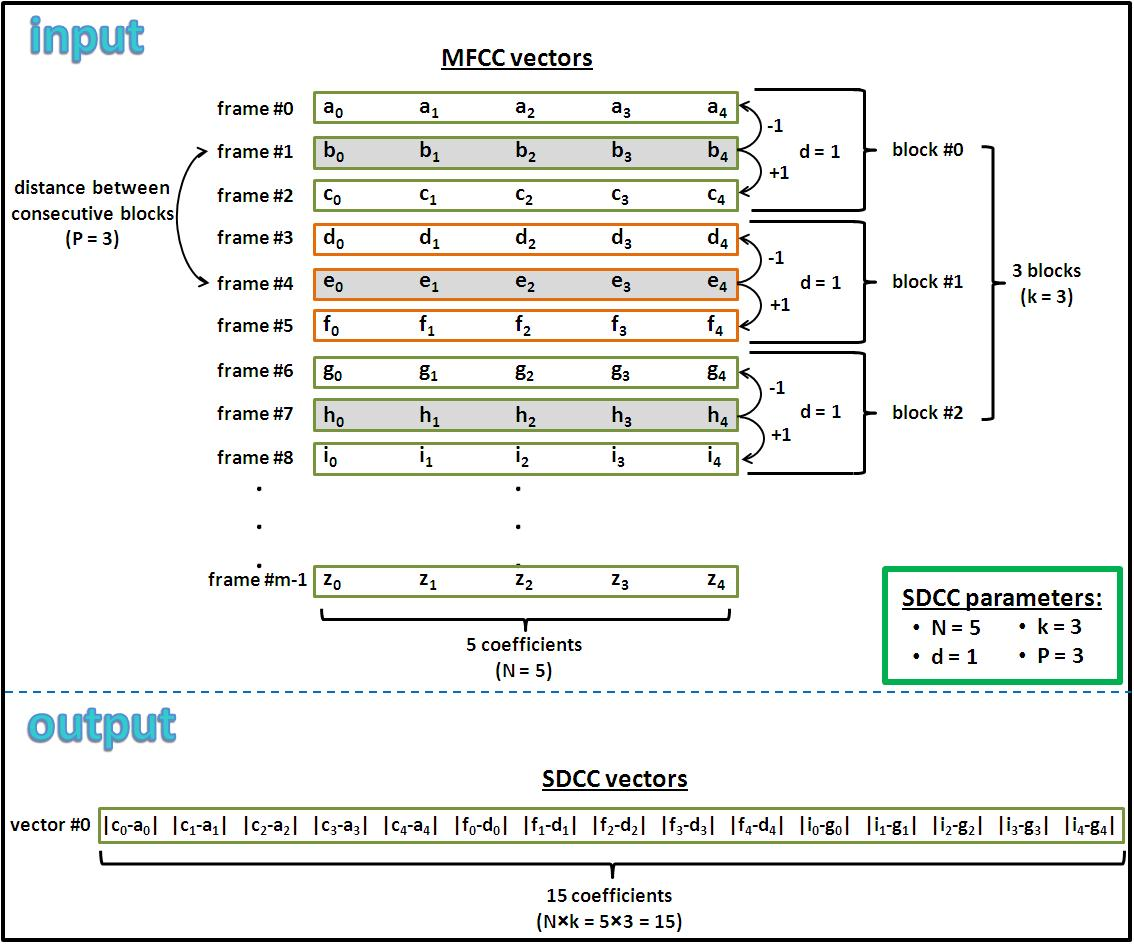
\includegraphics[width=\linewidth]{pics/hitung_sdcc}
    \caption{Contoh Perhitungan Sebuah Vektor SDCC}{Sumber gambar: \cite{zahra2013unique}}
    \label{fig:hitungsdcc}
  \end{figure}



%-----------------------------------------------------------------------------%
\section{Longest Common Subsequence (LCS)}\label{lcs}
%-----------------------------------------------------------------------------%
\cite{Cormen:2009:IAT:1614191} menjelaskan tentang algoritma untuk menyelesaikan permasalahan \f{longest common subsequence} (LCS) dalam bukunya yang berjudul \f{Introduction to Algorithms}. Diberikan sebuah barisan (\f{sequence}) $X=\langle x_1,x_2,...,x_m\rangle$. Barisan $Z=\langle z_1,z_2,...,z_k\rangle$ disebut \textbf{\f{subsequence}} dari $X$ jika terdapat barisan menaik $\langle i_1,i_2,...,i_k\rangle$ berupa indeks dari $X$ sedemikian hingga untuk semua $j=1,2,...,k$, terpenuhi $x_{i_j}=z_j$. Sebagai contoh, $Z=\langle B,C,D,B\rangle$ adalah \f{subsequence} dari $X=\langle A,B,C,B,D,A,B\rangle$ dengan barisan indeks yang berkorespondensi adalah $Z=\langle 2,3,5,7\rangle$.

Diberikan dua buah barisan $X$ dan $Y$. $Z$ disebut \textbf{\f{common subsequence}} dari $X$ dan $Y$ jika Z merupakan \f{subsequence} dari $X$ dan $Y$ sekaligus. Sebagai contoh,  jika $X=\langle A,B,C,B,D,A,B\rangle$, dan $Y=\langle B,D,C,A,B,A\rangle$, barisan $\langle B,C,A\rangle$ adalah \f{common subsequence} dari $X$ dan $Y$ sekaligus. Barisan $\langle B,C,A\rangle$ bukan merupakan \f{common subsequence} terpanjang dari $X$ dan $Y$ karena hanya memiliki panjang 3, sedangkan terdapat barisan $\langle B,C,B,A\rangle$ yang memiliki panjang 4 dan juga merupakan \f{common subsequence} dari $X$ dan $Y$. Karena tidak ada \f{common subsequence} dari $X$ dan $Y$ dengan panjang 5, maka barisan $\langle B,C,B,A\rangle$ merupakan \f{common subsequence} terpanjang atau \textbf{\f{longest common subsequence}} (LCS) dari $X$ dan $Y$.

LCS dapat diselesaikan menggunakan \f{dynamic programming}. Prosedur pada gambar \ref{fig:prosedurlcs} menjelaskan cara untuk menghitung nilai LCS. Prosedur tersebut membutuhkan dua buah barisan sebagai \f{input}, yaitu $X=\langle x_1,x_2,...,x_m\rangle$ dan $Y=\langle y_1,y_2,...,y_n\rangle$, dan memberikan tabel $b$ dan $c$ sebagai \f{output}. Nilai LCS terdapat pada $c[m,n]$.

\begin{figure}
  \centering
  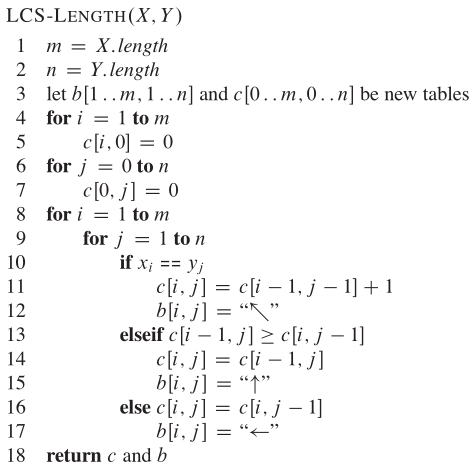
\includegraphics[width=0.7\linewidth]{pics/prosedur_lcs}
  \caption{Prosedur LCS-Length}{Sumber gambar: \cite{Cormen:2009:IAT:1614191}}
  \label{fig:prosedurlcs}
\end{figure}

Gambar \ref{fig:tabellcs} memperlihatkan bagaimana isi tabel yang dihasilkan dari prosedur LCS-Length pada barisan $X=\langle A,B,C,B,D,A,B\rangle$ dan $Y=\langle B,D,C,A,B,A\rangle$.

\begin{figure}
  \centering
  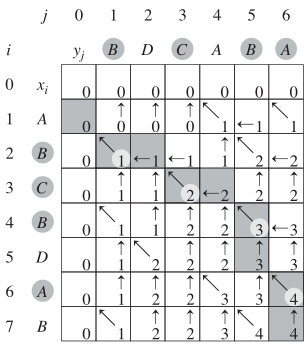
\includegraphics[width=0.55\linewidth]{pics/tabel_lcs}
  \caption{Tabel $c$ dan $b$ yang Dihasilkan oleh Prosedur LCS-Length}{Sumber gambar: \cite{Cormen:2009:IAT:1614191}}
  \label{fig:tabellcs}
\end{figure}


%-----------------------------------------------------------------------------%
\section{Metode \f{Clustering} dan Klasifikasi}
%-----------------------------------------------------------------------------%
Metode \f{clustering} dan klasifikasi adalah dua hal yang mirip. \f{Clustering} mengelompokkan data tanpa diketahui labelnya, sedangkan klasifikasi mengelompokkan data dengan diketahui labelnya.

  %-----------------------------------------------------------------------------%
  \subsection{K-Means Clustering}
  %-----------------------------------------------------------------------------%
  \f{Clustering} adalah proses mengelompokkan data menurut kemiripannya. Ada beberapa metode \f{clustering} yang dikembangkan oleh peneliti, salah satunya adalah \f{k-means clustering}. Metode ini mengelompokkan data menurut kedekatannya ke dalam \f{k} kelompok. Data dalam \f{k-means clustering} berupa sebuah vektor, sehingga kedekatan dua buah vektor ditentukan oleh jarak dari dua buah vektor tersebut. Jarak dua buah vektor salah satunya dihitung menggunakan \f{euclidean distance}. \cite{anton2010elementary} menjelaskan tentang \f{euclidean distance} dalam bukunya yang berjudul \f{Elementary Linear Algebra} sebagai berikut. Jika $\mathbf{u} = (u_1,u_2,...,u_n)$ dan $\mathbf{v} = (v_1,v_2,...,v_n)$ adalah dua buah titik di dalam $\mathbb{R}^n$, maka \f{euclidean distance} antara $\mathbf{u}$ dan $\mathbf{v}$ didefinisikan sebagai
  \begin{equation} \label{equ:euclideandistance}
    d(\mathbf{u},\mathbf{v})=||\mathbf{u}-\mathbf{v}||=\sqrt{(u_1-v_1)^2+(u_2-v_2)^2+\dots+(u_n-v_n)^2}.
  \end{equation}
  
  \cite{kanungo2002efficient} menjelaskan cara kerja \f{k-means} sebagai berikut. Diberikan himpunan $n$ titik dalam dimensi $d$, $\mathbb{R}^d$, dan sebuah bilangan bulat $K$. Tugas dari \f{k-means} adalah menentukan himpunan $K$ titik dalam $\mathbb{R}^d$, yang disebut \f{centers}, untuk meminimalkan nilai \f{mean squared distance} dari setiap titik ke \f{center} terdekat. \f{Center} dalam istilah lain disebut \f{centroid}. Secara matematis, untuk himpunan \f{disjoint} $S_j$ yang berisi $N_j$ titik, \f{k-means} bekerja dengan cara meminimalkan nilai $J$ pada persamaan
  \begin{equation}
    J = \sum_{j=1}^{K}{\sum_{n\in S_j}{|x_n-\mu_j|^2}},
  \end{equation}
  di mana $x_n$ adalah vektor yang merepresentasikan titik ke-$n$ dan $\mu_j$ merepresentasikan \f{centroid} dari titik-titik dalam himpunan $S_j$ \citep{kmeans}. Walaupun algoritma \f{k-means clustering} tidak menghasilkan solusi \f{global optimum} untuk $J$, namun algoritma ini sering digunakan oleh banyak praktisi karena mudah untuk diimplementasikan.

  Metode \f{k-means clustering} secara singkat terdiri dari langkah-langkah sebagai berikut.
  \begin{enumerate}
    \item Masukkan seluruh titik ke dalam $K$ himpunan secara acak.
    \item \label{hitung_centroid} Hitung \f{centroid} pada setiap himpunan.
    \item \label{kelompokkan} Kelompokkan ulang setiap titik ke kelompok yang memiliki \f{centroid} terdekat dengan titik tersebut.
    \item Ulangi langkah \ref{hitung_centroid} sampai \ref{kelompokkan} hingga syarat berhenti terpenuhi, misalnya tidak adanya perubahan kelompok pada setiap titik.
  \end{enumerate}



  \subsection{Support Vector Machine (SVM)}
  \f{Support Vector Machine} (SVM) adalah metode pembelajaran mesin yang relatif baru untuk klasifikasi biner, yaitu klasifikasi yang hanya terdiri dari dua kelas \citep{svm}. Ide dasar dari SVM adalah mencari \f{hyperplane} yang memisahkan data $d$-dimensi secara linier menjadi dua kelas. Namun data sampel terkadang tidak dapat dipisahkan secara linier, sehingga SVM memperkenalkan konsep \f{kernel induced feature space}, yaitu memetakan data ke dimensi ruang yang lebih tinggi supaya data dapat dipisahkan secara linier. Gambar \ref{fig:svm2d} mengilustrasikan data dalam dimensi 2 yang tidak dapat dipisahkan secara linier. Gambar \ref{fig:svm3d} mengilustrasikan data tersebut setelah dipetakan ke dimensi 3 dengan fungsi $\phi(x,y)=(x,y,x^2+y^2)$, sehingga dapat dipisahkan secara linier menggunakan \f{hyperplane}.

  \begin{figure}
    \centering
    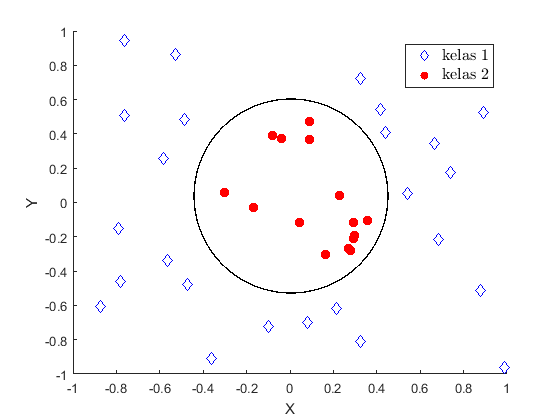
\includegraphics[width=\linewidth]{pics/svm_2db}
    \caption{Ilustrasi Data dalam Dimensi 2}
    \label{fig:svm2d}
  \end{figure}

  \begin{figure}
    \centering
    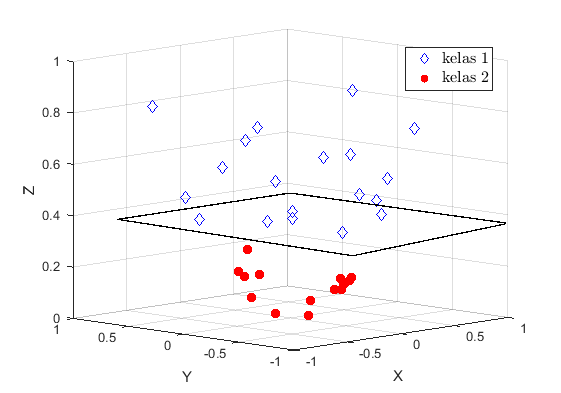
\includegraphics[width=\linewidth]{pics/svm_3db}
    \caption{Ilustrasi Data dalam Dimensi 3}
    \label{fig:svm3d}
  \end{figure}

  Secara matematis, cara kerja SVM dalam melakukan klasifikasi adalah sebagai berikut. Diberikan $l$ sampel \f{training}, $\{\vec x_i,y_i\}$ untuk $i=1,2,\dots,l$; $\vec x_i\in\mathbb{R}^d$; dan $y_i\in\{-1,1\}$. Semua \f{hyperplane} di $\mathbb{R}^d$ memiliki parameter berupa sebuah vektor $\vec w$ dan sebuah konstanta $b$, yang dinyatakan dalam bentuk persamaan
  \begin{equation}
    \vec w\cdot\vec x+b=0.
  \end{equation}
  Diberikan sebuah \f{hyperplane} $(\vec w,b)$ yang memisahkan data, maka terdapat fungsi
  \begin{equation}
    f(\vec x) = sign(\vec w\cdot\vec x+b)
  \end{equation}
  yang mengklasifikasi data \f{training} dengan benar. Syarat data terklasifikasi dengan benar adalah $\forall_i(f(\vec x_i)y_i \geq 1)$.

  Pemetaan ke dimensi ruang yang lebih tinggi membutuhkan proses komputasi yang lebih banyak, serta dapat membuat proses klasifikasi mengalami \f{overfitting}. Karena itu pemetaan vektor tidak dilakukan dalam SVM secara langsung. Pemetaan terjadi secara tidak langsung di dalam \f{kernel function}. \f{Kernel function} adalah fungsi yang digunakan untuk menghitung nilai perkalian dua buah vektor dalam SVM. \f{Kernel function} $K(\vec{x_a},\vec{x_b})$ menerima \f{input} berupa dua buah vektor dan memberikan \f{output} berupa sebuah nilai skalar. Salah satu contoh \f{kernel function} adalah $K(\vec{x_a},\vec{x_b}) = (\vec{x_a}\cdot\vec{x_b}+1)^2$.



  \subsection{Gaussian Mixture Model (GMM)}
  Menurut \cite{6235282}, \f{Gaussian mixture distribution} atau \f{Gaussian mixture model} (GMM) adalah gabungan dari $L$ komponen \f{Gaussian distribution}. Untuk \f{random variable} satu dimensi, $Y$, \f{probability density function (PDF)} dari $Y$ didefinisikan sebagai
  \begin{equation}
    f_Y(y) = \sum_{i=1}^{L}{\omega_i f_{N(\mu_i,\sigma^2_i)}(y)},
  \end{equation}
  di mana $\omega_i$, $\mu_i$, dan $\sigma^2_i$ secara berurutan menyatakan proporsi, rata-rata, dan varian dari komponen ke-i di \f{Gaussian mixture} \citep{4643623}. PDF adalah fungsi pada suatu distribusi \f{random variable} kontinu yang menyatakan probabilitas suatu nilai berada pada interval distribusi tersebut.

  Untuk mempertahankan karakteristik dari \f{probability distribution}, parameter memiliki batasan yaitu, $0<\omega_i\leq1$~dan~$\sum_{i=1}^{L}{\omega_i=1}$. Menurut buku \f{Applied Statistics and Probability for Engineers} yang ditulis oleh \cite{montgomery2013applied}, cara menghitung distribusi dari komponen \f{Gaussian} ke-i, $f_{N(\mu_i,\sigma^2_i)}$, adalah sebagai berikut.
  \begin{equation}
    f_{N(\mu_i,\sigma^2_i)}(x) = \frac{1}{\sqrt{2\pi\sigma^2_i}} e^{(\frac{-(x-\mu_i)^2}{2\sigma^2_i})}.
  \end{equation}

  \cite{5089549} menjelaskan cara menghitung rata-rata ($\mu$) dan varian ($\sigma^2$) dari \f{random variable} $Y$ adalah sebagai berikut.
  \begin{align}
    \mu_Y      &= \sum_{i=1}^{L}{\omega_i\mu_i}\\
    \sigma^2_Y &= \sum_{i=1}^{L}{\omega_i(\sigma^2_i+(\mu_i-\mu_Y)^2)}.
  \end{align}

  Gambar \ref{fig:gmm} menunjukkan \f{probability density} dari \f{random variable} $Y$ yang dimodelkan menggunakan \f{Gaussian distribution} dengan 7 komponen. Jumlah setiap komponen berbobot \f{Gaussian} menghasilkan \f{Gaussian mixture distribution}

  \begin{figure}
    \centering
    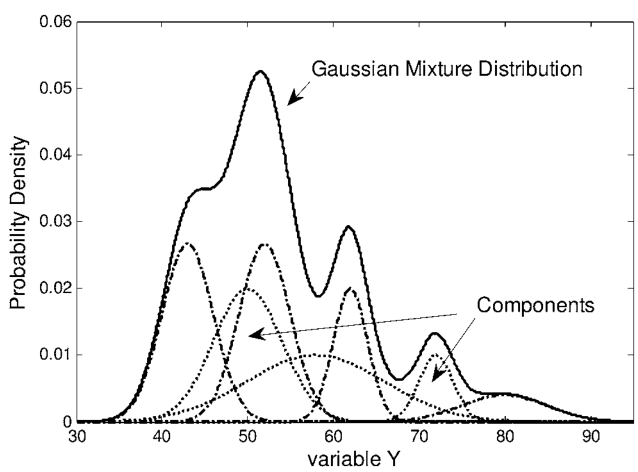
\includegraphics[width=\linewidth]{pics/gmm}
    \caption{\f{Gaussian Mixture Distribution} dengan 7 Komponen}{Sumber gambar: \cite{6235282}}
    \label{fig:gmm}
  \end{figure}

  Keuntungan menggunakan GMM adalah GMM dapat mendekati sembarang PDF selama banyak komponennya terbatas. Biasanya semakin banyak komponen yang ada pada GMM, maka pendekatan tersebut semakin akurat. Metode paling efektif untuk menentukan GMM yang paling mendekati distribusi sampel \f{random variable} $Y$ adalah menggunakan algoritma \f{expectation maximization} \citep{singh2010statistical}.


\section{Evaluasi} \label{chap:evaluasi}
Pada klasifikasi biner, hasil klasifikasi dapat dikategorikan menjadi dua, yaitu \f{true} (+) dan \f{false} (-). Perbandingan hasil klasifikasi dengan hasil yang diharapkan dapat dilihat pada tabel \ref{table:kontingensi}.

\begin{table}
  \centering
  \caption{Kontingensi}
  \begin{tabular}{|c|c|c|}
    \hline
    \multirow{2}{7em}{\textbf{Hasil Klasifikasi}} & \multicolumn{2}{c|}{\textbf{Hasil yang Diharapkan}} \\
    \cline{2-3}
    & + & - \\
    \hline
    + & True Positive (TP) & False Positive (FP) \\
    \hline
    - & False Negative (FN) & True Negative (TN) \\
    \hline
  \end{tabular}
  \label{table:kontingensi}
\end{table}

Dari tabel \ref{table:kontingensi} dapat dihitung beberapa metrik evaluasi, yang dapat digunakan untuk melihat dan menganalisis hasil eksperimen. Beberapa contoh metrik evaluasi antara lain sebagai berikut.

\begin{align}
  Accuracy &= \frac{TP+FN}{TP+FN+FP+TN} \label{equ:accuracy} \\
  Precision &= \frac{TP}{TP+FP} \label{equ:precision} \\
  Recall &= \frac{TP}{TP+FN} \label{equ:recall} \\
  F-measure &= \frac{2 \cdot Precision \cdot Recall}{Precision + Recall} \label{equ:fmeasure}
\end{align}

Nilai-nilai pada metrik evaluasi memiliki makna yang berbeda-beda. \f{Accuracy} (persamaan \ref{equ:accuracy}) menyatakan rasio antara banyaknya hasil klasifikasi yang sesuai dengan hasil yang diharapkan dengan seluruh data yang ada. Dari hasil klasifikasi yang positif (+), rasio antara banyaknya hasil positif yang sesuai dengan yang diharapkan dengan banyaknya hasil klasifikasi yang positif disebut \f{precision} (persamaan \ref{equ:precision}). Kemudian \f{recall} (persamaan \ref{equ:recall}) menyatakan rasio antara banyaknya data yang diklasifikasi positif dengan banyaknya data yang diharapkan positif. Namun terkadang nilai \f{precision} bersaing dengan nilai \f{recall}. Semakin tinggi nilai \f{precision} biasanya membuat nilai \f{recall} semakin rendah, begitu juga sebaliknya, semakin tinggi nilai \f{recall} biasanya membuat nilai \f{precision} semakin rendah. Oleh karena itu dibuatlah nilai \f{F-measure} (persamaan \ref{equ:fmeasure}) yang menyatakan perbandingan nilai \f{precision} dengan \f{recall}.



%-----------------------------------------------------------------------------%
\section{Penelitian Terkait}
%-----------------------------------------------------------------------------%
Penelitian ini membahas sistem \f{automatic speech recognition} (ASR) dalam domain bacaan Al-Qur'an. Beberapa pekerjaan yang sudah dilakukan oleh peneliti sebelumnya terkait bidang ASR dengan domain \quran~antara lain, yang \f{pertama} adalah penelitian yang dilakukan oleh \cite{Muhammad:2010:VCM:1934908.1935467}. Penelitiannya membahas tentang pencocokan suara bacaan Al-Qur'an. Tujuannya adalah membangun sistem yang dapat memberitahukan kesalahan pada pelafalan bacaan \quran~yang tidak sesuai dengan pelafalan yang seharusnya. Penelitiannya menggunakan MFCC sebagai fitur. Namun tidak dijelaskan secara menyeluruh bagaimana proses pencocokan itu dilakukan dalam penelitiannya. Selain itu, terdapat parameter yang ditentukan sendiri oleh penulisnya tanpa penjelasan, seperti penentuan $threshold\_value = 2,6$ dan $matched \geq 3$. Dalam penelitiannya juga tidak dijelaskan mengenai cakupan data yang digunakan.

Penelitian \f{kedua} dilakukan oleh \cite{putra2012developing} yang dimuat dalam jurnalnya, \f{Developing Speech Recognition System for Quranic Verse Recitation Learning Software}. Jurnal tersebut membahas mengenai pengembangan perangkat lunak untuk membantu pembelajaran dalam membaca Al-Qur'an. Penelitian dalam jurnal tersebut menggunakan MFCC sebagai fitur dan GMM sebagai model. Walaupun jurnalnya membahas sampai pada tahap pembuatan perangkat lunak, namun penjelasan mengenai ekstraksi fitur dan teknik pemodelannya masih kurang.

Penelitian \f{ketiga} dilakukan oleh \cite{mohammed2015quranic}. Penelitiannya bertujuan untuk mencegah pengubahan suara bacaan \quran~yang banyak tersebar di \f{internet} dan media sosial secara otomatis. Pengubahan yang dimaksud adalah penambahan, pengurangan, atau kesalahan dalam melafalkan bacaan ayat-ayat Al-Qur'an. Penelitian tersebut menggunakan teks sebagai fitur. Proses ekstraksi teks dari audio lebih kompleks dibandingkan dengan proses ekstraksi MFCC. Untuk mengekstrak teks dari suara setidaknya diperlukan model akustik dan model bahasa. Proses ini menggunakan \f{Hidden Markov Model} (HMM) sebagai model untuk mencari tahu teks mana yang paling memungkinkan untuk menjadi \f{output}. Kekurangan dalam penelitian tersebut adalah laporan penelitiannya hanya mencantumkan hasil yang diharapkan, dan memberikan kesimpulan bahwa untuk Bahasa Arab, fitur yang tepat digunakan adalah MFCC dengan model HMM, berdasarkan teknologi yang berkembang saat ini.%!TEX root = skripsi.tex
%-----------------------------------------------------------------------------%
\chapter{\babTiga}
%-----------------------------------------------------------------------------%


%-----------------------------------------------------------------------------%
\section{Rancangan Arsitektur Sistem}
%-----------------------------------------------------------------------------%
Sistem ASR yang dikembangkan diharapkan dapat memberikan hasil dalam hitungan detik. Karena jika terlalu lama dalam memberikan hasil, maka hal itu akan menghambat pengguna dalam menghafal Al-Qur'an. Selain itu, sistem diharapkan dapat diimplementasikan ke berbagai \f{platform} seperti Windows, Linux, Android, dan lain-lain. Dengan begitu model komputasi yang dihasilkan dalam penelitian ini dapat diaplikasikan dalam berbagai bidang.

Sistem yang akan dibuat dalam penelitian ini sesuai dengan rancangan arsitektur sistem pada gambar \ref{fig:arsitektur_sistem}.
\begin{figure}
  \centering
  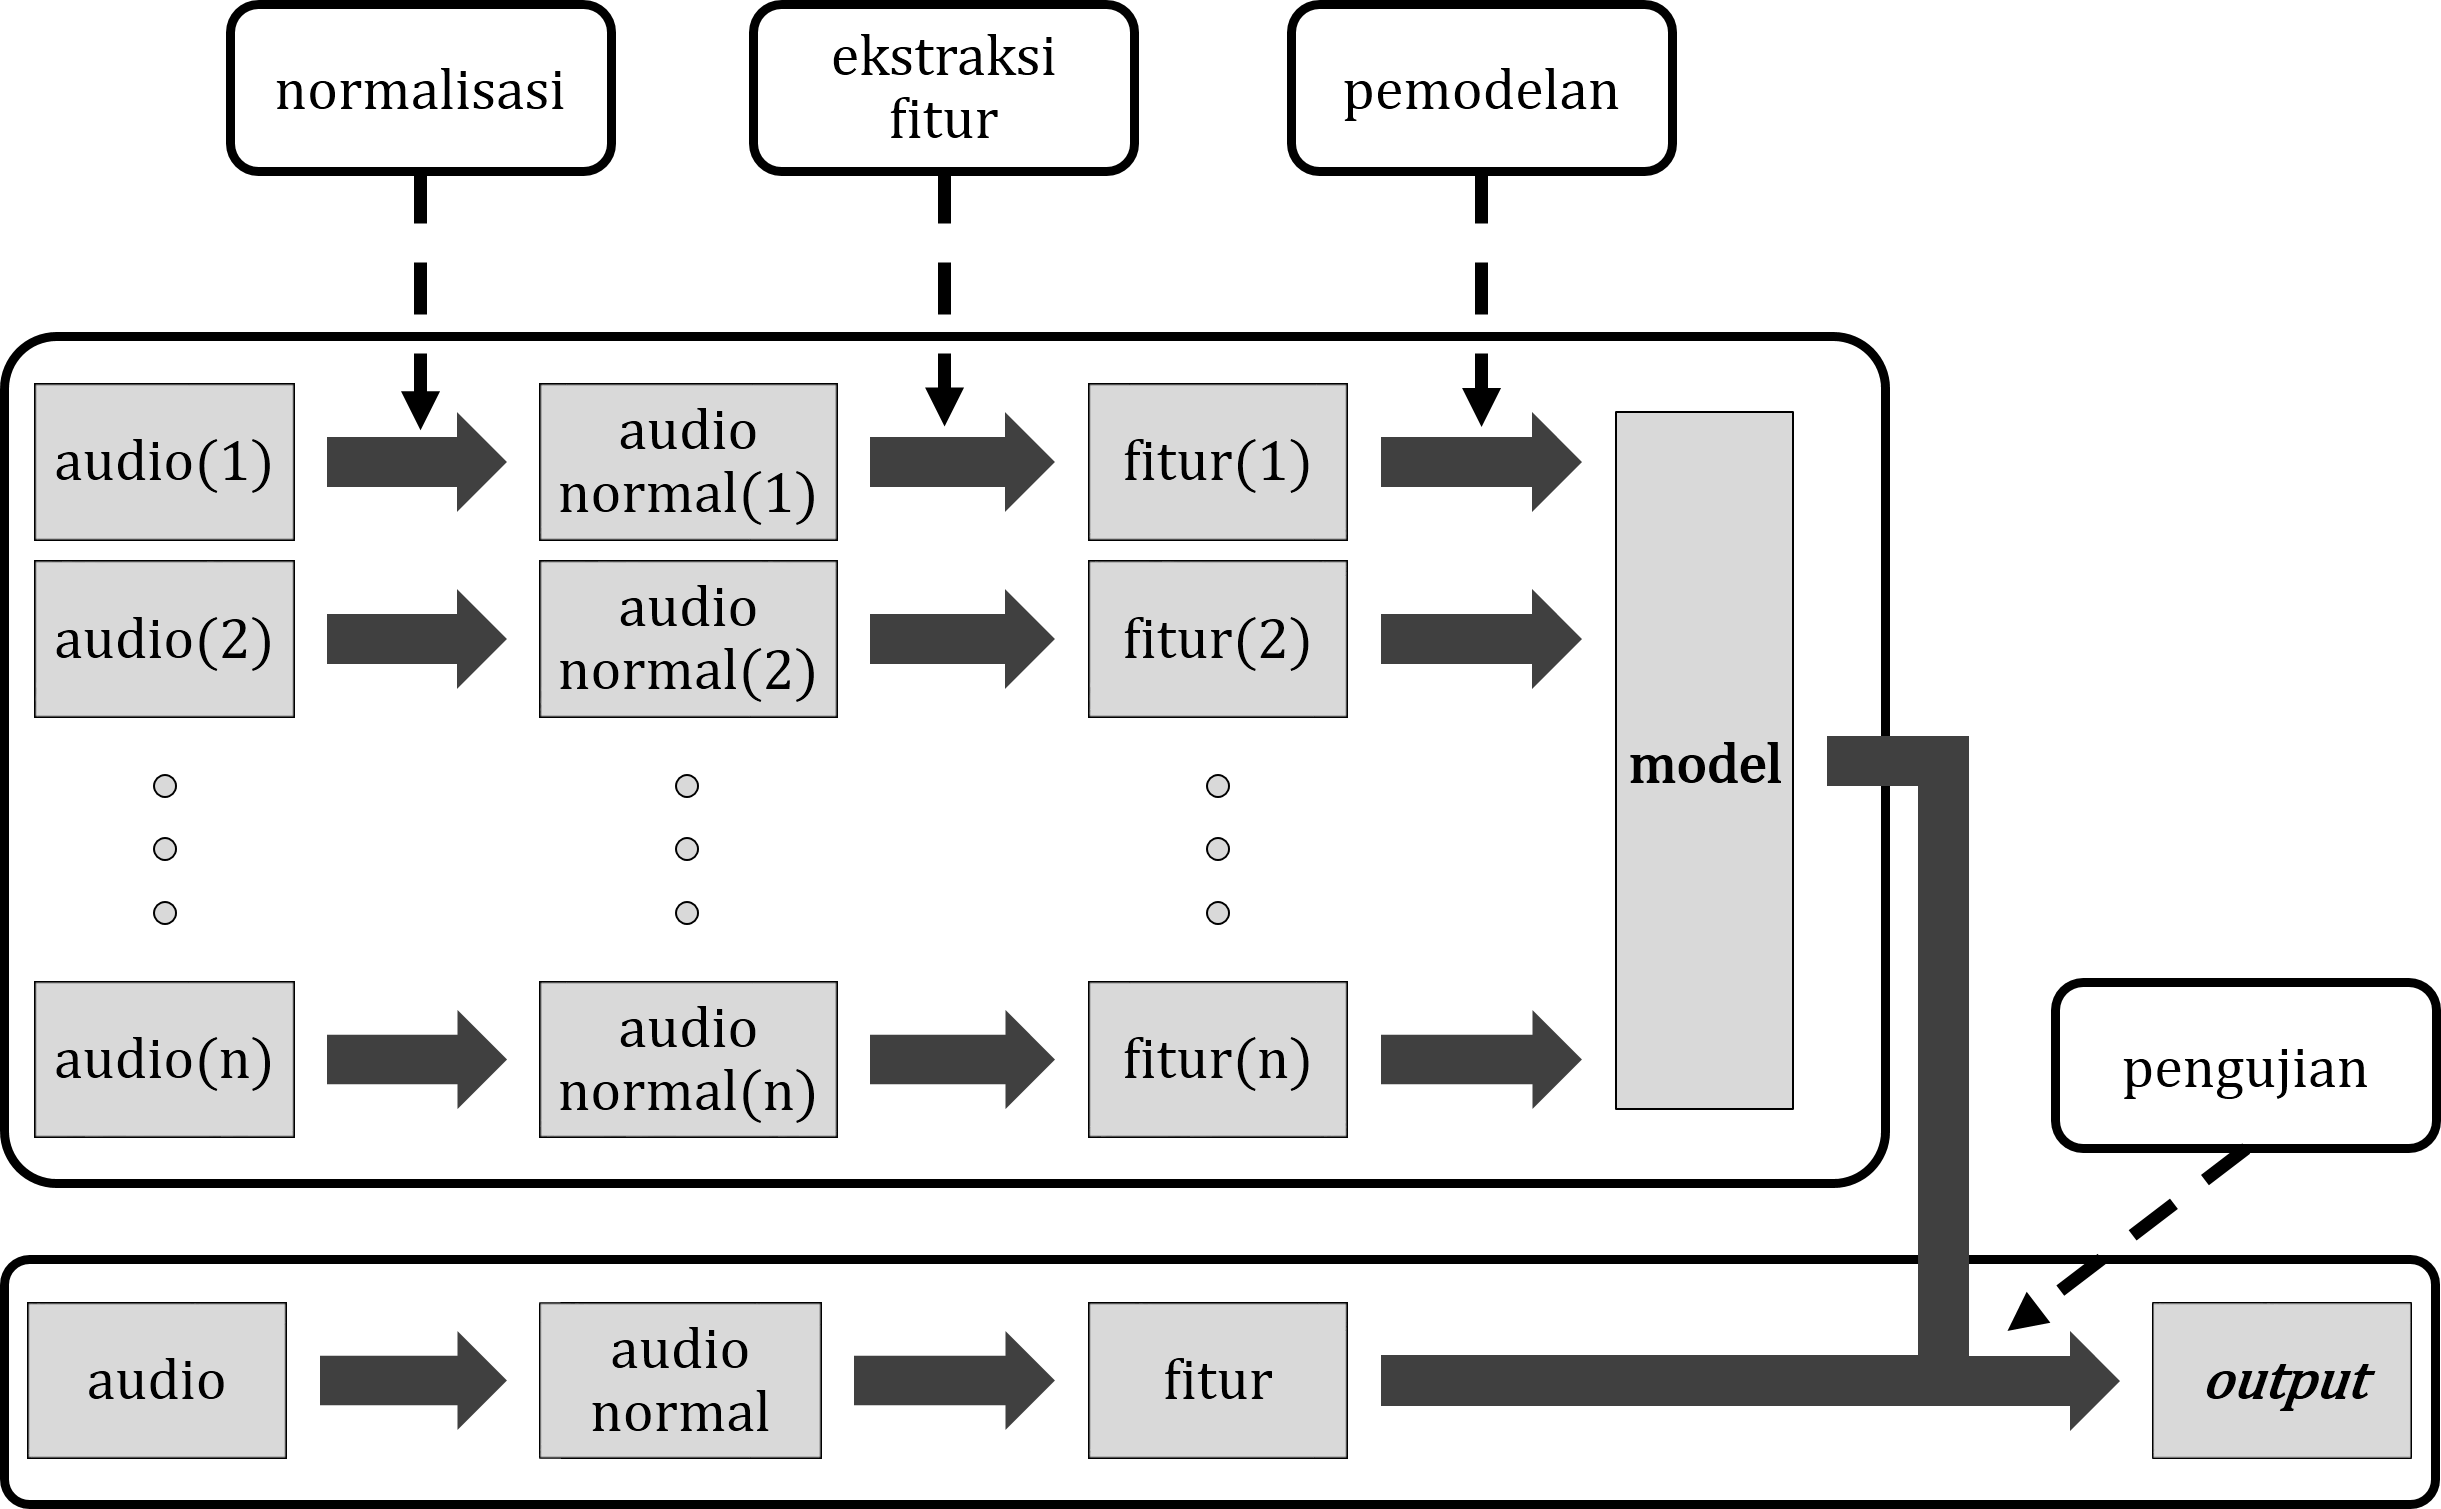
\includegraphics[width=\linewidth]{pics/arsitektur_sistemc}
  \caption{Rancangan Arsitektur Sistem}
  \label{fig:arsitektur_sistem}
\end{figure}

Rancangan arsitektur sistem terbagi menjadi 2 bagian utama, yaitu bagian pemodelan dan bagian pelatihan. Pemodelan adalah proses membuat model dari audio-audio sampel. Pengujian adalah proses memeriksa kebenaran \f{output} yang dihasilkan oleh sistem dengan hasil yang seharusnya. Proses pengujian membutuhkan model dari proses pemodelan.

Alur dari proses pemodelan adalah sebagai berikut.
\begin{enumerate}
  \item Proses normalisasi diterapkan ke setiap audio. Normalisasi yang dilakukan dalam penelitian ini adalah pembuangan \f{silence} atau suara senyap pada audio. Hasil dari proses ini disebut \f{audio normal}.
  \item Proses ekstraksi diterapkan ke setiap audio yang sudah dinormalisasi untuk memperoleh \f{fitur} dari audio tersebut. Penelitian ini menggunakan dua macam fitur, yaitu MFCC dan SDCC. Proses detil ekstraksi fitur akan dijelaskan di Bab \ref{chap:ekstraksi fitur}.
  \item Fitur-fitur hasil proses ekstraksi dijadikan suatu model menggunakan metode klasifikasi, yang akan dijelaskan lebih detil pada Bab \ref{chap:pemodelan}. Satu model digunakan untuk merepresentasikan satu ayat Al-Qur'an.
\end{enumerate}

Alur dari proses pengujian adalah sebagai berikut.
\begin{enumerate}
  \item Proses normalisasi diterapkan ke suatu audio. Normalisasi yang dilakukan pada tahap ini sama dengan normalisasi pada proses pemodelan.
  \item Proses ekstraksi diterapkan ke audio yang sudah dinormalisasi untuk memperoleh \f{fitur} dari audio tersebut. Ekstraksi yang dilakukan pada tahap ini sama dengan ekstraksi pada proses pemodelan.
  \item Fitur hasil proses ekstraksi, ditambah dengan model yang dihasilkan pada proses pemodelan, dimasukkan sebagai \f{input} untuk metode klasifikasi. \f{Output} dari metode klasifikasi berupa label \f{benar} atau \f{salah}. Benar jika audio yang diuji berupa pelafalan bacaan \quran~yang benar menurut sistem dan salah jika selain itu.
\end{enumerate}



%-----------------------------------------------------------------------------%
\section{Data}
%-----------------------------------------------------------------------------%
Penelitian ini memerlukan data berupa berkas audio bacaan seluruh ayat \quran~di juz 30 dari berbagai qari. Karena sistem yang dikembangkan adalah pengenalan suara per ayat, maka data yang diperlukan berupa bacaan \quran~yang sudah dipotong per ayat. Dengan kata lain, satu \f{instance} data merepresentasikan satu ayat \quran~yang dibaca oleh seorang qari. Berikut adalah langkah-langkah untuk memperoleh data tersebut dan memilih data yang tepat untuk digunakan dalam eksperimen.

  \subsection{Pengambilan Data} \label{pengambilan data}
  Data diperoleh dengan cara mengunduh dari beberapa sumber, yaitu \url{http://everyayah.com}, \url{http://tanzil.net}, dan \url{http://recitequran.com}. Tiga sumber tersebut memberi penomoran yang urut pada datanya. Penomoran berkas yang urut memudahkan proses pengunduhan untuk dilakukan secara otomatis menggunakan bantuan program. Nama berkas untuk surat ke-\f{s} dan ayat ke-\f{a} adalah \f{sssaaa.mp3}. Contoh untuk surat ke-78 ayat pertama adalah \f{078001.mp3} dan surat ke-114 ayat ke-6 adalah \f{114006.mp3}. Data yang diambil adalah seluruh surat mulai dari surat ke-78 sampai dengan surat ke-114 (seluruh surat dalam \quran~di juz 30). Total ayat dari surat-surat yang diambil adalah 564 ayat untuk masing-masing qari.

  Di dalam tiga \f{website} yang telah disebutkan sebelumnya tersedia data berupa berkas mp3, di mana satu berkas merepresentasikan satu ayat. Masing-masing berkas memiliki informasi detil yang berbeda-beda, terutama pada \f{duration}, \br, dan \f{channel}. Tabel \ref{table:format berkas 078007 alafasy} menyajikan informasi detil salah satu berkas, yaitu surat An-Naba' ayat 7 dengan qari Mishary Rashid Alafasy.

  \begin{table}
    \centering
    \caption{Informasi Detil Surat An-Naba' Ayat 7 dengan Qari Mishary Rashid Alafasy}
    \begin{tabular}{|c|c|}
      \hline
      Format                         & MPEG Audio \\ \hline
      Format version                 & Version 1 \\ \hline
      Format profile                 & Layer 3 \\ \hline
      Mode                           & Joint stereo \\ \hline
      Mode extension                 & MS Stereo \\ \hline
      Duration                       & 3.866 s \\ \hline
      Bit rate mode                  & Constant \\ \hline
      Bit rate                       & 128 Kbps \\ \hline
      Channel(s)                     & 2 channels \\ \hline
      Sampling rate                  & 44.1 KHz \\ \hline
      Compression mode               & Lossy \\ \hline
      Stream size                    & 60.4 KiB (99\%) \\ \hline
      Writing library                & LAME3.96r \\ \hline
      Encoding settings              & -m j -V 4 -q 3 -lowpass 17.5 -b 128 \\ \hline
    \end{tabular}
    \label{table:format berkas 078007 alafasy}
  \end{table}



  \subsection{Pembuangan Data Duplikat}
  Dari tiga sumber yang telah disebutkan pada Bab \ref{pengambilan data}, diperoleh data bacaan \quran~lebih dari 50 qari berbeda. Namun di antara data-data tersebut, ada beberapa data yang duplikat, yaitu data dengan nama berkas berbeda tetapi sebenarnya memiliki suara yang sama persis. Hal ini dikarenakan ada sedikit perbedaan dari masing-masing sumber data dalam menamai qari. Misalnya dalam \url{http://everyayah.com} terdapat qari dengan nama ``Alafasy\_128kbps'' dan dalam \url{http://tanzil.net} terdapat qari dengan nama ``afasy''. Dua nama tersebut merujuk ke orang yang sama. Untuk mengetahui bahwa dua berkas memiliki konten audio yang sama tidak dilihat dari nama berkasnya, tetapi menggunakan teknik lain. Dalam penelitian ini teknik yang digunakan adalah perbandingan nilai MFCC. Langkah-langkah dari teknik tersebut adalah sebagai berikut.

  \begin{enumerate}
    \item \label{step:pilih ayat} \textbf{Menentukan satu ayat yang akan menjadi acuan}\\
    Ayat yang dipilih boleh yang mana saja, tetapi disarankan bukan ayat pertama dari setiap surat. Ayat pertama dari setiap surat terkadang mengandung bacaan \f{basmalah}\footnote{sebutan untuk bacaan ``\<بِسْمِ اللَّـهِ الرَّحْمَـٰنِ الرَّحِيمِ>''.} yang sebenarnya bukan merupakan bagian dari ayat tersebut, karena bacaan tersebut sifatnya opsional untuk dibaca di awal surat. Ayat yang digunakan pada langkah selanjutnya hanya ayat yang terpilih pada langkah ini. Dalam penelitian ini ayat yang digunakan sebagai acuan adalah ayat ke-6 dari surat ke-114.
    
  	\item \label{step:hitung mfcc} \textbf{Ekstraksi MFCC dari semua qari}\\
  	Dengan mengacu pada ayat yang ditentukan di langkah \ref{step:pilih ayat}, audio bacaan \quran~masing-masing qari diekstrak nilai MFCC-nya. Dalam penelitian ini, parameter koefisien MFCC yang digunakan adalah 13. Hasil dari ekstraksi nilai MFCC berupa matriks berukuran $13\times K$, di mana $K$ merepresentasikan banyaknya \fr. Nilai $K$ bervariasi, bergantung pada durasi audio yang diekstrak. Kemudian, nilai rata-rata dari matriks $13\times K$ pada setiap barisnya dihitung, sehingga terbentuk vektor kolom dengan panjang 13. Vektor kolom adalah matriks yang memiliki tepat 1 kolom. Penghitungan rata-rata dilakukan per baris supaya panjang vektor dari hasil perhitungan ini konstan, yaitu 13. Karena jika yang dihitung nilai rata-rata per \fr, maka hasilnya tentu bervariasi sesuai dengan banyak \fr~dari masing-masing nilai MFCC, yang dipengaruhi oleh durasi audio. Panjang setiap vektor dari langkah ini haruslah sama supaya masing-masing vektor dapat dihitung nilai jaraknya.
  	
  	\item \label{step:hitung jarak} \textbf{Menghitung jarak dari setiap pasang data}\\
    Setiap pasang vektor yang terbentuk dari langkah \ref{step:hitung mfcc} kemudian dihitung nilai jaraknya. Sehingga akan terbentuk matriks D berukuran $N\times N$ yang berisi nilai-nilai jarak tersebut, di mana $N$ adalah banyaknya qari. Baris ke-i dan kolom ke-j menyatakan nilai jarak dari qari ke-i dengan qari ke-j. Penelitian ini menggunakan nilai jarak \f{euclidean distance}\footnote{persamaan \ref{equ:euclideandistance}}.
  	
  	\item \label{step:clustering} \textbf{Mengelompokkan matriks D}\\
    Kumpulan sel di matriks D hasil dari langkah \ref{step:hitung jarak} kemudian dikelompokkan ke dalam 4 kelompok menggunakan teknik \f{k-means clustering}. Pembagian ke dalam 4 kelompok ini dimaksudkan supaya data terbagi ke dalam kelompok \f{mirip}, \f{sedikit mirip}, \f{tidak terlalu mirip}, dan \f{tidak mirip}. Kelompok yang mengandung nilai terendah adalah kelompok \f{mirip} yang ditetapkan sebagai pasangan data yang duplikat. Jika pembagiannya hanya 3 atau 2 kelompok saja, maka akan ada pasangan-pasangan data yang hanya \f{sedikit mirip}, yang jika diamati secara manual berbeda (tidak duplikat), tetapi masuk ke dalam kelompok \f{mirip}, sehingga dianggap duplikat. Dari langkah ini akan dihasilkan matriks C yang berukuran sama dengan matriks D, di mana setiap sel pada matriks C berisi label kelompok. Nilai sel pada baris ke-i dan kolom ke-j menyatakan level kemiripan qari ke-i dengan qari ke-j.
  	
  	\item \textbf{Membuang data mirip}\\
    Dengan mengacu pada matriks C yang diperoleh pada langkah \ref{step:clustering}, setiap pasangan data yang memiliki hubungan \f{mirip}, salah satu dari keduanya dihilangkan dari himpunan data eksperimen pada penelitian ini.
  \end{enumerate}

  \subsection{Penyaringan Data}
  Setelah data yang terkumpul dipastikan tidak mengandung data yang duplikat, maka langkah selanjutnya adalah menyaring data. Proses ini dilakukan secara manual. Adapun kriteria data yang lolos saringan adalah sebagai berikut:
  \begin{enumerate}
    \item \textbf{Terdengar jelas dan bacaannya benar}.\\
    Suara bacaan \quran~harus terdengar jelas oleh pendengaran manusia. Data yang tidak jelas menurut pendengaran manusia tidak sesuai standar dalam penelitian ini, sehingga tidak disertakan dalam eksperimen. Di samping itu, bacaan dalam data tersebut juga harus sesuai dengan cara membaca \quran~yang benar.

    \item \textbf{Tidak mengandung bacaan \f{basmalah}}.\\
    Sebagian qari mengawali pembacaan ayat pertama di setiap surat dengan \f{basmalah}. Karena bacaan ini bukan bagian dari ayat pertama dan sifatnya opsional, ada qari yang membacanya dan ada juga yang tidak. Baik membaca \f{basmalah} maupun tidak, keduanya benar menurut aturan membaca Al-Qur'an. Oleh karena itu, dalam penelitian ini perlu diterapkan standar, yaitu data yang digunakan hanya data yang tidak mengandung bacaan \f{basmalah}.

    \item \textbf{Tidak mengandung pantulan suara}.\\
    Beberapa suara bacaan \quran~mengandung pantulan suara atau \f{echo}. \f{Echo} dalam rekaman bacaan \quran~disebabkan oleh efek audio digital yang sengaja ditambahkan untuk memberikan kesan bagus. Namun hal itu justru akan mengganggu proses klasifikasi. Maka data yang mengandung \f{echo} tidak disertakan dalam eksperimen dalam penelitian ini.
  \end{enumerate}

  Informasi mengenai data yang tersisa setelah proses pembuangan data duplikat dan penyaringan, dapat dilihat pada tabel \ref{table:data yang tersisa}.
  
  \begin{table}
    \centering
    \caption{Data yang Tersisa}
    \begin{tabular}{|c|c|}
      \hline
      Banyak Qari & 40 qari \\ \hline
      Surat Mulai & An-Naba' (surat ke-78) \\ \hline
      Surat Selesai & An-Nas (surat ke-114) \\ \hline
      Banyak Surat & 37 surat \\ \hline
      Banyak Ayat & 564 ayat \\ \hline
      Total Seluruh \f{Instance} & 22,560 \f{instance} \\ \hline
    \end{tabular}
    \label{table:data yang tersisa}
  \end{table}



\section{Perangkat dan Fungsi Pendukung}
  \subsection{Perangkat Pendukung}
  Perangkat pendukung dalam eksperimen ini terdiri dari dua komponen, yaitu \f{hardware} dan \f{software}. Spesifikasi \f{hardware} komputer yang digunakan dapat dilihat pada tabel \ref{table:spesifikasi hardware}.

  \begin{table}
    \centering
    \caption{Spesifikasi \f{Hardware}}
    \begin{tabular}{|c|c|}
      \hline
      Processor & i7-4770S \\ \hline
      Banyak Core & 8 core \\ \hline
      Frekuensi Processor & 3.1 GHz per core \\ \hline
      RAM & 8 GB \\ \hline
    \end{tabular}
    \label{table:spesifikasi hardware}
  \end{table}

   \f{Software} yang digunakan untuk membantu eksperimen ini adalah MATLAB\footnote{http://mathworks.com} versi R2013b. \f{Software} ini dipilih karena menyediakan banyak fungsi yang dapat membantu jalannya eksperimen, seperti fungsi \f{plot} untuk menampilkan grafik dari suatu data, fungsi \f{mean} untuk menghitung rata-rata, dan lain-lain.

  \subsection{Fungsi Pendukung} \label{fungsipendukung}
  MATLAB menyediakan banyak fungsi yang dapat digunakan untuk membantu eksperimen. Namun selain fungsi-fungsi yang sudah disediakan MATLAB, diperlukan fungsi tambahan untuk menjalankan eksperimen ini, antara lain sebagai berikut.
  \begin{enumerate}
    \item audioread\\
    \f{audioread} adalah fungsi untuk membaca berkas mp3 yang sudah tersedia di MATLAB mulai dari versi R2012b\footnote{http://www.mathworks.com/help/matlab/ref/audioread.html}. Jika fungsi \f{audioread} belum ada di MATLAB, maka fungsi alternatifnya adalah fungsi \f{wavread}. Fungsi \f{audioread} menerima \ioa~berupa \f{string} yang menyatakan lokasi penyimpanan berkas, lalu memberikan \iob~berupa matriks sinyal $N \times C$ dan \br. $N$ menyatakan panjang sinyal, sedangkan $C$ menyatakan banyaknya \f{channel}.

    \item mfcc\\
    \f{mfcc} adalah fungsi untuk menghitung MFCC. Implementasi fungsi \f{mfcc} menggunakan \f{source code} dari \href{http://www.mathworks.com/matlabcentral/fileexchange/32849-htk-mfcc-matlab}{HTK MFCC MATLAB}\footnote{http://www.mathworks.com/matlabcentral/fileexchange/32849-htk-mfcc-matlab}. Fungsi \f{mfcc} membutuhkan parameter seperti yang tercantum dalam tabel \ref{table:parametermfcc}.

    \begin{table}
      \centering
      \caption{Parameter Fungsi \f{mfcc}}
      \begin{tabular}{|l|l|}
        % mfcc( speech, fs, Tw, Ts, alpha, window, R, M, N, L )
        \hline
        \textbf{Nama Parameter} & \textbf{Keterangan} \\ \hline
        Speech & Data audio dalam bentuk matriks $nx1$ \\ \hline
        Fs & \f{Bit rate} \\ \hline
        Tw & \f{Analysis frame duration} (ms) \\ \hline
        Ts & \f{Analysis frame shift} (ms) \\ \hline
        Alpha & \f{Preemphasis coefficient} \\ \hline
        Window & \f{Windowing function} \\ \hline
        R & \f{Frequency range} \\ \hline
        M & Banyaknya \f{filterbank channels} \\ \hline
        C & Banyaknya \f{cepstral coefficients} \\ \hline
        L & Parameter \f{cepstral sine lifter} \\ \hline
      \end{tabular}
      \label{table:parametermfcc}
    \end{table}

    \item mfcc2sdc\\
    \f{mfcc2sdc} adalah fungsi untuk menghitung SDCC. Implementasi fungsi tersebut diperoleh dari \f{source code} di \href{http://www.mathworks.com/matlabcentral/fileexchange/31478-shifted-delta-coefficients--sdc--computation-from-mel-frequency-cepstral-coefficients--mfcc-}{HTK MFCC MATLAB}\footnote{http://www.mathworks.com/matlabcentral/fileexchange/31478-shifted-delta-coefficients--sdc--computation-from-mel-frequency-cepstral-coefficients--mfcc-}. Fungsi \f{mfcc2sdc} membutuhkan parameter seperti yang tercantum pada tabel \ref{table:parametersdcc}.

    \begin{table}
      \centering
      \caption{Parameter Fungsi \f{mfcc2sdc}}
      \begin{tabular}{|l|l|}
        % mfcc2sdc(CepCoeff,d,P,K)
        \hline
        \textbf{Nama Parameter} & \textbf{Keterangan} \\ \hline
        CepCoeff & Matriks MFCC dalam bentuk KxC, di mana K menyatakan \\
        &~ banyaknya \fr~dan C menyatakan banyaknya koefisien MFCC \\ \hline
        D & Nilai \f{shift} untuk \f{delta computation} \\ \hline
        P & Nilai \f{shift} untuk \fr~selanjutnya \\ \hline
        K & Banyaknya blok di mana koefisien \f{delta} disambungkan \\ \hline
      \end{tabular}
      \label{table:parametersdcc}
    \end{table}

    % \item kmeans\\
    % \item svmtrain\\
    % \item gmdistribution.fit\\

  \end{enumerate}%!TEX root = skripsi.tex
%-----------------------------------------------------------------------------%
\chapter{\babEmpat} \label{eksperimen}
%-----------------------------------------------------------------------------%

\section{Normalisasi Data}
Data yang sudah diperoleh perlu dinormalisasi terlebih dahulu untuk membuang \f{noise} yang dapat mengganggu jalannya eksperimen. Normalisasi dilakukan dengan cara membuang suara senyap atau \f{silence}. Ada beberapa teknik yang digunakan untuk membuang \f{silence}. Salah satu teknik klasik dan populer yang digunakan untuk membuang \f{silence} pada suara adalah kombinasi \f{short term energy} (STE) dengan \f{zero crossing rate} (ZCR) \citep{rabiner1978digital}. \cite{saha2005new} memaparkan pendekatan lain yang lebih baik akurasinya dalam membuang \f{silence} jika dibandingkan dengan STE maupun kombinasi ZCR dengan STE, yaitu dengan memodelkan sinyal audio menggunakan distribusi \f{Gaussian}.

Penelitian ini menggunakan pendekatan yang dipaparkan oleh \cite{saha2005new} dalam membuang \f{silence}, dengan langkah-langkah sebagai berikut.

\begin{enumerate}
	\item \label{satu} Hitung rata-rata ($\mu$) dan standar deviasi ($\sigma$) dari 10 ms sampel pertama pada audio. Jika $fs$ menyatakan \br~dari audio, maka terdapat sebanyak $s$ sampel dalam 10 ms.
	\begin{align}
    s &= 0.01\cdot fs \\
		\mu &= \frac{\sum_{i=1}^{s}x(i)}{s} \\
		\sigma &= \sqrt{\frac{\sum_{i=1}^{s}(x(i)-\mu)^2}{s}}
	\end{align}
	\f{Background noise} juga dikenali dari berdasarkan nilai rata-rata ($\mu$) dan standar deviasinya ($\sigma$).

	\item Periksa apakah jarak \f{Mahalanobis} mulai dari sampel pertama sampai dengan sampel terakhir pada audio lebih dari $3$ atau tidak. Jarak \f{Mahalanobis} dihitung menggunakan fungsi $f$ sebagai berikut.
	\begin{equation}
		d(x) = \frac{|x-\mu|}{\sigma}
	\end{equation}
	Nilai $3$ dipilih karena pada distribusi \f{Gaussian}, 99.7\% data memiliki nilai jarak \f{Mahalanobis} $\leq3$. Gambar \ref{fig:distribusinormal} menunjukkan persebaran data pada distribusi \f{Gaussian}.

	\begin{figure}
		\centering
		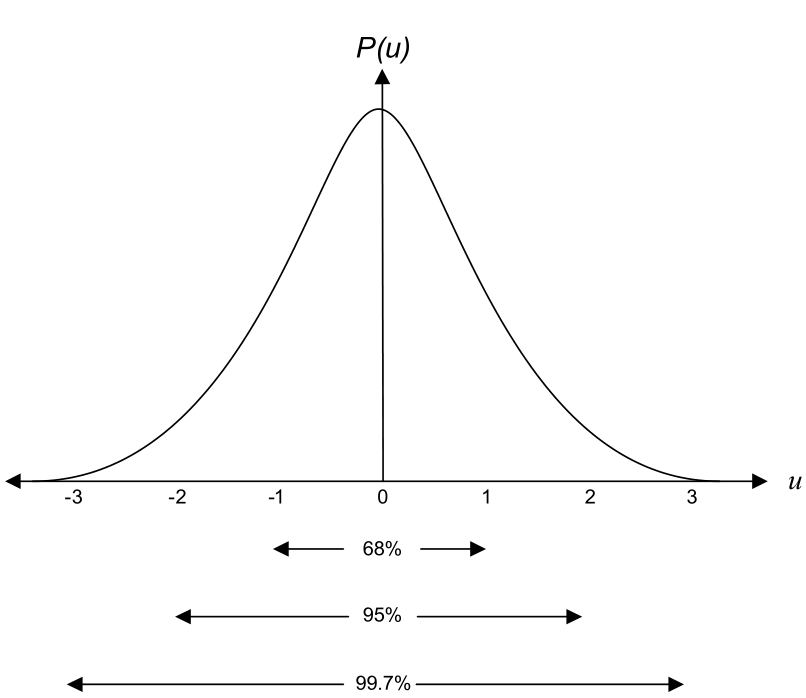
\includegraphics[width=0.85\linewidth]{pics/distribusi_normal}
		\caption{Distribusi \f{Gaussian} Terhadap Nilai Jarak \f{Mahalanobis}}{Sumber gambar: \cite{saha2005new}}
		\label{fig:distribusinormal}
	\end{figure}

	\item Tandai sampel yang dianggap bukan sebagai \f{silence} (selanjutnya disebut \f{voiced}) dengan 1 dan sampel yang dianggap sebagai \f{silence} dengan 0. Bagi keseluruhan sinyal audio ke dalam beberapa bagian yang tidak saling \f{overlap}, dengan durasi pada setiap bagian adalah 10 ms.

	\item \label{empat} Asumsikan ada $M$ sampel yang bernilai 0 dan $N$ sampel yang bernilai 1. Jika $M \geq N$, maka ubah setiap tanda 1 menjadi tanda 0, dan sebaliknya.

	\item Kumpulkan seluruh bagian yang dianggap sebagai \f{voiced}, yaitu bagian-bagian yang bertanda 1 hasil dari langkah \ref{satu} sampai langkah \ref{empat}.
\end{enumerate}


	
\section{Ekstraksi Fitur} \label{chap:ekstraksi fitur}
Ekstraksi fitur adalah proses mengubah data \f{input} menjadi himpunan fitur-fitur yang dapat merepresentasikan data \f{input} dengan baik. Ekstraksi fitur merupakan bentuk istimewa dari \f{dimensionality reduction} \citep{Soft-Computational}. \cite{wyse1980critical} menjelaskan bahwa ekstraksi fitur adalah proses yang mengekstrak himpunan fitur-fitur baru dari fitur asli melalui serangkaian fungsi pemetaan. Penelitian ini menggunakan dua jenis fitur, yaitu \f{mel frequency cepstral coefficient} (MFCC) dan \f{shifted delta cepstral coefficient} (SDCC).

% Data jenis mp3 terlalu kompleks untuk diklasifikasi secara langsung menggunakan metode-metode yang ada saat ini. Selain itu, banyak informasi tidak perlu atau \f{noise} yang terdapat pada sebuah berkas mp3. Untuk itu diperlukan proses ekstraksi fitur. Dengan proses ini diharapkan hanya informasi penting saja yang terambil dari sebuah berkas mp3 dan memiliki bentuk yang tidak terlalu kompleks.

\subsection{Ekstraksi Fitur MFCC} \label{chap:ekstrak fitur mfcc}
Ekstraksi fitur MFCC menggunakan fungsi \f{mfcc} yang telah dijelaskan di Bab \ref{fungsipendukung}. Fungsi \f{mfcc} pada eksperimen ini dipanggil dengan parameter fungsi yang dijelaskan pada tabel \ref{table:pemanggilanmfcc}.
\begin{table}
	\centering
  \caption{Parameter Pemanggilan Fungsi \f{mfcc}}
  \begin{tabular}{|l|l|}
    % mfcc( speech, fs, Tw, Ts, alpha, window, R, M, N, L )
    \hline
    \textbf{Nama Parameter} & \textbf{Nilai Parameter} \\ \hline
    Tw & 25 ms \\ \hline
    Ts & 10 ms \\ \hline
    Alpha & 0.97 \\ \hline
    Window & \f{hamming window}  \\ \hline
    R & [300 3700] \\ \hline
    M & 20 \\ \hline
    C & 13 \\ \hline
    L & 22 \\ \hline
  \end{tabular}
  \label{table:pemanggilanmfcc}
 \end{table}

Berikut adalah langkah-langkah untuk memproses fitur MFCC.
\begin{enumerate}
  \item Tentukan nilai \br~untuk dimasukkan dalam perhitungan MFCC, yang akan mempengaruhi durasi audio. Durasi sebuah audio (dalam detik), $d$, dapat dihitung dengan rumus
  \begin{equation}
    d = \frac{L}{fs}, 
  \end{equation}
  di mana $L$ adalah panjang \fr~audio dan $fs$ adalah \br. Banyaknya \fr~(panjang kolom) pada hasil ekstraksi nilai MFCC dipengaruhi oleh durasi audionya. Maka untuk menyamakan panjang kolom hasil ekstraksi MFCC, durasi audio-audio yang akan diproses harus disamakan terlebih dahulu. Durasi yang digunakan untuk mengekstrak nilai MFCC pada satu ayat tertentu adalah \f{nilai rata-rata durasi} keseluruhan audio dari berbagai qari pada ayat tersebut. Setelah diperoleh nilai rata-rata durasi, $\bar{d}$, langkah selanjutnya adalah membuat masing-masing audio memiliki durasi yang sama, dengan cara mengubah nilai $fs$ masing-masing audio. Jika diberikan nilai $\bar{d}$ dan $L$, maka nilai $fs$ yang baru, $\widehat{fs}$, dihitung menggunakan rumus
  \begin{equation}
    \widehat{fs} = \frac{L}{\bar{d}}.
  \end{equation}


	\item Panggil fungsi \f{mfcc} dengan parameter yang telah disebutkan pada tabel \ref{table:pemanggilanmfcc} dan nilai \br~sama dengan $\widehat{fs}$, sehingga memberikan \f{output} berupa matriks MFCC 13x$K$, di mana $K$ menyatakan banyaknya \fr.

	\item Buang matriks MFCC pada baris pertama, karena nilai tersebut merupakan log energi yang bukan merupakan bagian dari fitur dalam eksperimen ini. Sehingga matriks MFCC yang tersisa berukuran $12\times K$.

	\item Hitung nilai rata-rata pada setiap \fr~matriks MFCC. Perhitungan tersebut akan menghasilkan vektor kolom, $\vec v$, dengan panjang $K$. Vektor kolom adalah matriks yang hanya memiliki satu baris.

	\item Selanjutnya vektor tersebut dipendekkan dengan cara sebagai berikut.
	\begin{enumerate}[label*=\arabic*.]
		\item Tentukan nilai $s$ (\f{shift}). $s = \left\lceil\frac{K}{30}\right\rceil$.
		\item Tentukan nilai $w$ (\f{width}). $w = \left\lceil1.5 \times s\right\rceil$.
		\item Setiap $s$ elemen sekali, hitung nilai rata-rata dari $w$ elemen berurutan pada vektor $\vec{v}$.
	\end{enumerate}
	Hasil pemendekan tersebut berupa vektor $\widehat{\vec{v}}$ dengan panjang $\widehat K$, di mana \[ \widehat{K} = \left\lceil \frac{K-w+1}{s} \right\rceil = \left\lceil \frac{K-1.5\left\lceil\frac{K}{30}\right\rceil+1}{\left\lceil\frac{K}{30}\right\rceil} \right\rceil \leq 29. \] Tujuan dari pemendekan vektor ini adalah untuk mengurangi kompleksitas fitur sehingga diharapkan hasil klasifikasi akan lebih akurat.
  
  Gambar \ref{fig:alurekstraksifiturmfcc} menunjukkan alur proses ekstraksi fitur MFCC.
  \begin{figure}
    \centering
    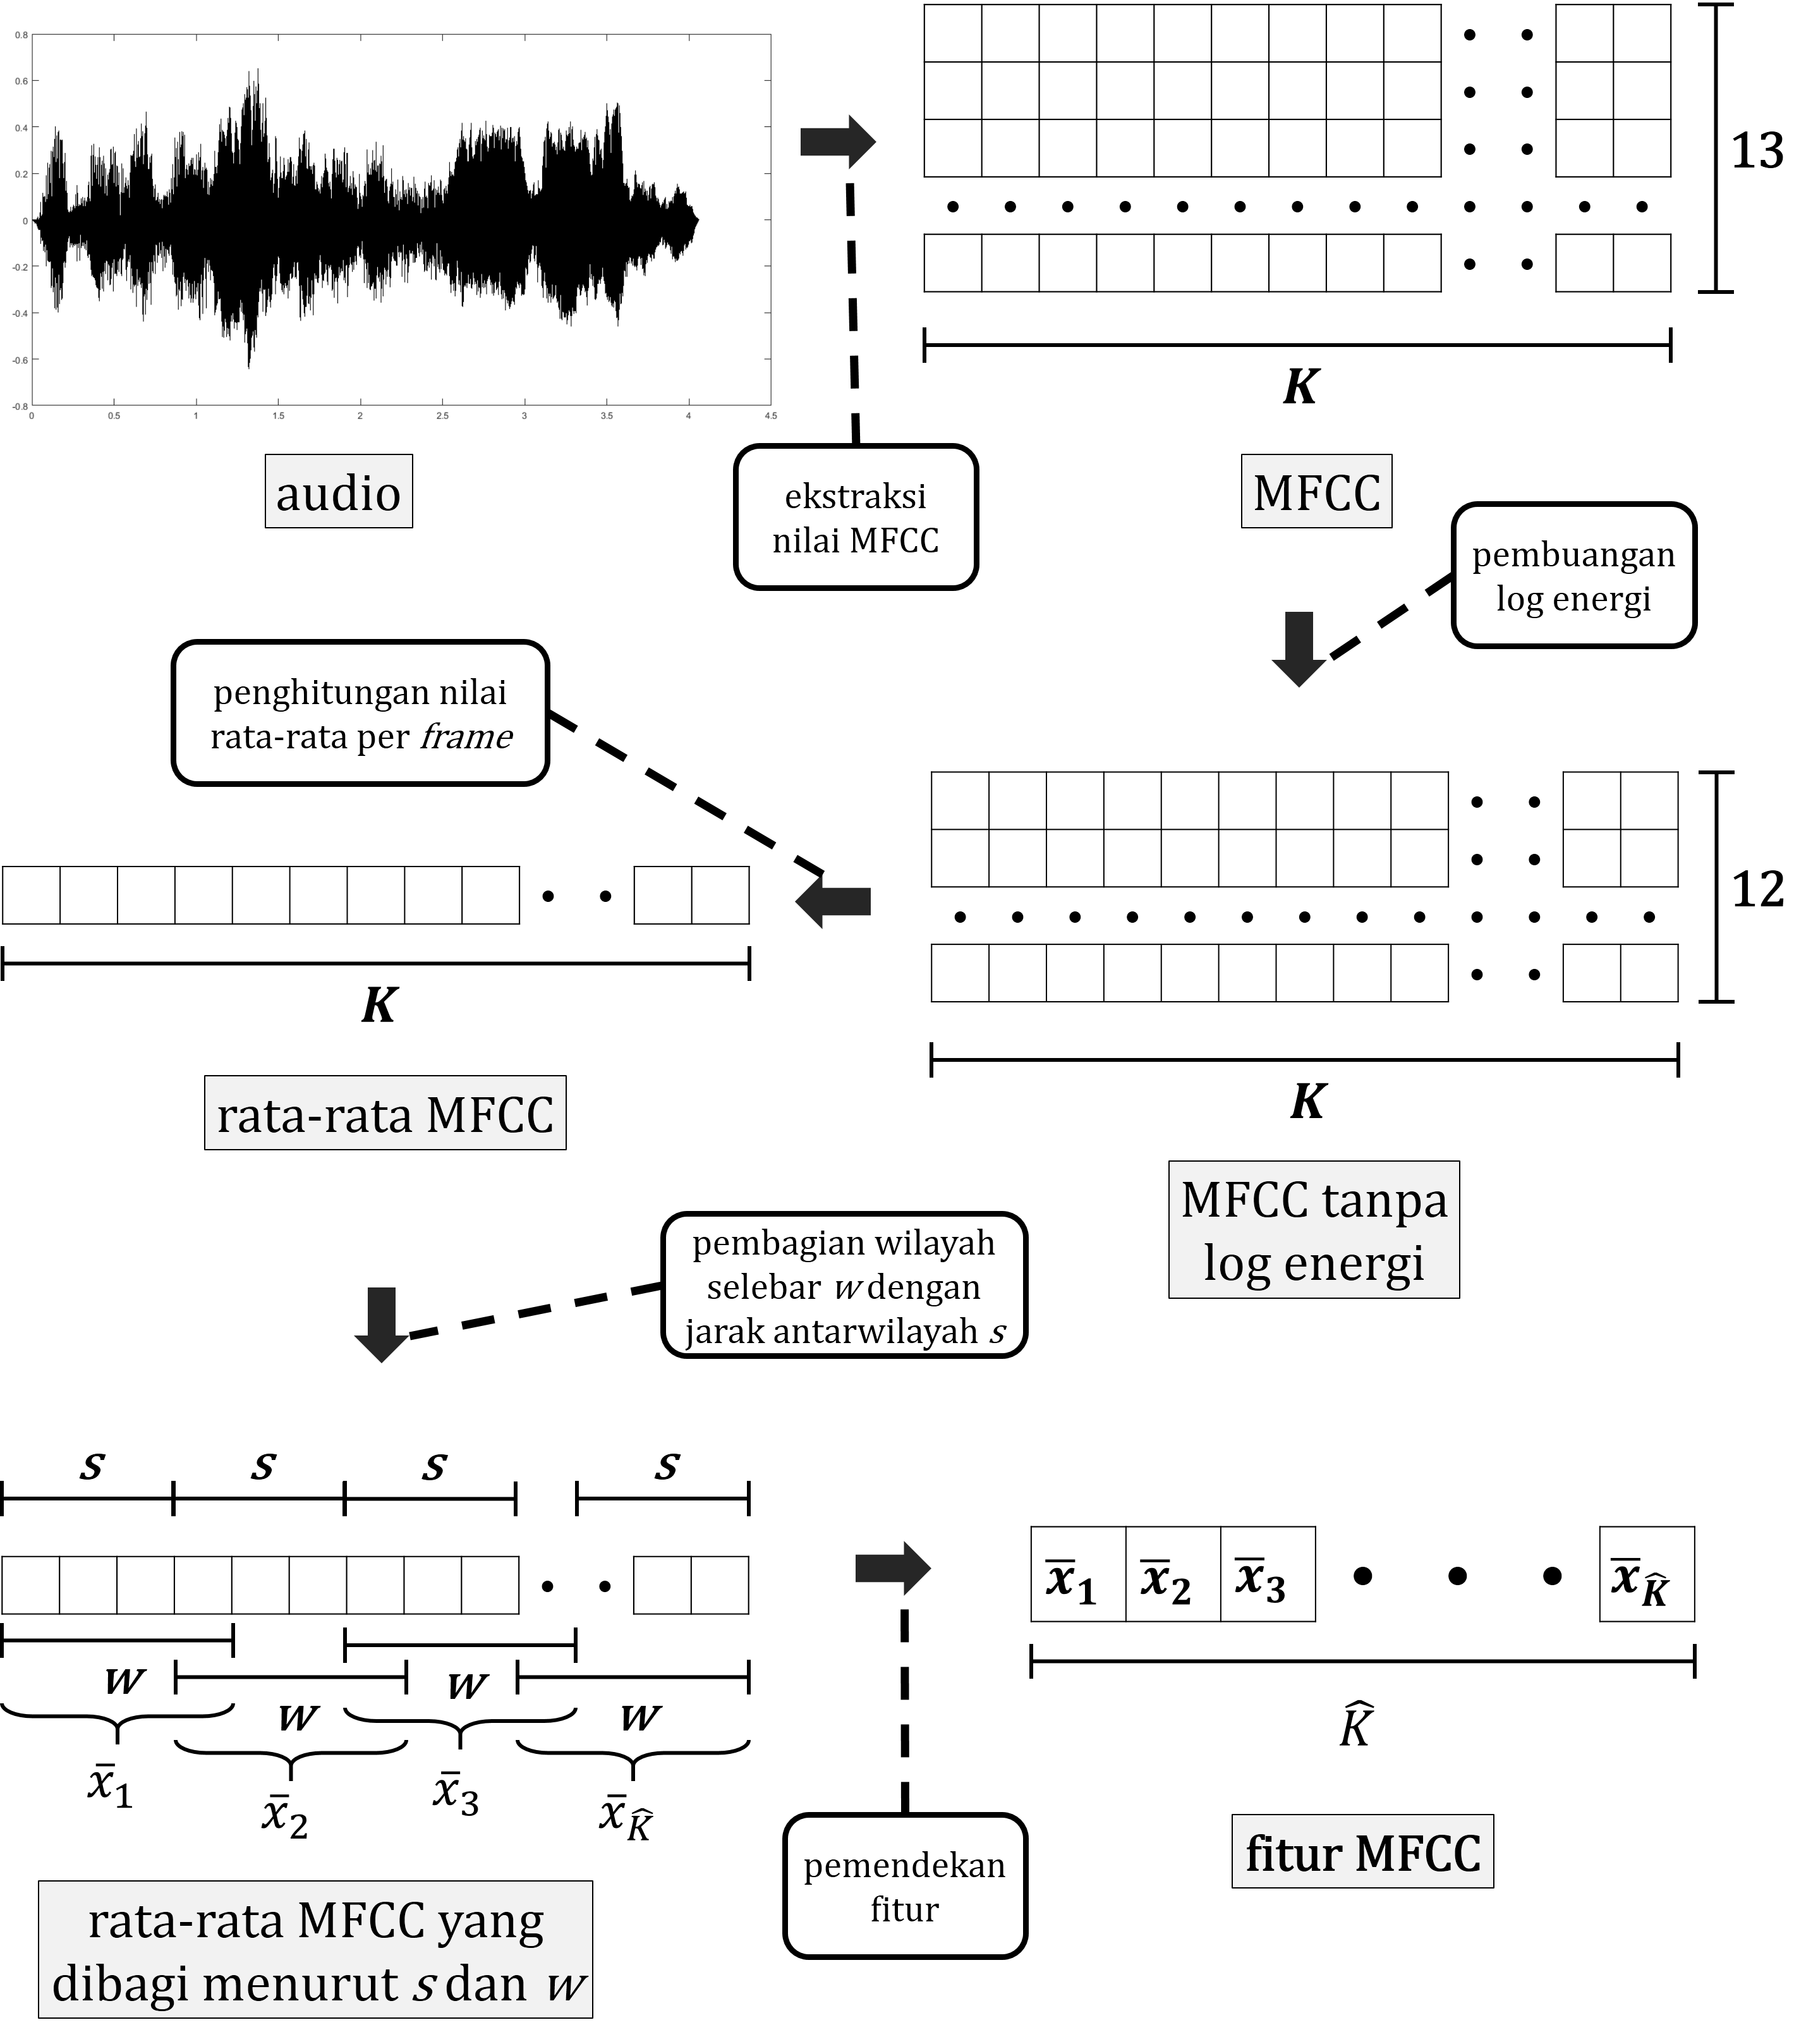
\includegraphics[width=\linewidth]{pics/ekstraksi_mfcc_v3}
    \caption{Alur Ekstraksi Fitur MFCC}
    \label{fig:alurekstraksifiturmfcc}
  \end{figure}
\end{enumerate}



\subsection{Ekstraksi Fitur SDCC}
Ekstraksi fitur SDCC menggunakan fungsi \f{mfcc2sdc} yang telah dijelaskan di Bab \ref{fungsipendukung}. Fungsi \f{mfcc2sdc} pada eksperimen ini dipanggil dengan parameter fungsi yang dijelaskan pada tabel \ref{table:pemanggilansdcc}.
\begin{table}
	\centering
  \caption{Parameter Pemanggilan Fungsi \f{mfcc2sdc}}
  \begin{tabular}{|l|l|}
    % mfcc2sdc(CepCoeff,d,P,K)
    \hline
    \textbf{Nama Parameter} & \textbf{Nilai Parameter} \\ \hline
    D (nilai \f{shift} untuk \f{delta computation}) & 1 \\ \hline
    P (nilai \f{shift} untuk \fr~selanjutnya) & 3 \\ \hline
    K (banyaknya blok di mana koefisien \f{delta} disambungkan) & 3 \\ \hline
  \end{tabular}
  \label{table:pemanggilansdcc}
 \end{table}

Berikut adalah langkah-langkah untuk memproses fitur SDCC.
\begin{enumerate}
  \item Hitung nilai MFCC menggunakan fungsi \f{mfcc} seperti sudah dijelaskan di Bab \ref{chap:ekstrak fitur mfcc}, langkah 1 sampai 3, sehingga diperoleh nilai MFCC berupa matriks berukuran $12\times K$. Nilai MFCC berukuran $12\times K$ perlu di-\f{transpose} terlebih dahulu menjadi ukuran $K\times12$ untuk menyesuaikan kebutuhan fungsi \f{mfcc2sdc}, yaitu baris sebagai \fr~dan kolom sebagai koefisien.

	\item Panggil fungsi \f{mfcc2sdc} dengan parameter yang telah disebutkan pada tabel \ref{table:pemanggilansdcc}, sehingga memberikan \f{output} berupa matriks SDCC $36\times L$, di mana $L$ menyatakan banyaknya \fr.

	\item Hitung nilai rata-rata pada setiap \fr~matriks SDCC. Perhitungan tersebut akan menghasilkan vektor kolom, $w$, dengan panjang $L$.

	\item Selanjutnya vektor tersebut dipendekkan dengan cara sebagai berikut.
	\begin{enumerate}[label*=\arabic*.]
		\item Tentukan nilai $s$ (\f{shift}). $s = \left\lceil\frac{L}{30}\right\rceil$.
		\item Tentukan nilai $w$ (\f{width}). $w = \left\lceil1.5\times s\right\rceil$.
		\item Setiap $s$ elemen sekali, hitung nilai rata-rata dari $w$ elemen berurutan pada vektor $\vec{w}$.
	\end{enumerate}
	Hasil pemendekan tersebut berupa vektor $\widehat{\vec{w}}$ dengan panjang $\widehat L$, di mana \[ \widehat L = \left\lceil \frac{L-w+1}{s} \right\rceil = \left\lceil \frac{L-1.5\left\lceil\frac{L}{30}\right\rceil+1}{\left\lceil\frac{L}{30}\right\rceil} \right\rceil \leq 29. \] Tujuan dari pemendekan vektor ini adalah untuk mengurangi kompleksitas fitur sehingga diharapkan hasil klasifikasi akan lebih akurat.

  Gambar \ref{fig:alurekstraksifitursdcc} menunjukkan alur proses ekstraksi fitur SDCC.
  \begin{figure}
    \centering
    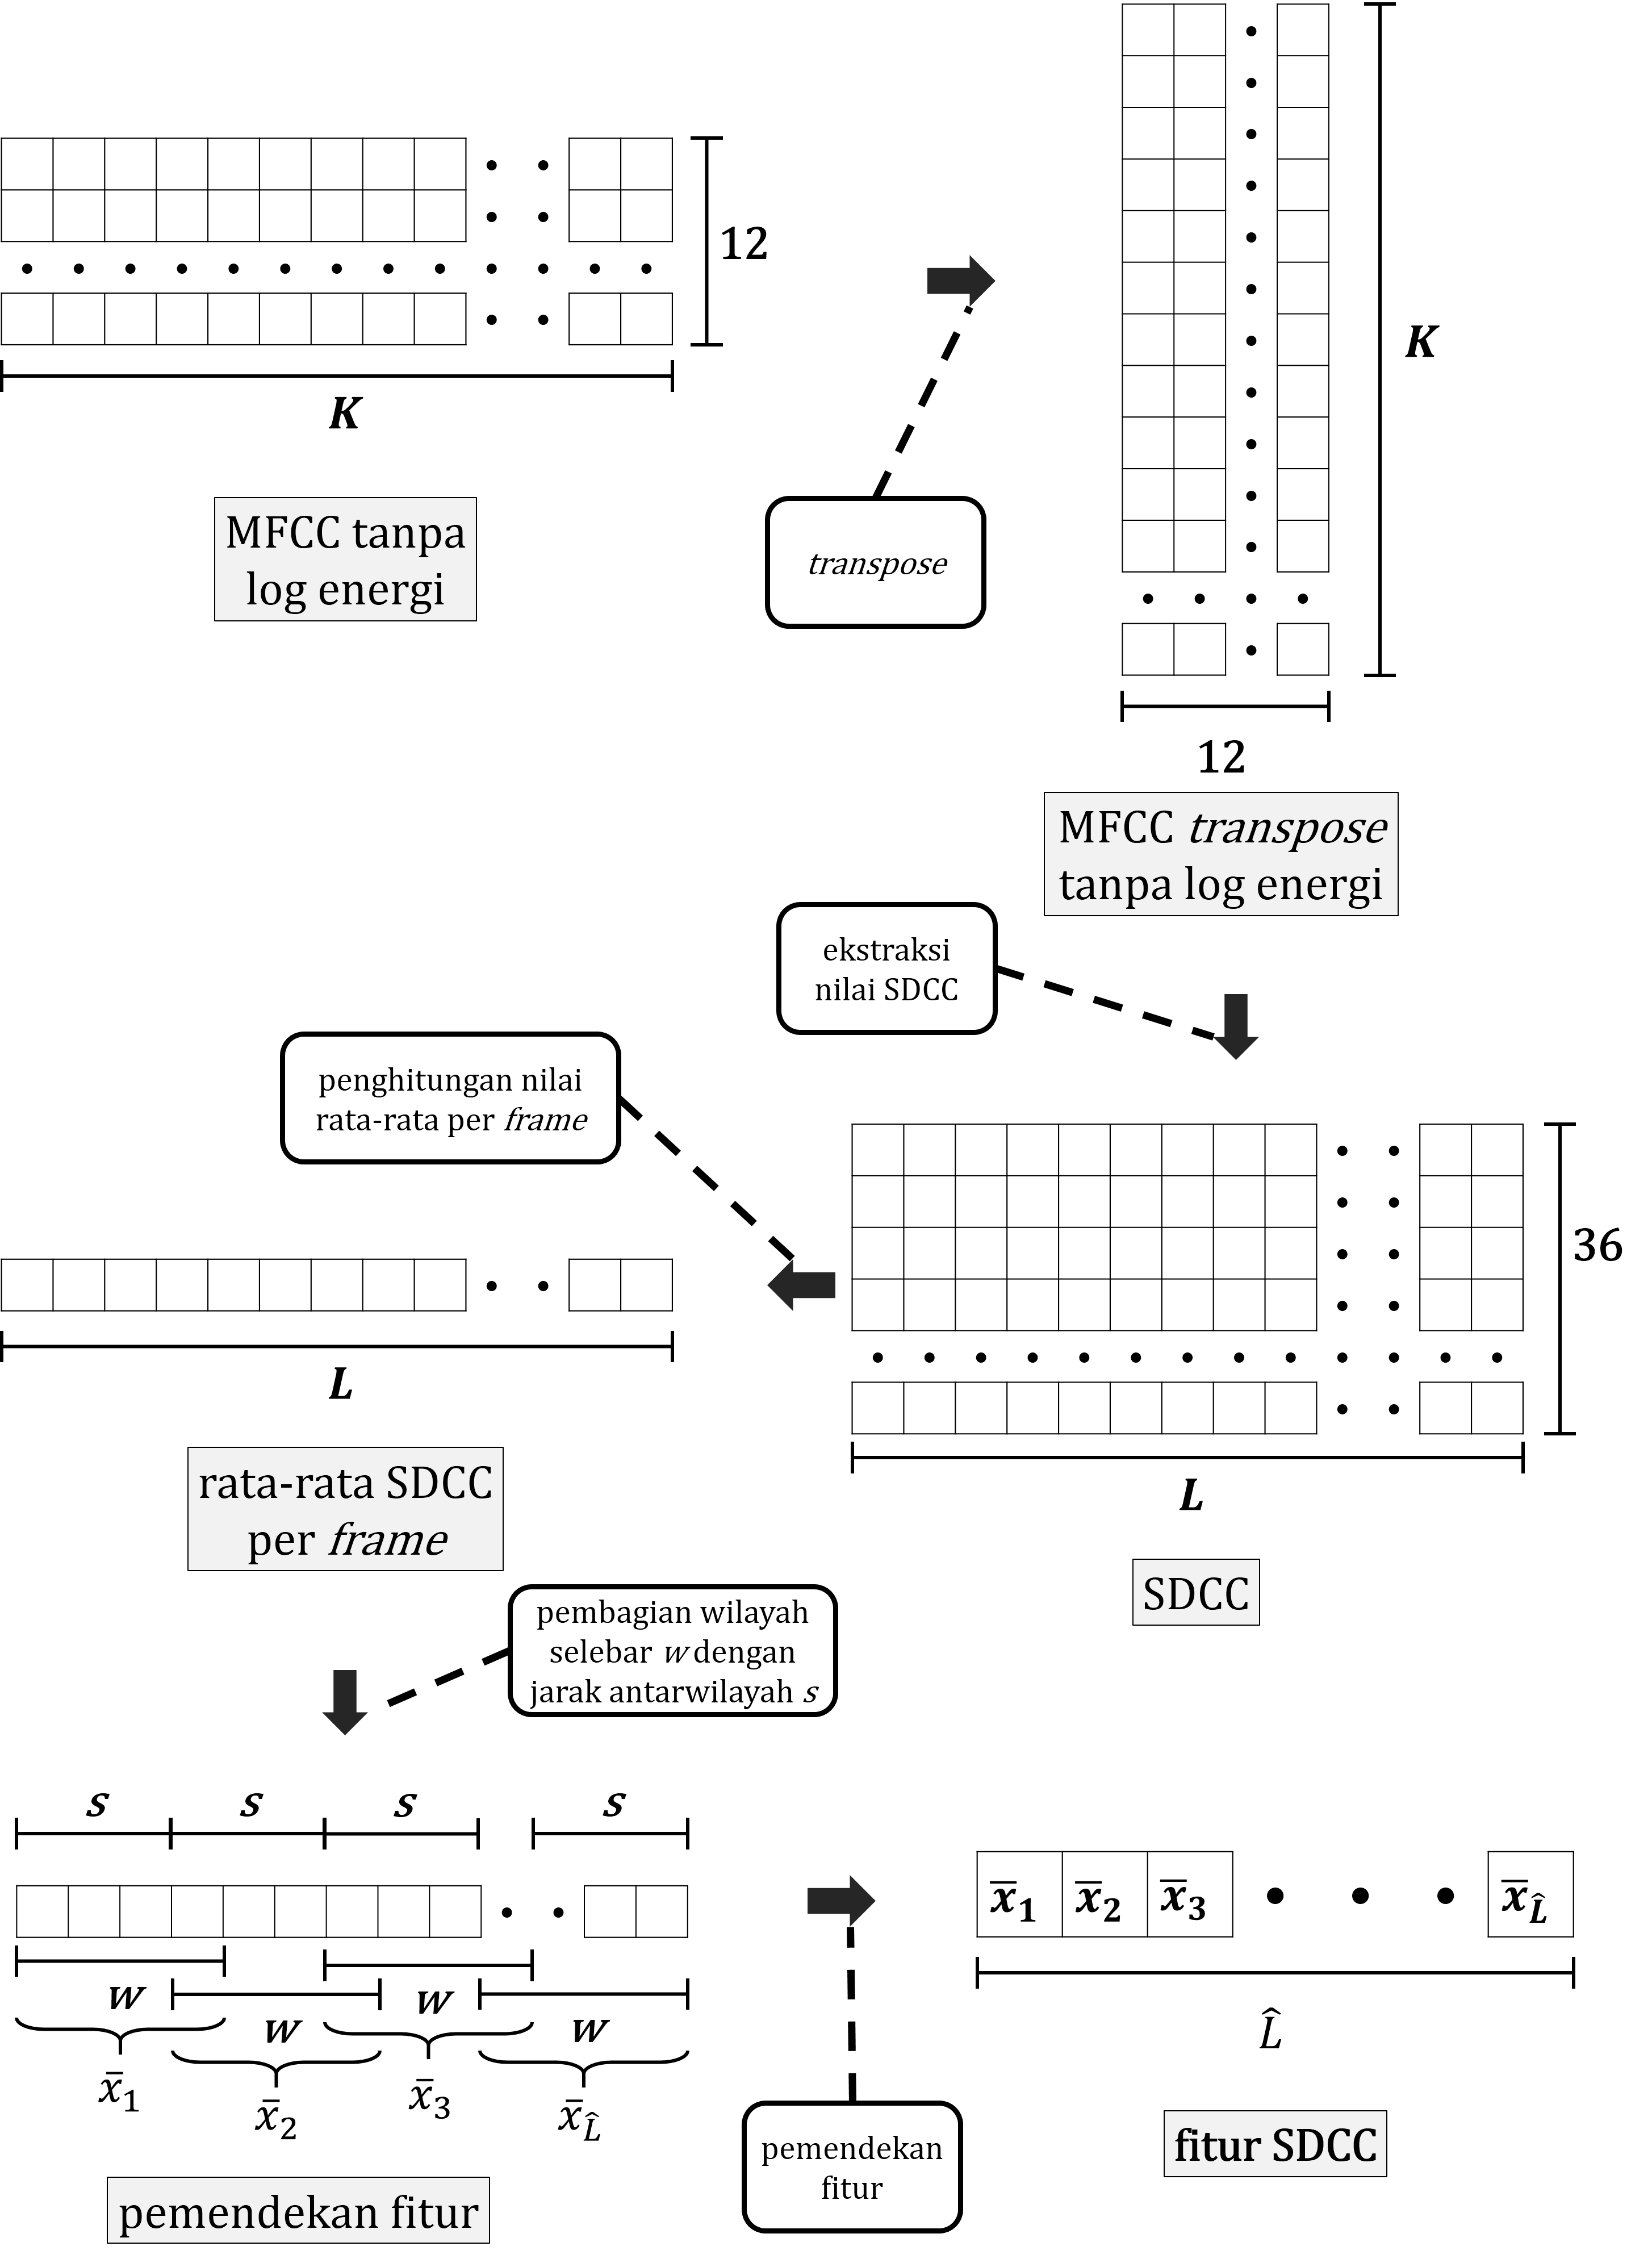
\includegraphics[width=\linewidth]{pics/ekstraksi_sdcc_v2}
    \caption{Alur Ekstraksi Fitur SDCC}
    \label{fig:alurekstraksifitursdcc}
  \end{figure}
\end{enumerate}



\section{Pemodelan} \label{chap:pemodelan}
Penelitian ini menggunakan tiga variasi metode klasifikasi untuk mengenali pola dari fitur-fitur yang dihasilkan melalui proses pada Bab \ref{chap:ekstraksi fitur}, yaitu \f{support vector machine} (SVM), \f{Gaussian mixture model} (GMM), serta gabungan SVM dengan GMM. Satu ayat dari berbagai qari dimodelkan menjadi sebuah model klasifikasi. Ayat-ayat yang sama dari para qari akan dijadikan data sampel dengan label \f{benar}. Ayat-ayat selain ayat tersebut yang tidak mirip secara tekstual akan dijadikan data sampel dengan label \f{salah}. Cara mengetahui dua buat ayat mirip secara tekstual adalah menggunakan pendekatan algoritma \f{dynamic programming} yang sudah dijelaskan pada Bab \ref{lcs}.

	\subsection{Pemodelan dengan Support Vector Machine (SVM)}
	SVM dipilih untuk digunakan dalam eksperimen ini karena memiliki kemampuan yang terbukti kuat dalam melakukan klasifikasi pola. Hal tersebut dijelaskan oleh \cite{campbell2006support} dalam jurnalnya yang berjudul \f{Support Vector Machines for Speaker and Language Recognition}. SVM didasari oleh teori-teori matematika yang kuat, antara lain dengan adalah pemetaan data ke dimensi ruang yang lebih tinggi, pencarian \f{margin} terbesar, dan generalisasi. Alasan lain yang memperkuat penggunaan SVM dalam penelitian ini adalah bahwa SVM merupakan metode klasifikasi dua kelas, sesuai dengan kebutuhan sistem untuk mengklasifikasi data ke dalam dua kelas juga, yaitu kelas \f{benar} dan kelas \f{salah}.

  Metode klasifikasi SVM dalam eksperimen ini menggunakan fungsi MATLAB \f{svmtrain}\footnote{http://www.mathworks.com/help/stats/svmtrain.html} dalam proses pemodelan dan \f{svmclassify}\footnote{http://www.mathworks.com/help/stats/svmclassify.html} dalam proses pengujian, dengan parameter yang dijelaskan pada Tabel \ref{table:parametersvm} berikut.

  \begin{table}
    \centering
    \caption{Parameter SVM dalam Eksperimen}
    \begin{tabular}{|c|c|}
      \hline
      \textbf{Nama Parameter} & \textbf{Nilai Parameter} \\ \hline
      kernel\_function & linear \\ \hline
      method & Sequential Minimal Optimization (SMO) \\ \hline
      MaxIter & 15000 \\ \hline
    \end{tabular}
    \label{table:parametersvm}
  \end{table}



  \subsection{Pemodelan dengan Gaussian Mixture Model (GMM)}
  GMM dipilih dalam eksperimen ini karena banyak penelitian yang menyatakan bahwa GMM dapat memodelkan fitur-fitur \f{speech recognition} dengan baik, salah satunya adalah penelitian yang dilakukan oleh \cite{zahra2013unique}. Ayat-ayat yang berlabel \f{benar} dimodelkan menjadi sebuah GMM, sedangkan ayat-ayat yang berlabel \f{salah} dimodelkan menjadi sebuah GMM lain, sehingga untuk satu ayat terdapat dua GMM yang menjadi model dalam melakukan klasifikasi. Cara menentukan apakah satu data uji masuk ke dalam kelas \f{benar} atau \f{salah} adalah dengan membandingkan nilai PDF dari kedua model tersebut. Jika nilai PDF pada GMM yang memodelkan kelas \f{benar} lebih besar atau sama dengan nilai PDF pada GMM yang memodelkan kelas \f{salah}, maka data uji tersebut diklasifikasikan sebagai data \f{benar}. Selain itu maka data uji tersebut diklasifikasikan sebagai data \f{salah}.

  Metode klasifikasi GMM dalam eksperimen ini menggunakan fungsi MATLAB \f{gmdistribution.fit}\footnote{http://www.mathworks.com/help/stats/gmdistribution.fit.html} dalam proses pemodelan dengan parameter yang dijelaskan pada Tabel \ref{table:parametergmm} berikut.

  \begin{table}
    \centering
    \caption{Parameter GMM dalam Eksperimen}
    \begin{tabular}{|c|c|}
      \hline
      \textbf{Nama Parameter} & \textbf{Nilai Parameter} \\ \hline
      k & 8 \\ \hline
      CovType & diagonal \\ \hline
      SharedCov & true \\ \hline
      MaxIter & 100 \\ \hline
    \end{tabular}
    \label{table:parametergmm}
  \end{table}



  \subsection{Pemodelan dengan Gabungan SVM dan GMM}
	Kemampuan SVM maupun GMM untuk menjadi model sistem ASR sudah teruji baik oleh beberapa penelitian \citep{zahra2013unique}. Maka dalam eksperimen ini dicoba pula gabungan dari dua metode klasifikasi tersebut. Cara menggabungkan dua metode tersebut dalam proses pemodelan adalah sebagai berikut.
	\begin{enumerate}
    \item Buat model pertama, $M_{SVM}$ menggunakan metode klasifikasi SVM dan data sampel.
    \item Buat model kedua, $M_0$ menggunakan GMM dengan sampel data berlabel \f{salah} dan data sampel.
    \item Buat model ketiga, $M_1$ menggunakan GMM dengan sampel data berlabel \f{benar} dan data sampel.
  \end{enumerate}
  Sedangkan cara menggabungkan dua metode tersebut dalam proses pengujian adalah sebagai berikut.
  \begin{enumerate}
    \item Hitung nilai PDF dari data uji pada $M_0$, $P_0$, sebagai nilai probabilitas \f{salah}.
    \item Hitung nilai PDF dari data uji pada $M_1$, $P_1$, sebagai nilai probabilitas \f{benar}.
    \item Klasifikasikan data uji menggunakan metode klasifikasi SVM. dengan model $M_{SVM}$ Jika hasil klasifikasinya bernilai \f{salah}, tambahkan nilai 1 pada $P_0$, dan jika hasil klasifikasinya bernilai \f{benar}, tambahkan nilai 1 pada $P_1$.
    \item Jika nilai $P_1$ lebih besar atau sama dengan $P_0$, maka data uji tersebut diklasifikasikan sebagai data \f{benar}. Selain itu maka data uji tersebut diklasifikasikan sebagai data \f{salah}.
  \end{enumerate}



\section{Pengujian}
Pengujian dilakukan per ayat menggunakan teknik \f{$k$-fold cross validation}, dengan nilai $k$ yang umum digunakan, yaitu $k = 10$. Langkah-langkah dalam melakukan \f{$k$-fold cross validation} adalah sebagai berikut.
\begin{enumerate}
  \item \label{step:pisahkan data} Dari 40 qari yang ada dalam koleksi data eksperimen, gunakan 10\% qari (4 qari) \f{secara acak} sebagai data uji, sedangkan qari-qari lainnya digunakan sebagai data model. Pengacakan tersebut bertujuan untuk membuat proses pengujian menjadi \f{fair} karena tidak ada beberapa qari yang selalu berada kelompok yang sama, baik sebagai kelompok data uji maupun kelompok data model.

  \item \label{step:bangun model} Bangun model sesuai penjelasan pada Bab \ref{chap:pemodelan} menggunakan data model yang diperoleh pada langkah \ref{step:pisahkan data}.

  \item \label{step:klasifikasi} Lakukan proses klasifikasi menggunakan model yang dibangun pada langkah \ref{step:bangun model} terhadap dua kelompok data berikut.
  \begin{enumerate}
    \item Data berlabel \f{benar} diperoleh dari ayat-ayat yang sama. Terdapat 4 \f{instance} berlabel \f{benar} dari 4 qari yang dijadikan data uji.
    \item Data berlabel \f{salah} diperoleh dari ayat-ayat yang tidak mirip secara tekstual. Ambil 4 \f{instance} berlabel \f{salah} secara acak dari 4 qari yang dijadikan data uji.
  \end{enumerate}

  \item \label{step:evaluasi} Lakukan evaluasi terhadap hasil klasifikasi pada langkah \ref{step:klasifikasi}. Evaluasi tersebut akan menghasilkan \f{confusion matrix}, $C$, berukuran $2\times2$ yang merepresentasikan Tabel \ref{table:kontingensi}.

  \item \label{step:ulangi} Ulangi langkah \ref{step:pisahkan data} sampai langkah \ref{step:evaluasi} sebanyak 10 kali. Qari yang sudah menjadi data uji diganti dengan qari lainnya yang belum pernah menjadi data uji. Sehingga seluruh data qari akan mendapat giliran menjadi data uji. Langkah tersebut akan menghasilkan 10 \f{confusion matrix}, $\{C_1, C_2, \dots, C_{10}\}$.

  \item Jumlahkan 10 \f{confusion matrix} yang diperoleh pada langkah \ref{step:ulangi}, sehingga menghasilkan satu \f{confusion matrix} baru, $C_{total} = \sum_{i=1}^{10}{C_i}$. Nilai akurasi, presisi, \f{recall}, serta \f{f-measure} diperoleh dari perhitungan yang sudah dijelaskan pada Bab \ref{chap:evaluasi} dengan mengacu pada matriks $C_{total}$.
\end{enumerate}
%!TEX root = skripsi.tex
%-----------------------------------------------------------------------------%
\chapter{\babLima}
%-----------------------------------------------------------------------------%

Sistem pengenalan suara otomatis pada penelitian ini adalah sistem pengenalan per ayat. Bab \ref{eksperimen} menjelaskan bagaimana eksperimen dilakukan terhadap satu ayat. Setiap ayat mendapat perlakuan sama dalam eksperimen. Pengujian suatu ayat akan menghasilkan sebuah \f{confusion matrix}, lalu dari \f{confusion matrix} diperoleh metrik evaluasi berupa nilai akurasi, presisi, \f{recall}, dan \f{f-measure}. Banyaknya ayat yang diproses dalam eksperimen yang sudah dilakukan adalah 564 ayat, sehingga akan dihasilkan pula 564 metrik evaluasi tersebut.

Untuk menampilkan keseluruhan data hasil eksperimen secara ringkas, data tersebut disajikan dalam bentuk histogram. Sumbu X pada histogram menyatakan interval persentase, sedangkan sumbu Y pada histogram menyatakan banyaknya hasil eksperimen yang berada pada interval tersebut. Contoh interval dalam histogram yang disajikan adalah (90\%,95\%]. Interval tersebut merepresentasikan rentang \f{lebih dari} 90\% dan \f{kurang dari atau sama dengan} 95\%. Semakin tinggi \f{bar} histogram akurasi pada interval (90\%,95\%], artinya semakin banyak ayat yang berhasil diklasifikasikan oleh sistem dengan $90\%<\text{akurasi}\leq95\%$. Jadi jika pada suatu metode, \f{bar} histogram tinggi berkumpul pada interval tinggi, menunjukkan bahwa metode tersebut baik. Sebaliknya, jika \f{bar} histogram tinggi berkumpul pada interval rendah, menunjukkan bahwa metode tersebut kurang baik.

%-----------------------------------------------------------------------------%
\section{Hasil dengan Fitur MFCC}
%-----------------------------------------------------------------------------%

  %-----------------------------------------------------------------------------%
  \subsection{Hasil dengan Fitur MFCC dan Metode Klasifikasi SVM}
  %-----------------------------------------------------------------------------%
  Eksperimen menggunakan fitur MFCC dan menggunakan metode klasifikasi SVM, memberikan hasil yang dirangkum pada Tabel \ref{table:mfccsvm} berikut.

  \begin{table}
    \centering
    \caption{Rangkuman Hasil Eksperimen dengan Fitur MFCC dan Metode Klasifikasi SVM}
    \begin{tabular}{|c|c|c|c|c|}
      \hline
       & Akurasi & Presisi & \f{\f{Recall}} & \f{\f{F-Measure}} \\ \hline
      Minimal         & 41.3\% & 42.2\% & 42.5\% & 44.4\% \\ \hline
      Maksimal        & 87.5\% & 96.2\% & 82.5\% & 86.8\% \\ \hline
      Rata-rata       & 63.1\% & 63.7\% & 63.0\% & 63.1\% \\ \hline
      Standar Deviasi & 0.072  & 0.081  & 0.078  & 0.069  \\ \hline
    \end{tabular}
    \label{table:mfccsvm}
  \end{table}

  Tabel \ref{table:datahistogram00} menunjukkan frekuensi kemunculan persentase tertentu yang dikelompokkan ke dalam interval 5\%.

  \begin{table}
    \centering
    \caption{Frekuensi Kemunculan Interval Persentase pada Eksperimen dengan Fitur MFCC dan Metode Klasifikasi SVM}
    \begin{tabular}{|c|c|c|c|c|}
      \hline
\multicolumn{1}{|c|}{Persentase} & \multicolumn{1}{c|}{\begin{tabular}[c]{@{}c@{}}Frekuensi\\ Nilai Akurasi\end{tabular}} & \multicolumn{1}{c|}{\begin{tabular}[c]{@{}c@{}}Frekuensi\\ Nilai Presisi\end{tabular}} & \multicolumn{1}{c|}{\begin{tabular}[c]{@{}c@{}}Frekuensi\\ Nilai \f{Recall}\end{tabular}} & \multicolumn{1}{c|}{\begin{tabular}[c]{@{}c@{}}Frekuensi\\ Nilai \f{F-Measure}\end{tabular}} \\ \hline
(40\%,45\%{]}  & 6   & 5   & 8   & 2   \\ \hline
(45\%,50\%{]}  & 16  & 17  & 33  & 15  \\ \hline
(50\%,55\%{]}  & 55  & 51  & 67  & 51  \\ \hline
(55\%,60\%{]}  & 120 & 112 & 120 & 114 \\ \hline
(60\%,65\%{]}  & 167 & 148 & 141 & 171 \\ \hline
(65\%,70\%{]}  & 122 & 130 & 121 & 126 \\ \hline
(70\%,75\%{]}  & 52  & 51  & 42  & 58  \\ \hline
(75\%,80\%{]}  & 21  & 30  & 29  & 22  \\ \hline
(80\%,85\%{]}  & 4   & 15  & 3   & 4   \\ \hline
(85\%,90\%{]}  & 1   & 2   & 0   & 1   \\ \hline
(90\%,95\%{]}  & 0   & 2   & 0   & 0   \\ \hline
(95\%,100\%{]} & 0   & 1   & 0   & 0   \\ \hline
    \end{tabular}
    \label{table:datahistogram00}
  \end{table}

  Gambar \ref{fig:histogram00} merepresentasikan Tabel \ref{table:datahistogram00} dalam bentuk histogram.
  \begin{figure}
    \centering
    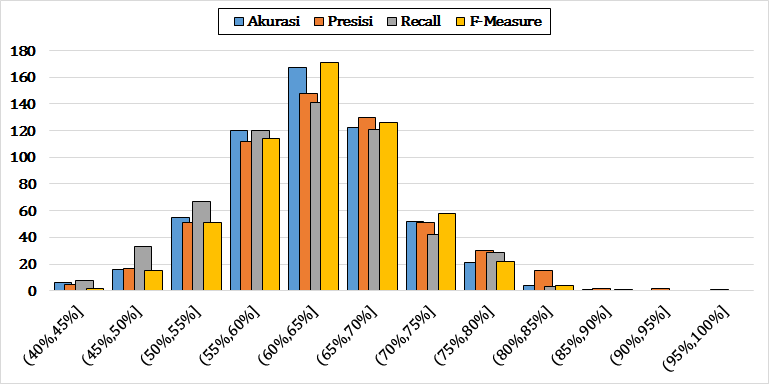
\includegraphics[width=\linewidth]{pics/histogram00}
    \caption{Histogram Metrik Evaluasi dengan Fitur MFCC dan Metode Klasifikasi SVM}
    \label{fig:histogram00}
  \end{figure}

  Dari Gambar \ref{fig:histogram00} dapat diamati bahwa mayoritas ayat dalam eksperimen terklasifikasi dengan rentang akurasi (60\%,65\%].




  %-----------------------------------------------------------------------------%
  \subsection{Hasil dengan Fitur MFCC dan Metode Klasifikasi GMM}
  %-----------------------------------------------------------------------------%
  Eksperimen menggunakan fitur MFCC dan menggunakan metode klasifikasi GMM, memberikan hasil yang dirangkum pada Tabel \ref{table:mfccgmm} berikut.

  \begin{table}
    \centering
    \caption{Rangkuman Hasil Eksperimen dengan Fitur MFCC dan Metode Klasifikasi GMM}
    \begin{tabular}{|c|c|c|c|c|}
      \hline
       & Akurasi & Presisi & \f{\f{Recall}} & \f{\f{F-Measure}} \\ \hline
      Minimal         & 43.8\% & 43.9\% & 42.5\% & 44.4\% \\ \hline
      Maksimal        & 85.0\% & 93.3\% & 90.0\% & 85.0\% \\ \hline
      Rata-rata       & 65.8\% & 66.3\% & 65.1\% & 65.4\% \\ \hline
      Standar Deviasi & 0.065  & 0.072  & 0.086  & 0.067  \\ \hline
    \end{tabular}
    \label{table:mfccgmm}
  \end{table}

  Tabel \ref{table:datahistogram01} menunjukkan frekuensi kemunculan persentase tertentu yang dikelompokkan ke dalam interval 5\%.

  \begin{table}
    \centering
    \caption{Frekuensi Kemunculan Interval Persentase pada Eksperimen dengan Fitur MFCC dan Metode Klasifikasi GMM}
    \begin{tabular}{|c|c|c|c|c|}
      \hline
\multicolumn{1}{|c|}{Persentase} & \multicolumn{1}{c|}{\begin{tabular}[c]{@{}c@{}}Frekuensi\\ Nilai Akurasi\end{tabular}} & \multicolumn{1}{c|}{\begin{tabular}[c]{@{}c@{}}Frekuensi\\ Nilai Presisi\end{tabular}} & \multicolumn{1}{c|}{\begin{tabular}[c]{@{}c@{}}Frekuensi\\ Nilai \f{Recall}\end{tabular}} & \multicolumn{1}{c|}{\begin{tabular}[c]{@{}c@{}}Frekuensi\\ Nilai \f{F-Measure}\end{tabular}} \\ \hline
(40\%,45\%{]}  & 2   & 1   & 6   & 1   \\ \hline
(45\%,50\%{]}  & 3   & 4   & 16  & 7   \\ \hline
(50\%,55\%{]}  & 27  & 21  & 54  & 22  \\ \hline
(55\%,60\%{]}  & 89  & 92  & 115 & 97  \\ \hline
(60\%,65\%{]}  & 144 & 116 & 137 & 146 \\ \hline
(65\%,70\%{]}  & 169 & 181 & 111 & 151 \\ \hline
(70\%,75\%{]}  & 94  & 91  & 63  & 95  \\ \hline
(75\%,80\%{]}  & 31  & 38  & 37  & 40  \\ \hline
(80\%,85\%{]}  & 5   & 15  & 19  & 5   \\ \hline
(85\%,90\%{]}  & 0   & 4   & 6   & 0   \\ \hline
(90\%,95\%{]}  & 0   & 1   & 0   & 0   \\ \hline
(95\%,100\%{]} & 0   & 0   & 0   & 0   \\ \hline
    \end{tabular}
    \label{table:datahistogram01}
  \end{table}
  
  Gambar \ref{fig:histogram01} merepresentasikan Tabel \ref{table:datahistogram01} dalam bentuk histogram.
  \begin{figure}
    \centering
    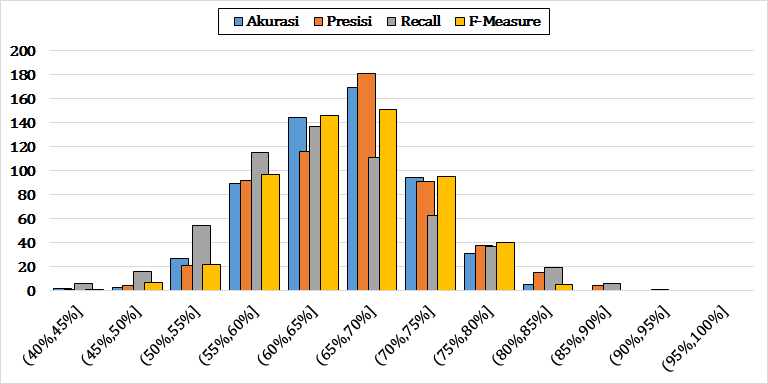
\includegraphics[width=\linewidth]{pics/histogram01}
    \caption{Histogram Metrik Evaluasi dengan Fitur MFCC dan Metode Klasifikasi GMM}
    \label{fig:histogram01}
  \end{figure}

  Dari Gambar \ref{fig:histogram01} dapat diamati bahwa mayoritas ayat dalam eksperimen terklasifikasi dengan rentang akurasi (65\%,70\%]. Hasil tersebut sedikit lebih tinggi jika dibandingkan dengan hasil pada eksperimen yang menggunakan fitur MFCC dan metode klasifikasi SVM. Hal itu mengindikasikan bahwa metode klasifikasi GMM lebih tepat untuk digunakan dalam sistem evaluasi pembacaan \quran~dalam penelitian ini.

  %-----------------------------------------------------------------------------%
  \subsection{Hasil dengan Fitur MFCC dan Metode Klasifikasi Gabungan}
  %-----------------------------------------------------------------------------%
  Eksperimen menggunakan fitur MFCC dengan metode klasifikasi gabungan antara SVM dan GMM, memberikan hasil yang dirangkum pada Tabel \ref{table:mfccgabungan} berikut.

  \begin{table}
    \centering
    \caption{Rangkuman Hasil Eksperimen dengan Fitur MFCC dan Metode Klasifikasi Gabungan}
    \begin{tabular}{|c|c|c|c|c|}
      \hline
       & Akurasi & Presisi & \f{\f{Recall}} & \f{\f{F-Measure}} \\ \hline
      Minimal         & 41.3\% & 42.2\% & 37.5\% & 43.9\% \\ \hline
      Maksimal        & 85.0\% & 90.0\% & 85.0\% & 84.2\% \\ \hline
      Rata-rata       & 63.5\% & 64.1\% & 63.1\% & 63.4\% \\ \hline
      Standar Deviasi & 0.076  & 0.087  & 0.080  & 0.073  \\ \hline
    \end{tabular}
    \label{table:mfccgabungan}
  \end{table}

  Tabel \ref{table:datahistogram02} menunjukkan frekuensi kemunculan persentase tertentu yang dikelompokkan ke dalam interval 5\%.

  \begin{table}
    \centering
    \caption{Frekuensi Kemunculan Interval Persentase pada Eksperimen dengan Fitur MFCC dan Metode Klasifikasi Gabungan}
    \begin{tabular}{|c|c|c|c|c|}
      \hline
\multicolumn{1}{|c|}{Persentase} & \multicolumn{1}{c|}{\begin{tabular}[c]{@{}c@{}}Frekuensi\\ Nilai Akurasi\end{tabular}} & \multicolumn{1}{c|}{\begin{tabular}[c]{@{}c@{}}Frekuensi\\ Nilai Presisi\end{tabular}} & \multicolumn{1}{c|}{\begin{tabular}[c]{@{}c@{}}Frekuensi\\ Nilai \f{Recall}\end{tabular}} & \multicolumn{1}{c|}{\begin{tabular}[c]{@{}c@{}}Frekuensi\\ Nilai \f{F-Measure}\end{tabular}} \\ \hline
(40\%,45\%{]}  & 5   & 3   & 10  & 4   \\ \hline
(45\%,50\%{]}  & 19  & 21  & 25  & 14  \\ \hline
(50\%,55\%{]}  & 64  & 60  & 84  & 57  \\ \hline
(55\%,60\%{]}  & 115 & 116 & 109 & 116 \\ \hline
(60\%,65\%{]}  & 145 & 128 & 132 & 143 \\ \hline
(65\%,70\%{]}  & 104 & 100 & 119 & 119 \\ \hline
(70\%,75\%{]}  & 83  & 73  & 55  & 85  \\ \hline
(75\%,80\%{]}  & 24  & 39  & 26  & 21  \\ \hline
(80\%,85\%{]}  & 5   & 16  & 4   & 5   \\ \hline
(85\%,90\%{]}  & 0   & 8   & 0   & 0   \\ \hline
(90\%,95\%{]}  & 0   & 0   & 0   & 0   \\ \hline
(95\%,100\%{]} & 0   & 0   & 0   & 0   \\ \hline
    \end{tabular}
    \label{table:datahistogram02}
  \end{table}
  
  Gambar \ref{fig:histogram02} merepresentasikan Tabel \ref{table:datahistogram02} dalam bentuk histogram.
  \begin{figure}
    \centering
    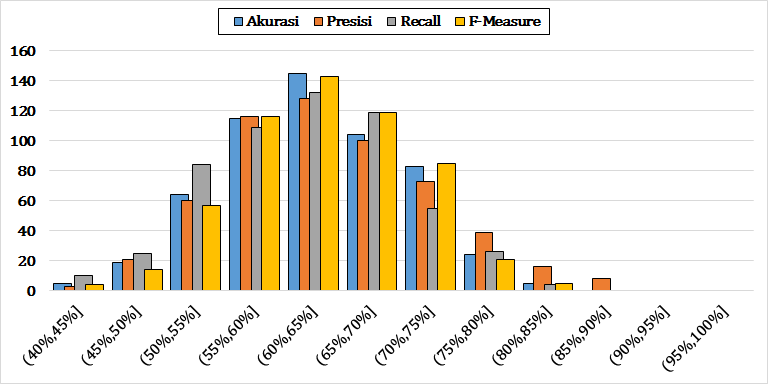
\includegraphics[width=\linewidth]{pics/histogram02}
    \caption{Histogram Metrik Evaluasi dengan Fitur MFCC dan Metode Klasifikasi Gabungan}
    \label{fig:histogram02}
  \end{figure}

  Dari Gambar \ref{fig:histogram02} dapat diamati bahwa mayoritas ayat dalam eksperimen terklasifikasi dengan rentang akurasi (60\%,65\%]. Hasil tersebut sedikit lebih rendah jika dibandingkan dengan hasil pada eksperimen yang menggunakan fitur MFCC dan metode klasifikasi GMM. Hal itu mengindikasikan bahwa gabungan dua metode klasifikasi, yaitu SVM dengan GMM, tidak lebih tepat untuk digunakan dalam sistem evaluasi pembacaan \quran~dalam eksperimen ini jika dibandingkan dengan metode klasifikasi GMM.





%-----------------------------------------------------------------------------%
\section{Hasil dengan Fitur SDCC}
%-----------------------------------------------------------------------------%

  %-----------------------------------------------------------------------------%
  \subsection{Hasil dengan Fitur SDCC dan Metode Klasifikasi SVM}
  %-----------------------------------------------------------------------------%
  Eksperimen menggunakan fitur SDCC dan menggunakan metode klasifikasi SVM, memberikan hasil yang dirangkum pada Tabel \ref{table:sdccsvm} berikut.

  \begin{table}
    \centering
    \caption{Rangkuman Hasil Eksperimen dengan Fitur SDCC dan Metode Klasifikasi SVM}
    \begin{tabular}{|c|c|c|c|c|}
      \hline
       & Akurasi & Presisi & \f{\f{Recall}} & \f{\f{F-Measure}} \\ \hline
      Minimal         & 51.3\% & 51.2\%  & 30.0\%  & 43.6\% \\ \hline
      Maksimal        & 96.3\% & 100.0\% & 100.0\% & 96.4\% \\ \hline
      Rata-rata       & 77.3\% & 76.6\%  & 79.5\%  & 77.8\% \\ \hline
      Standar Deviasi & 0.075  & 0.082   & 0.087   & 0.074  \\ \hline
    \end{tabular}
    \label{table:sdccsvm}
  \end{table}

  Tabel \ref{table:datahistogram10} menunjukkan frekuensi kemunculan persentase tertentu yang dikelompokkan ke dalam interval 5\%.

  \begin{table}
    \centering
    \caption{Frekuensi Kemunculan Interval Persentase pada Eksperimen dengan Fitur SDCC dan Metode Klasifikasi SVM}
    \begin{tabular}{|c|c|c|c|c|}
      \hline
\multicolumn{1}{|c|}{Persentase} & \multicolumn{1}{c|}{\begin{tabular}[c]{@{}c@{}}Frekuensi\\ Nilai Akurasi\end{tabular}} & \multicolumn{1}{c|}{\begin{tabular}[c]{@{}c@{}}Frekuensi\\ Nilai Presisi\end{tabular}} & \multicolumn{1}{c|}{\begin{tabular}[c]{@{}c@{}}Frekuensi\\ Nilai \f{Recall}\end{tabular}} & \multicolumn{1}{c|}{\begin{tabular}[c]{@{}c@{}}Frekuensi\\ Nilai \f{F-Measure}\end{tabular}} \\ \hline
(40\%,45\%{]}  & 0   & 0   & 3   & 1   \\ \hline
(45\%,50\%{]}  & 0   & 0   & 1   & 1   \\ \hline
(50\%,55\%{]}  & 2   & 2   & 6   & 1   \\ \hline
(55\%,60\%{]}  & 3   & 8   & 6   & 4   \\ \hline
(60\%,65\%{]}  & 28  & 25  & 14  & 16  \\ \hline
(65\%,70\%{]}  & 73  & 96  & 44  & 65  \\ \hline
(70\%,75\%{]}  & 129 & 122 & 113 & 117 \\ \hline
(75\%,80\%{]}  & 132 & 132 & 131 & 142 \\ \hline
(80\%,85\%{]}  & 120 & 93  & 120 & 136 \\ \hline
(85\%,90\%{]}  & 58  & 55  & 86  & 57  \\ \hline
(90\%,95\%{]}  & 17  & 25  & 35  & 22  \\ \hline
(95\%,100\%{]} & 2   & 6   & 5   & 2   \\ \hline
    \end{tabular}
    \label{table:datahistogram10}
  \end{table}
  
  Gambar \ref{fig:histogram10} merepresentasikan Tabel \ref{table:datahistogram10} dalam bentuk histogram.
  \begin{figure}
    \centering
    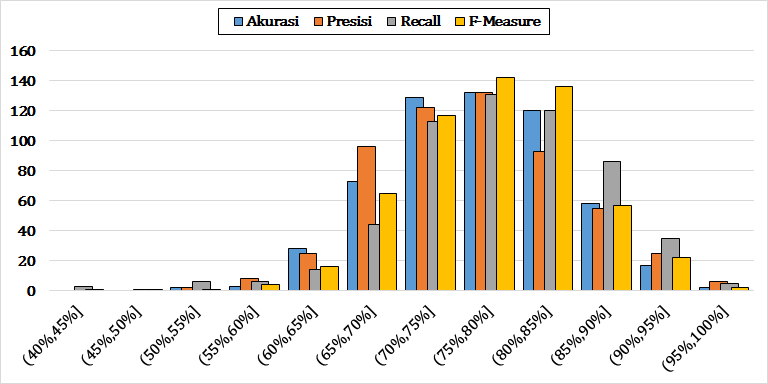
\includegraphics[width=\linewidth]{pics/histogram10}
    \caption{Histogram Metrik Evaluasi dengan Fitur SDCC dan Metode Klasifikasi SVM}
    \label{fig:histogram10}
  \end{figure}

  Dari Gambar \ref{fig:histogram10} dapat diamati bahwa mayoritas ayat dalam eksperimen terklasifikasi dengan rentang akurasi (75\%,80\%]. Hasil tersebut secara signifikan lebih tinggi jika dibandingkan dengan beberapa hasil pada eksperimen yang menggunakan fitur MFCC. Hal itu mengindikasikan bahwa penggunaan fitur SDCC lebih tepat daripada fitur MFCC, untuk digunakan dalam sistem evaluasi pembacaan \quran~dalam penelitian ini.





  %-----------------------------------------------------------------------------%
  \subsection{Hasil dengan Fitur SDCC dan Metode Klasifikasi GMM}
  %-----------------------------------------------------------------------------%
  Eksperimen menggunakan fitur SDCC dan menggunakan metode klasifikasi GMM, memberikan hasil yang dirangkum pada Tabel \ref{table:sdccgmm} berikut.

  \begin{table}
    \centering
    \caption{Rangkuman Hasil Eksperimen dengan Fitur SDCC dan Metode Klasifikasi SVM}
    \begin{tabular}{|c|c|c|c|c|}
      \hline
       & Akurasi & Presisi & \f{\f{Recall}} & \f{\f{F-Measure}} \\ \hline
      Minimal         & 67.5\% & 64.6\%  & 55.0\%  & 63.8\% \\ \hline
      Maksimal        & 98.8\% & 100.0\% & 100.0\% & 98.8\% \\ \hline
      Rata-rata       & 83.4\% & 89.0\%  & 76.4\%  & 82.0\% \\ \hline
      Standar Deviasi & 0.056  & 0.064   & 0.082   & 0.063  \\ \hline
    \end{tabular}
    \label{table:sdccgmm}
  \end{table}

  Tabel \ref{table:datahistogram11} menunjukkan frekuensi kemunculan persentase tertentu yang dikelompokkan ke dalam interval 5\%.

  \begin{table}
    \centering
    \caption{Frekuensi Kemunculan Interval Persentase pada Eksperimen dengan Fitur SDCC dan Metode Klasifikasi GMM}
    \begin{tabular}{|c|c|c|c|c|}
      \hline
\multicolumn{1}{|c|}{Persentase} & \multicolumn{1}{c|}{\begin{tabular}[c]{@{}c@{}}Frekuensi\\ Nilai Akurasi\end{tabular}} & \multicolumn{1}{c|}{\begin{tabular}[c]{@{}c@{}}Frekuensi\\ Nilai Presisi\end{tabular}} & \multicolumn{1}{c|}{\begin{tabular}[c]{@{}c@{}}Frekuensi\\ Nilai \f{Recall}\end{tabular}} & \multicolumn{1}{c|}{\begin{tabular}[c]{@{}c@{}}Frekuensi\\ Nilai \f{F-Measure}\end{tabular}} \\ \hline
(40\%,45\%{]}  & 0   & 0   & 0   & 0   \\ \hline
(45\%,50\%{]}  & 0   & 0   & 0   & 0   \\ \hline
(50\%,55\%{]}  & 0   & 0   & 3   & 0   \\ \hline
(55\%,60\%{]}  & 0   & 0   & 11  & 0   \\ \hline
(60\%,65\%{]}  & 0   & 1   & 45  & 5   \\ \hline
(65\%,70\%{]}  & 10  & 1   & 94  & 12  \\ \hline
(70\%,75\%{]}  & 36  & 10  & 130 & 56  \\ \hline
(75\%,80\%{]}  & 128 & 41  & 129 & 141 \\ \hline
(80\%,85\%{]}  & 193 & 96  & 83  & 171 \\ \hline
(85\%,90\%{]}  & 138 & 161 & 48  & 119 \\ \hline
(90\%,95\%{]}  & 53  & 155 & 18  & 54  \\ \hline
(95\%,100\%{]} & 6   & 99  & 3   & 6   \\ \hline
    \end{tabular}
    \label{table:datahistogram11}
  \end{table}
  
  Gambar \ref{fig:histogram11} merepresentasikan Tabel \ref{table:datahistogram11} dalam bentuk histogram.
  \begin{figure}
    \centering
    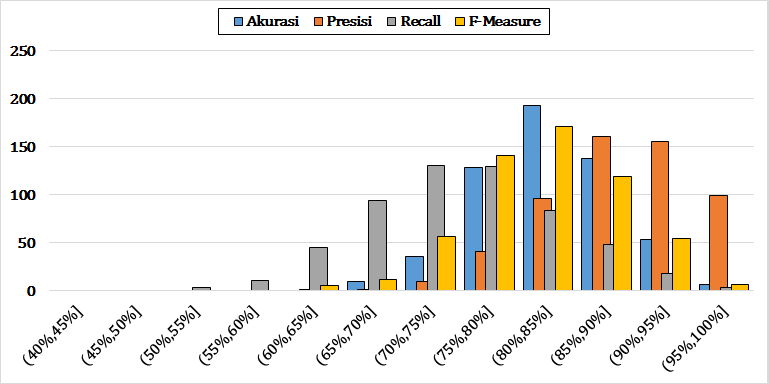
\includegraphics[width=\linewidth]{pics/histogram11}
    \caption{Histogram Metrik Evaluasi dengan Fitur SDCC dan Metode Klasifikasi GMM}
    \label{fig:histogram11}
  \end{figure}

  Dari Gambar \ref{fig:histogram11} dapat diamati bahwa mayoritas ayat dalam eksperimen terklasifikasi dengan rentang akurasi (80\%,85\%]. Hasil tersebut sedikit lebih tinggi jika dibandingkan dengan hasil pada eksperimen yang menggunakan fitur SDCC dan metode klasifikasi SVM. Hal itu semakin mengindikasikan bahwa metode klasifikasi GMM lebih tepat untuk digunakan dalam sistem evaluasi pembacaan \quran~dalam eksperimen ini.






  %-----------------------------------------------------------------------------%
  \subsection{Hasil dengan Fitur SDCC dan Metode Klasifikasi Gabungan}
  %-----------------------------------------------------------------------------%
  Eksperimen menggunakan fitur SDCC dan menggunakan metode klasifikasi gabungan SVM dengan GMM, memberikan hasil yang dirangkum pada Tabel \ref{table:sdccgabungan} berikut.

  \begin{table}
    \centering
    \caption{Rangkuman Hasil Eksperimen dengan Fitur SDCC dan Metode Klasifikasi SVM}
    \begin{tabular}{|c|c|c|c|c|}
      \hline
       & Akurasi & Presisi & \f{\f{Recall}} & \f{\f{F-Measure}} \\ \hline
      Minimal         & 57.5\% & 56.5\%  & 65.0\%  & 60.5\% \\ \hline
      Maksimal        & 96.3\% & 100.0\% & 100.0\% & 96.4\% \\ \hline
      Rata-rata       & 79.4\% & 77.3\%  & 84.2\%  & 80.4\% \\ \hline
      Standar Deviasi & 0.069  & 0.078   & 0.065   & 0.062  \\ \hline
    \end{tabular}
    \label{table:sdccgabungan}
  \end{table}

  Tabel \ref{table:datahistogram12} menunjukkan frekuensi kemunculan persentase tertentu yang dikelompokkan ke dalam interval 5\%.

  \begin{table}
    \centering
    \caption{Frekuensi Kemunculan Interval Persentase pada Eksperimen dengan Fitur SDCC dan Metode Klasifikasi Gabungan}
    \begin{tabular}{|c|c|c|c|c|}
      \hline
\multicolumn{1}{|c|}{Persentase} & \multicolumn{1}{c|}{\begin{tabular}[c]{@{}c@{}}Frekuensi\\ Nilai Akurasi\end{tabular}} & \multicolumn{1}{c|}{\begin{tabular}[c]{@{}c@{}}Frekuensi\\ Nilai Presisi\end{tabular}} & \multicolumn{1}{c|}{\begin{tabular}[c]{@{}c@{}}Frekuensi\\ Nilai \f{Recall}\end{tabular}} & \multicolumn{1}{c|}{\begin{tabular}[c]{@{}c@{}}Frekuensi\\ Nilai \f{F-Measure}\end{tabular}} \\ \hline
(40\%,45\%{]}  & 0   & 0   & 0   & 0   \\ \hline
(45\%,50\%{]}  & 0   & 0   & 0   & 0   \\ \hline
(50\%,55\%{]}  & 0   & 0   & 0   & 0   \\ \hline
(55\%,60\%{]}  & 2   & 6   & 0   & 0   \\ \hline
(60\%,65\%{]}  & 13  & 23  & 3   & 2   \\ \hline
(65\%,70\%{]}  & 49  & 76  & 14  & 26  \\ \hline
(70\%,75\%{]}  & 96  & 123 & 47  & 80  \\ \hline
(75\%,80\%{]}  & 161 & 144 & 119 & 171 \\ \hline
(80\%,85\%{]}  & 137 & 98  & 152 & 154 \\ \hline
(85\%,90\%{]}  & 83  & 60  & 150 & 98  \\ \hline
(90\%,95\%{]}  & 21  & 29  & 71  & 29  \\ \hline
(95\%,100\%{]} & 2   & 5   & 8   & 4   \\ \hline
    \end{tabular}
    \label{table:datahistogram12}
  \end{table}

  Gambar \ref{fig:histogram12} merepresentasikan Tabel \ref{table:datahistogram12} dalam bentuk histogram.
  \begin{figure}
    \centering
    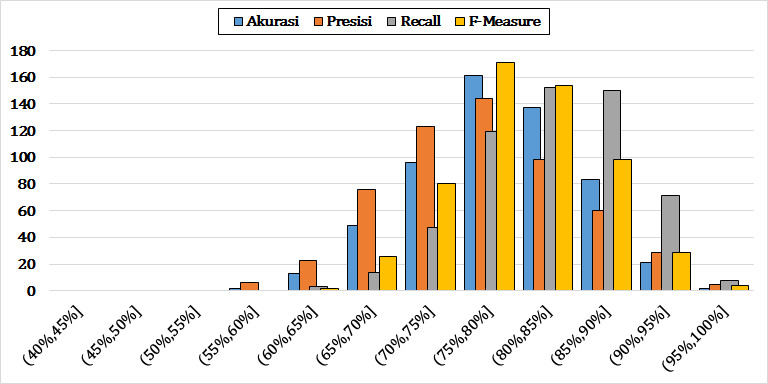
\includegraphics[width=\linewidth]{pics/histogram12}
    \caption{Histogram Metrik Evaluasi dengan Fitur SDCC dan Metode Klasifikasi Gabungan}
    \label{fig:histogram12}
  \end{figure}

  Dari Gambar \ref{fig:histogram12} dapat diamati bahwa mayoritas ayat dalam eksperimen terklasifikasi dengan rentang akurasi (75\%,80\%]. Hasil tersebut sedikit lebih rendah jika dibandingkan dengan hasil pada eksperimen yang menggunakan fitur SDCC dan metode klasifikasi GMM. Hal itu semakin mengindikasikan bahwa gabungan dua metode klasifikasi, yaitu SVM dengan GMM, tidak lebih tepat untuk digunakan dalam sistem evaluasi pembacaan \quran~dalam eksperimen ini jika dibandingkan dengan metode klasifikasi GMM.

















%-----------------------------------------------------------------------------%
\section{Perbandingan Hasil}
%-----------------------------------------------------------------------------%

  %-----------------------------------------------------------------------------%
  \subsection{Perbandingan Metode Klasifikasi pada Fitur MFCC}
  %-----------------------------------------------------------------------------%
  Eksperimen menggunakan fitur MFCC dengan berbagai metode klasifikasi, memberikan hasil yang nilai akurasinya dirangkum pada Tabel \ref{table:perbandinganmfcc} berikut.
  
  \begin{table}
    \centering
    \caption{Perbandingan Hasil Eksperimen dengan Fitur MFCC}
    \begin{tabular}{|c|c|c|c|}
      \hline
       & Akurasi SVM & Akurasi GMM & Akurasi Gabungan \\ \hline
      Minimal         & 41.3\% & 43.8\% & 41.3\% \\ \hline
      Maksimal        & 87.5\% & 85.0\% & 85.0\% \\ \hline
      Rata-rata       & 63.1\% & 65.8\% & 63.5\% \\ \hline
      Standar Deviasi & 0.072  & 0.065  & 0.076  \\ \hline
    \end{tabular}
    \label{table:perbandinganmfcc}
  \end{table}

  Tabel \ref{table:datahistogramakurasimfcc} menunjukkan frekuensi kemunculan persentase tertentu yang dikelompokkan ke dalam interval 5\%.
  \begin{table}
    \centering
    \caption{Frekuensi Kemunculan Interval Persentase pada Eksperimen dengan Fitur MFCC}
    \begin{tabular}{|c|c|c|c|}
      \hline
\multicolumn{1}{|c|}{Persentase} & \multicolumn{1}{c|}{\begin{tabular}[c]{@{}c@{}}Frekuensi Nilai\\ Akurasi SVM\end{tabular}} & \multicolumn{1}{c|}{\begin{tabular}[c]{@{}c@{}}Frekuensi Nilai\\ Akurasi GMM\end{tabular}} & \multicolumn{1}{c|}{\begin{tabular}[c]{@{}c@{}}Frekuensi Nilai\\ Akurasi Gabungan\end{tabular}} \\ \hline
(40\%,45\%{]}  & 6   & 2   & 5   \\ \hline
(45\%,50\%{]}  & 16  & 3   & 19  \\ \hline
(50\%,55\%{]}  & 55  & 27  & 64  \\ \hline
(55\%,60\%{]}  & 120 & 89  & 115 \\ \hline
(60\%,65\%{]}  & 167 & 144 & 145 \\ \hline
(65\%,70\%{]}  & 122 & 169 & 104 \\ \hline
(70\%,75\%{]}  & 52  & 94  & 83  \\ \hline
(75\%,80\%{]}  & 21  & 31  & 24  \\ \hline
(80\%,85\%{]}  & 4   & 5   & 5   \\ \hline
(85\%,90\%{]}  & 1   & 0   & 0   \\ \hline
(90\%,95\%{]}  & 0   & 0   & 0   \\ \hline
(95\%,100\%{]} & 0   & 0   & 0   \\ \hline
    \end{tabular}
    \label{table:datahistogramakurasimfcc}
  \end{table}

  Gambar \ref{fig:histogramakurasimfcc} merepresentasikan Tabel \ref{table:datahistogramakurasimfcc} dalam bentuk histogram.
  \begin{figure}
    \centering
    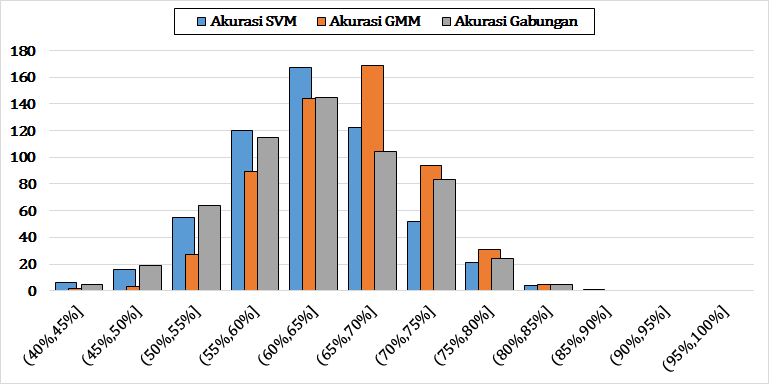
\includegraphics[width=\linewidth]{pics/histogram_akurasi_mfcc}
    \caption{Histogram Akurasi dengan Fitur MFCC}
    \label{fig:histogramakurasimfcc}
  \end{figure}

  Berdasarkan Gambar \ref{table:datahistogramakurasimfcc}, metode klasifikasi GMM mendominasi akurasi pada interval yang lebih tinggi jika dibandingkan dengan dua metode klasifikasi lainnya, walaupun tidak signifikan.



  %-----------------------------------------------------------------------------%
  \subsection{Perbandingan Metode Klasifikasi pada Fitur SDCC}
  %-----------------------------------------------------------------------------%
  Eksperimen menggunakan fitur SDCC dengan berbagai metode klasifikasi, memberikan hasil yang nilai akurasinya dirangkum pada Tabel \ref{table:perbandingansdcc} berikut.

  \begin{table}
    \centering
    \caption{Perbandingan Hasil Eksperimen dengan Fitur SDCC}
    \begin{tabular}{|c|c|c|c|}
      \hline
       & Akurasi SVM & Akurasi GMM & Akurasi Gabungan \\ \hline
      Minimal         & 51.3\% & 67.5\% & 57.5\% \\ \hline
      Maksimal        & 96.3\% & 98.8\% & 96.3\% \\ \hline
      Rata-rata       & 77.3\% & 83.4\% & 79.4\% \\ \hline
      Standar Deviasi & 0.075  & 0.056  & 0.069  \\ \hline
    \end{tabular}
    \label{table:perbandingansdcc}
  \end{table}

  Tabel \ref{table:datahistogramakurasisdcc} menunjukkan frekuensi kemunculan persentase tertentu yang dikelompokkan ke dalam interval 5\%.
  \begin{table}
    \centering
    \caption{Frekuensi Kemunculan Interval Persentase pada Eksperimen dengan Fitur SDCC}
    \begin{tabular}{|c|c|c|c|}
      \hline
\multicolumn{1}{|c|}{Persentase} & \multicolumn{1}{c|}{\begin{tabular}[c]{@{}c@{}}Frekuensi Nilai\\ Akurasi SVM\end{tabular}} & \multicolumn{1}{c|}{\begin{tabular}[c]{@{}c@{}}Frekuensi Nilai\\ Akurasi GMM\end{tabular}} & \multicolumn{1}{c|}{\begin{tabular}[c]{@{}c@{}}Frekuensi Nilai\\ Akurasi Gabungan\end{tabular}} \\ \hline
(40\%,45\%{]}  & 0   & 0   & 0   \\ \hline
(45\%,50\%{]}  & 0   & 0   & 0   \\ \hline
(50\%,55\%{]}  & 2   & 0   & 0   \\ \hline
(55\%,60\%{]}  & 3   & 0   & 2   \\ \hline
(60\%,65\%{]}  & 28  & 0   & 13  \\ \hline
(65\%,70\%{]}  & 73  & 10  & 49  \\ \hline
(70\%,75\%{]}  & 129 & 36  & 96  \\ \hline
(75\%,80\%{]}  & 132 & 128 & 161 \\ \hline
(80\%,85\%{]}  & 120 & 193 & 137 \\ \hline
(85\%,90\%{]}  & 58  & 138 & 83  \\ \hline
(90\%,95\%{]}  & 17  & 53  & 21  \\ \hline
(95\%,100\%{]} & 2   & 6   & 2   \\ \hline
    \end{tabular}
    \label{table:datahistogramakurasisdcc}
  \end{table}

  Gambar \ref{fig:histogramakurasisdcc} merepresentasikan Tabel \ref{table:datahistogramakurasisdcc} dalam bentuk histogram.
  \begin{figure}
    \centering
    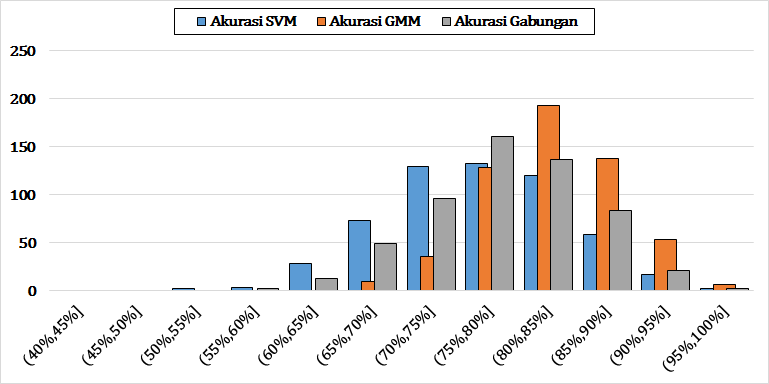
\includegraphics[width=\linewidth]{pics/histogram_akurasi_sdcc}
    \caption{Histogram Akurasi dengan Fitur SDCC}
    \label{fig:histogramakurasisdcc}
  \end{figure}

  Berdasarkan Gambar \ref{table:datahistogramakurasisdcc}, metode klasifikasi GMM mendominasi akurasi pada interval yang lebih tinggi jika dibandingkan dengan dua metode klasifikasi lainnya, dan perbedaannya terlihat secara signifikan. Hal itu semakin memperkuat pernyataan bahwa metode klasifikasi GMM lebih tepat untuk digunakan dalam sistem ini daripada dua metode klasifikasi lainnya.

  







  %-----------------------------------------------------------------------------%
  \subsection{Perbandingan Fitur pada Metode Klasifikasi SVM}
  %-----------------------------------------------------------------------------%
  Eksperimen yang menggunakan metode klasifikasi SVM dengan berbagai pengambilan fitur, memberikan hasil yang nilai akurasinya dirangkum pada Tabel \ref{table:perbandingansvm} berikut.

  \begin{table}
    \centering
    \caption{Perbandingan Hasil Eksperimen dengan Metode Klasifikasi SVM}
    \begin{tabular}{|c|c|c|}
      \hline
       & Akurasi MFCC & Akurasi SDCC \\ \hline
      Minimal         & 41.3\% & 51.3\% \\ \hline
      Maksimal        & 87.5\% & 96.3\% \\ \hline
      Rata-rata       & 63.1\% & 77.3\% \\ \hline
      Standar Deviasi & 0.072  & 0.075  \\ \hline
    \end{tabular}
    \label{table:perbandingansvm}
  \end{table}

  Tabel \ref{table:datahistogramakurasisvm} menunjukkan frekuensi kemunculan persentase tertentu yang dikelompokkan ke dalam interval 5\%.
  \begin{table}
    \centering
    \caption{Frekuensi Kemunculan Interval Persentase pada Eksperimen dengan Metode Klasifikasi SVM}
    \begin{tabular}{|c|c|c|}
      \hline
\multicolumn{1}{|c|}{Persentase} & \multicolumn{1}{c|}{\begin{tabular}[c]{@{}c@{}}Frekuensi Nilai\\ Akurasi MFCC\end{tabular}} & \multicolumn{1}{c|}{\begin{tabular}[c]{@{}c@{}}Frekuensi Nilai\\ Akurasi SDCC\end{tabular}} \\ \hline
(40\%,45\%{]}  & 6   & 0   \\ \hline
(45\%,50\%{]}  & 16  & 0   \\ \hline
(50\%,55\%{]}  & 55  & 2   \\ \hline
(55\%,60\%{]}  & 120 & 3   \\ \hline
(60\%,65\%{]}  & 167 & 28  \\ \hline
(65\%,70\%{]}  & 122 & 73  \\ \hline
(70\%,75\%{]}  & 52  & 129 \\ \hline
(75\%,80\%{]}  & 21  & 132 \\ \hline
(80\%,85\%{]}  & 4   & 120 \\ \hline
(85\%,90\%{]}  & 1   & 58  \\ \hline
(90\%,95\%{]}  & 0   & 17  \\ \hline
(95\%,100\%{]} & 0   & 2   \\ \hline
    \end{tabular}
    \label{table:datahistogramakurasisvm}
  \end{table}


  Gambar \ref{fig:histogramakurasisvm} merepresentasikan Tabel \ref{table:datahistogramakurasisvm} dalam bentuk histogram.
  \begin{figure}
    \centering
    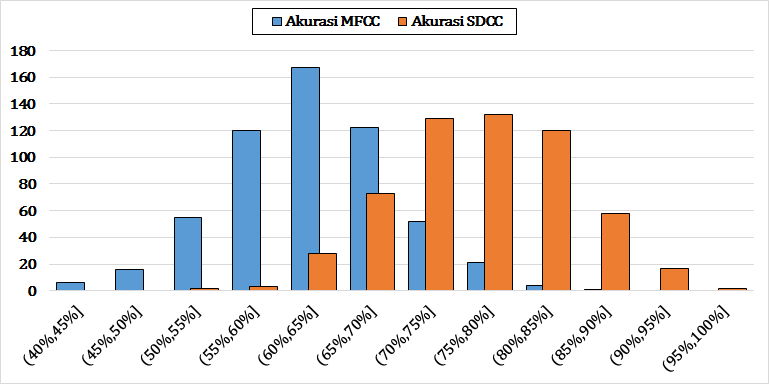
\includegraphics[width=\linewidth]{pics/histogram_akurasi_svm}
    \caption{Histogram Akurasi dengan Metode Klasifikasi SVM}
    \label{fig:histogramakurasisvm}
  \end{figure}

  Berdasarkan Gambar \ref{table:datahistogramakurasisvm}, penggunaan fitur SDCC mendominasi akurasi pada interval yang lebih tinggi jika dibandingkan dengan penggunaan fitur MFCC, dan perbedaannya terlihat secara signifikan.







  %-----------------------------------------------------------------------------%
  \subsection{Perbandingan Fitur pada Metode Klasifikasi GMM}
  %-----------------------------------------------------------------------------%
  Eksperimen yang menggunakan metode klasifikasi GMM dengan berbagai pengambilan fitur, memberikan hasil yang nilai akurasinya dirangkum pada Tabel \ref{table:perbandingangmm} berikut.

  \begin{table}
    \centering
    \caption{Perbandingan Hasil Eksperimen dengan Metode Klasifikasi GMM}
    \begin{tabular}{|c|c|c|}
      \hline
       & Akurasi MFCC & Akurasi SDCC \\ \hline
      Minimal         & 43.8\% & 67.5\% \\ \hline
      Maksimal        & 85.0\% & 98.8\% \\ \hline
      Rata-rata       & 65.8\% & 83.4\% \\ \hline
      Standar Deviasi & 0.065  & 0.056  \\ \hline
    \end{tabular}
    \label{table:perbandingangmm}
  \end{table}

  Tabel \ref{table:datahistogramakurasigmm} menunjukkan frekuensi kemunculan persentase tertentu yang dikelompokkan ke dalam interval 5\%.
  \begin{table}
    \centering
    \caption{Frekuensi Kemunculan Interval Persentase pada Eksperimen dengan Metode Klasifikasi GMM}
    \begin{tabular}{|c|c|c|}
      \hline
\multicolumn{1}{|c|}{Persentase} & \multicolumn{1}{c|}{\begin{tabular}[c]{@{}c@{}}Frekuensi Nilai\\ Akurasi MFCC\end{tabular}} & \multicolumn{1}{c|}{\begin{tabular}[c]{@{}c@{}}Frekuensi Nilai\\ Akurasi SDCC\end{tabular}} \\ \hline
(40\%,45\%{]}  & 2   & 0   \\ \hline
(45\%,50\%{]}  & 3   & 0   \\ \hline
(50\%,55\%{]}  & 27  & 0   \\ \hline
(55\%,60\%{]}  & 89  & 0   \\ \hline
(60\%,65\%{]}  & 144 & 0   \\ \hline
(65\%,70\%{]}  & 169 & 10  \\ \hline
(70\%,75\%{]}  & 94  & 36  \\ \hline
(75\%,80\%{]}  & 31  & 128 \\ \hline
(80\%,85\%{]}  & 5   & 193 \\ \hline
(85\%,90\%{]}  & 0   & 138 \\ \hline
(90\%,95\%{]}  & 0   & 53  \\ \hline
(95\%,100\%{]} & 0   & 6   \\ \hline
    \end{tabular}
    \label{table:datahistogramakurasigmm}
  \end{table}

  Gambar \ref{fig:histogramakurasigmm} merepresentasikan Tabel \ref{table:datahistogramakurasigmm} dalam bentuk histogram.
  \begin{figure}
    \centering
    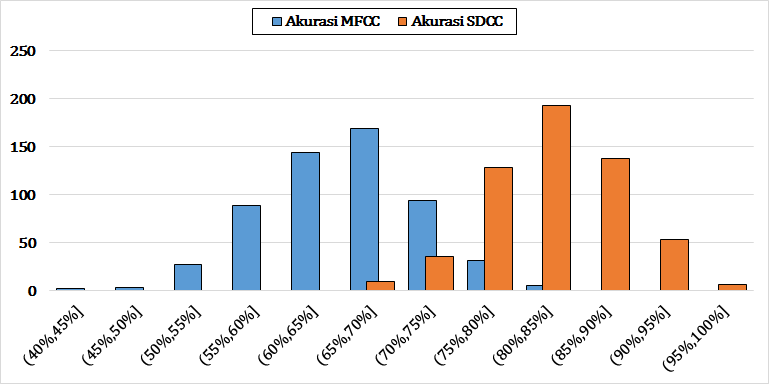
\includegraphics[width=\linewidth]{pics/histogram_akurasi_gmm}
    \caption{Histogram Akurasi dengan Metode Klasifikasi GMM}
    \label{fig:histogramakurasigmm}
  \end{figure}

  Berdasarkan Gambar \ref{table:datahistogramakurasigmm}, penggunaan fitur SDCC mendominasi akurasi pada interval yang lebih tinggi jika dibandingkan dengan penggunaan fitur MFCC, dan perbedaannya juga terlihat secara signifikan.





  
  %-----------------------------------------------------------------------------%
  \subsection{Perbandingan Fitur pada Metode Klasifikasi Gabungan}
  %-----------------------------------------------------------------------------%
  Eksperimen yang menggunakan metode klasifikasi gabungan antara SVM dan GMM dengan berbagai pengambilan fitur, memberikan hasil yang nilai akurasinya dirangkum pada Tabel \ref{table:perbandingangabungan} berikut.

  \begin{table}
    \centering
    \caption{Perbandingan Hasil Eksperimen dengan Metode Klasifikasi Gabungan}
    \begin{tabular}{|c|c|c|}
      \hline
       & Akurasi MFCC & Akurasi SDCC \\ \hline
      Minimal         & 41.3\% & 57.5\% \\ \hline
      Maksimal        & 85.0\% & 96.3\% \\ \hline
      Rata-rata       & 63.5\% & 79.4\% \\ \hline
      Standar Deviasi & 0.076  & 0.069  \\ \hline
    \end{tabular}
    \label{table:perbandingangabungan}
  \end{table}

  Tabel \ref{table:datahistogramakurasigabungan} menunjukkan frekuensi kemunculan persentase tertentu yang dikelompokkan ke dalam interval 5\%.
  \begin{table}
    \centering
    \caption{Frekuensi Kemunculan Interval Persentase pada Eksperimen dengan Metode Klasifikasi Gabungan}
    \begin{tabular}{|c|c|c|}
      \hline
\multicolumn{1}{|c|}{Persentase} & \multicolumn{1}{c|}{\begin{tabular}[c]{@{}c@{}}Frekuensi Nilai\\ Akurasi MFCC\end{tabular}} & \multicolumn{1}{c|}{\begin{tabular}[c]{@{}c@{}}Frekuensi Nilai\\ Akurasi SDCC\end{tabular}} \\ \hline
(40\%,45\%{]}  & 5   & 0   \\ \hline
(45\%,50\%{]}  & 19  & 0   \\ \hline
(50\%,55\%{]}  & 64  & 0   \\ \hline
(55\%,60\%{]}  & 115 & 2   \\ \hline
(60\%,65\%{]}  & 145 & 13  \\ \hline
(65\%,70\%{]}  & 104 & 49  \\ \hline
(70\%,75\%{]}  & 83  & 96  \\ \hline
(75\%,80\%{]}  & 24  & 161 \\ \hline
(80\%,85\%{]}  & 5   & 137 \\ \hline
(85\%,90\%{]}  & 0   & 83  \\ \hline
(90\%,95\%{]}  & 0   & 21  \\ \hline
(95\%,100\%{]} & 0   & 2   \\ \hline
    \end{tabular}
    \label{table:datahistogramakurasigabungan}
  \end{table}

  Gambar \ref{fig:histogramakurasigabungan} merepresentasikan Tabel \ref{table:datahistogramakurasigabungan} dalam bentuk histogram.
  \begin{figure}
    \centering
    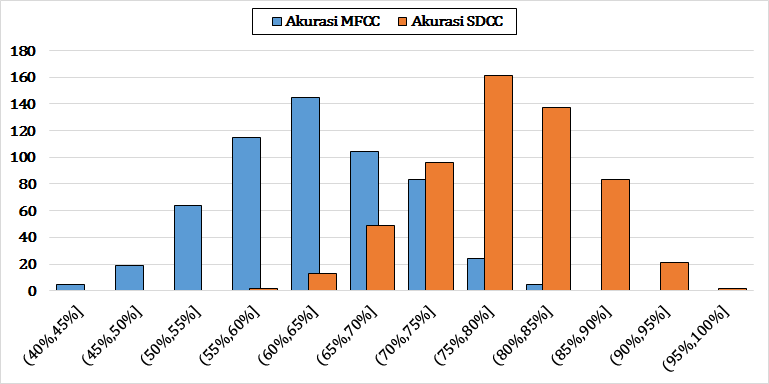
\includegraphics[width=\linewidth]{pics/histogram_akurasi_gabungan}
    \caption{Histogram Akurasi dengan Metode Klasifikasi Gabungan}
    \label{fig:histogramakurasigabungan}
  \end{figure}

  Berdasarkan Gambar \ref{table:datahistogramakurasigabungan}, penggunaan fitur SDCC mendominasi akurasi pada interval yang lebih tinggi jika dibandingkan dengan penggunaan fitur MFCC, dan perbedaannya terlihat secara signifikan. Hal itu semakin memperkuat pernyataan bahwa fitur SDCC lebih tepat untuk digunakan dalam sistem ini daripada fitur MFCC.














\section{Analisis Lanjut}

Penggunaan fitur SDCC dan metode klasifikasi GMM pada eksperimen memberikan hasil terbaik secara rata-rata, baik pada nilai akurasi, presisi, \f{recall}, ataupun \f{f-measure}. Setiap ayat memiliki hasil klasifikasi yang berbeda-beda. Ada ayat-ayat yang diklasifikasikan dengan akurasi tinggi dan ada juga ayat-ayat yang diklasifikasikan dengan akurasi rendah. Beberapa ayat dengan akurasi tertinggi yang lebih dari atau sama dengan 95\% pada penggunaan fitur SDCC dan metode klasifikasi GMM dapat dilihat pada Tabel \ref{table:akurasitinggi}.

\begin{table}
  \centering
  \caption{Ayat-Ayat yang Diurutkan dari Akurasi Tertinggi}
  \label{table:akurasitinggi}
  \begin{tabular}{|r|r|r|r|r|r|}
  \hline
  Surat & Ayat & Akurasi & Presisi & \f{Recall}  & \f{F-Measure} \\ \hline
  89  & 22 & 98.8\% & 97.6\%  & 100.0\% & 98.8\% \\ \hline
  91  & 13 & 97.5\% & 100.0\% & 95.0\%  & 97.4\% \\ \hline
  92  & 19 & 97.5\% & 97.5\%  & 97.5\%  & 97.5\% \\ \hline
  87  & 7  & 96.3\% & 95.1\%  & 97.5\%  & 96.3\% \\ \hline
  93  & 7  & 96.3\% & 97.4\%  & 95.0\%  & 96.2\% \\ \hline
  110 & 3  & 96.3\% & 100.0\% & 92.5\%  & 96.1\% \\ \hline
  78  & 19 & 95.0\% & 95.0\%  & 95.0\%  & 95.0\% \\ \hline
  79  & 31 & 95.0\% & 97.4\%  & 92.5\%  & 94.9\% \\ \hline
  79  & 46 & 95.0\% & 100.0\% & 90.0\%  & 94.7\% \\ \hline
  80  & 2  & 95.0\% & 100.0\% & 90.0\%  & 94.7\% \\ \hline
  80  & 25 & 95.0\% & 95.0\%  & 95.0\%  & 95.0\% \\ \hline
  88  & 21 & 95.0\% & 100.0\% & 90.0\%  & 94.7\% \\ \hline
  90  & 4  & 95.0\% & 100.0\% & 90.0\%  & 94.7\% \\ \hline
  \end{tabular}
\end{table}


Beberapa ayat dengan akurasi terendah yang kurang dari atau sama dengan 70\% pada penggunaan fitur SDCC dan metode klasifikasi GMM dapat dilihat pada Tabel \ref{table:akurasirendah}.
\begin{table}
  \centering
  \caption{Ayat-Ayat yang Diurutkan dari Akurasi Terendah}
  \label{table:akurasirendah}
  \begin{tabular}{|r|r|r|r|r|r|}
  \hline
  Surat & Ayat & Akurasi & Presisi & \f{Recall}  & \f{F-Measure} \\ \hline
  78    & 4    & 67.5\%  & 71.9\%  & 57.5\% & 63.9\%    \\ \hline
  83    & 4    & 67.5\%  & 64.6\%  & 77.5\% & 70.5\%    \\ \hline
  85    & 21   & 67.5\%  & 69.4\%  & 62.5\% & 65.8\%    \\ \hline
  101   & 10   & 67.5\%  & 71.9\%  & 57.5\% & 63.9\%    \\ \hline
  80    & 24   & 68.8\%  & 75.9\%  & 55.0\% & 63.8\%    \\ \hline
  106   & 1    & 68.8\%  & 75.9\%  & 55.0\% & 63.8\%    \\ \hline
  106   & 3    & 68.8\%  & 74.2\%  & 57.5\% & 64.8\%    \\ \hline
  106   & 4    & 68.8\%  & 71.4\%  & 62.5\% & 66.7\%    \\ \hline
  82    & 12   & 70.0\%  & 73.5\%  & 62.5\% & 67.6\%    \\ \hline
  85    & 6    & 70.0\%  & 76.7\%  & 57.5\% & 65.7\%    \\ \hline
  \end{tabular}
\end{table}

Suatu ayat dapat diklasifikasikan dengan akurasi tinggi dikarenakan ayat tersebut memiliki ciri khusus dalam pelafalannya jika dibandingkan dengan ayat-ayat lainnya. Ciri tersebut antara lain adalah bacaan \f{mad wajib} (bacaan panjang 3 huruf), \f{ghunnah} (bacaan dengung), serta irama panjang pendek dalam pembacaan ayat. Contoh beberapa ayat yang dapat diklasifikasikan dengan akurasi tinggi antara lain sebagai berikut.
\begin{itemize}
  \item Surat ke-89 ayat 22, yaitu ``\<وَجَاءَ رَبُّكَ وَالْمَلَكُ صَفًّا صَفًّا>''. Ayat tersebut mengandung \f{mad wajib} pada kata \<وَجَاءَ> serta \f{ghunnah} pada dua kata \<صَفًّا>.

  \item Surat ke-92 ayat 19, yaitu ``\<وَمَا لِأَحَدٍ عِندَهُ مِن نِّعْمَةٍ تُجْزَىٰ>''. Ayat tersebut mengandung \f{ghunnah} pada kata \<مِن نِّعْمَةٍ>.

  \item Surat ke-110 ayat 3, yaitu ``\<فَسَبِّحْ بِحَمْدِ رَبِّكَ وَاسْتَغْفِرْهُ ۚ إِنَّهُ كَانَ تَوَّابًا>''. Ayat tersebut mengandung \f{ghunnah} pada kata \<إِنَّهُ> dan \<تَوَّابًا>.
\end{itemize}


















% \section{Ayat-Ayat dengan Akurasi Tinggi}

% Berikut adalah beberapa tabel yang berisi ayat-ayat dengan nilai akurasi terbaik.

% \begin{enumerate}
%   \item Tabel \ref{table:topmfccsvm} menampilkan beberapa ayat yang diurutkan berdasarkan akurasi tertinggi pada eksperimen dengan fitur MFCC dan metode klasifikasi SVM.
%   \begin{table}
%     \centering
%     \caption{}
%     \label{table:topmfccsvm}
%     \begin{tabular}{|r|r|r|}
%       \hline
%       \textbf{Surat} & \textbf{Ayat} & \textbf{Akurasi} \\ \hline
%       99    & 7    & 87.5\%  \\ \hline
%       89    & 23   & 85.0\%  \\ \hline
%       91    & 14   & 82.5\%  \\ \hline
%       96    & 11   & 82.5\%  \\ \hline
%       79    & 16   & 81.3\%  \\ \hline
%       78    & 40   & 80.0\%  \\ \hline
%       79    & 45   & 80.0\%  \\ \hline
%       83    & 32   & 80.0\%  \\ \hline
%       84    & 10   & 80.0\%  \\ \hline
%       84    & 11   & 78.8\%  \\ \hline
%       99    & 8    & 78.8\%  \\ \hline
%       102   & 8    & 78.8\%  \\ \hline
%     \end{tabular}
%   \end{table}

%   \item Tabel \ref{table:topmfccgmm} menampilkan beberapa ayat yang diurutkan berdasarkan akurasi tertinggi pada eksperimen dengan fitur MFCC dan metode klasifikasi GMM.
%   \begin{table}
%     \centering
%     \caption{}
%     \label{table:topmfccgmm}
%     \begin{tabular}{|r|r|r|}
%       \hline
%       \textbf{Surat} & \textbf{Ayat} & \textbf{Akurasi} \\ \hline
%       89    & 1    & 85.0\%  \\ \hline
%       84    & 17   & 82.5\%  \\ \hline
%       79    & 45   & 81.3\%  \\ \hline
%       88    & 3    & 81.3\%  \\ \hline
%       106   & 2    & 81.3\%  \\ \hline
%       80    & 41   & 80.0\%  \\ \hline
%       83    & 32   & 80.0\%  \\ \hline
%       110   & 3    & 80.0\%  \\ \hline
%       79    & 46   & 78.8\%  \\ \hline
%       89    & 3    & 78.8\%  \\ \hline
%       89    & 18   & 78.8\%  \\ \hline
%       91    & 10   & 78.8\%  \\ \hline
%     \end{tabular}
%   \end{table}

%   \item Tabel \ref{table:topmfccgabungan} menampilkan beberapa ayat yang diurutkan berdasarkan akurasi tertinggi pada eksperimen dengan fitur MFCC dan metode klasifikasi gabungan.
%   \begin{table}
%     \centering
%     \caption{}
%     \label{table:topmfccgabungan}
%     \begin{tabular}{|r|r|r|}
%       \hline
%       \textbf{Surat} & \textbf{Ayat} & \textbf{Akurasi} \\ \hline
%       91 & 14 & 85.0\% \\ \hline
%       99 & 7  & 83.8\% \\ \hline
%       98 & 1  & 82.5\% \\ \hline
%       79 & 10 & 81.3\% \\ \hline
%       89 & 1  & 81.3\% \\ \hline
%       78 & 37 & 80.0\% \\ \hline
%       79 & 25 & 80.0\% \\ \hline
%       89 & 16 & 80.0\% \\ \hline
%       89 & 22 & 80.0\% \\ \hline
%       96 & 11 & 80.0\% \\ \hline
%     \end{tabular}
%   \end{table}

%   \item Tabel \ref{table:topsdccsvm} menampilkan beberapa ayat yang diurutkan berdasarkan akurasi tertinggi pada eksperimen dengan fitur SDCC dan metode klasifikasi SVM.
%   \begin{table}
%     \centering
%     \caption{}
%     \label{table:topsdccsvm}
%     \begin{tabular}{|r|r|r|}
%       \hline
%       \textbf{Surat} & \textbf{Ayat} & \textbf{Akurasi} \\ \hline
%       81  & 11 & 96.3\% \\ \hline
%       110 & 3  & 96.3\% \\ \hline
%       79  & 27 & 95.0\% \\ \hline
%       89  & 22 & 95.0\% \\ \hline
%       91  & 13 & 95.0\% \\ \hline
%       88  & 3  & 93.8\% \\ \hline
%       95  & 4  & 93.8\% \\ \hline
%       108 & 1  & 93.8\% \\ \hline
%       82  & 2  & 92.5\% \\ \hline
%       86  & 6  & 92.5\% \\ \hline
%       86  & 7  & 92.5\% \\ \hline
%       92  & 19 & 92.5\% \\ \hline
%     \end{tabular}
%   \end{table}

%   \item Tabel \ref{table:topsdccgmm} menampilkan beberapa ayat yang diurutkan berdasarkan akurasi tertinggi pada eksperimen dengan fitur SDCC dan metode klasifikasi GMM.
%   \begin{table}
%     \centering
%     \caption{}
%     \label{table:topsdccgmm}
%     \begin{tabular}{|r|r|r|}
%       \hline
%       \textbf{Surat} & \textbf{Ayat} & \textbf{Akurasi} \\ \hline
%       89  & 22 & 98.8\% \\ \hline
%       91  & 13 & 97.5\% \\ \hline
%       92  & 19 & 97.5\% \\ \hline
%       87  & 7  & 96.3\% \\ \hline
%       93  & 7  & 96.3\% \\ \hline
%       110 & 3  & 96.3\% \\ \hline
%       78  & 19 & 95.0\% \\ \hline
%       79  & 31 & 95.0\% \\ \hline
%       79  & 46 & 95.0\% \\ \hline
%       80  & 2  & 95.0\% \\ \hline
%       80  & 25 & 95.0\% \\ \hline
%       88  & 21 & 95.0\% \\ \hline
%       90  & 4  & 95.0\% \\ \hline
%     \end{tabular}
%   \end{table}

%   \item Tabel \ref{table:topsdccgabungan} menampilkan beberapa ayat yang diurutkan berdasarkan akurasi tertinggi pada eksperimen dengan fitur SDCC dan metode klasifikasi gabungan.
%   \begin{table}
%     \centering
%     \caption{}
%     \label{table:topsdccgabungan}
%     \begin{tabular}{|r|r|r|}
%       \hline
%       \textbf{Surat} & \textbf{Ayat} & \textbf{Akurasi} \\ \hline
%       78  & 19 & 96.3\% \\ \hline
%       110 & 3  & 96.3\% \\ \hline
%       78  & 36 & 95.0\% \\ \hline
%       78  & 39 & 95.0\% \\ \hline
%       79  & 31 & 95.0\% \\ \hline
%       93  & 7  & 95.0\% \\ \hline
%       85  & 12 & 93.8\% \\ \hline
%       89  & 18 & 93.8\% \\ \hline
%       89  & 22 & 93.8\% \\ \hline
%       78  & 14 & 92.5\% \\ \hline
%       80  & 25 & 92.5\% \\ \hline
%       87  & 5  & 92.5\% \\ \hline
%     \end{tabular}
%   \end{table}

% \end{enumerate}

% Dari Tabel {}, ..., diperoleh matriks kemunculan ayat pada tabel {} berikut.
% \begin{table}
%   \centering
%   \caption{}
%   \label{table:kemunculanayatpadatabel}
%   \begin{tabular}{|c|c|c|c|c|c|c|}
%     \hline
%     \textbf{Surat} & \textbf{Ayat} & \textbf{Akurasi} \\ \hline
%     78  & 19 & 96.3\% \\ \hline
%     110 & 3  & 96.3\% \\ \hline
%     78  & 36 & 95.0\% \\ \hline
%     78  & 39 & 95.0\% \\ \hline
%     79  & 31 & 95.0\% \\ \hline
%     93  & 7  & 95.0\% \\ \hline
%     85  & 12 & 93.8\% \\ \hline
%     89  & 18 & 93.8\% \\ \hline
%     89  & 22 & 93.8\% \\ \hline
%     78  & 14 & 92.5\% \\ \hline
%     80  & 25 & 92.5\% \\ \hline
%     87  & 5  & 92.5\% \\ \hline
%   \end{tabular}
% \end{table}

% \section{Ayat-Ayat dengan Akurasi Rendah}
%!TEX root = skripsi.tex
%-----------------------------------------------------------------------------%
\chapter{\babEnam}
%-----------------------------------------------------------------------------%

%-----------------------------------------------------------------------------%
\section{Kesimpulan}
%-----------------------------------------------------------------------------%
Setelah mengimplementasikan rancangan arsitektur sistem, menjalankan eksperimen, serta menganalisis hasil eksperimen, diperoleh kesimpulan sebagai berikut.

\begin{enumerate}
  \item Penggunaan fitur SDCC lebih baik daripada fitur MFCC. Hal ini dapat diamati dari nilai akurasi pada setiap metode klasifikasi pada Gambar \ref{fig:histogramakurasisvm}, Gambar \ref{fig:histogramakurasigmm}, dan Gambar \ref{fig:histogramakurasigabungan}. Histogram pada ketiga gambar tersebut menunjukkan hasil yang konsisten bahwa fitur SDCC lebih mendominasi akurasi di atas 70\% dibandingkan MFCC. Selain itu, nilai rata-rata akurasi antara fitur MFCC dengan fitur SDCC pada Tabel \ref{table:perbandingansvm}, Tabel \ref{table:perbandingangmm}, serta Tabel \ref{table:perbandingangabungan}, juga secara konsisten menunjukkan bahwa nilai rata-rata fitur SDCC lebih tinggi dari nilai rata-rata fitur MFCC pada berbagai metode klasifikasi. Perbedaan rata-rata akurasi antara fitur MFCC dengan fitur SDCC cukup signifikan, yaitu 14,2\% pada metode klasifikasi SVM, 17,6\% pada metode klasifikasi GMM, dan 15,9\% pada metode klasifikasi gabungan.

  \item Penggunaan metode klasifikasi GMM lebih baik daripada metode klasifikasi SVM maupun metode gabungan SVM dengan GMM. Hal ini dapat diamati dari nilai nilai rata-rata akurasi setiap metode klasifikasi pada Tabel \ref{table:perbandinganmfcc} dan Tabel \ref{table:perbandingansdcc}. Walaupun tidak signifikan, nilai rata-rata akurasi pada kedua tabel tersebut secara konsisten menunjukkan bahwa akurasi dengan metode klasifikasi GMM lebih tinggi daripada kedua metode klasifikasi yang lainnya. Histogram pada Gambar \ref{table:perbandinganmfcc} dan Gambar \ref{table:perbandingansdcc} juga menunjukkan bahwa metode klasifikasi GMM lebih mendominasi nilai-nilai akurasi yang lebih tinggi dari metode klasifikasi lainnya.

  \item Kombinasi pengambilan fitur SDCC dengan metode klasifikasi GMM adalah kombinasi yang memberikan hasil terbaik dalam penelitian ini. Hal ini dapat diamati dari nilai rata-rata akurasi pada Tabel \ref{table:mfccsvm}, Tabel \ref{table:mfccgmm}, Tabel \ref{table:mfccgabungan}, Tabel \ref{table:sdccsvm}, Tabel \ref{table:sdccgmm}, dan Tabel \ref{table:sdccgabungan}. Dari tabel-tabel tersebut kombinasi fitur SDCC dengan metode klasifikasi GMM menghasilkan nilai rata-rata akurasi tertinggi, yaitu sebesar 83,4\%.

  \item Penggabungan dua metode klasifikasi yang sama-sama memiliki kinerja yang baik tidak menjamin akan menghasilkan metode klasifikasi baru yang lebih baik lagi. Hal ini terlihat pada Tabel \ref{table:perbandinganmfcc} dan Tabel \ref{table:perbandingansdcc}. Nilai rata-rata akurasi dari metode klasifikasi GMM turun setelah digabung dengan metode klasifikasi SVM, baik pada pengambilan fitur MFCC maupun pada pengambilan fitur SDCC.

  \item Akurasi dari masing-masing ayat berbeda-beda. Ada beberapa ayat yang dapat diklasifikasikan dengan akurasi tinggi, dan ada juga beberapa ayat yang hanya diklasifikasikan dengan akurasi rendah.
\end{enumerate}

%-----------------------------------------------------------------------------%
\section{Saran}
%-----------------------------------------------------------------------------%
Setelah melakukan eksperimen, menganalisis hasil eksperimen, serta mengamati kesimpulan, ada beberapa saran untuk penelitian selanjutnya, antara lain sebagai berikut.

\begin{enumerate}
  \item Fitur MFCC dan fitur SDCC memungkinkan untuk dikombinasikan. Kombinasi ini layak untuk dicoba dalam penelitian selanjutnya karena ada peluang akurasi dari sistem akan akan meningkat.

  \item Sistem dalam penelitian ini dapat dikembangkan lebih lanjut supaya dapat memproses ayat-ayat \quran~yang panjang seperti di Surat Al-Baqarah, di mana terdapat ayat sepanjang satu halaman Al-Qur'an.

  \item Banyaknya data sampel dapat ditingkatkan, tidak hanya 40 sampel qari, untuk membangun sistem yang lebih \f{robust}.

  \item Banyak metode klasifikasi yang belum dicoba dalam penelitian ini. Ada kemungkinan metode klasifikasi lain menghasilkan akurasi yang lebih baik.

  \item Metode klasifikasi yang dilakukan dalam penelitian ini masih menggunakan parameter yang konstan. Ada potensi untuk meningkatkan akurasi sistem dengan memilih parameter yang lebih tepat pada setiap metode klasifikasi.
\end{enumerate}%!TEX root = skripsi.tex
%-----------------------------------------------------------------------------%
\begin{center}
\textbf{DAFTAR SINGKATAN}
\end{center}
%-----------------------------------------------------------------------------%%!TEX root = skripsi.tex
%
% Hyphenation untuk Indonesia 
%
% @author  Andreas Febrian
% @version 1.00
% 
% Tambahkan cara pemenggalan kata-kata yang salah dipenggal secara otomatis 
% oleh LaTeX. Jika kata tersebut dapat dipenggal dengan benar, maka tidak 
% perlu ditambahkan dalam berkas ini. Tanda pemenggalan kata menggunakan 
% tanda '-'; contoh:
% menarik
%   --> pemenggalan: me-na-rik
%

\hyphenation{
    % alphabhet A
    a-na-li-sa a-tur 
    a-pli-ka-si 
    % alphabhet B
    ba-ngun-an 
    be-be-ra-pa 
    ber-ge-rak
    ber-ke-lan-jut-an 
    ber-pe-nga-ruh 
    % alphabhet C
    ca-ri
    % alphabhet D
    di-ban-ding-kan
    di-de-fi-ni-si-kan
    di-ha-rap-kan
    di-ka-te-go-ri-kan
    di-mi-li-ki-nya
    di-se-rah-kan
    di-sim-pan di-pim-pin de-ngan da-e-rah di-ba-ngun da-pat di-nya-ta-kan 
    di-sim-bol-kan di-pi-lih di-li-hat de-fi-ni-si
    di-se-su-ai-kan
    % alphabhet E
    e-le-men
    e-ner-gi eks-klu-sif
    % alphabhet F
    fa-si-li-tas
    % alphabhet G
    ga-bung-an ge-rak
    % alphabhet H
    ha-lang-an
    he-te-ro-gen
    % alphabhet I
    i-ngin
    % alphabhet J
    % alphabhet K
    ke-hi-lang-an
    ku-ning 
    kua-li-tas ka-me-ra ke-mung-kin-an ke-se-pa-ham-an
    ke-te-pat-an
    kon-fi-gu-ra-si
    % alphabhet L
    ling-kung-an
    % alphabhet M
    me-min-ta
    me-mo-del-kan
    me-mo-ri
    men-de-fi-ni-si-kan
    me-neng-ah
    meng-a-tas-i me-mung-kin-kan me-nge-na-i me-ngi-rim-kan 
    meng-u-bah meng-a-dap-ta-si me-nya-ta-kan mo-di-fi-ka-si
    meng-a-tur
    meng-au-to-ma-si
    meng-a-ko-mo-da-si
    me-ngo-rek-si
    % alphabhet N
    nya-ta non-eks-klu-sif
    % alphabhet O
    % alphabhet P
    pa-ra-lel
    peng-ala-mat-an
    pen-ting
    penga-da-an
		pe-nye-rap-an 
		pe-ngon-trol
    pe-mo-del-an
    pe-ran  pe-ran-an-nya
    pe-rin-tah
    pem-ba-ngun-an pre-si-den pe-me-rin-tah prio-ri-tas peng-am-bil-an 
    peng-ga-bung-an pe-nga-was-an pe-ngem-bang-an 
    pe-nga-ruh pa-ra-lel-is-me per-hi-tung-an per-ma-sa-lah-an 
    pen-ca-ri-an peng-struk-tur-an
    pe-ner-bang-an
    pro-se-sor
    % alphabhet Q
    % alphabhet R
    ran-cang-an
    % alphabhet S
    se-dang-kan
    se-ring
    si-mu-la-si sa-ngat    
    % alphabhet T
    te-ngah
    ter-da-pat
    % alphabhet U
    u-sa-ha
    % alphabhet V
    % alphabhet W
    % alphabhet X
    % alphabhet Y
    % alphabhet Z
    % special
    MATLAB
    basmalah
    sam-ping
    hardware
    software
    mem-ba-ca
    teks-tual
    automatically
}%!TEX root = skripsi.tex
%
% @author  Andreas Febrian
% @version 1.00
% 
% Mendaftar seluruh istilah yang mungkin akan perlu dijadikan 
% italic atau bold pada setiap kemunculannya dalam dokumen. 
% 

\var{\license}{\f{Creative Common License 1.0 Generic}}
\var{\bslash}{$\setminus$}
\var{\ioa}{\f{input}}
\var{\iob}{\f{output}}
\var{\br}{\f{bit rate}}
\var{\fr}{\f{frame}}
\var{\quran}{Al-Qur'an}%!TEX root = skripsi.tex
%
% Halaman Judul Laporan 
%
% @author  unknown
% @version 1.01
% @edit by Andreas Febrian
%

\begin{titlepage}
    \begin{center}\begin{figure}
            \begin{center}
                
\includegraphics[width=2.5cm]{pics/makara.png}
            \end{center}
        \end{figure}    
        \vspace*{0cm}
        \bo{
        	UNIVERSITAS INDONESIA\\
        }
        
        \vspace*{1.0cm}
        % judul thesis harus dalam 14pt Times New Roman
        \bo{\Judul} \\[1.0cm]

        \vspace*{2.5 cm}    
        % harus dalam 14pt Times New Roman
        \bo{\Type} \\
        % keterangan prasyarat
        \bo{Diajukan sebagai salah satu syarat untuk memperoleh gelar \\
        \gelar}\\

        \vspace*{3 cm}       
        % penulis dan npm
        \bo{\Penulis} \\
        \bo{\npm} \\

        \vspace*{5.0cm}

        % informasi mengenai fakultas dan program studi
        \bo{
        	FAKULTAS \Fakultas\\
        	PROGRAM STUDI \Program \\
        	DEPOK \\
        	\bulanTahun
        }
    \end{center}
\end{titlepage}%!TEX root = skripsi.tex
%!TEX root = skripsi.tex
%-----------------------------------------------------------------------------%
% Informasi Mengenai Dokumen
%-----------------------------------------------------------------------------%
% 
% Judul laporan. 
\var{\judul}{Evaluasi Pembacaan Al-Qur'an Otomatis menggunakan Sistem Pengenalan Suara}
% 
% Tulis kembali judul laporan, kali ini akan diubah menjadi huruf kapital
\Var{\Judul}{Evaluasi Pembacaan Al-Qur'an Otomatis menggunakan Sistem Pengenalan Suara}
% 
% Tulis kembali judul laporan namun dengan bahasa Ingris
\var{\judulInggris}{Automatic Quran Recitation Evaluation using Speech Recognition System}

% 
% Tipe laporan, dapat berisi Skripsi, Tugas Akhir, Thesis, atau Disertasi
\var{\type}{Skripsi}
% 
% Tulis kembali tipe laporan, kali ini akan diubah menjadi huruf kapital
\Var{\Type}{Skripsi}
% 
% Tulis nama penulis 
\var{\penulis}{Alfan Nur Fauzan}
% 
% Tulis kembali nama penulis, kali ini akan diubah menjadi huruf kapital
\Var{\Penulis}{Alfan Nur Fauzan}
% 
% Tulis NPM penulis
\var{\npm}{1206219086}
% 
% Tuliskan Fakultas dimana penulis berada
\Var{\Fakultas}{Ilmu Komputer}
\var{\fakultas}{Ilmu Komputer}
% 
% Tuliskan Program Studi yang diambil penulis
\Var{\Program}{Ilmu Komputer}
\var{\program}{Ilmu Komputer}
\var{\programEng}{Computer Science}
% 
% Tuliskan tahun publikasi laporan
\Var{\bulanTahun}{Juni 2015}
% 
% Tuliskan gelar yang akan diperoleh dengan menyerahkan laporan ini
\var{\gelar}{Sarjana Ilmu Komputer}
% 
% Tuliskan tanggal pengesahan laporan, waktu dimana laporan diserahkan ke 
% penguji/sekretariat
\var{\tanggalPengesahan}{20 Juni 2015} 
% 
% Tuliskan tanggal keputusan sidang dikeluarkan dan penulis dinyatakan 
% lulus/tidak lulus
\var{\tanggalLulus}{20 Juni 2015}
% 
% Tuliskan pembimbing 
\var{\pembimbing}{Dra. Mirna Adriani, Ph.D.}
\var{\pembimbingdua}{Dr. Amalia Zahra}
% 
% Alias untuk memudahkan alur penulisan paa saat menulis laporan
\var{\saya}{penulis}
\var{\Saya}{Penulis}

%-----------------------------------------------------------------------------%
% Judul Setiap Bab
%-----------------------------------------------------------------------------%
% 
% Berikut ada judul-judul setiap bab. 
% Silahkan diubah sesuai dengan kebutuhan. 
% 
\Var{\kataPengantar}{Kata Pengantar}
\Var{\babSatu}{Pendahuluan}
\Var{\babDua}{Landasan Teori}
\Var{\babTiga}{Perancangan Sistem}
\Var{\babEmpat}{Eksperimen}
\Var{\babLima}{Hasil Eksperimen dan Analisis}
\Var{\babEnam}{Kesimpulan dan Saran}
%!TEX root = skripsi.tex
%
% @author  Andreas Febrian
% @version 1.00 
% 
% Hanya sebuah pembatas bertuliskan LAMPIRAN ditengah halaman. 
% 

\begin{titlepage}
	\centering 
	\vspace*{6cm}
	\noindent \Huge{LAMPIRAN}
	\addChapter{LAMPIRAN}
\end{titlepage}%!TEX root = skripsi.tex
%
% Halaman Orisinalitas
%
% @author  Andreas Febrian
% @version 1.01
%

\chapter*{\uppercase{halaman pernyataan orisinalitas}}
\vspace*{2cm}

\begin{center}
	\bo{\type~ini adalah hasil karya saya sendiri, \\ 
	dan semua sumber baik yang dikutip maupun dirujuk \\
	telah saya nyatakan dengan benar.} \\
	\vspace*{2.6cm}
	
	\begin{tabular}{l c l}
	\bo{Nama} & : & \bo{\penulis} \\
	\bo{NPM} & : & \bo{\npm} \\ 
	\bo{Tanda Tangan} & : & \\
	& & \\
	& & \\
	\bo{Tanggal} & : & \bo{\tanggalPengesahan} \\	
	\end{tabular}
\end{center}

\newpage%!TEX root = skripsi.tex
%-----------------------------------------------------------------------------%
\chapter*{\kataPengantar}
%-----------------------------------------------------------------------------%

\begin{arabtex}الْحَمْدُ لِلَّـهِ الَّذِي هَدَانَا لِهَـٰذَا وَمَا كُنَّا لِنَهْتَدِيَ لَوْلَا أَنْ هَدَانَا اللَّـهُ\end{arabtex} \f{Segala puji bagi Allah yang telah menunjuki kami kepada (surga) ini. Dan kami sekali-kali tidak akan mendapat petunjuk kalau Allah tidak memberi kami petunjuk. [Al-A'raf:43]}\begin{arabtex}الْحَمْدُ للهِ رَبِّ الْعَالَمِيْنَ، وَالصَّلاَةُ وَالسَّلاَمُ عَلَى سَيِّدِنَا مُحَمَّدٍ سَيِّدِ اْلأَوَّلِيْنَ وَالآخِرِيْنَ، وَعَلَى آلِهِ وَصَحْبِهِ وَمَنِ اهْتَدَى بِهَدْيِهِ إِلَى يَوْمِ الدَّيْنِ\end{arabtex} \f{Segala puji bagi Allah, Tuhan sekalian alam, semoga keselamatan dan kesejahteraan tetap terlimpahkan atas junjungan kita Nabi Muhammad SAW, penghulu manusia, baik yang dahulu maupun yang belakangan, begitu juga kepada segenap keluarga dan semua orang yang mengikuti petunjuk, sampai saat Hari Kemudian.} Segala puji dan syukur kehadirat Allah SWT, Tuhan Yang Maha Esa, yang senantiasa memberikan ramhat dan hidayah-Nya, sehingga \saya~dapat menyelesaikan skripsi ini.

Penulisan skripsi ini ditujukan untuk memenuhi salah satu syarat untuk menyelesaikan pendidikan pada Program \gelar, Universitas Indonesia. \Saya~sadar bahwa dalam perjalanan menuntut ilmu di universitas hingga dalam menyelesaikan skripsi ini, \saya~tidak sendiri. \Saya~ingin berterima kasih kepada pihak-pihak yang selalu peduli, mendampingi, dan mendukung \saya, yaitu:

\begin{enumerate}
	\item Kedua Orang Tua \saya~yang selalu memberikan dukungan dan do'a kepada \saya.
	\item Dra. Mirna Adriani, Ph.D. dan Dr. Amalia Zahra selaku dosen pembimbing yang banyak memberikan arahan, masukan, dan bantuan dalam menyelesaikan skripsi ini.
  \item Alfan Farizki Wicaksono, ST., M.Sc. dan Rahmad Mahendra, S.Kom., M.Sc. yang memberi dukungan dari awal sampai akhir pengerjaan skripsi ini, dan juga memberikan tips-tips dalam mengerjakan skripsi.
  \item Andreas Febrian yang telah membuat \f{template} dokumen skripsi ini, sehingga \saya~menjadi terbantu dalam menulis skripsi.
  \item Erik Dominikus yang telah mempublikasikan dan mempopulerkan \f{template} dokumen skripsi ini, sehingga \saya~menjadi tahu bahwa ada \f{template} tersebut.
	\item Mohammad Syahid Wildan dan Abid Nurul Hakim, sebagai rekan yang banyak memberi masukan dan berbagi ide dengan \saya.
  \item Teman-teman Lab Information Retrieval yang memberi dukungan dan semangat kepada \saya~untuk menyelesaikan skripsi ini.
  \item Teman-teman Forum Remaja Masjid UI yang memberi dukungan serta do'a kepada \saya~untuk menyelesaikan skripsi ini.
	\item Pihak-pihak lain yang tidak dapat \saya~sebutkan satu-persatu yang sudah memberikan bantuan dan dukungannya kepada \saya.
\end{enumerate}
\vspace*{0.1cm}
\begin{flushright}
Depok, Juni 2016\\[0.1cm]
\vspace*{1cm}
\penulis

\end{flushright}%!TEX root = skripsi.tex
%
% Halaman Pengesahan Sidang
%
% @author  Andreas Febrian, Andre Tampubolon 
% @version 1.02
%

\chapter*{HALAMAN PENGESAHAN}

\vspace*{0.4cm}
\noindent 

\noindent
\begin{tabular}{ll p{9cm}}
	\type~ini diajukan oleh&: & \\
	Nama&: & \penulis \\
	NPM&: & \npm \\
	Program Studi&: & \program \\
	Judul \type&: & \judul \\
\end{tabular} \\

\vspace*{1.0cm}

\noindent \bo{Telah berhasil dipertahankan di hadapan Dewan Penguji 
dan diterima sebagai bagian persyaratan yang diperlukan untuk 
memperoleh gelar \gelar~pada Program Studi \program, Fakultas 
\fakultas, Universitas Indonesia.}\\[0.2cm]

\begin{center}
	\bo{DEWAN PENGUJI}
\end{center}

\vspace*{0.3cm}

\begin{tabular}{l l l l }
	& & & \\
	Pembimbing&: & \pembimbing & (\hspace*{3.0cm}) \\
	& & & \\
	Penguji&: &  & (\hspace*{3.0cm}) \\
	& & & \\
	Penguji&: &  & (\hspace*{3.0cm}) \\
\end{tabular}\\

\vspace*{2.0cm}

\begin{tabular}{ll l}
	Ditetapkan di&: & Depok\\
	Tanggal&: & \tanggalLulus \\
\end{tabular}


\newpage%!TEX root = skripsi.tex
%
% Halaman Pengesahan
%
% @author  Andreas Febrian
% @author  Ardhi Putra Pratama
% @version 1.1
%

\chapter*{HALAMAN PERSETUJUAN}

\vspace*{0.2cm}
\noindent 

\noindent
\begin{tabular}{l l p{11cm}}
	\bo{Judul}&: & \judul \\ 
	\bo{Nama}&: & \penulis \\
	\bo{NPM}&: & \npm \\
\end{tabular} \\

\vspace*{1.2cm}


\noindent\begin{minipage}[b]{0.6\hsize}
  \raggedright
  Laporan \type~ini telah diperiksa dan disetujui.\\[0.3cm]
  
  \tanggalPengesahan \\[2cm]
  
  \underline{\pembimbing}\\[0.1cm]
  Pembimbing \type
\end{minipage}
\hfill
\begin{minipage}[b]{0.4\hsize}
  \raggedleft
  .\\[2cm]
  \underline{\pembimbingdua}\\[0.1cm]
  Pembimbing \type
\end{minipage}

\newpage%!TEX root = skripsi.tex
% 
% @author  Andre Tampubolon, Andreas Febrian
% @version 1.01
% 

\chapter*{\uppercase{Halaman Pernyataan Persetujuan Publikasi Tugas Akhir untuk Kepentingan Akademis}}

\vspace*{0.2cm}
\noindent 
Sebagai sivitas akademik Universitas Indonesia, saya yang bertanda 
tangan di bawah ini:
\vspace*{0.4cm}


\begin{tabular}{p{4.2cm} l p{6cm}}
	\bo{Nama} & : & \penulis \\ 	
	\bo{NPM} & : & \npm \\
	\bo{Program Studi} & : & \program\\	
	\bo{Fakultas} & : & \fakultas\\
	\bo{Jenis Karya} & : & \type \\
\end{tabular}

\vspace*{0.6cm}
\noindent demi pengembangan ilmu pengetahuan, menyetujui untuk memberikan 
kepada Universitas Indonesia \bo{Hak Bebas Royalti Noneksklusif 
(Non-exclusive Royalty Free Right)} atas karya ilmiah saya yang berjudul:
\begin{center}
	\judul
\end{center}
beserta perangkat yang ada (jika diperlukan). Dengan Hak Bebas Royalti 
Noneksklusif ini Universitas Indonesia berhak menyimpan, 
mengalihmedia/formatkan, mengelola dalam bentuk pangkalan data 
(\f{database}), merawat, dan memublikasikan tugas akhir saya selama 
tetap mencantumkan nama saya sebagai penulis/pencipta dan sebagai 
pemilik Hak Cipta. \\

\noindent Demikian pernyatan ini saya buat dengan sebenarnya.

\begin{center}
	\vspace*{0.8cm}
	\begin{tabular}{lll}
		Dibuat di&: & Depok \\
		Pada tanggal&: & \tanggalPengesahan \\
	\end{tabular}\\

	\vspace*{0.2cm}
	Yang menyatakan \\
	\vspace*{2cm}
	(\penulis)
\end{center}

\newpage

%!TEX root = skripsi.tex
%
% Sampul Laporan

%
% @author  unknown
% @version 1.01
% @edit by Andreas Febrian
%

\begin{titlepage}
    \begin{center}    
        \begin{figure}
            \begin{center}
                
\includegraphics[width=2.5cm]{pics/makara.png}
            \end{center}
        \end{figure}    
        \vspace*{0cm}
        \bo{
        	UNIVERSITAS INDONESIA\\
        }
        
        \vspace*{1.0cm}
        % judul thesis harus dalam 14pt Times New Roman
        \bo{\Judul} \\[1.0cm]

        \vspace*{2.5 cm}    
        % harus dalam 14pt Times New Roman
        \bo{\Type}

        \vspace*{3 cm}       
        % penulis dan npm
        \bo{\Penulis} \\
        \bo{\npm} \\

        \vspace*{5.0cm}

        % informasi mengenai fakultas dan program studi
        \bo{
        	FAKULTAS \Fakultas\\
        	PROGRAM STUDI \Program \\
        	DEPOK \\
        	\bulanTahun
        }
    \end{center}
\end{titlepage}
%!TEX root = skripsi.tex
%
% Template Laporan Skripsi/Thesis 
%
% @author  Andreas Febrian, Lia Sadita 
% @version 1.03
%
% Dokumen ini dibuat berdasarkan standar IEEE dalam membuat class untuk 
% LaTeX dan konfigurasi LaTeX yang digunakan Fahrurrozi Rahman ketika 
% membuat laporan skripsi. Konfigurasi yang lama telah disesuaikan dengan 
% aturan penulisan thesis yang dikeluarkan UI pada tahun 2008.
%

%
% Tipe dokumen adalah report dengan satu kolom. 
%
\documentclass[12pt, a4paper, onecolumn, oneside, final]{report}

\usepackage{arabtex}
\usepackage{utf8}
\setcode{utf8}
\usepackage{amsmath}
\usepackage{amssymb}
\usepackage{enumitem}

\usepackage{natbib}
% Load konfigurasi LaTeX untuk tipe laporan thesis
\usepackage{uithesis}


\newcolumntype{L}[1]{>{\raggedright\let\newline\\\arraybackslash\hspace{0pt}}m{#1}}
\newcolumntype{C}[1]{>{\centering\let\newline\\\arraybackslash\hspace{0pt}}m{#1}}
\newcolumntype{R}[1]{>{\raggedleft\let\newline\\\arraybackslash\hspace{0pt}}m{#1}}
% Load konfigurasi khusus untuk laporan yang sedang dibuat
%!TEX root = skripsi.tex
%-----------------------------------------------------------------------------%
% Informasi Mengenai Dokumen
%-----------------------------------------------------------------------------%
% 
% Judul laporan. 
\var{\judul}{Pengenalan Entitas Kesehatan pada Forum Online dengan Menggunakan Recurrent Neural Networks}
% 
% Tulis kembali judul laporan, kali ini akan diubah menjadi huruf kapital
\Var{\Judul}{Pengenalan Entitas Kesehatan pada Forum Online dengan Menggunakan Recurrent Neural Networks}
% 
% Tulis kembali judul laporan namun dengan bahasa Ingris
\var{\judulInggris}{Medical Entity Recognition on the Online Health Forum using Recurrent Neural Networks}

% 
% Tipe laporan, dapat berisi Skripsi, Tugas Akhir, Thesis, atau Disertasi
\var{\type}{Skripsi}
% 
% Tulis kembali tipe laporan, kali ini akan diubah menjadi huruf kapital
\Var{\Type}{Skripsi}
% 
% Tulis nama penulis 
\var{\penulis}{Wahid Nur Rohman}
% 
% Tulis kembali nama penulis, kali ini akan diubah menjadi huruf kapital
\Var{\Penulis}{Wahid Nur Rohman}
% 
% Tulis NPM penulis
\var{\npm}{1306381856}
% 
% Tuliskan Fakultas dimana penulis berada
\Var{\Fakultas}{Ilmu Komputer}
\var{\fakultas}{Ilmu Komputer}
% 
% Tuliskan Program Studi yang diambil penulis
\Var{\Program}{Ilmu Komputer}
\var{\program}{Ilmu Komputer}
\var{\programEng}{Computer Science}
% 
% Tuliskan tahun publikasi laporan
\Var{\bulanTahun}{Juli 2016}
% 
% Tuliskan gelar yang akan diperoleh dengan menyerahkan laporan ini
\var{\gelar}{Sarjana Ilmu Komputer}
% 
% Tuliskan tanggal pengesahan laporan, waktu dimana laporan diserahkan ke 
% penguji/sekretariat
\var{\tanggalPengesahan}{22 Juli 2016}
% 
% Tuliskan tanggal keputusan sidang dikeluarkan dan penulis dinyatakan 
% lulus/tidak lulus
\var{\tanggalLulus}{27 Juni 2016}
% 
% Tuliskan pembimbing 
\var{\pembimbing}{Dra. Mirna Adriani, Ph.D.}
\var{\pembimbingdua}{Alfan Farizki Wicaksono S.T., M.Sc.}
% 
% Alias untuk memudahkan alur penulisan paa saat menulis laporan
\var{\saya}{penulis}
\var{\Saya}{Penulis}

%-----------------------------------------------------------------------------%
% Judul Setiap Bab
%-----------------------------------------------------------------------------%
% 
% Berikut ada judul-judul setiap bab. 
% Silahkan diubah sesuai dengan kebutuhan. 
% 
\Var{\kataPengantar}{Kata Pengantar}
\Var{\babSatu}{Pendahuluan}
\Var{\babDua}{Landasan Teori}
\Var{\babTiga}{Metodologi}
\Var{\babEmpat}{Eksperimen}
\Var{\babLima}{Hasil Eksperimen dan Analisis}
\Var{\babEnam}{Kesimpulan dan Saran}

% Daftar pemenggalan suku kata dan istilah dalam LaTeX
%!TEX root = skripsi.tex
%
% Hyphenation untuk Indonesia 
%
% @author  Andreas Febrian
% @version 1.00
% 
% Tambahkan cara pemenggalan kata-kata yang salah dipenggal secara otomatis 
% oleh LaTeX. Jika kata tersebut dapat dipenggal dengan benar, maka tidak 
% perlu ditambahkan dalam berkas ini. Tanda pemenggalan kata menggunakan 
% tanda '-'; contoh:
% menarik
%   --> pemenggalan: me-na-rik
%

\hyphenation{
    % alphabhet A
    a-na-li-sa a-tur 
    a-pli-ka-si 
    % alphabhet B
    ba-ngun-an 
    be-be-ra-pa 
    ber-ge-rak
    ber-ke-lan-jut-an 
    ber-pe-nga-ruh 
    % alphabhet C
    ca-ri
    % alphabhet D
    di-ban-ding-kan
    di-de-fi-ni-si-kan
    di-ha-rap-kan
    di-ka-te-go-ri-kan
    di-mi-li-ki-nya
    di-se-rah-kan
    di-sim-pan di-pim-pin de-ngan da-e-rah di-ba-ngun da-pat di-nya-ta-kan 
    di-sim-bol-kan di-pi-lih di-li-hat de-fi-ni-si
    di-se-su-ai-kan
    % alphabhet E
    e-le-men
    e-ner-gi eks-klu-sif
    % alphabhet F
    fa-si-li-tas
    % alphabhet G
    ga-bung-an ge-rak
    % alphabhet H
    ha-lang-an
    he-te-ro-gen
    % alphabhet I
    i-ngin
    % alphabhet J
    % alphabhet K
    ke-hi-lang-an
    ku-ning 
    kua-li-tas ka-me-ra ke-mung-kin-an ke-se-pa-ham-an
    ke-te-pat-an
    kon-fi-gu-ra-si
    % alphabhet L
    ling-kung-an
    % alphabhet M
    me-min-ta
    me-mo-del-kan
    me-mo-ri
    men-de-fi-ni-si-kan
    me-neng-ah
    meng-a-tas-i me-mung-kin-kan me-nge-na-i me-ngi-rim-kan 
    meng-u-bah meng-a-dap-ta-si me-nya-ta-kan mo-di-fi-ka-si
    meng-a-tur
    meng-au-to-ma-si
    meng-a-ko-mo-da-si
    me-ngo-rek-si
    % alphabhet N
    nya-ta non-eks-klu-sif
    % alphabhet O
    % alphabhet P
    pa-ra-lel
    peng-ala-mat-an
    pen-ting
    penga-da-an
		pe-nye-rap-an 
		pe-ngon-trol
    pe-mo-del-an
    pe-ran  pe-ran-an-nya
    pe-rin-tah
    pem-ba-ngun-an pre-si-den pe-me-rin-tah prio-ri-tas peng-am-bil-an 
    peng-ga-bung-an pe-nga-was-an pe-ngem-bang-an 
    pe-nga-ruh pa-ra-lel-is-me per-hi-tung-an per-ma-sa-lah-an 
    pen-ca-ri-an peng-struk-tur-an
    pe-ner-bang-an
    pro-se-sor
    % alphabhet Q
    % alphabhet R
    ran-cang-an
    % alphabhet S
    se-dang-kan
    se-ring
    si-mu-la-si sa-ngat    
    % alphabhet T
    te-ngah
    ter-da-pat
    % alphabhet U
    u-sa-ha
    % alphabhet V
    % alphabhet W
    % alphabhet X
    % alphabhet Y
    % alphabhet Z
    % special
    MATLAB
    basmalah
    sam-ping
    hardware
    software
    voiced
    overlap
    frame
    bit
    rate
    support
    vector
    machine
    Gaussian
    mixture
    model
    dynamic
    pro-gram-ming
    auto-ma-tically
    mem-ba-ca
    teks-tual
    eks-trak-si
    di-je-las-kan
    be-nar
    sa-lah
    teks-tual
    dengan
    me-re-pre-sen-ta-si
    me-re-pre-sen-ta-si-kan
}
% Daftar istilah yang mungkin perlu ditandai 
%!TEX root = skripsi.tex
%
% @author  Andreas Febrian
% @version 1.00
% 
% Mendaftar seluruh istilah yang mungkin akan perlu dijadikan 
% italic atau bold pada setiap kemunculannya dalam dokumen. 
% 

\var{\license}{\f{Creative Common License 1.0 Generic}}
\var{\bslash}{$\setminus$}
\var{\ioa}{\f{input}}
\var{\iob}{\f{output}}
\var{\br}{\f{bit rate}}
\var{\fr}{\f{frame}}
\var{\quran}{Al-Qur'an}
\var{\mer}{MER}
\var{\rnn}{\f{Recurrent Neural Networks}}
\var{\ol}{\f{online}}
\var{\disease}{\f{disease}}
\var{\symptom}{\f{symptom}}
\var{\drug}{\f{drug}}
\var{\treatment}{\f{treatment}}
\var{\Disease}{\f{Disease}}
\var{\Symptom}{\f{Symptom}}
\var{\Drug}{\f{Drug}}
\var{\Treatment}{\f{Treatment}}
\var{\we}{\f{word embedding}}
\var{\radit}{Raditya Herwando}
\var{\skripsiRadit}{\cite{skripsiKakRadit}}

%\usepackage[backend=bibtex]{biblatex}
%\addbibresource{bib.bib}

% Awal bagian penulisan laporan
\begin{document}
%
% Sampul Laporan
%!TEX root = skripsi.tex
%
% Sampul Laporan

%
% @author  unknown
% @version 1.01
% @edit by Andreas Febrian
%

\begin{titlepage}
    \begin{center}    
        \begin{figure}
            \begin{center}
                
\includegraphics[width=2.5cm]{pics/makara.png}
            \end{center}
        \end{figure}    
        \vspace*{0cm}
        \bo{
        	UNIVERSITAS INDONESIA\\
        }
        
        \vspace*{1.0cm}
        % judul thesis harus dalam 14pt Times New Roman
        \bo{\Judul} \\[1.0cm]

        \vspace*{2.5 cm}    
        % harus dalam 14pt Times New Roman
        \bo{\Type}

        \vspace*{3 cm}       
        % penulis dan npm
        \bo{\Penulis} \\
        \bo{\npm} \\

        \vspace*{5.0cm}

        % informasi mengenai fakultas dan program studi
        \bo{
        	FAKULTAS \Fakultas\\
        	PROGRAM STUDI \Program \\
        	DEPOK \\
        	\bulanTahun
        }
    \end{center}
\end{titlepage}


%
% Gunakan penomeran romawi
\pagenumbering{roman}

%
% load halaman judul dalam
\addChapter{HALAMAN JUDUL}
%!TEX root = skripsi.tex
%
% Halaman Judul Laporan 
%
% @author  unknown
% @version 1.01
% @edit by Andreas Febrian
%

\begin{titlepage}
    \begin{center}\begin{figure}
            \begin{center}
                
\includegraphics[width=2.5cm]{pics/makara.png}
            \end{center}
        \end{figure}    
        \vspace*{0cm}
        \bo{
        	UNIVERSITAS INDONESIA\\
        }
        
        \vspace*{1.0cm}
        % judul thesis harus dalam 14pt Times New Roman
        \bo{SEMANTIC ROLE LABELING UNTUK BAHASA INDONESIA PERCAKAPAN DENGAN MENGGUNAKAN DEEP LEARNING} \\[1.0cm]

        \vspace*{2.5 cm}    
        % harus dalam 14pt Times New Roman
        \bo{\Type} \\
        % keterangan prasyarat
        \bo{Diajukan sebagai salah satu syarat untuk memperoleh gelar \\
        \gelar}\\

        \vspace*{3 cm}       
        % penulis dan npm
        \bo{\Penulis} \\
        \bo{\npm} \\

        \vspace*{5.0cm}

        % informasi mengenai fakultas dan program studi
        \bo{
        	FAKULTAS \Fakultas\\
        	PROGRAM STUDI \Program \\
        	DEPOK \\
        	\bulanTahun
        }
    \end{center}
\end{titlepage}

%
% setelah bagian ini, halaman dihitung sebagai halaman ke 2
\setcounter{page}{2}

% sementara ga usah
% load halaman pengesahan
%\addChapter{LEMBAR PERSETUJUAN}
%\documentclass[12pt, a4paper, onecolumn, oneside, final]{report}
\usepackage{pdfpages}
\begin{document}
\includepdf[pages=4]{../skripsi}
\end{document}
%
% load halaman orisinalitas 
\addChapter{LEMBAR PERNYATAAN ORISINALITAS}
%!TEX root = skripsi.tex
%
% Halaman Orisinalitas
%
% @author  Andreas Febrian
% @version 1.01
%

\chapter*{\uppercase{halaman pernyataan orisinalitas}}
\vspace*{2cm}

\begin{center}
	\bo{\type~ini adalah hasil karya saya sendiri, \\ 
	dan semua sumber baik yang dikutip maupun dirujuk \\
	telah saya nyatakan dengan benar.} \\
	\vspace*{2.6cm}
	
	\begin{tabular}{l c l}
	\bo{Nama} & : & \bo{\penulis} \\
	\bo{NPM} & : & \bo{\npm} \\ 
	\bo{Tanda Tangan} & : & \\
	& & \\
	& & \\
	\bo{Tanggal} & : & \bo{\tanggalPengesahan} \\	
	\end{tabular}
\end{center}

\newpage
%
%
\addChapter{LEMBAR PENGESAHAN}
%!TEX root = skripsi.tex
%
% Halaman Pengesahan Sidang
%
% @author  Andreas Febrian, Andre Tampubolon 
% @version 1.02
%

\chapter*{HALAMAN PENGESAHAN}

\vspace*{0.4cm}
\noindent 

\noindent
\begin{tabular}{ll p{9cm}}
	\type~ini diajukan oleh&: & \\
	Nama&: & \penulis \\
	NPM&: & \npm \\
	Program Studi&: & \program \\
	Judul \type&: & \judul \\
\end{tabular} \\

\vspace*{1.0cm}

\noindent \bo{Telah berhasil dipertahankan di hadapan Dewan Penguji 
dan diterima sebagai bagian persyaratan yang diperlukan untuk 
memperoleh gelar \gelar~pada Program Studi \program, Fakultas 
\fakultas, Universitas Indonesia.}\\[0.2cm]

\begin{center}
	\bo{DEWAN PENGUJI}
\end{center}

\vspace*{0.3cm}

\begin{tabular}{l l l l }
	& & & \\
	Pembimbing 1&: & \pembimbing & (\hspace*{3.0cm}) \\
	& & & \\
	Pembimbing 2&: & \pembimbingdua & (\hspace*{3.0cm}) \\
	& & & \\
	Penguji&: & - & (\hspace*{3.0cm}) \\
	& & & \\
	Penguji&: & - & (\hspace*{3.0cm}) \\
\end{tabular}\\

\vspace*{2.0cm}

\begin{tabular}{ll l}
	Ditetapkan di&: & Depok\\
	Tanggal&: & \tanggalLulus \\
\end{tabular}


\newpage
%
%
\addChapter{\kataPengantar}
%!TEX root = skripsi.tex
%-----------------------------------------------------------------------------%
\chapter*{\kataPengantar}
%-----------------------------------------------------------------------------%

Segala puji bagi Allah, Tuhan semesta alam, semoga keselamatan dan kesejahteraan tetap terlimpahkan atas junjungan kita Nabi Muhammad SAW, sebaik-baik teladan bagi umat manusia. Segala puji dan syukur kehadirat Allah SWT, Tuhan Yang Maha Esa, yang telah memberikan pertolongan, sehingga \saya~dapat menyelesaikan skripsi ini.

Penulisan skripsi ini ditujukan untuk memenuhi salah satu syarat untuk menyelesaikan pendidikan pada Program \gelar, Universitas Indonesia. \Saya~sadar bahwa dalam perjalanan menuntut ilmu di universitas hingga dalam menyelesaikan skripsi ini, \saya~tidak sendiri. \Saya~ingin berterima kasih kepada pihak-pihak yang selalu peduli, mendampingi, dan mendukung \saya, yaitu:

\begin{enumerate}
	\item Kedua Orang Tua \saya~yang selalu memberikan dukungan dan do'a kepada \saya.
	\item Dra. Mirna Adriani, Ph.D. dan Alfan Farizki Wicaksono S.T., M.Sc. selaku dosen pembimbing yang banyak memberikan arahan, masukan, dan bantuan dalam menyelesaikan skripsi ini.
  \item Rahmad Mahendra, S.Kom., M.Sc. yang telah memberikan banyak masukan dan saran dalam menyelesaikan skripsi ini.
  \item Andreas Febrian yang telah membuat \f{template} dokumen skripsi ini, sehingga \saya~menjadi terbantu dalam menulis skripsi.
  \item Erik Dominikus yang telah mempublikasikan dan mempopulerkan \f{template} dokumen skripsi ini, sehingga \saya~menjadi tahu bahwa ada \f{template} tersebut.
  \item Alfan Nur Fauzan yang telah memberikan \f{template} dokumen skripsi yang telah diperbaiki ini, sehingga saya sangat terbantu dalam melakukan penulisan
	\item Putu Wira Astika Dharma, Andi Fajar Nur Ismail dan Ken Nabila Setya, sebagai rekan yang banyak memberi masukan dan berbagi ide dengan \saya.
  \item Teman-teman Lab Information Retrieval yang memberi dukungan dan semangat kepada \saya~untuk menyelesaikan skripsi ini.
  \item Segenap teman-teman angkatan 2013 (Angklung) yang memberi dukungan dan semangat kepada \saya~untuk menyelesaikan skripsi ini.
	\item Pihak-pihak lain yang tidak dapat \saya~sebutkan satu-persatu yang sudah memberikan bantuan dan dukungannya kepada \saya.
\end{enumerate}
\vspace*{0.1cm}
\begin{flushright}
Depok, Desember 2017\\[0.1cm]
\vspace*{1cm}
\penulis

\end{flushright}
%
%
\addChapter{LEMBAR PERSETUJUAN PUBLIKASI ILMIAH}
%!TEX root = skripsi.tex
% 
% @author  Andre Tampubolon, Andreas Febrian
% @version 1.01
% 

\chapter*{\uppercase{Halaman Pernyataan Persetujuan Publikasi Tugas Akhir untuk Kepentingan Akademis}}

\vspace*{0.2cm}
\noindent 
Sebagai sivitas akademik Universitas Indonesia, saya yang bertanda 
tangan di bawah ini:
\vspace*{0.4cm}


\begin{tabular}{p{4.2cm} l p{6cm}}
	\bo{Nama} & : & \penulis \\ 	
	\bo{NPM} & : & \npm \\
	\bo{Program Studi} & : & \program\\	
	\bo{Fakultas} & : & \fakultas\\
	\bo{Jenis Karya} & : & \type \\
\end{tabular}

\vspace*{0.6cm}
\noindent demi pengembangan ilmu pengetahuan, menyetujui untuk memberikan 
kepada Universitas Indonesia \bo{Hak Bebas Royalti Noneksklusif 
(Non-exclusive Royalty Free Right)} atas karya ilmiah saya yang berjudul:
\begin{center}
	\judul
\end{center}
beserta perangkat yang ada (jika diperlukan). Dengan Hak Bebas Royalti 
Noneksklusif ini Universitas Indonesia berhak menyimpan, 
mengalihmedia/formatkan, mengelola dalam bentuk pangkalan data 
(\f{database}), merawat, dan memublikasikan tugas akhir saya selama 
tetap mencantumkan nama saya sebagai penulis/pencipta dan sebagai 
pemilik Hak Cipta. \\

\noindent Demikian pernyatan ini saya buat dengan sebenarnya.

\begin{center}
	\vspace*{0.8cm}
	\begin{tabular}{lll}
		Dibuat di&: & Depok \\
		Pada tanggal&: & \tanggalPengesahan \\
	\end{tabular}\\

	\vspace*{0.2cm}
	Yang menyatakan \\
	\vspace*{2cm}
	(\penulis)
\end{center}

\newpage


%
% 
\singlespacing
\addChapter{ABSTRAK}
%!TEX root = skripsi.tex
%
% Halaman Abstrak
%
% @author  Andreas Febrian
% @version 1.00
%

\chapter*{Abstrak}

\vspace*{0.2cm}

\noindent \begin{tabular}{l l p{10cm}}
	Nama&: & \penulis \\
	Program Studi&: & \program \\
	Judul&: & Semantic Role Labeling untuk Bahasa Indonesia Percakapan dengan Menggunakan Deep Learning \\
\end{tabular} \\ 

\vspace*{0.5cm}

\noindent 

\textit{Semantic Role Labeling} (SRL) telah diteliti cukup dalam, terutama untuk Bahasa Inggris yang formal. Akan tetapi, hanya terdapat sedikit riset untuk bahasa percakapan informal, terutama untuk bahasa yang digunakan dalam sistem \textit{chatbot}. Dalam Bahasa Indonesia, kedua jenis bahasa formal dan percakapan masih sedikit diteliti untuk membangun sistem SRL. Pada riset ini, kami berfokus pada menyelesaikan permasalahan SRL untuk Bahasa Indonesia percakapan. Kontribusi kami adalah memperkenalkan set \textit{semantic roles} baru dan mengajukan \textit{attention mechanism} di atas arsitektur \textit{Long Short-Term Memory Networks}. Tantangan dalam Bahasa Indonesia percakapan adalah \textit{slang} dan singkatan, kalimat pendek, dan struktur yang tidak beraturan. Walaupun riset ini merupakan \textit{pilot task}, kami memperoleh hasil yang menjanjikan dengan nilai F1 82.68\%.


\vspace*{0.2cm}

\noindent Keywords: \\ 
\noindent Semantic Role Labeling, deep learning, bahasa percakapan, RNNs \\ 

\newpage
%
%
%!TEX root = skripsi.tex
%
% Halaman Abstract
%
% @author  Andreas Febrian
% @version 1.00
%

\chapter*{ABSTRACT}

\vspace*{0.2cm}

\noindent \begin{tabular}{l l p{11.0cm}}
	Name&: & \penulis \\
	Program&: & \programEng \\
	Title&: & \judulInggris \\
\end{tabular} \\ 

\vspace*{0.5cm}

\noindent 

Nowadays, everyone can use online health forums for seeking information regarding health issues without directly visiting a doctor in the hospital. There are thousands of health-related posts generated by thousands of online users everyday. As a result, A huge amount of information can be extracted from such online forums. In this work, we focus on seeking a good computational model to automatically extract the names of disease, symptom, treatment, and drug due to its usefulness for future task, such as Medical Question Answering systems. Furthermore, we formulate our problem as a sequence labeling problem using machine learning approach. We propose Deep Learning technique using Recurrent Neural Networks (RNNs), because RNNs is state-of-the-art for sequence labeling problem. We propose some features such as word features, medical dictionary, stop word, POS-Tag, word phrase(verb and noun), word before and word after. Furthermore we propose two RNNs architectures, which are LSTMs in one layer and LSTMs in two layer with multi-input. The result of this experiment shows that the model proposed can give the good result. Based on the experiment using the combination features of its own word, medical dictionary, stop word, word phrase (noun and verb), 1 word before and 1 word after using the first RNNs architecture achieve f-measure $ 63.06\% $, and using second RNNs architecture achieve f-measure $ 62.14\% $. Thats result is better than the baseline used \citep{skripsiKakRadit}, f-measure $ 54.09\% $.


\vspace*{0.2cm}

\noindent Keywords: \\ 
\noindent \mer, RNNs, disease, symptom, treatment, drug \\ 

\newpage

%
% Daftar isi, gambar, dan tabel
%
\tableofcontents
\clearpage
\listoffigures
\clearpage
\listoftables
\clearpage
% \lstlistoflistings
% \clearpage

%
% Gunakan penomeran Arab (1, 2, 3, ...) setelah bagian ini.
%
\pagenumbering{arabic}

%
%
%
\onehalfspacing
%!TEX root = skripsi.tex
%-----------------------------------------------------------------------------%
\chapter{\babSatu}
%-----------------------------------------------------------------------------%


%-----------------------------------------------------------------------------%
\section{Latar Belakang}
%-----------------------------------------------------------------------------%
	
	Saat ini, perkembangan teknologi semakin mempermudah berbagai kegiatan manusia yang dilakukan sehari-hari. Sebagai contoh, ketika seseorang mengalami permasalahan kesehatan dan ingin berkonsultasi kepada para dokter, ia dapat memanfaatkan forum kesehatan \textit{online} yang dapat memungkinkan terjadinya interaksi antara pasien dan dokter tanpa perlu tatap muka.  Melalui forum tersebut, seseorang hanya perlu menuliskan keluhan dan pertanyaan pada formulir yang tersedia. Kemudian, dokter yang memiliki akun di forum kesehatan \textit{online} tersebut dapat memberikan jawaban atas pertanyaan orang tersebut.
	
	Banyak sekali informasi bermanfaat yang dapat diperoleh dari forum kesehatan \textit{online}. Informasi tersebut meliputi informasi keluhan yang dialami pasien, obat yang sebaiknya digunakan atau langkah penyembuhan yang dapat dilakukan. Orang lain dapat mencari obat atau langkah penyembuhan dari forum tersebut melalui pertanyaan yang sudah diajukan sebelumnya. Oleh karena itu, akan sangat baik apabila ada sebuah model atau sistem yang mampu mengekstrak secara otomatis informasi-informasi tersebut. Tantangan utama dari pengembangan model ini adalah \textit{post} atau isi dari forum yang tidak terstruktur. Dokumen \textit{post} tidak dibagi menjadi beberapa bagian seperti bagian keluhan, penyakit, obat dan lain sebagainya, namun hanya menjadi satu bagian saja. Misalnya ketika seseorang menanyakan tentang keluhannya, orang tersebut hanya diberikan dua buah isian berupa judul dan isi pertanyaan. Jawaban yang diberikan oleh dokter juga sama, hanya menjadi satu bagian saja. Jawaban yang diberikan tidak terstruktur seperti memiliki bagian langkah penyembuhan, nama penyakit dan obat secara terpisah. Hal ini menyebabkan orang sulit melakukan ekstraksi informasi dari dokumen tersebut.
	
	Dari permasalahan tersebut, terdapat sebuah solusi untuk melakukan ekstraksi informasi penyakit dalam suatu dokumen, yaitu dengan menggunakan sistem Pengenalan Entitas Kesehatan (\textit{Medical Entity Recognition}) atau disingkat MER. Sistem \mer~ini dapat mengenali entitas kesehatan dalam sebuah dokumen. Apabila diberikan sebuah dokumen, sistem ini akan mengembalikan dokumen yang telah mendapatkan label pada masing-masing entitas kesehatan di dalamnya.
	
	Penelitian dalam rangka mengembangkan sistem \mer~sudah banyak dilakukan oleh beberapa peneliti. Salah satu penelitian tersebut dilakukan oleh \cite{abacha2011medical} dengan menggunakan dokumen medis rumah sakit berbahasa Inggris. Entitas yang mendapatkan label pada penelitian tersebut adalah \textit{treatment}, \textit{problem} dan \textit{test}. Terdapat tiga pendekatan yang digunakan, yaitu pendekatan \textit{machine learning}, pendekatan \textit{rule based} dan pendekatan \textit{hybrid}. Kesimpulan yang dicapai pada penelitian tersebut adalah pendekatan \textit{hybrid} memberikan hasil terbaik, yaitu dengan \textit{precision} $ 72.18\% $, \textit{recall} $ 83.78\% $ dan \textit{F-Measure} $ 77.55\% $.
		
	Pada dokumen berbahasa Indonesia, pengembangan sistem \mer~masih belum banyak dilakukan. Ada beberapa penelitian terkait sistem \mer, namun hasil yang diberikan belum memuaskan. Salah satu penelitian terkait \mer~dilakukan oleh \cite{skripsiKakRadit} yang menggunakan dokumen forum kesehatan \textit{online} berbahasa Indonesia dari beberapa situs. Tujuan dari penelitian tersebut adalah untuk mencari kombinasi fitur yang dapat menghasilkan akurasi terbaik. \cite{skripsiKakRadit} menggunakan algoritma \textit{Conditional Random Fields} dengan hasil akhir yaitu \textit{precission}~70.97\%, \textit{recall}~57.83\% dan \textit{f-measure}~63.69\%. Fitur-fitur yang membuat model memiliki akurasi terbaik yaitu fitur kata itu sendiri, frasa, kamus (\textit{symptom, disease, treatment, drug}), \textit{window feature (previous word)} dan panjang kata.
	
	Dalam penelitian ini \saya~memandang permasalahan pelabelan dokumen kesehatan sebagai permasalahan \textit{sequence labeling}. \Saya~mengusulkan penggunaan teknik \textit{Deep Learning} dengan menggunakan \textit{Recurrent Neural Networks} (RNNs), karena RNNs merupakan \textit{state-of-the-art} untuk permasalahan \textit{sequence labeling} seperti permasalahan pada penelitian ini. Sebelumnya penelitian terkait hal ini pernah dikerjakan oleh \cite{mujiono2016new}, dengan jenis entitas yang digunakan adalah entitas \textit{Drug} saja. Peneliti tersebut menggunakan model RNNs untuk melabeli dokumen secara otomatis. Dengan menggunakan fitur vektor kata yang menggunakan \textit{word embedding} saja, \textit{f-measure} yang diberikan mencapai 86.45\%. Oleh karena itu, \saya~mengusulkan model RNNs pada penelitian ini.
		
	\Saya~berharap bahwa penelitian ini akan memberikan banyak manfaat. Sistem \mer~yang dihasilkan dapat digunakan untuk membuat aplikasi lain. Misalnya dengan adanya \mer~pada dokumen bahasa Indonesia, dapat dibuat sistem untuk melakukan \textit{indexing} dokumen forum sehingga pencarian dokumen kesehatan dapat dilakukan dengan lebih efisien. Selain itu, keluaran dari \mer~juga dapat digunakan untuk mengidentifikasi tren penyakit pada waktu tertentu dari suatu sumber, sehingga pihak terkait mampu melakukan langkah dan kebijakan yang tepat. Sistem \mer~juga dapat digunakan pada aplikasi \textit{Question Answering} \citep{abacha2011medical} dengan cara memanfaatkan hasil pelabelan untuk melakukan identifikasi entitas yang ditanyakan. Gambar \ref{fig:merforqa} merupakan contoh penggunaan \mer~pada aplikasi \textit{question answering} dalam bidang kesehatan.
	
	\begin{figure}
		\centering
		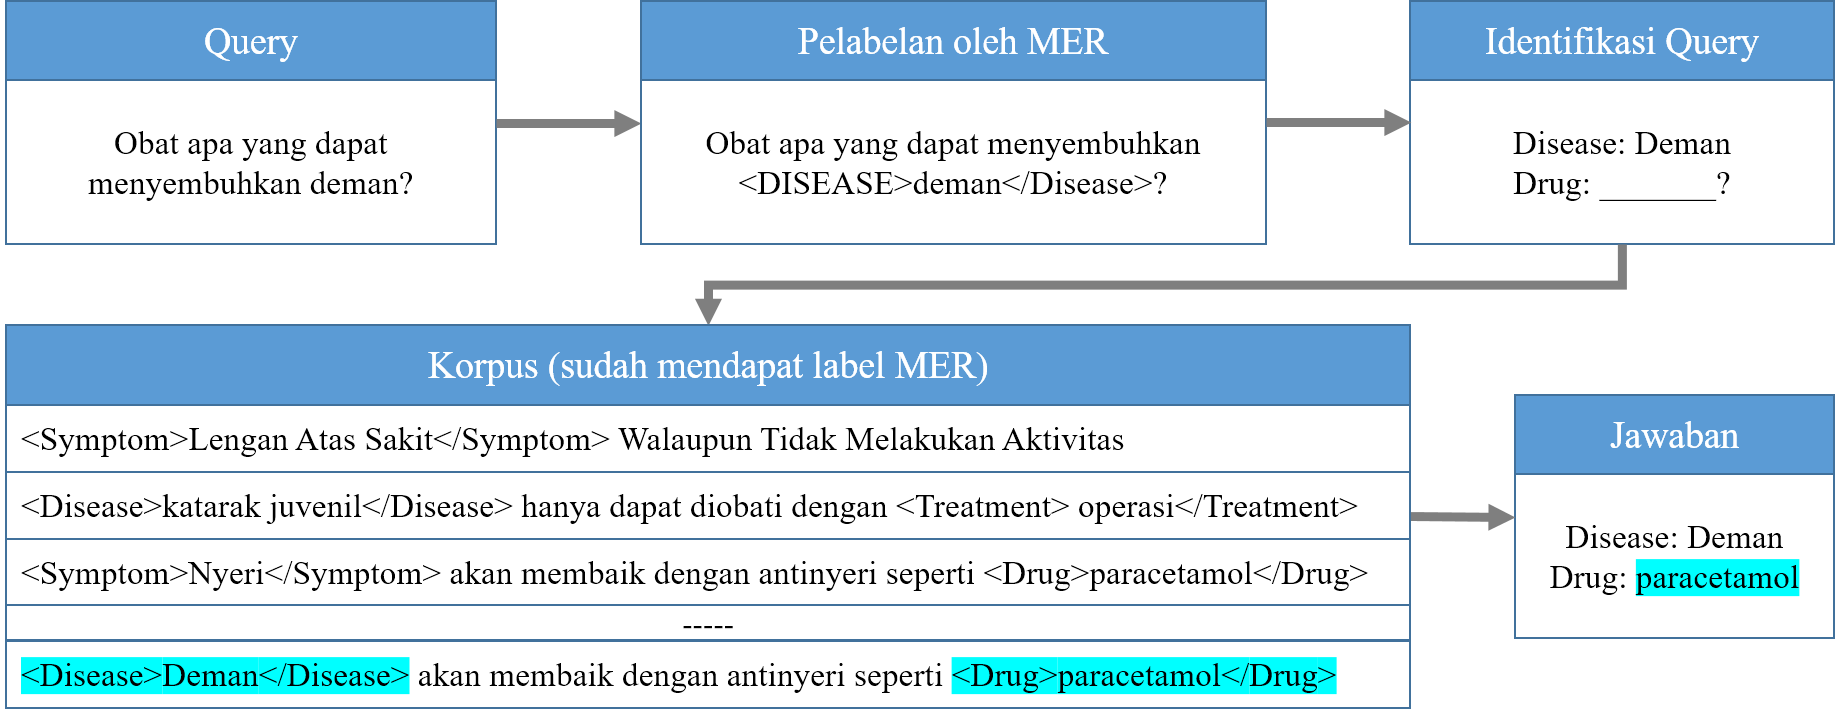
\includegraphics[width=\linewidth]{images/merforqa}
		\caption{Diagram Penggunaan MER pada aplikasi \textit{Question Answering}}
		\label{fig:merforqa}
	\end{figure}
	
	\Saya~berharap bahwa penelitian \mer~pada dokumen berbahasa Indonesia ini dapat dilanjutkan sehingga dapat menghasilkan model yang lebih baik dan membuat suatu aplikasi yang memanfaatkan keluaran dari penelitian ini. Masih banyak manfaat lain yang didapatkan dengan adanya sistem \mer~yang memiliki hasil akurat. 

%-----------------------------------------------------------------------------%
\section{Perumusan Masalah}
%-----------------------------------------------------------------------------%
Berdasarkan latar belakang di atas, dalam penelitian ini \saya~ mengajukan rumusan masalah sebagai berikut:
\begin{enumerate}
	% Bagaimana --- %
	\item Bagaimana performa RNNs dibandingkan dengan CRFs (\textit{baseline}) untuk sistem \mer~yang dikembangkan?
	\item Fitur apa saya yang membuat sistem \mer~memiliki performa terbaik?
\end{enumerate}

%-----------------------------------------------------------------------------%
\section{Tujuan dan Manfaat Penelitian}
%-----------------------------------------------------------------------------%
Penelitian ini bertujuan untuk membangun sistem yang mampu melakukan ekstraksi entitas kesehatan dari forum \textit{online}. Sebenarnya, pada penelitan yang dilakukan oleh \cite{skripsiKakRadit} sudah menghasilkan sebuah sistem yang sama. Namun, fokus penelitian ini yaitu mencoba menggunakan metode yang berbeda. Metode tersebut yaitu dengan menggunakan RNNs dengan harapan mampu memberikan hasil yang lebih baik. Penelitian ini juga bertujuan untuk mendapatkan fitur-fitur yang membuat sistem memiliki performa terbaik. Selain itu, penelitian ini juga bertujuan untuk mendapatkan informasi baru terkait pembuatan sistem \mer~berbahasa Indonesia.

Manfaat dari penelitian ini adalah menghasilkan rancangan sistem dan metode yang dapat digunakan sebagai bahan penelitian lanjutan. Saat ini, sistem dan metode yang dihasilkan hanya mampu mengenali entitas kesehatan saja. Hal ini dapat digunakan untuk membuat sistem informasi tentang suatu jenis penyakit lengkap dengan gejala, obat dan cara penyembuhannya. Selama ini, masyarakat yang menanyakan suatu penyakit melalui forum \ol~tidak membaca terlebih dahulu riwayat pertanyaan yang telah ditanyakan oleh orang lain. Oleh karena itu, diharapkan dengan sistem informasi tersebut, calon penanya hanya perlu mencari penyakit yang akan ditanyakan pada sistem informasi tersebut. Apabila tidak ada, penanya dapat mengajukan pertanyaan, kemudian pertanyaan dan jawaban yang diberikan akan terindeks oleh sistem dan menambah informasi. 

Selain itu, hasil penelitian ini juga dapat digunakan untuk membangun sistem yang mengenali tren penyakit pada masyarakat, sehingga pihak terkait mampu menentukan langkah strategis yang tepat. Sistem \mer~juga dapat digunakan pada aplikasi \textit{Question Answering} \citep{abacha2011medical} dengan cara memanfaatkan hasil pelabelan untuk melakukan identifikasi entitas yang ditanyakan.

%-----------------------------------------------------------------------------%
\section{Metodologi Penelitian}
%-----------------------------------------------------------------------------%
Berikut merupakan metode penelitian yang \saya~lakukan.
\begin{enumerate}
	\item Studi Literatur\\
	Pada tahapan ini \saya~mencari literatur yang terkait dengan penelitian ini. Literatur ini digunakan sebagai bahan pemelajaran dan untuk mendukung penelitian yang \saya~lakukan. Literatur yang \saya~gunakan memiliki keterkaitan terhadap kasus \mer, \textit{Sequence Labeling} dan \rnn.
	
	\item Pengumpulan Data \\
	Pada tahapan ini, \saya~mengumpulkan data percobaan yang diperlukan. \Saya~mengumpulkan dokumen teks dari forum kesehatan \textit{online} dan dari penelitian \cite{skripsiKakRadit}. Setelah dokumen terkumpul, \saya~melakukan langkah-langkah pra-pemrosesan baik pada dokumen yang \saya~dapatkan dari forum maupun korpus dari penelitian \cite{skripsiKakRadit}. Tujuan langkah tersebut yaitu untuk menghilangkan beberapa karakter yang mengganggu tahapan selanjutnya, melakukan normalisasi pada beberapa kasus token, dan lain sebagainya. Setelah itu \saya~melakukan tokenisasi dan melakukan pemecahan kalimat dengan menggunakan beberapa aturan, kemudian \saya~memberikan label pada dokumen yang \saya~dapat dari forum secara manual. 
	
	\item Pengembangan Model\\
	Pada tahapan ini, \saya~melakukan perancangan eksperimen yang akan dilakukan. \Saya~mendefinisikan fitur-fitur yang akan diuji pada penelitian ini dan arsitektur RNNs yang juga akan diuji.
		
	\item Eksperimen \\
	Tahapan ini merupakan bagian inti dari penelitian. \saya~melakukan langkah eksperimen dengan tujuan mendapatkan jawaban dari pertanyaan yang telah dirumuskan pada rumusan masalah. Sebelum masuk di tahap ini, \saya~melakukan pemecahan data menjadi 10 bagian untuk mengimplementasikan \textit{10-cross fold validation}. Setelah itu, data disusun sedemikian sehingga siap digunakan sebagai \textit{resource} eksperimen.
	
	\item Evaluasi dan Analisis Hasil \\
	Pada tahapan ini \saya~melakukan evaluasi dan analisis dari hasil eksperimen. Untuk mengukur akurasi dari masing-masing fitur dan arsitektur RNNs yang \saya~usulkan, saya menggunakan \textit{precision}, \textit{recall} dan \textit{f-measure}.
		
	\item Penarikan Kesimpulan \\
	Tahap ini merupakan tahap terakhir dari penelitian. Setelah melakukan serangkaian eksperimen, evaluasi dan analisis, \saya~memberikan kesimpulan dan informasi penting terkait penelitian ini. Selain itu \saya~juga memberikan saran untuk penelitian selanjutnya.
\end{enumerate}

%-----------------------------------------------------------------------------%
\section{Ruang Lingkup Penelitian}
Pada penelitian ini terdapat beberapa batasan yang \saya~tentukan, yaitu:
\begin{enumerate}
\item{\bf Entitas Kesehatan}\\
Pengenalan entitas kesehatan pada penelitian ini berfokus pada pengenalan nama penyakit (\disease), gejala-gejala penyakit (\symptom), nama obat (\drug) dan langkah pengobatan (\treatment),

\item{\bf Domain Pengenalan}\\
Pengenalan entitas kesehatan dilakukan pada bagian judul pertanyaan, isi pertanyaan/keluhan dan isi jawaban dari dokter.
\end{enumerate}

%-----------------------------------------------------------------------------%

%-----------------------------------------------------------------------------%
\section{Sistematika Penulisan}
%-----------------------------------------------------------------------------%
Sistematika penulisan dalam laporan penelitian ini sebagai berikut:
\begin{itemize}

	\item Bab 1 \babSatu \\
	Pada bab ini \saya~menjelaskan mengenai motivasi dalam melakukan penelitian ini dan komponen-komponen utama penelitian seperi latar belakang, perumusan masalah, tujuan dan manfaat penelitian, metodologi penelitian, ruang lingkup penelitian dan sistematika penulisan.
	
	\item Bab 2 \babDua \\
	Pada bab ini \saya~melakukan studi literatur mengenai beberapa teori dan penelitian yang dilakukan oleh penulis lain. 
		
	\item Bab 3 \babTiga \\
	Pada bab ini \saya~menjelaskan alur dari penelitian ini, yaitu pengumpulan data, pra-pemrosesan, pelabelan, pengembangan model, eksperimen dan evaluasi.
		
	\item Bab 4 \babEmpat \\
	Pada bab ini \saya~menjelaskan proses implementasi sistem dan eksperimen berdasarkan rancangan yang telah \penulis~tentukan pada bab sebelumnya. Selain itu \saya~juga menjelaskan implementasi dari masing-masing tahapan yang dilakukan.
		
	\item Bab 5 \babLima \\
	Pada bab ini \saya~menjelaskan analisis dari hasil eksperimen yang telah \saya~kerjakan pada tahap sebelumnya. Hasil eksperimen \saya~sajikan dalam bentuk tabel dan grafik.
	
	\item Bab 6 \babEnam \\
	Pada bab ini \saya~memberikan kesimpulan berdasarkan hasil eksperimen dan analisis yang telah dilakukan pada penelitian ini. Selain itu \saya~juga memberikan saran dan masukan untuk penelitian dan pengembangan sistem mengenai \mer~berbahasa Indonesia selanjutnya.
	
\end{itemize}
%!TEX root = skripsi.tex
%-----------------------------------------------------------------------------%
\chapter{\babDua}
This chapter focuses on the literature study of three aspects including language models, deep learning, and semantic role labeling. In language model section, Part-of-Speech tag (POS tag) and word embedding are described. Deep learning section focuses on the architecture widely used for sequence labeling problem. Finally, we explain semantic role labeling in the last section, including the semantic roles definition, annotation corpus, common features, and the historical perspectives.
%-----------------------------------------------------------------------------%
%-----------------------------------------------------------------------------%
\section{Language Models}
This section explains the language models usually used in Natural Language Processing (NLP) applications as the features. We first describe the traditional yet important language model, Part-of-Speech tag (POS tag), followed by the so-called word embedding that is often used in recent NLP systems.

\subsection{Part-of-Speech Tag (POS Tag)}
Part-of-Speech (POS) tag defines the class of a word. Some examples of POS tag are noun, verb, adverb, and adjective. POS tags are useful because of the large amount of information they give about a word and its neighbors~\citep{jurafsky2016speech}. For instance, knowing whether a word is a noun tells us about likely neighboring words since nouns are usually preceded by determiners or adjectives. It also tells us about the syntactic structure around the word as nouns are generally part of noun phrases. Table~\ref{tab:examplepostheory} shows an example of a sentence and the POS tags for each word. PRP, VBP, DET, and NN refer to personal pronoun, present verb, determiner, and singular noun, respectively.

\begin{table}
	\centering
	\caption{An example of a sentence and the POS tags for each word}
	\label{tab:examplepostheory}
	\begin{tabular}{|lccccc|}
		\hline
		\textbf{Sentence} 				& I & eat & a &chicken & rice \\
		\hline
		\textbf{POS tag}		& PRP & VBP & DET & NN & NN \\
		\hline
	\end{tabular}
\end{table}

The computational methods for assigning POS tags to words is called POS tagging~\citep{jurafsky2016speech}. POS tagging can be trained using supervised approaches such as Hidden Markov Model and the Maximum Entropy Markov Model~\citep{jurafsky2016speech}.
 

\subsection{Word Embedding}
Word representation is an important feature when one wants to build a model for NLP tasks. The idea is to convert words into vectors. There are two approaches for this vector representation, which are traditional and word embedding approach. Traditional approach uses one-hot vectors for the representation, meanwhile word embedding approach uses real values vectors that contain information about the words~\citep{mikolov2013efficient}.

In the traditional approach, the vectors are retrieved based on the index of the word found in the dictionary. The dictionary consists of the word and its index. Suppose that we have four words: \textit{I, eat, chicken, you}. Each of these words has their own index, with \textit{I}:0, \textit{eat}:1, \textit{chicken}:2, \textit{you}:3. These indices will represent the one-hot vectors for the words. For instance, word with index 0 has a one-hot vector [1, 0, 0, 0], word with index 1 has a one-hot vector [0, 1, 0, 0], and so on. The length of the vector is determined by the size of our dictionary. In this case, the size of our dictionary is 4, hence the length of the vector is also 4. 

This approach, however, has a drawback since the vector representation is sparse. As we just give the index to all the words based on the dictionary, it does not really represent an important information from the words. For instance, the word \textit{chicken} and \textit{beef}, though have similarity as they are foods, can be represented by two far indices, say 1 and 100. This representation therefore does not capture the similarity between those words. 

To address this issue, there is another better word representation approach: the so-called word embedding. Word embedding is designed to represent word with a dense, low dimension, real-values vector. For example, the word \textit{chicken} is mapped into a vector [0.28, 0.31, -0.17, ..., 0.89]. With this representation, word embedding transforms similar words to similar vectors. From the previous example, the word \textit{chicken} and \textit{beef} will most likely have vectors that are close to each other.

There has been a lot of research on word embedding, such as Word2Vec~\citep{mikolov2014word2vec} and Glove~\citep{pennington2014glove}. In this section, we only explain Word2Vec since it will be used this later in our research. Word2Vec uses unsupervised approach so that one only needs a lot of unlabeled data for building word embedding model~\citep{mikolov2013efficient}. Basically, Word2Vec uses neural networks architecture to train the unlabeled data. Word2Vec is able to learn and classify words based on their similarity and represent it in the vector space.

\begin{figure}
	\centering
	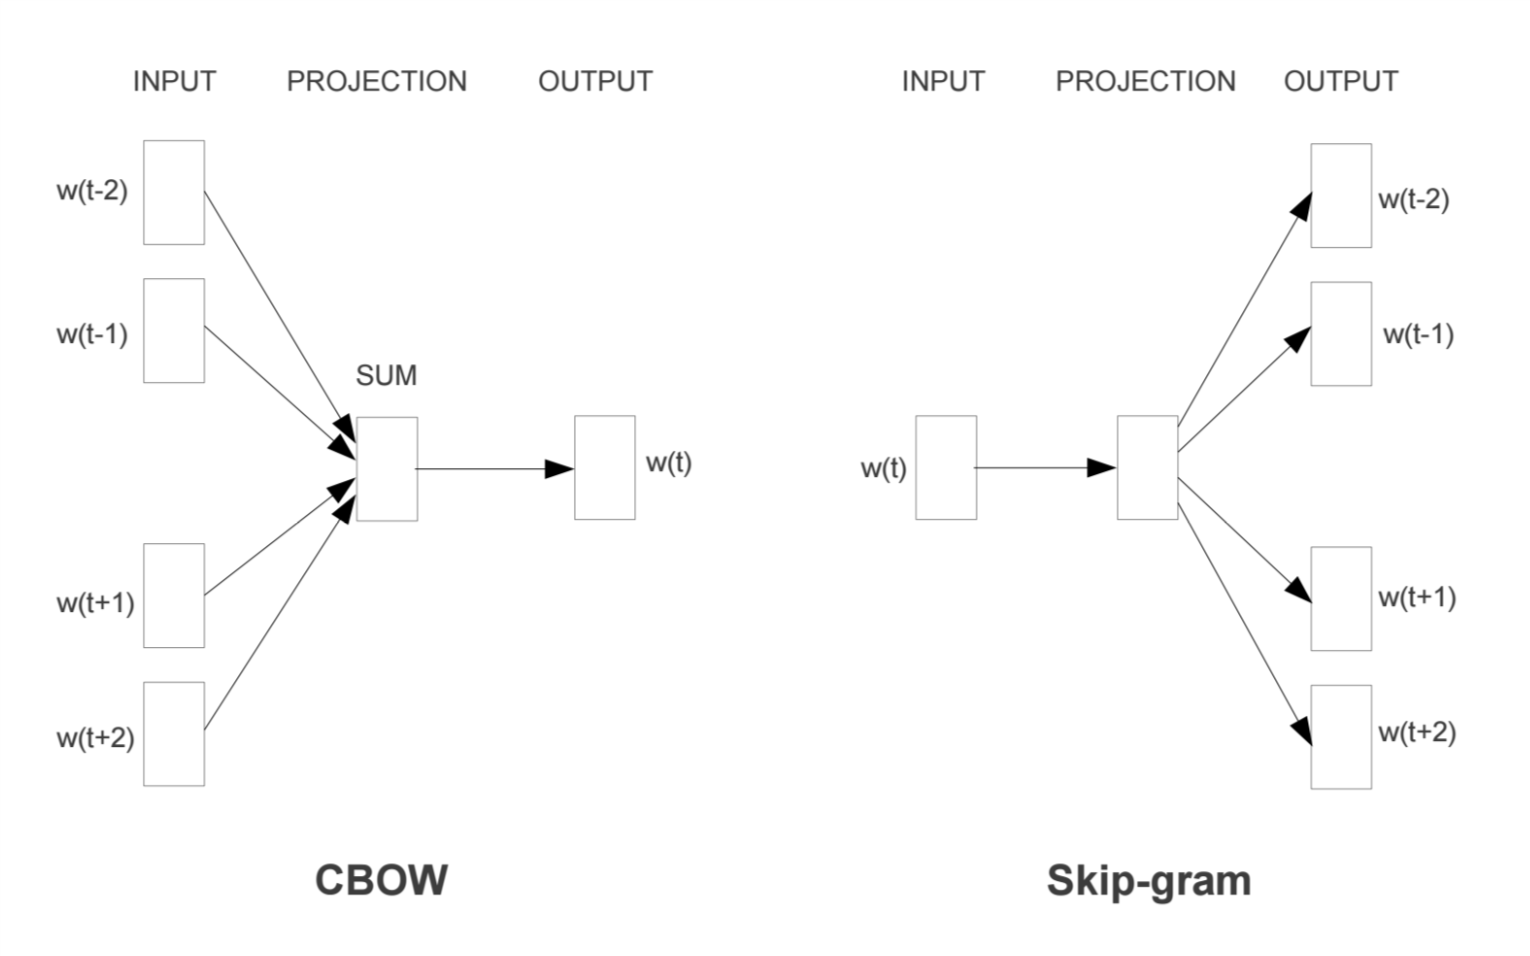
\includegraphics[width=0.85\linewidth]{images/word2vec}
	\caption{CBOW and Skip-gram architectures~\citep{mikolov2013efficient}}
	\label{fig:word2vec}
\end{figure}

Word2Vec has two architectures, namely Continuous Bags of Words (CBOW) and Skip-gram~\citep{mikolov2013efficient}, as illustrated in Figure~\ref{fig:word2vec}. In CBOW, the model learns to predict a word based on its neighboring words. Therefore, the input layer is represented with the bag-of-words. In contrast, Skip-gram architecture aims to predict the neighboring words based on a given word. The advantage of CBOW is that it can be used for training a huge amount of data, while Skipgram is best for capturing the average co-occurance from two words from the data.

Both architectures mainly aims to build language model, however, one does not need the whole trained model for having the word embedding representation. Instead, one only needs to extract the weight matrix used for converting words into vectors from the model. This weight matrix is the word embedding model that we use for transforming the words into dense vectors.

\section{Deep Learning}
Deep learning is a branch of machine learning that has multiple layers inside the model. Deep learning is able to extract implicit features in a high, abstract level~\citep{lecun2015deep}. Deep learning model has proved to produce robust performance in a variety of reserach, including computer vision and natural language processing.

Deep learning is basically a neural networks model with deeper hidden units. Neural networks model is based on how the neuron works inside human brain. Neurons with deep hidden units are then able to extract features in a abstract level~\citep{bengio2007scaling}. The deep learning structure consists of input layer, hidden layer, and output layer. The input layer is where the data being fed into the model, while output layer is the result of the model. The important layer here is the hidden layer in which a linear and/or non-linear functions are approximated in order to get the best predicted outputs.

Deep learning model has proved to give outstanding performances in supervised learning~\citep{Goodfellow-et-al-2016-Book}. A model with deeper layer will learn more implicit features out of the training data. There are a lot of deep learning architectures that have been proposed, one of which is the Recurrent Neural Networks~\citep{elman1990finding}. Each deep learning architecture is designed to fulfill specific computation needs.

\subsection{Recurrent Neural Networks}
Recurrent Neural Networks, shortened as RNN, is one of deep learning architectures designed for processing sequential data. There are some varieties of RNN, including the one proposed by~\cite{elman1990finding} and~\cite{jordan1986attractor}. Since it is designed for processing sequential data, it has a nature advantage for modeling the sequence labeling problem. Suppose that we have sequence of inputs, RNN will take each input in a time step $t$ to process it in a function. Figure~\ref{fig:simplernn} shows a general RNN.

\begin{figure}
	\centering
	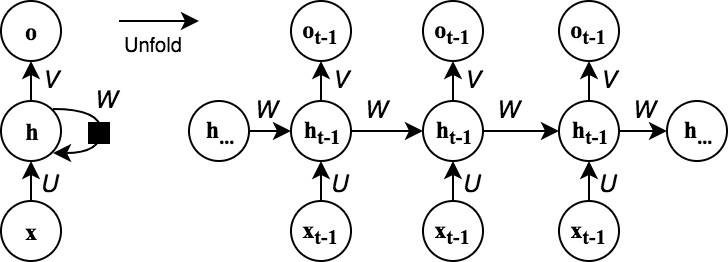
\includegraphics[width=0.80\linewidth]{images/RNNNew}
	\caption{A simple Recurrent Neural Networks (RNN). (left) folded RNN. (right) unfolded RNN}
	\label{fig:simplernn}
\end{figure}

The left picture illustrates the folded RNN model applied to all time steps. Note that the black rectangle represents one time step delay, meaning that that input is coming from the output of the previous time step. 

The right picture shows the unfolded RNN that is more intuitive since it visualizes the time steps. There are three layers in every time step t, which are input, hidden, and output layers. The input layer is for the input representations. In the hidden layer, it contains information from the input layer as well as those coming from hidden layers in the previous time steps. The output layer consists of the output of the model. These three layers are in a form of vectors. In every time step $t$, RNN has an input layer $ \mathbf{x_{t}} \in {\rm I\!R^{A}} $, hidden layer $ \mathbf{h_{t}} \in {\rm I\!R^{H}} $, and output layer $ \mathbf{o_{t}} \in {\rm I\!R^{B}} $. The values of $A$, $H$, and $B$ represent the length of the input vector, the number of unit in a hidden layer, and the length of the output vector, respectively. There are three parameters that will be trained, which are $U$, $V$, and $W.$ These parameters are the weight matrices for connecting two layers. $ U \in {\rm I\!R^{H \times A }}$ connects input layer with hidden layer (input-hidden), $ W \in {\rm I\!R^{H \times H}}$ connects hidden layer with the previous hidden layer (hidden-hidden), and $ V \in {\rm I\!R^{B \times H}}$ connects hidden layer with output layer (hidden-ouput). These parameters are time-distributed, meaning that they are shared across time steps. 

Every input layer $ \mathbf{x_{t}} $ is mapped into output layer $ \mathbf{o_{t}} $ in every time step $t$. In the middle of the process, the model calculates the hidden layer $ \mathbf{h_{t}} $ from two layers, $ \mathbf{x_{t}} $ and $ \mathbf{h_{t-1}} $. The output layer $ \mathbf{o_{t}} $ is then retrieved by performing a function to the hidden layer $\mathbf{h_{t}}$. The general equations for RNN are presented as follows:
\begin{equation}
\label{eq:rnnot}
\mathbf{o_{t}} = f2(V \cdot \mathbf{h_{t}} + \mathbf{c})
\end{equation}

\begin{equation}
\label{eq:rnnht}
\mathbf{h_{t}} = f1(U \cdot \mathbf{x_{t}} + W \cdot \mathbf{h_{t-1}} + \mathbf{b})
\end{equation}

Where $ \mathbf{h_{0}} = f1(U \cdot \mathbf{x_{0}}) $.

Note that there are two additional parameters to train, which are the bias vectors $\mathbf{b}$ and $\mathbf{c}$. In Equation~\ref{eq:rnnht}, the input $\mathbf{x_{t}}$ and $\mathbf{h_{t-1}}$ are weighted by matrices $U$ and $W$ respectively, added by a bias vector $\mathbf{b}$. The result is then inserted to an activation function $f1$ in order to produce hidden layer $\mathbf{h_{t}}$. In the Equation~\ref{eq:rnnot}, $\mathbf{h_{t}}$ is multiplied by the weight matrix $V$ and added by a bias vector $\mathbf{c}$ before being processed by the activation function $f2$ to produce $\mathbf{o_{t}}$. The examples of activation function $f1$ and $f2$ are tanh and softmax.

Based on this illustration, there are two main characteristics of RNN:
\begin{enumerate}
	\item It has a cycle in the graph for every time step. Hidden layer $\mathbf{h_{t-1}}$  will be one of the inputs for forming $\mathbf{h_{t}}$ .
	\item It has shared parameters across time steps.
\end{enumerate}

Figure~\ref{fig:fulrnn} illustrates a more complete RNN model on how it is being trained.

\begin{figure}
	\centering
	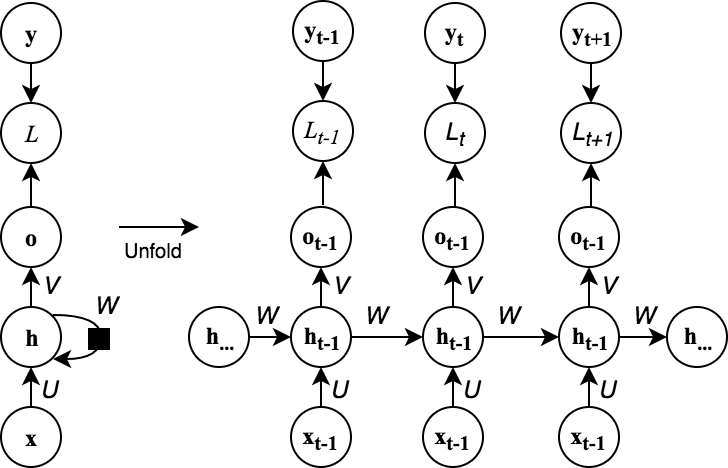
\includegraphics[width=0.80\linewidth]{images/RNNUnfoldNew}
	\caption{A Complete RNN on how it is being trained. (left) folded RNN. (right) unfolded RNN}
	\label{fig:fulrnn}
\end{figure}

The goal of training the model is to find the estimated values of parameters $W$, $U$, $V$, $\mathbf{b}$, and $\mathbf{c}$ which produce output $\mathbf{o_{t}}$ as close as the expected output $\mathbf{y_{t}}$ in the training data. 

The loss function $L$ measures the difference between the predicted output $\mathbf{o_{t}}$ and the expected output $\mathbf{y_{t}}$ in every time step t. The smaller the difference, the better the model. The machine thus has to minimize the result of loss function as small as possible. The parameters $W$, $U$, $V$, $\mathbf{b}$, and $\mathbf{c}$ are unknown in the beginning. At first, these parameters are initiated randomly. For every iteration, called epoch, the machine aims to learn the best values for each parameter.

The way to do so is by computing the gradient for each iteration. The idea behind computing the gradient values is to tell the model which parameter setting that brings it into smaller loss function result. By having this information, the machine then sets the better values for each parameter in the next iteration in order to reduce the loss function. From one iteration into another, the machine will find better parameter values to minimize the loss function. The learning method based on the gradient information is called optimization algorithm. Some optimization algorithms available are Adam~\citep{kingma2014adam}, and RMSProp~\citep{tieleman2012lecture}.

\subsection{Long Short-Term Memories}
Regular RNN has an issue called vanishing and exploding gradient problem. The RNN architecture repeatedly uses the same parameters for each time steps. Suppose that we use $W$ as the parameter for each time step between the hidden units. After $t$ time steps, the matrix would be multiplied $t$ times, hence it is the same as multiplying the hidden units with $W^{t}$~\citep{Goodfellow-et-al-2016-Book}. Assuming that $W$ has an eigen-decomposition $W = X \cdot diag(\lambda) \cdot X^{-1}$, $W^{t}$ is equal to:
\begin{equation}
W^{t} = (X \cdot diag(\lambda) \cdot X^{-1})^{t} = (X \cdot diag(\lambda)^{t} \cdot X^{-1})
\end{equation}

The eigenvalues $\lambda$ in $diag(\lambda)$ will either vanish if they are less than 1 in magnitude or explode if they are greater than 1 in magnitude. The gradient counted in each time step is aligned with the eigenvalues. Hence, the gradient may also vanish or explode. This is what we called as vanishing and exploding gradient problem. When the gradient vanishes, it is hard for the machine to find the direction to reduce the lost function. In the case of exploding gradient, the learning algorithm will become unstable.

To address this issue, there are solutions proposed such as simulated annealing and discrete error propagation~\citep{bengio1994learning}, time delays~\citep{lang1990time}, and hierarchical sequence compression~\citep{schmidhuber2007training}. Among these approaches, one of the most robust solutions is the Long Short Term Memories (LSTM)~\citep{hochreiter1997long}. 

The modification added in LSTM to address the issue is by using gates. It is basically RNN, but the nonlinear units in the hidden layer is replaced by the memory blocks. One nonlinear unit $tanh$ in RNN is replaced by more complex memory blocks in LSTM. Besides the hidden layer $\mathbf{h_{t}}$, LSTM also has $\mathbf{m_{t}}$ which is called memory cells.  The idea of LSTM is to learn when to forget or remember the memory from previous time steps through multiplicative gates. It thus prevents the vanishing and exploding gradient problem. For example, if the input gate is closed, then the memory will be unchanged.

Figure~\ref{fig:lstm} illustrates a one block memory in LSTM. There are three main gates, which are forget gate, input gate, and output gate. These gates are responsible to determine whether an information is added, kept, or deleted in a cell. Each gate has sigmoid layer and element-wise operations. The sigmoid layer converts the input into a probability between 0 and 1. This probability describes the gate behavior towards the input, whether to accept it (probability close to 1) or not (probability close to 0). 

\begin{figure}
	\centering
	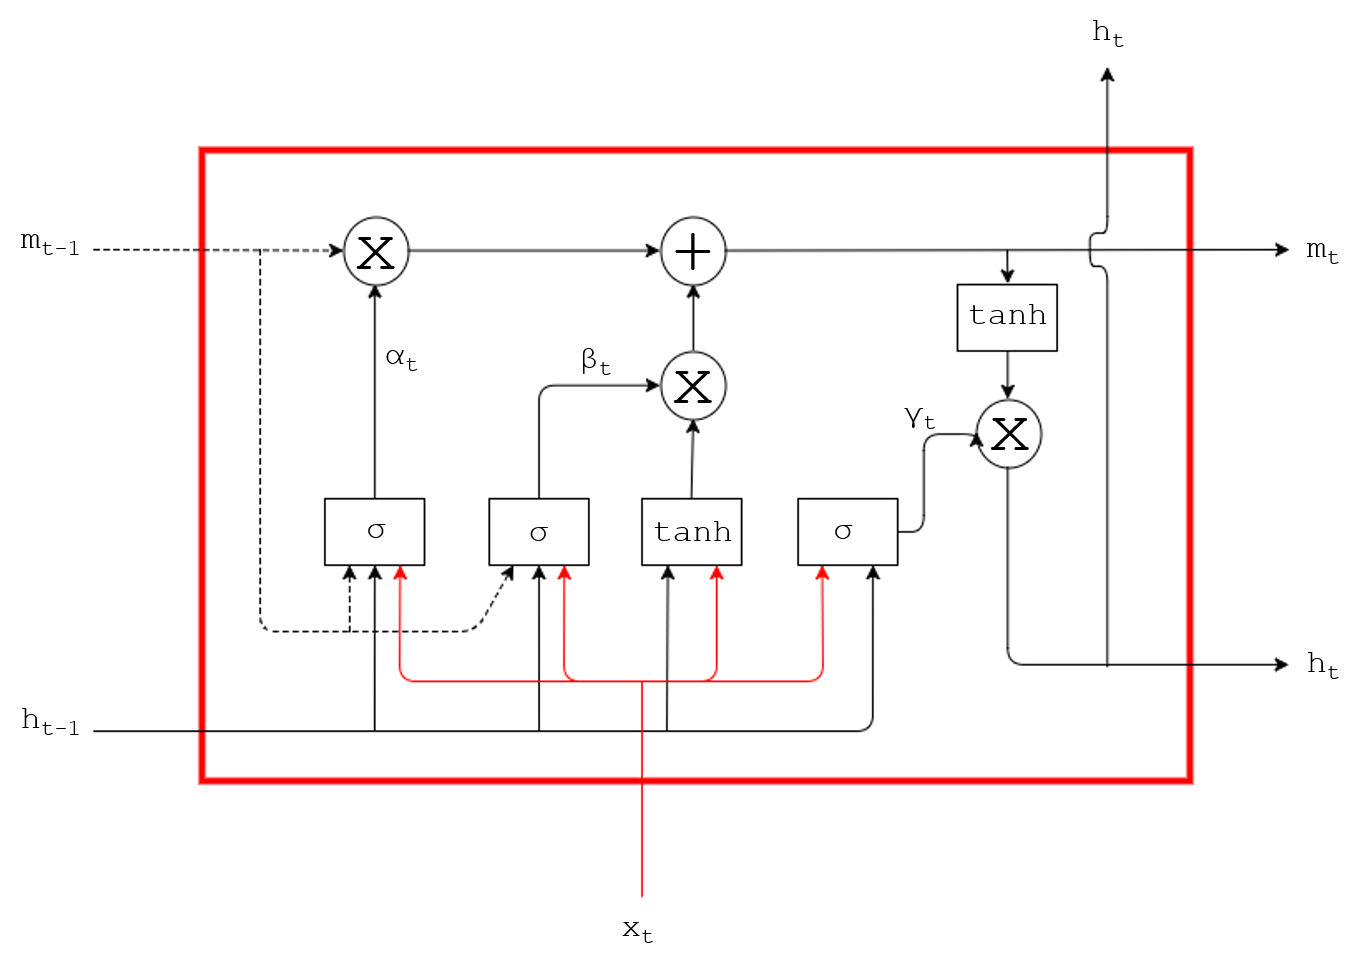
\includegraphics[width=1.0\linewidth]{images/lstm}
	\caption{One memory block in LSTM~\citep{skripsiwahid}}
	\label{fig:lstm}
\end{figure}

The equations of the sigmoid layers for each of the gates are explained as follows:
\begin{enumerate}
	\item \textit{Forget Gate}\\
	This gate is responsible to determine how much the information from the past should be kept in the memory. The equation of the forget gate is given as follows:
	\begin{equation}\label{eq:forget_lstm}
	\alpha_{t}=\sigma(W_{x\alpha}\cdot \mathbf{x_{t}}+W_{h\alpha}\cdot~\mathbf{h_{t-1}}+W_{m\alpha}\cdot~\mathbf{m_{t-1}})
	\end{equation}
	
	\item \textit{Input Gate}\\
	This gate is responsible to determine how much the current information x(t) should be kept in the memory. The equation of the input gate is given as follows:
	\begin{equation}\label{eq:input_lstm}
	\beta_{t}=\sigma(W_{x\beta}\cdot \mathbf{x_{t}}+W_{h\beta}\cdot~\mathbf{h_{t-1}}+W_{m\beta}\cdot~\mathbf{m_{t-1}})
	\end{equation}
	
	\item \textit{Output Gate}\\
	This gate is responsible to determine the output of a time step based on current cell state. The equation of the output gate is given as follows:
	\begin{equation}\label{eq:output_lstm}
	\gamma_{t}=\sigma(W_{x\gamma}\cdot \mathbf{x_{t}}+W_{h\gamma}\cdot~\mathbf{h_{t-1}}+W_{m\gamma}\cdot~\mathbf{m_{t-1}})
	\end{equation}
	
\end{enumerate}

In every time step $t$, the equations for computing cell state $\mathbf{m_{t}}$ and hidden layer $\mathbf{h_{t}}$ are presented as follows:
\begin{equation}\label{eq:mt}
\mathbf{m_{t}}=\alpha_{t} (\times) \mathbf{m_{t-1}} + \beta_{t} (\times) tanh(W_{xm} \cdot \mathbf{x_{t}} + W_{hm} \cdot \mathbf{h_{t-1}}))
\end{equation}
\begin{equation}\label{eq:ht}
\mathbf{h_{t}}=\gamma_{t} (\times) tanh(\mathbf{m_{t}})
\end{equation}

\section{Semantic Role Labeling}
Semantic role labeling (SRL) is a task in Natural Language Processing to assign semantic roles for each argument for each predicate in given input sentence~\citep{jurafsky2016speech}. In this section, the definition of semantic roles and the most commonly used annotation corpora for SRL are explained. In the end, the details on the semantic role labeling task are described.

\subsection{Semantic Roles}
Semantic roles are the representations that express the abstract role of the arguments of a predicate can take in the event~\citep{jurafsky2016speech}. When it comes to understanding natural language, one would want to understand the events and their participants of a given input sentence. In this case, the events refer to the predicate and the participants refer to the argument. Table~\ref{tab:examplesrl1} illustrates the connection between a predicate and its arguments.

\begin{table}
	\centering
	\caption{An example predicate and its arguments}
	\label{tab:examplesrl1}
	\begin{tabular}{|ccc|}
		\hline
		\underline{Andy} & \underline{eats} & \underline{fried chicken} \\
		\textsc{Argument} & \textsc{Predicate} & \textsc{Argument} \\
		\hline
	\end{tabular}
\end{table}

In this example, "eat" is the predicate with "Andy" and "fried chicken" as its argument. With this point of view, the predicate can be seen as the center of the sentence, followed by the arguments that depend on it.

Knowing the predicate and its arguments is not enough to understand the sentence since the roles of the arguments towards the predicate are unknown. In the previous example, it will be more meaningful to differentiate that "Andy" is the \textsc{Eater} and fried chicken is the \textsc{EatenThing}. \textsc{Eater} and \textsc{EatenThing} are the examples of semantic roles for the predicate "eat". These semantic roles could be used to identify the roles of the arguments regardless its position in the sentence. The previous example could be represented in two ways, as presented in Table~\ref{tab:examplesrl2}

\begin{table}
	\centering
	\caption{Examples of a predicate and its deep roles}
	\label{tab:examplesrl2}
	\begin{tabular}{|ccc|}
		\hline
		\underline{Andy} & \underline{eats} & \underline{fried chicken} \\
		\textsc{Eater} & \textsc{Predicate} & \textsc{EatenThing} \\
		\hline
		\underline{The fried chicken} & is \underline{eaten} & by \underline{Andy} \\
		\textsc{EatenThing} & \textsc{Predicate} & \textsc{Eater} \\
		\hline
	\end{tabular}
\end{table}

Both sentences represent the role of "Andy" and "fried chicken" as \textsc{Eater} and \textsc{EatenThing} respectively, regardless of their position in the sentence as a subject or object.

There are many ways to define such semantic roles. From the example above, the semantic roles are very specific for its predicate, known as deep roles~\citep{jurafsky2016speech}. \textsc{Eater} and \textsc{EatenThing} are the semantic roles for the predicate "eat", \textsc{Kicker} and \textsc{KickedThing} are the semantic roles for the predicate "kick", and so on. In order to further knowing more about the semantics of these arguments, the semantic roles could be generalized into more abstract roles. \textsc{Eater} and \textsc{Kicker} have something in common: they are volitional actors having direct causal responsibility for the predicate. Volitional means that the actors have the willing to decide on and commit to a particular action that they do. For this reason, thematic roles are introduced as a set of semantic roles designed to capture semantic commonality between \textsc{Eater} and \textsc{Kicker}~\citep{jurafsky2016speech}. With this in mind, \textsc{Eater} and \textsc{Kicker} can be represented as AGENT, which represents the abstract concept that is a volitional causer of an event (or predicate). On the other hand, \textsc{EatenThing} and \textsc{KickedThing} both represent the direct objects that are affected by the event. The thematic role for \textsc{EatenThing} and \textsc{KickedThing} is THEME.

Table~\ref{tab:examplesrl3} describes the thematic roles often used across computational papers~\citep{jurafsky2016speech}
\begin{table}
	\scriptsize
	\centering
	\caption{Examples of thematic roles~\citep{jurafsky2016speech}}
	\label{tab:examplesrl3}
	\begin{tabular}{lll}
		\hline
		\textbf{Thematic Role} & \textbf{Definition} & \textbf{Example} \\
		\hline
		AGENT & The volitional causer of an event & \underline{The waiter} spilled the soup \\
		EXPERIENCER & The experiencer of an event & \underline{John} has a headache \\
		FORCE & The non-volitional causer of the event & \underline{The wind} blows debris \\
		THEME & The participant directly affected by an event & Benjamin Franklin broke \underline{the ice} \\
		RESULT & The end product of an event & The city built \underline{a requlation-size baseball diamond} \\
		CONTENT & The content of a propositional event & Mona asked \underline{"Did you met Mary Ann?"} \\
		INSTRUMENT & An instrument used in an event & He stunned catfish with \underline{a shocking device} \\
		BENEFICIARY & The beneficiary of an event & Ann Callahan makes hotel reservations for \underline{her boss} \\
		SOURCE & The origin of the object of a transfer event & I flew in \underline{from Boston} \\
		GOAL & The destination of an object of a transfer event & I drove \underline{to Portland} \\
		\hline
	\end{tabular}

\end{table}

AGENT and EXPERIENCER represent the volitonal causer of an event and the experiencer of an event, respectively. While AGENT is volitional, the non-volitional causer of an event is called FORCE. Furthermore, THEME and RESULT are the participant directly affected by an event and the end product of an event, respectively. BENEFICIARY represents the beneficiary of an event. CONTENT describes the content of a propositional event. An instrument used in an event is called INSTRUMENT. For location, there are SOURCE and GOAL which represent the origin and the destination of an object of a transfer event.


\subsection{Annotation Corpus}
There are available annotated corpus for SRL consisting of sentences labeled with semantic roles. Researchers are using these annotated corpus for building supervised machine learning model for SRL. The two most commonly used annotation corpus for SRL are Proposition Bank and FrameNet.

\subsubsection{Proposition Bank}
Proposition Bank~\citep{kingsbury2002treebank}, shortened as PropBank, is a corpus in which sentences are annotated with semantic roles. PropBank corpus is available for many languages, such as English, Chinese, Hindi, Arabic, Finnish, and Portuguese. The main approach used for its semantic roles grouping is based on proto-roles and verb-specific semantic roles. Every verb sense has its set of semantic roles with argument numbers rather than names, for example: Arg0, Arg1. Arg2, etc. Usually, Arg0 represents PROTO-AGENT while Arg1 represents PROTO-PATIENT. Other argument number representations may vary based on each verb sense.

Both PROTO-AGENT and PROTO-PATIENT are generalized roles that describe roughly agent-like and roughly patient-like meanings, respectively~\citep{jurafsky2016speech}. Both roles are defined by heuristic features that describe more agent-like or more patient-like meanings. For instance, when the argument has more agent-like properties (causing an event, causing a change of state of other participant, being volitionally involved in the event) the likelihood that the argument can be labeled as PROTO-AGENT will be greater. On the other hand, the more an argument has patient-like properties (causally affected by another participant, undergoing change of state), the bigger the likelihood that the argument to be labeled as PROTO-PATIENT. 

The PropBank entries are called frame files. One example of the frame files for one sense of verb eat is presented as follows.
\\
\fbox{%
	\parbox{1.0\linewidth}{%
		\textbf{Frame File:}\\
		\textit{Eat.01}\\
		Arg0: Eater\\
		Arg1: Things Eaten\\
		Arg2: Instrument used\\
		\\
		\textit{Example:}\\
		Ex1: [Arg0 Andy] eats [Arg1 fried chicken] [Arg2 with spoon]\\
		Ex2: [Arg1 That fried chicken] is eaten by [Arg0 Andy] [Arg2 with spoon]
	}%
}
\\

For verb sense Eat.01, Arg0 acts as the Eater (PROTO-AGENT), and Arg1 represents the Things Eaten (PROTO-PATIENT). As we can see from the example above, we can infer the commonality between examples Ex1 and Ex2 regardless its structure, be it in a passive or active voice. In both examples, Andy is the Eater and fried chicken is the Things Eaten. In this frame file, there is also another argument, Arg2, that represents the instrument used by the Eater. In example Ex1 and Ex2, the instrument is spoon.

Other non-numbered arguments are available in PropBank, the so-called ArgMs, representing modifiers that could be used across frame files. Some examples of ArgMS include:
\\
\fbox{%
	\parbox{1.0\linewidth}{%
		TMP: When?\\
		LOC: Where?\\
		DIR: Where to/from?\\
	}%
}
\\

The next annotation corpus is called FrameNet which has different approach on how to group the set of semantic roles. Instead of using verb-specific, it uses frame-specific grouping.

\subsubsection{FrameNet}
FrameNet~\citep{baker1998berkeley} is an annotation corpus for semantic roles that are specific to a frame. In PropBank, the semantic roles are defined based on each sense of a verb. In contrast, a frame in FrameNet could include more than one predicate (verbs or nouns) that have the same background context. Each frame consists of two elements: 1.) A set of semantic roles related to this frame, and 2.) A set of predicates using the respective semantic roles.

One example is a frame called $\mathbf{change\_position\_on\_a\_scale}$~\citep{jurafsky2016speech} defined as:
\\
\fbox{%
	\parbox{1.0\linewidth}{%
		\texttt{This frame consists of words that indicate the change of an Item's position on a scale (the Attribute) from a starting point (Initial value) to an end point (Final value).} \\
	}%
}
\\

The set of semantic roles for a frame is divided into two roles: Core roles and Non-Core Roles. Core Roles are specific to a frame while Non-Core Roles are more general across frames (like ArgMs in PropBank). The set of semantic roles of the frame $\mathbf{change\_position\_on\_a\_scale}$ is explained as follows.
\\
\fbox{%
	\parbox{1.0\linewidth}{%
		\textbf{Core Roles}\\
		ITEM: The entity that has a position on the scale.\\
		ATTRIBUTE: The ATTRIBUTE is a scalar property that the ITEM possesses\\
		DIFFERENCE: The distance by which an ITEM changes its position on the scale. FINAL STATE: A description that presents the ITEM's state after the change in the ATTRIBUTE's value as an independent predication.\\
		FINAL VALUE: The position on the scale where the ITEM ends up. \\
		INITIAL STATE: A description that presents the ITEM's state before the change in the ATTRIBUTE's value as an independent predication.\\
		INITIAL VALUE:The initial position on the scale from which the ITEM moves away. \\
		VALUE RANGE: A portion of the scale, typically identified by its end points, along which the values of the ATTRIBUTE fluctuate. \\
		\\
		\textbf{Non-Core Roles}\\
		DURATION: The length of time over which the change takes place.\\
		SPEED: 	The rate of change of the VALUE.\\
	}%
}
\\

For instance, the possible predicates of the frame change position on a scale are: \textit{rose, increase, fell}.

The example of semantic roles of the frame $\mathbf{change\_position\_on\_a\_scale}$ can be seen as follows:

[ITEM Oil] rose [ATTRIBUTE in price] [DIFFERENCE by 2\%]. 

[ITEM It] has increased [FINAL STATE to having them 1 day a month]. 

[ITEM Microsoft shares] fell [FINAL VALUE to 7 5/8]. 

[ITEM Colon cancer incidence] fell [DIFFERENCE by 50\%] [GROUP among men]

a steady increase [INITIAL VALUE from 9.5] [FINAL VALUE to 14.3] [ITEM in dividends]

a [DIFFERENCE 5\%] [ITEM dividend] increase... 

As we can see from the examples above, \textit{rose}, \textit{fell}, and \textit{increase} have the same set of semantic roles under the frame $\mathbf{change\_position\_on\_a\_scale}$. Instead of defining the semantic roles for each verb sense one by one, FrameNet groups predicates (not limited to verbs) that have same semantic roles as one frame.
%\subsection{Problem Definitions}
%Semantic Role Labeling (SRL) is one of Natural Language Processing task which aims to automatically assign semantic roles for each constituent (argument) for each predicate in a sentence~\citep{jurafsky2016speech}. Current approach to solve this task is by using supervised machine learning. Given a labeled data, the machine learns from it and builds a generalization model. Researches often used PropBank or FrameNet corpus as the sources of annotated data. In this section, we describe the approaches to define the problem of SRL task, followed by the common features used for building supervised model for SRL.
%
%There are two ways to see SRL problem, either as Classification or Sequence Labeling problem. Classification approach assigns semantic roles for each word independently. Meanwhile, Sequence Labeling approach traverses from assigning semantic role for the first word until the last one in a sentence sequentially. In Sequence Labeing, the next label (semantic role) prediction of time step t is dependent to labels predicted on previous time steps (1..t-1).
%
%In classification approach approach, suppose that we have an input of \textit{n} words $w = (w_{1}, w_{2}, ..., w_{n})$. Each vector $w_{i}$ is classified into a label $y_{i}$ that represents the semantic role. The probabilities of the label in each time step $i$ is described as follows.
%\begin{equation}
%P(y_{i}|w_{i})
%\end{equation}
%
%In sequence labeling approach, suppose that we have an input of \textit{n} words $w = (w_{1}, w_{2}, ..., w_{n})$, the goal is to find the best label sequence $y = (y_{1}, y_{2}, ..., y_{n})$, with $y_{i}$ representing the semantic roles. The probabilities of the label in each time step $i$ is described as follows.
%\begin{equation}
%P(y_{i}|w_{i-l}, ..., w_{i+l},y_{i-l}, ..., y_{i+l})
%\end{equation}
%
%whereby \textit{l} is a small number. 

\subsection{Common Features for SRL}
The first set of features for SRL is proposed by~\cite{gildea2002automatic}. They are the first ones who used supervised machine learning approach to solve SRL. Over the years, many research proposed new set of features to improve the result. The common features used for solving SRL task are presented as follows~\citep{jurafsky2016speech}.
\begin{enumerate}
	\item The predicate.\\
	Usually in a form of verb.
	\item The phrase type of the constituent.\\
	NP, PP, etc
	\item The headword of the constituent.\\
	Example: The black \textit{bird}.
	\item The headword part of speech of the constituent. \\
	Example: The black \textit{bird}. POS of \textit{bird} is Noun.
	\item The path of the parse tree from constituent to predicate. \\
	This is to represent the grammatical relationships between the constituent and the predicate.
	Example: NP-S-VP-VBD
	\item The voice of the clause, active or passive.\\
	Example: I eat chicken rice (active), Chicken rice is eaten by me (passive).
	\item The binary linear position of the constituent from the predicate.\\
	Could be before or after the predicate.
	\item The subcategorization of the predicate\\
	Set of arguments that appear in the verb phrase VP.
	Example: NP and PP in 'VP -> VBD NP PP'
	\item The named entity type of the constituent\\
	Example: Organization, Person, Location
	\item The first and last words of the constituent.
\end{enumerate}

There are also other additional features that could be used for SRL, such as sets of n-grams inside the constituent. Another variation is to use dependency parser instead of syntactic parser for extracting features.

\subsection{Historical Perspectives}
SRL can be seen as either a classification or sequence labeling problem. The earlier research on SRL was conducted with the classification approach, meaning that each argument is being predicted independently from the others. Those research focused on how to extract meaningful features out of syntactic parsers~\citep{gildea2002automatic, gildea2002necessity, pradhan2005semantic}, such as the path to predicate and constituent type. This syntactic information plays a pivotal role in solving SRL problem~\citep{punyakanok2008importance} as it addresses SRL's long distance dependency~\citep{zhou2015end}. Thus, traditional SRL system heavily depends on the quality of the parsers. The analysis done by~\cite{pradhan2005semantic} shows that most errors of the SRL system were caused by the parser's error. In addition, those parsers are costly to build, since it needs linguistic experts to annotate the data. If we want to create an SRL system on another language, one should build a new parser all over again for it~\citep{zhou2015end}.

In order to minimize the number of hand-crafted features, ~\cite{collobert2011natural} utilized deep learning for solving NLP tasks including Part-of-Speech Tagging (POS), Chunking (CHUNK), Named Entity Recognition (NER), and Semantic Role Labeling (SRL) with classification approach. The research aimed to prevent using any task-specific feature in order to achieve state-of-the-art performance. The word embedding is used as the main feature across tasks, combined with Convolutional Neural Networks (CNN) architecture to train the model. They achieve promising results for the POS Tagging, Chunking and NER, while for SRL features from the parsers are still needed to achieve competitive results.

Different from the previous works,~\cite{zhou2015end} view SRL as a sequence labeling problem in which the arguments are labeled sequentially instead of independently. They proposed an end-to-end learning of SRL using Deep Bi-Directional Long Short-Term Memories (DB-LSTM), with word embedding as the main feature. Their analysis suggests that the DB-LSTM model implicitly extracts the syntactic information over the sentences and thus, syntactic parser is not needed. The research result outperforms the previous state-of-the-art traditional SRL systems as it achieves F1 score of 81,07\%. The research also shows that the performance of the sequence labeling approach using DB-LSTM is better than the classification approach using CNN, since the DB-LSTM can extract syntactic information implicitly.

%While many of the previous works studied SRL on formal language, our research aims to explore SRL on conversational language, which is still under-resourced. We thus introduce a new set of semantic roles for this language type. Furthermore, we propose a new architecture named Context-Aware Bi-Directional Long Short-Term Memories, designed with attention mechanism in order to capture context information of the sentence at a higher level.

% OR THIS ONE, ELLABORATE BOTH %
%Previous research have found useful to use RNN for NLP task Semantic Role Labeling (SRL). Before we discuss about the use of RNN on SRL, we describe the historical perspective of solving SRL with supervised machine learning. We divide the historical perspective based on SRL systems without and with deep learning.
%
%The non-deep learning approach uses specific hand-crafted features for SRL, which mainly depend on syntactic or dependency parser as explained in section 2.XX. It started from Gildea et. Al (2002) who firstly build supervised machine learning model for SRL. The goal of the research was to create the first shallow semantic role parser which is not domain specific, since at that time all the semantic roles research were too domain specific. The features used are extracted from the syntactic tree Collins Parser (XX, 1997), such as Phrase Type, Parse tree path, voice, and head word. Then the predicate of a sentence is also added as a feature. The research used semantic role annotation based on FrameNet. The algorithm used was statistical classifier with backoff approach. The result is 65\% precision and 61\% recall.
%
%Then, Gildea et al (2002) continues the research to quantify the effect of parser accuracy on SRL system’s performance. The research also examines whether a flatter “chunked” representation (which is less costly) of the input can be as effective as syntactic tree parser. The data used is from PropBank dataset, since it is from Wall Street Journal corpus that has a gold-standard syntactic parse trees for the entire dataset from the Penn Treebank Project. The finding shows that the parser accuracy affects the SRL system, since it is seen that the system with gold-standard parse tree impacts directly to build a better SRL system. Hence, the syntactic parser is an integral intermediary model to build a robust SRL system. If the parser is not good, one would not get a good SRL system.
%
%Surdeanu et al (2003) proposed a new set of features for SRL system, such as POS Tag of Head Word, POS Tag of content word, and Named Entity Class of Content Word. They use inductive learning through decision trees C5 for the algorithm.
%
%Xue et al (2004) aims to explore more information extracted from the parse tree in order to propose new set of features crafted to improve SRL. In their research, there are three steps for the model, pruning, argument identification, and argument classification. Pruning filters out constituents that are clearly not semantic arguments to the predicate. Argument identification classifies candidates as either semantic arguments or non arguments. Argument classification then runs a multi-category classifier to classify the constituents with semantic roles. The features proposed for the argument classification are syntactic frame, lexicalized constituent type, lexicalized head word, and the head of Preposition Phrase parent.
%
%Since the source of SRL system errors mostly based on syntactic parser’s error, Pradhan et al (2005) combines features from different syntactic parsers (Charniak parser and Collins Parser). The idea of combining two parser is that they train separate SRL systems for each tree parser. The role output from these two systems is used as additional features in a SRL system using flat syntactic view. They then use SVM classifier to train SRL based on PropBank data.
%
%Aside from using syntactic parse tree like Charniak or Collins parser, one can build SRL system by extracting features from dependency parser. Some of the features extracted are word property, syntactic connection, semantic connection, and dependency path.
%
%The drawbacks of using the non-deep learning approach are 1.) building syntactic or dependency parsers is costly, 2.) the SRL system hardly depends on the robustness of the parsers. Building tree parsers is costly because it is language-dependent and it needs experts in each language to create it. When we move to another language, we have to build these parsers for the new language from scratch. Not to mention a new problem arises when such parsers are not robust, hence creating error propagation in our SRL system. The analysis in Pradhan et al., (2005) says that the major source of errors in SRL system comes from the errors of the syntactic parsers from which we extract the features.
%
%To address this issue, Collobert et al. (20XX) firstly introduced the use of deep learning for SRL and other core NLP tasks such as POS Tagging and Chunking. They use Convolutional Neural Network (CNN) with no task-specific features for the system. For example, in non-deep learning approach, we use POS Tagging features for Chunking, and we use both of which as the features for SRL. Instead, the main feature used in this research is word embedding. As explained in the previous section, word embedding model converts words to vectors. The word vectors then are fed into CNN architecture. However, though the model achieved state-of-the-art performances for POS Tagging and Chungking, that is not the case for SRL. For SRL, it is still needed to use features from the tree parser to achieve robust performance.
%
%Zhou et al., (2015) proposed new architecture for the SRL system. Instead of seeing the SRL as a classification problem like the previous research including Collobert’s, Zhou considers SRL as the sequence labeling problem. Hence, the suitable architecture for such problem is Recurrent Neural Networks (RNN). In their research, a more specific RNN architecture is used, which is Long Short Term Memories (LSTM) in order to prevent the vanishing and exploding gradient problem in RNN. They used the deep bi-directional LSTM. The “deep” is for extracting more hidden features and the “bi-directional” is for extracting information from the past and future. On top of the LSTM architecture, they used Conditional Random Field (CRF) for the output layer. For the word representation, they also used word embedding as one of the main features, along with predicate and context predicate. Our research is mainly inspired by this research.

% PUNYA WAHID %

%\section{Deep Learning}
%\textit{Deep Learning}, atau disebut juga \textit{deep structured learning, hierarchical learning,} dan \textit{deep machine learning} merupakan salah satu cabang dalam \textit{machine learning} yang model komputasinya terdiri dari beberapa layer. \textit{Deep learning} mampu mempelajari dan mengekstrak representasi data/fitur secara otomatis pada abtraksi tingkat tinggi \citep{lecun2015deep}. Model tersebut memberikan hasil yang sangat baik dalam penelitan di berbagai bidang seperti \textit{speech recognition}, \textit{object detection}, \textit{sequence labeling} dan lain sebagainya.  
%
%Struktur pembelajaran pada \textit{deep learning} berbentuk hierarki karena termotivasi dari bagaimana neokorteks pada otak maunusia bekerja secara mendalam. Neokorteks tersebut melakukan proses pemelajaran berlayer dan secara otomatis mampu mengketrak fitur dan melakukan abstraksi dari \textit{resource} yang diberikan \citep{bengio2007scaling}. Struktur tersebut terdiri atas \textit{input layer}, \textit{hidden layer} dan \textit{output layer}. \textit{Input layer} memiliki fungsi sebagai tempat masuknya data yang akan dipelajari oleh model. \textit{Hidden layer} melakukan aproksimasi fungsi untuk mendapatkan target dari data \textit{training} yang diberikan. Disebut \textit{hidden layer} karena pada layer ini, \textit{output} tidak bisa kita lihat \citep{Goodfellow-et-al-2016-Book}. \textit{Hidden layer} inilah yang menjadi \textit{key role} dalam \textit{deep learning}. Sedangkan \textit{output layer} merupakan layer untuk mengembalikan target yang diinginkan.
%
%\textit{Deep learning} ini mampu memberikan model yanng memiliki performa sangat baik dalam \textit{supervised learning} \citep{Goodfellow-et-al-2016-Book}. Dengan menambahkan lebih banyak layer dan unit di dalam layer, \textit{deep network} dapat merepresentasikan fungsi dengan kompleksitas yang tinggi. Secara umum, \textit{deep learning} memetakan \textit{input vector} ke \textit{output vector}. Walaupun hal ini mudah dilakukan oleh manusia secar manual, namun untuk \textit{dataset} yang sangat besar, tentu hal ini tidak mungkin dilakukan. Ada banyak macam model \textit{Deep Learning} yang sesuai dengan kebutuhan komputasi, seperti \textit{Deep Belief Network} \citep{hinton2006fast}, \textit{Recurrent Neural Networks} \citep{elman1990finding}, \textit{Long Short Term Memory} \citep{hochreiter1997long}, \textit{Restricted Boltzman Machine} \citep{pennington2014glove} dan lain sebagainya. 

%\section{Recurrent Neural Networks}\label{sec:rnns}
%
%\textit{Recurrent neural networks} (RNNs) merupakan merupakan salah satu arsitektur \textit{Deep Learning} yang memiliki koneksi siklik \citep{graves2012neural}. RNNs memiliki \textit{neuron} yang terkoneksi dengan \textit{neuron} lain sehingga membentuk \textit{loop} umpan balik (\cite{haykin2009neural}), tidak seperti \textit{feedforward neural network} (FNNs) dimana aliran informasi hanya berjalan searah. RNNs memungkinkan \iob~yang dihasilkan akan menjadi \ioa~untuk menghasilkan \iob~yang lain. Hal ini menyebabkan perilaku RNNs tidak hanya bergantung pada \ioa~saat ini saja, namun juga bergantung pada \iob~sebelumya. Oleh karena itu, RNNs memiliki kemampuan yang sangat bagus sebagai model dalam permasalahan \textit{sequence data} dibandingkan dengan FNNs. RNNs sendiri memiliki kemampuan yang sangat bagus dalam beberapa \textit{task} terkait \textit{sequence data}, seperti \textit{language model} (\cite{mikolov2010recurrent}) dan \textit{speech recognition} (\cite{graves2013speech}).
%
%Dibandingkan dengan FNNs, RNNs memiliki beberapa kelebihan \citep{mikolov2010recurrent}, yaitu:
%\begin{enumerate}
%	\item Pada RNNs, kata-kata sebelumnya direpresentasikan dengan \textit{recurrent connections}, sehingga RNNs dapat menyimpan informasi kata sebelumnya dalam jumlah tak hingga. FNNs tidak bisa secara alami memodelkan hubungan kontekstual antara sebuah kata dengan kata-kata pada posisi sebelumnya dan representasi kata sebelumnya berupa konteks dari $ n-1 $ kata. Oleh karena itu, FNNs terbatas dalam penyimpanan informasi kata sebelumnya terbatas seperti pada model \textit{n-gram}.
%	\item RNNs dapat melakukan kompresi keseluruhan riwayat kata menjadi ruang dimensi yang lebih kecil, sedangkan FNNs melakukan kompresi/proyeksi hanya dengan sebuah kata saja.
%\end{enumerate}


%!TEX root = skripsi.tex
%-----------------------------------------------------------------------------%
\chapter{\babTiga}\label{bab:tiga}
%-----------------------------------------------------------------------------%
%-----------------------------------------------------------------------------%
% Ide, model matematik, rumus, fitur, jangan m=ngomongin teknologi (java, keras, dll), word2vec boleh %
Pada bab ini \saya~akan menjelaskan metodologi penelitian yang \saya~gunakan. Metodologi penelitian yang dilakukan meliputi tahap pengumpulan data, pra-pemrosesan data, pelabelan data, pengembangan model, eksperimen dan evaluasi.

\section{Gambaran Umum Pengembangan Metodologi}
Penelitian ini bertujuan untuk membuat sebuah model yang mampu memberikan label entitas kesehatan pada suatu dokumen. Seperti yang telah dijelaskan pada bab sebelumnya, terdapat banyak entitas kesehatan yang dapat digunakan sebagai target pelabelan. Oleh karena itu, untuk mempermudah penelitian ini \saya~menggunakan entitas-entitas yang diusulkan oleh \cite{skripsiKakRadit} dalam penelitiannya,  nama penyakit (\textit{\disease}), gejala penyakit (\textit{\symptom}), obat (\textit{\drug}) dan langkah penyembuhan (\textit{\treatment}).

Penelitian ini menggunakan dua buah korpus, yaitu korpus dari data dokumen teks kesehatan yang digunakan \cite{skripsiKakRadit} dan dokumen teks hasil pengumpulan yang dilakukan oleh \saya~pada situs kesehatan \textit{online}. Setelah itu \saya~melakukan pra-pemrosesan pada kedua data sebelum melakukan tahap selanjutnya. Untuk dokumen hasil pengumpulan dari forum, \saya~memberi label kesehatan secara manual dengan ketentuan pelabelan pada penelitian \cite{skripsiKakRadit}

Setelah tahap pengusulan model, terdapat 2 eksperimen yang \saya~lakukan, yaitu eksperimen untuk mendapatkan fitur diskriminatif yang mampu membuat model memiliki akurasi terbaik dan eksperimen untuk mendapatkan arsitektur RNNs yang membuat model menghasilkan akurasi tertinggi. Pada eksperimen pertama, \saya~mencoba beberapa fitur, seperti fitur yang diusulkan oleh \cite{skripsiKakRadit} (fitur \textit{its own word}, frasa, kamus (\textit{symptom}, \textit{disease}, \textit{treatment} dan \textit{drug}), kata pertama sebelum, dan fitur kata setelah. Pada eksperimen kedua, \saya~mencoba dua arsitektur RNNs, yaitu RNNs yang setiap \textit{input} digabung terlebih dahulu dengan meng-\textit{append} semua vektor fitur. Sedangkan RNNs yang kedua yaitu RNNs yang setiap kelompok fitur menjadi \textit{input} bagi masing-masing LSTMs, baru kemudian \textit{output} dari layer tersebut digabung.

Setelah melakukan eksperimen, \saya~melakukan evaluasi dari hasil yang didapatkan dengan menghitung nilai \textit{precission}, \textit{recall} dan \textit{F-measure} dari masing-masing entitas secara keseluruhan. Untuk mendapatkan rata-rata akurasi dari setiap eksperimen, \saya~melakukan \textit{10-fold cross validation} dengan cara membagi semua data menjadi 10 bagian, 9 bagian menjadi data \textit{training} dan 1 \textit{bagian} menjadi data \textit{testing}. Proses tersebut diulang sebanyak sepuluh kali sehingga masing-masing bagian data menjadi data \textit{testing}.
\begin{figure}
  \centering
  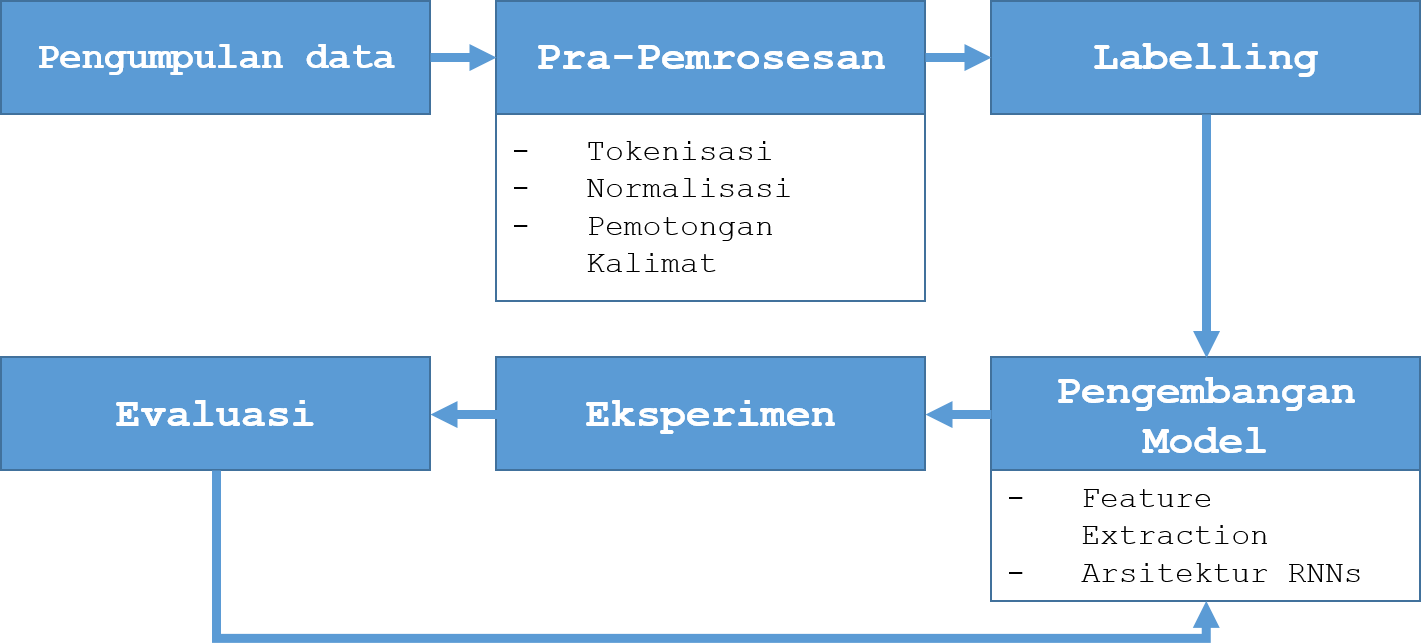
\includegraphics[width=\linewidth]{images/arsitektur}
  \caption{Diagram Gambaran Umum Metodologi yang Dilakukan}
  \label{fig:metodologi_penelitian}
\end{figure}

\section{Pengumpulan Data}
Pengumpulan data dilakukan dengan tujuan untuk mendapatkan data \textit{training} dan \textit{testing} yang akan digunakan sebagai \textit{resource} dalam melakukan \textit{training} dan evaluasi model \mer. Data yang dimaksud merupakan teks dari forum kesehatan \textit{online} dari berbagai sumber. Pada penelitian ini, \saya~menggunakan data penelitian \cite{skripsiKakRadit} dan data yang \saya~dapatkan dari hasil \textit{crawling} di forum kesehatan \textit{online}. Data yang \cite{skripsiKakRadit} diambil dari beberapa situs forum kesehatan \textit{online} dan sedangkan data yang \saya~unduh bersumber dari forum kesehatan \textit{online}.

\section{Pra-Pemrosesan}
Pra-pemrosesan dilakukan dengan tujuan supaya teks yang diberikan mampu dibaca oleh sistem \mer. Dalam tahap ini, ada tiga pekerjaan utama yang perlu dilakukan, yaitu:

\subsection{Pembersihan data}
Langkah ini dilakukan dengan tujuan untuk mempermudah proses POS \textit{tagging}. Selain itu, terdapat beberapa token yang berbeda sintaks namun memiliki jenis kata yang sama, misalnya token \textit{email}. Model hanya perlu tahu token tersebut merupakan email, tidak peduli pemilik email tersebut. Berikut merupakan beberapa langkah yang \saya~lakukan:
	
\begin{enumerate}
	\item menghapus karakter yang bukan merupakan karakter ASCII,
	\item mengganti token url menjadi kata "url", misalnya token tautan (\textit{www.alodokter.com/asma/pengobatan}) diganti menjadi token "url",
	\item mengganti token \textit{email} menjadi kata "email", misalnya sebuah alamat \textit{email} (\textit{wahid@domain.com}) diganti menjadi token "email",
	\item mengganti karakter "\_" menjadi token "underscore",
	\item mengganti karakter "\&" menjadi token "dan",
	\item mengganti karakter "\textless" dan "\textgreater" menjadi token "kurang dari" dan "lebih dari" dan
	\item mengganti karakter "/" menjadi token "atau".
\end{enumerate}
Pada langkah ini, \saya~tidak menghapus karakter tanda baca karena karakter tersebut memiliki fungsi pada sistem POS \textit{tagging} yang \saya~gunakan. Gambar \ref{fig:pembersihandata} merupakan contoh pembersihan data pada sebuah teks.
\begin{figure}
	\centering
	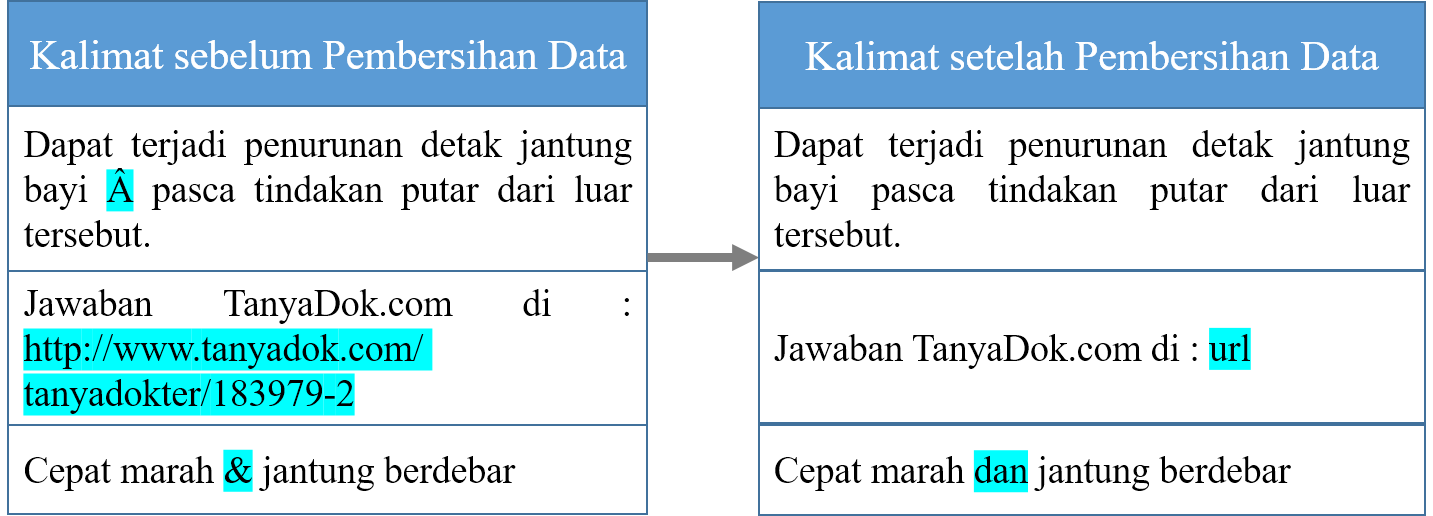
\includegraphics[width=\linewidth]{images/pembersihandata}
	\caption{Ilustrasi Pembersihan Data pada Kalimat}
	\label{fig:pembersihandata}
\end{figure}

	
\subsection{Tokenisasi}
Tokenisasi dilakukan untuk mendapatkan token yang paling tepat sebagai sebuah kata. Hal ini perlu dilakukan untuk menghindari beberapa kelompok token berbeda yang tergabung. Karakter abjad dengan karakter angka atau karakter abjad dengan karakter tanda baca dipisahkan berdasarkan kelompoknya. Misalnya token "pusing2" diubah menjadi "pusing 2". Pada tahap ini, \saya~melakukan pemisahan terhadap beberapa kelompok token, yaitu:
\begin{enumerate}
	\item <alfabet><numerik> menjadi <alfabet><spasi><numerik>
	\item <numerik><alfabet> menjadi <numerik><spasi><alfabet>
	\item <alfanumerik><non-alfanumerik> menjadi <alfanumerik><spasi><non-alfanumerik>
	\item <non-alfanumerik><alfanumerik> menjadi <non-alfanumerik><spasi><alfanumerik>
\end{enumerate}

Gambar \ref{fig:tokenisasi} berikut merupakan contoh tokenisasi pada sebuah teks.
\begin{figure}
	\centering
	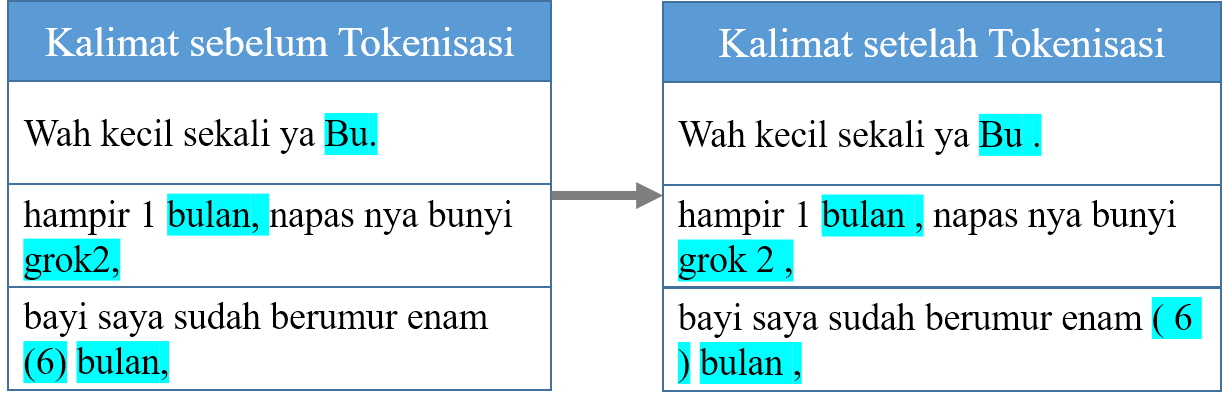
\includegraphics[width=\linewidth]{images/tokenisasi}
	\caption{Ilustrasi Tokenisasi pada Kalimat}
	\label{fig:tokenisasi}
\end{figure}

	
\subsection{Pemotongan kalimat}
Untuk menghindari jumlah token yang timpang dalam kalimat yang berbeda dan data yang \textit{sparse}, \saya~melakukan pemotongan kata dengan langkah-langkah sebagai berikut:
\begin{enumerate}
	\item memisahkan kalimat berdasarkan tanda baca (.!?,),
	\item apabila suatu kalimat memiliki jumlah kata yang sedikit (batasan minimal jumlah kata dalam sebuah kalimat yang \saya~gunakan adalah 10 kata), kalimat tersebut digabungkan dengan kalimat setelahnya.
\end{enumerate}

Gambar \ref{fig:pemotongan_kalimat} berikut merupakan contoh dari pemotongan kalimat pada sebuah teks.
\begin{figure}
	\centering
	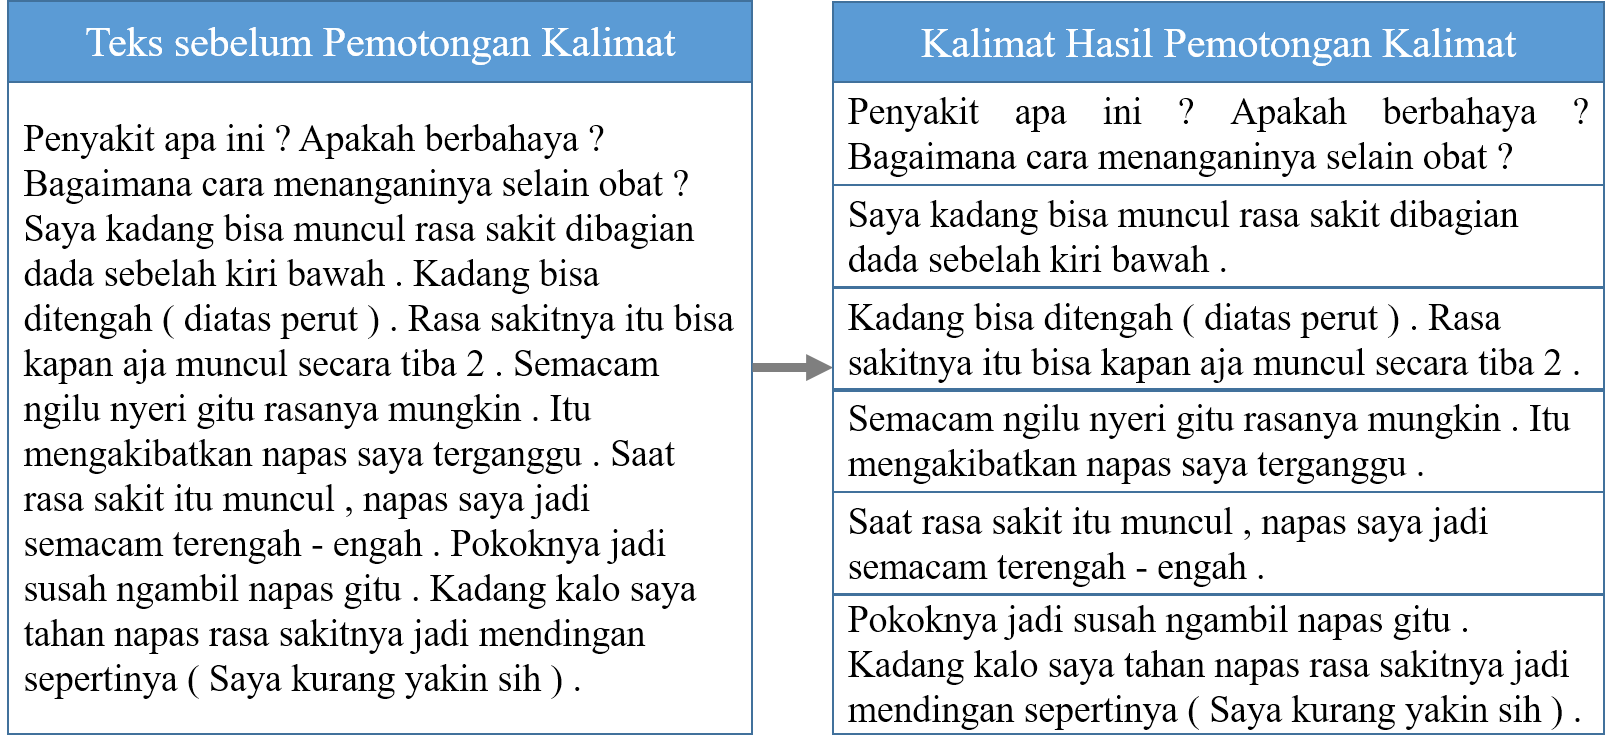
\includegraphics[width=\linewidth]{images/pemotongankalimat}
	\caption{Ilustrasi Pemotongan Kalimat pada suatu Teks}
	\label{fig:pemotongan_kalimat}
\end{figure}


\section{Pelabelan}
Pada tahap ini, \saya~melakukan pelabelan pada dokumen teks yang merupakan hasil pada tahap sebelumnya dengan label \disease, \symptom, \drug~dan \treatment. Berikut merupakan penjelasan dari masing-masing label:
\begin{enumerate}
	\item \Disease\\
	Entitas \disease~yang dimaksud pada penelitian ini yaitu nama dari suatu penyakit. Penyakit merupakan keadaan abnormal yang timbul pada tubuh manusia. Contoh dari entitas \disease~yaitu:
	\begin{description}
		\item[$\bullet$] Skizofrenia
		\item[$\bullet$] Trikotilomania
		\item[$\bullet$] Diabetes melitus
	\end{description}

	\item \Symptom\\
	Entitas \symptom~yang dimaksud pada penelitian ini yaitu fenomena yang dialami oleh seseorang yang terkena suatu penyakit. Contoh dari entitas \symptom~yaitu:
	\begin{description}
		\item[$\bullet$] Napas berbunyi
		\item[$\bullet$] Benjolan di daerah perut
		\item[$\bullet$] Nyeri saat BAK
	\end{description}

	\item \Drug\\
	Entitas \drug~merupakan entitas nama obat dari suatu penyakit yang memiliki fungsi untuk mengurangi atau menyembuhkan penyakit tersebut. Contoh dari entitas \drug~yaitu:
	\begin{description}
		\item[$\bullet$] Paracetamol
		\item[$\bullet$] Diltiazem
		\item[$\bullet$] eritropoetin-alfa
	\end{description}

	\item \Treatment\\
	Entitas \treatment~merupakan cara atau langkah penyembuhan dari suatu penyakit. Contoh dari entitas \treatment~yaitu:
	\begin{description}
		\item[$\bullet$] Pemeriksaan darah rutin
		\item[$\bullet$] Penilaian denyut kapiler
		\item[$\bullet$] Terapi inhalasi
	\end{description}

	\item \textit{Other}\\
	Entitas \textit{other} merupakan suatu entitas selain dari keempat entitas di atas. Contoh dari entitas \textit{other} yaitu:
	\begin{description}
		\item[$\bullet$] Saya
		\item[$\bullet$] yang
		\item[$\bullet$] Dokter
	\end{description}

\end{enumerate}
Setelah proses di atas selesai, label di dalam korpus diubah menjadi format BIO (\textit{begin inside outside}). Gambar \ref{fig:pelabelan} berikut merupakan ilustrasi dari tahap pelabelan ini.
\begin{figure}
	\centering
	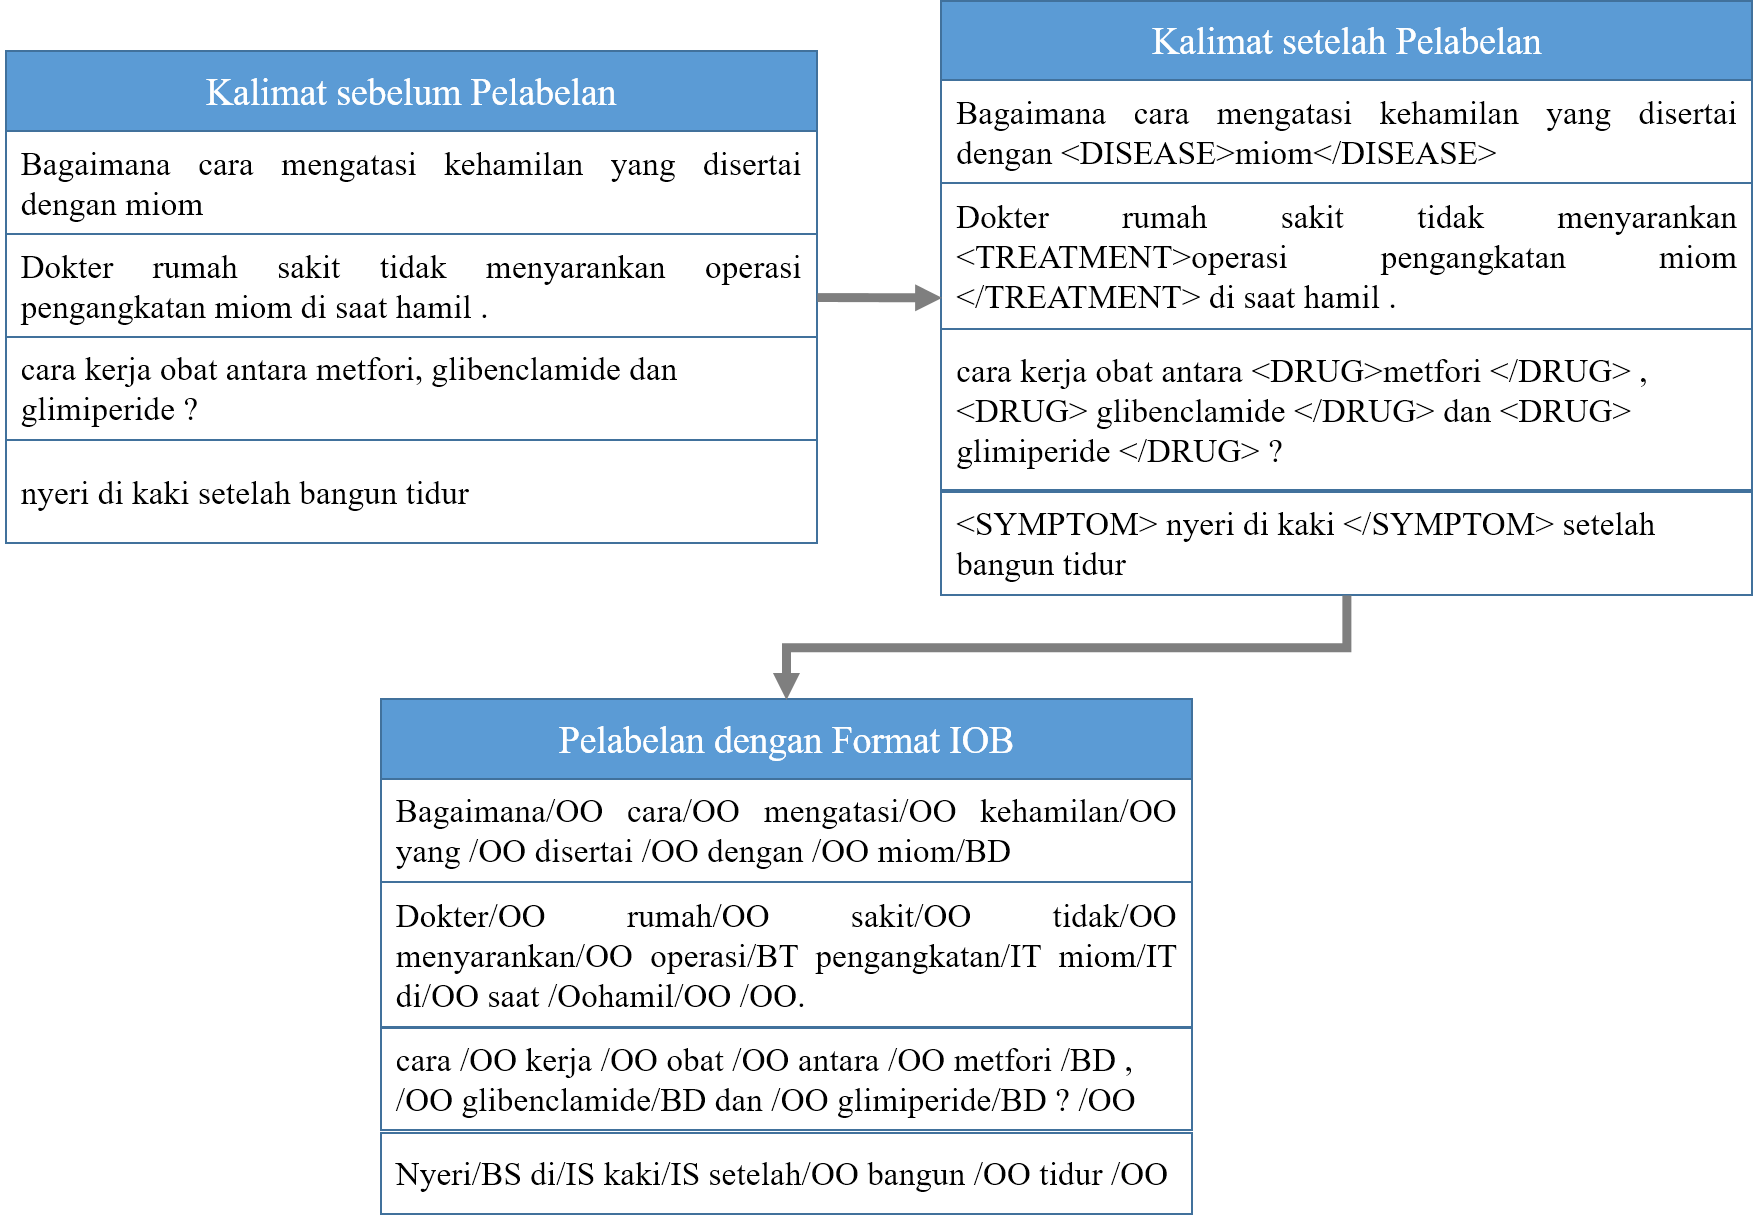
\includegraphics[width=\linewidth]{images/pelabelan}
	\caption{Ilustrasi Pelabelan Entitas pada suatu Kalimat}
	\label{fig:pelabelan}
\end{figure}

Setelah pelabelan selesai dilakukan, supaya model RNNs mampu mengenali masing-masing label, \saya~menggunakan \textit{one-hot-vector} untuk merepresentasikan masing-masing label. Tabel \ref{table:onehotlabel} merupakan tabel pemetaan dari label menjadi represebtasinya dalam \textit{one-hot-vector}.

\begin{table}
	\centering
	\caption{Tabel Pemetaan Label dengan Representasi \textit{One-Hot-Vector}}
	\label{table:onehotlabel}
	\begin{tabular}{|l|l|}
		\hline
		\multicolumn{1}{|c|}{Label IOB} & \multicolumn{1}{c|}{\textit{One-hot-vector}} \\ \hline
		BD & {[} 0, 0, 0, 0, 0, 0, 0, 0, 1 {]} \\ \hline
		ID & {[} 0, 0, 0, 0, 0, 0, 0, 1, 0 {]} \\ \hline
		BS & {[} 0, 0, 0, 0, 0, 0, 1, 0, 0 {]} \\ \hline
		IS & {[} 0, 0, 0, 0, 0, 1, 0, 0, 0 {]} \\ \hline
		BT & {[} 0, 0, 0, 0, 1, 0, 0, 0, 0 {]} \\ \hline
		IT & {[} 0, 0, 0, 1, 0, 0, 0, 0, 0 {]} \\ \hline
		BG & {[} 0, 0, 1, 0, 0, 0, 0, 0, 0 {]} \\ \hline
		IG & {[} 0, 1, 0, 0, 0, 0, 0, 0, 0 {]} \\ \hline
		OO & {[} 1, 0, 0, 0, 0, 0, 0, 0, 0 {]} \\ \hline
	\end{tabular}
\end{table}

Gambar \ref{fig:labeltoone} merupakan contoh pengubahan kata menjadi \textit{one-hot-vector} dalam suatu kalimat.

\begin{figure}
	\centering
	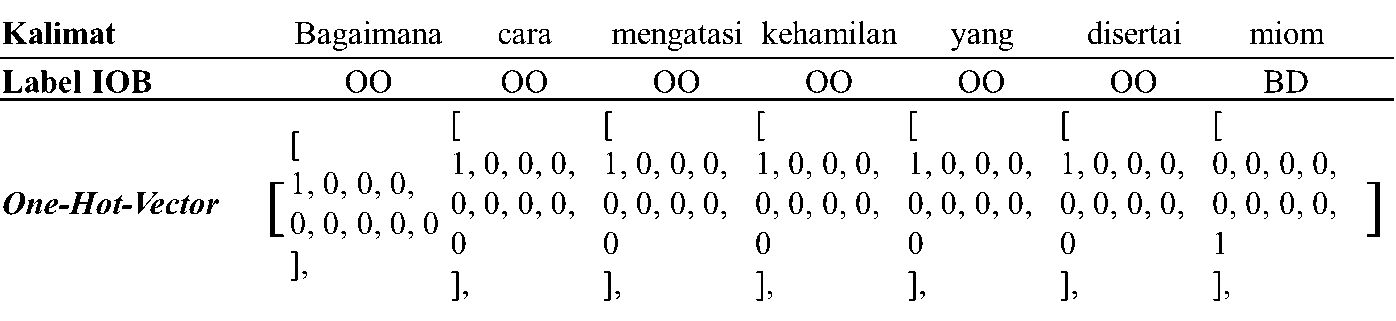
\includegraphics[width=\linewidth]{images/labeltoone}
	\caption{Ilustrasi Pengubahan Label menjadi \textit{One-Hot-Vector}}
	\label{fig:labeltoone}
\end{figure}

\section{Pengembangan Model}
Pada tahap ini, \saya~melakukan pengusulan dan perancangan model yang nantinya akan \saya~evaluasi pada tahap eksperimen. Dalam mengembangkan model, terdapat dua pekerjaan yang \saya~lakukan, yaitu:

\subsection{Ekstrasi Fitur}\label{subbab:fitur}
Pada tahap ini, \saya~melakukan ekstraksi fitur dari dokumen yang telah diberi label entitas. Ada beberapa fitur yang \saya~usulkan dalam penelitian ini yang nantinya \saya~kombinasikan supaya mendapatkan hasil terbaik. Fitur-fitur tersebut yaitu:
\begin{enumerate}
	\item Fitur 1: Kata itu sendiri\\
	Fitur ini merupakan fitur kata dalam representasi vektor. Fitur ini merupakan fitur yang digunakan \cite{abacha2011medical} dan \cite{skripsiKakRadit} dalam penelitian tentang \mer. Untuk mendapatkan representasi vektor dari masing-masing kata, penulis menggunakan \textit{word embedding}. Pada penelitian mengenai \mer~yang dilakukan oleh \cite{mujiono2016new}, hasil dari representasi data terbaik yaitu \textit{word embedding}. Selain itu, seperti yang dijelaskan pada Bab 2, \textit{word embedding} memberikan hasil yang sangat baik dalam bidang NLP. Oleh karena itu, \saya~menggunakan \textit{word embedding} untuk mendapatkan representasi vektor masing-masing kata. Dalam penelitian ini. Terdapat beberapa langkah yang perlu \saya~lakukan dalam memanfaatkan \textit{word embedding} ini, yaitu:
	\begin{enumerate}
		\item Pengumpulan data \textit{training} untuk \textit{word embedding}\\
		\Saya~melakukan pengumpulan data teks sebagai \textit{resource} untuk melakukan \textit{training} model \textit{word embedding}. Data teks yang \saya~gunakan merupakan data teks dari artikel-artikel kesehatan dan data teks forum kesehatan di kaskus. \Saya~menggunakan teks berjenis kesehatan supaya \textit{domain word embedding} dengan data \textit{training} untuk model \mer~sama. Selain itu, terdapat beberapa \textit{term} kesehatan yang susah ditemukan di forum umum.
		 
		\item \textit{Training} untuk mendapatkan model \textit{word embedding}\\
		\textit{Training} dilakukan untuk mendapatkan model yang mampu mendapatkan representasi vektor dari sebuah kata. Panjang vektor yang dihasilkan yaitu 128 dengan besaran \textit{window} yaitu 5. Arsitektur yang digunakan untuk melakukan \textit{training} ini adalah \textit{skip-gram}.
		
		\item Pengubahan kata menjadi vektor dari model yang didapatkan\\
		Pada langkah ini \saya~mengubah masing-masing kata dalam kalimat menjadi representasi vektor dengan model yang telah \saya~dapatkan pada tahap \textit{training} model \textit{word embedding}.
	\end{enumerate}
	
	Gambar \ref{fig:fiturkata} merupakan ilustrasi dari proses ekstraksi fitur kata itu sendiri dalam suatu kalimat dengan menggunakan \textit{Word Embedding}.
	
	\begin{figure}
		\centering
		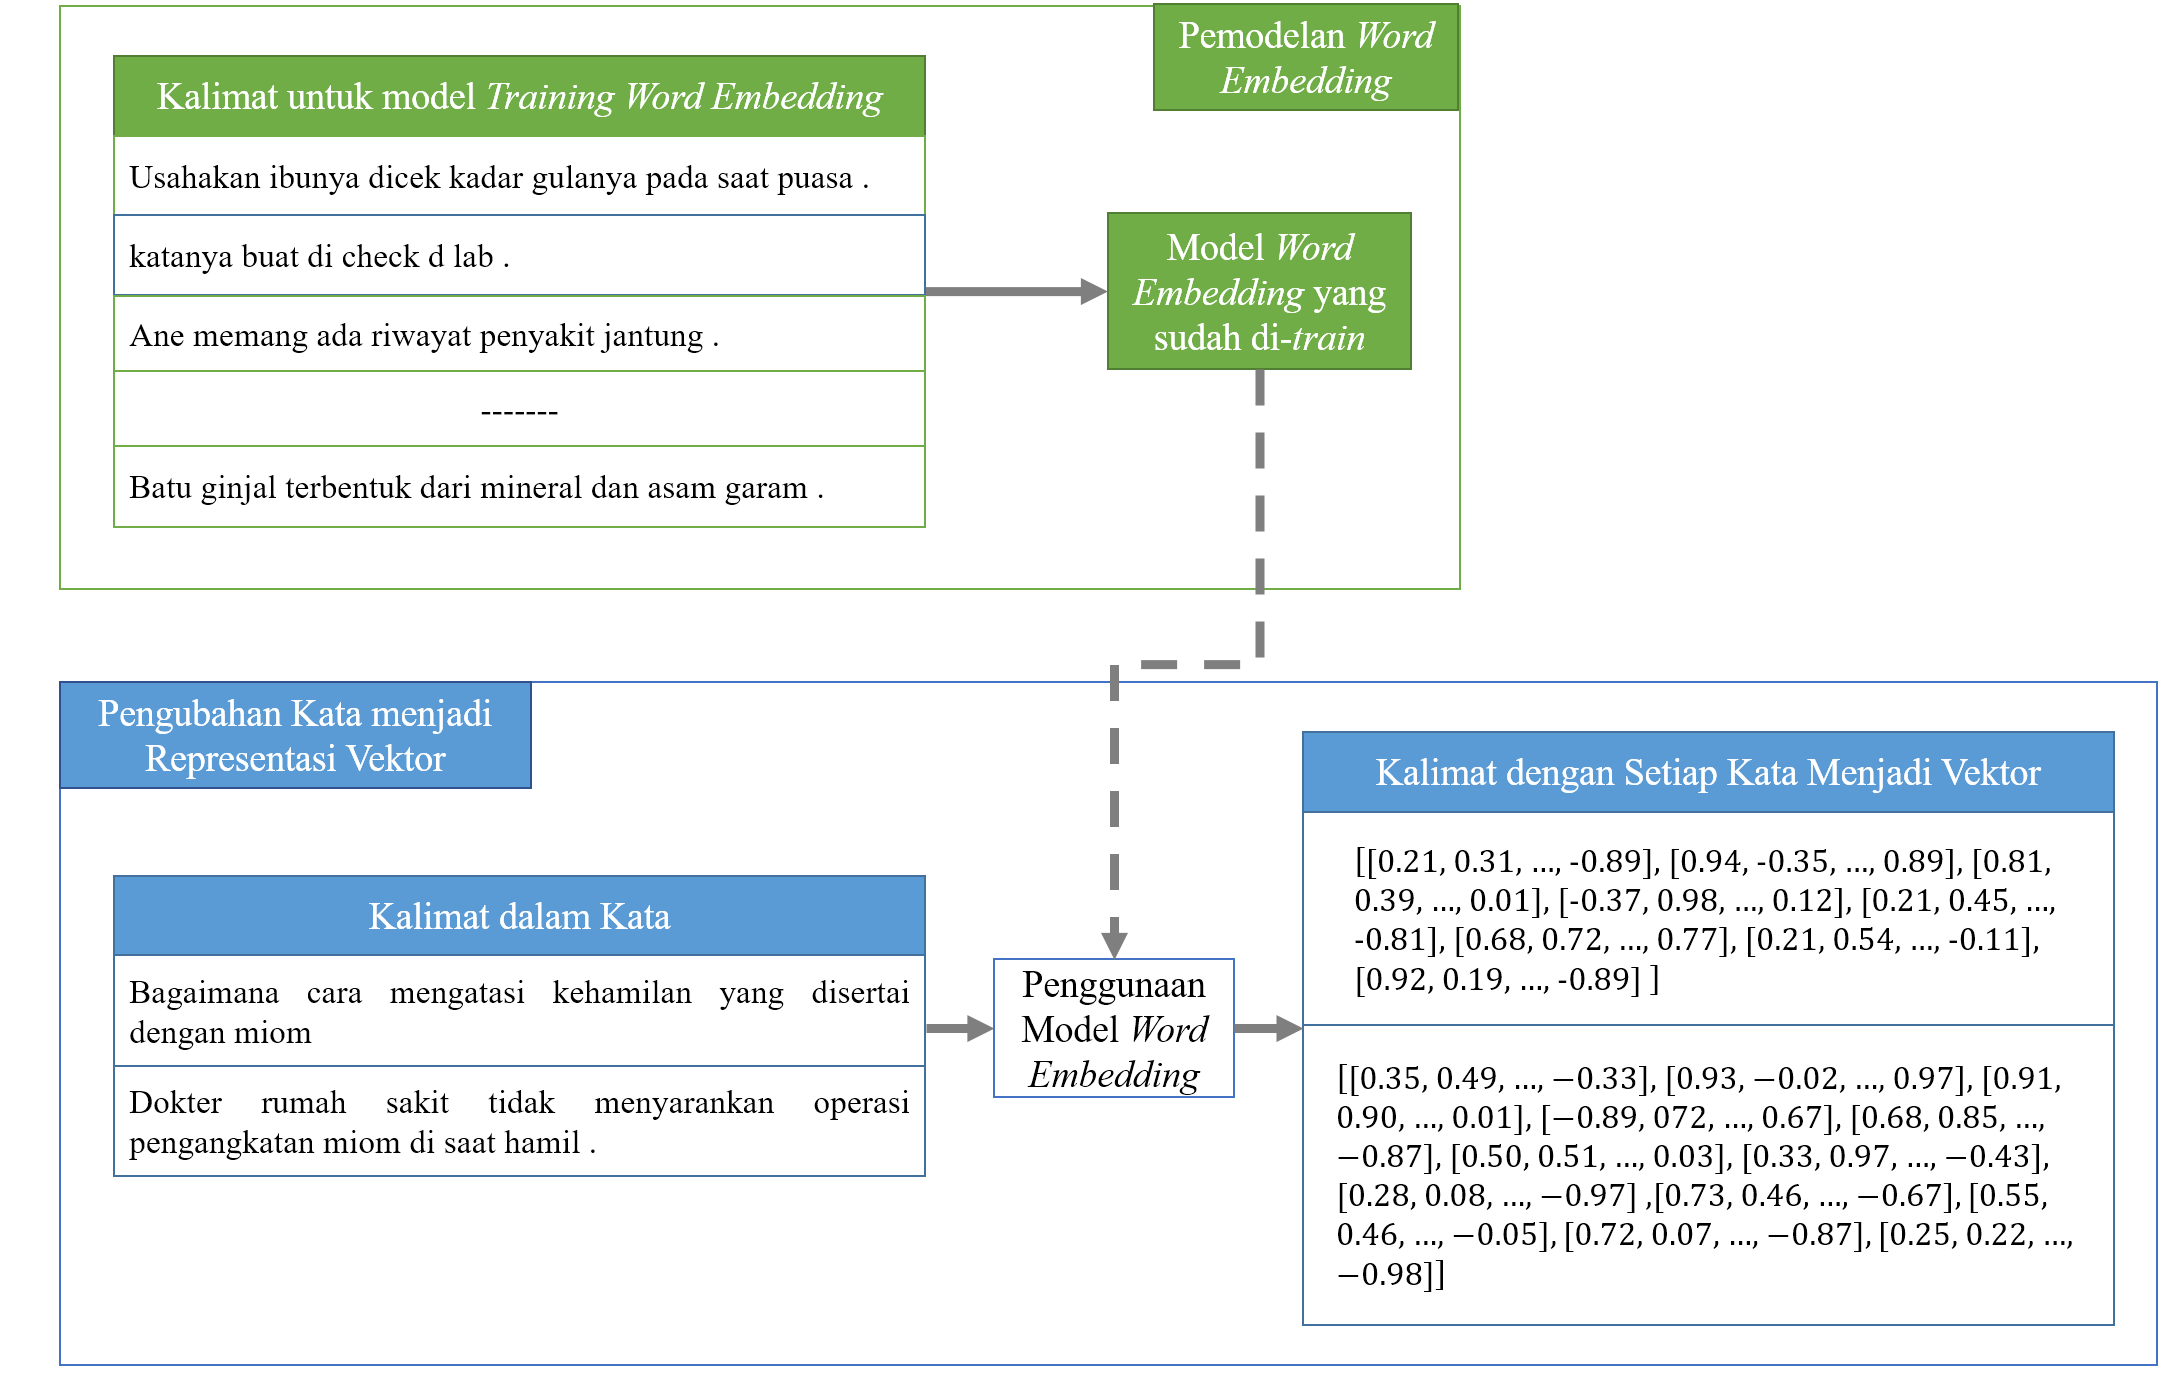
\includegraphics[width=\linewidth]{images/fiturkata}
		\caption{Ilustrasi Ekstraksi Fitur Kata pada Suatu Kalimat}
		\label{fig:fiturkata}
	\end{figure}
	
	\item Fitur 2: Kamus Kesehatan\\
	Fitur kamus kesehatan merupakan fitur yang berisi informasi suatu kata terdapat di dalam kamus kesehatan atau tidak. Fitur ini digunakan dalam penelitian \cite{skripsiKakRadit} dan memberikan kontribusi dalam hasil terbaik. Pada penelitian ini, kamus kesehatan yang dipakai merupakan kamus \disease, kamus \symptom, kamus \drug~dan kamus \treatment. Dengan menggunakan fitur ini diharapkan mampu berkontribusi dalam meningkatkan akurasi karena model akan mempertimbangkan apakah suatu kata termasuk di dalam kamus atau tidak. Gambar \ref{fig:fiturkamus} merupakan ilustrasi dari ekstraksi fitur kamus kesehatan dalam suatu kalimat.
	
	\begin{figure}
		\centering
		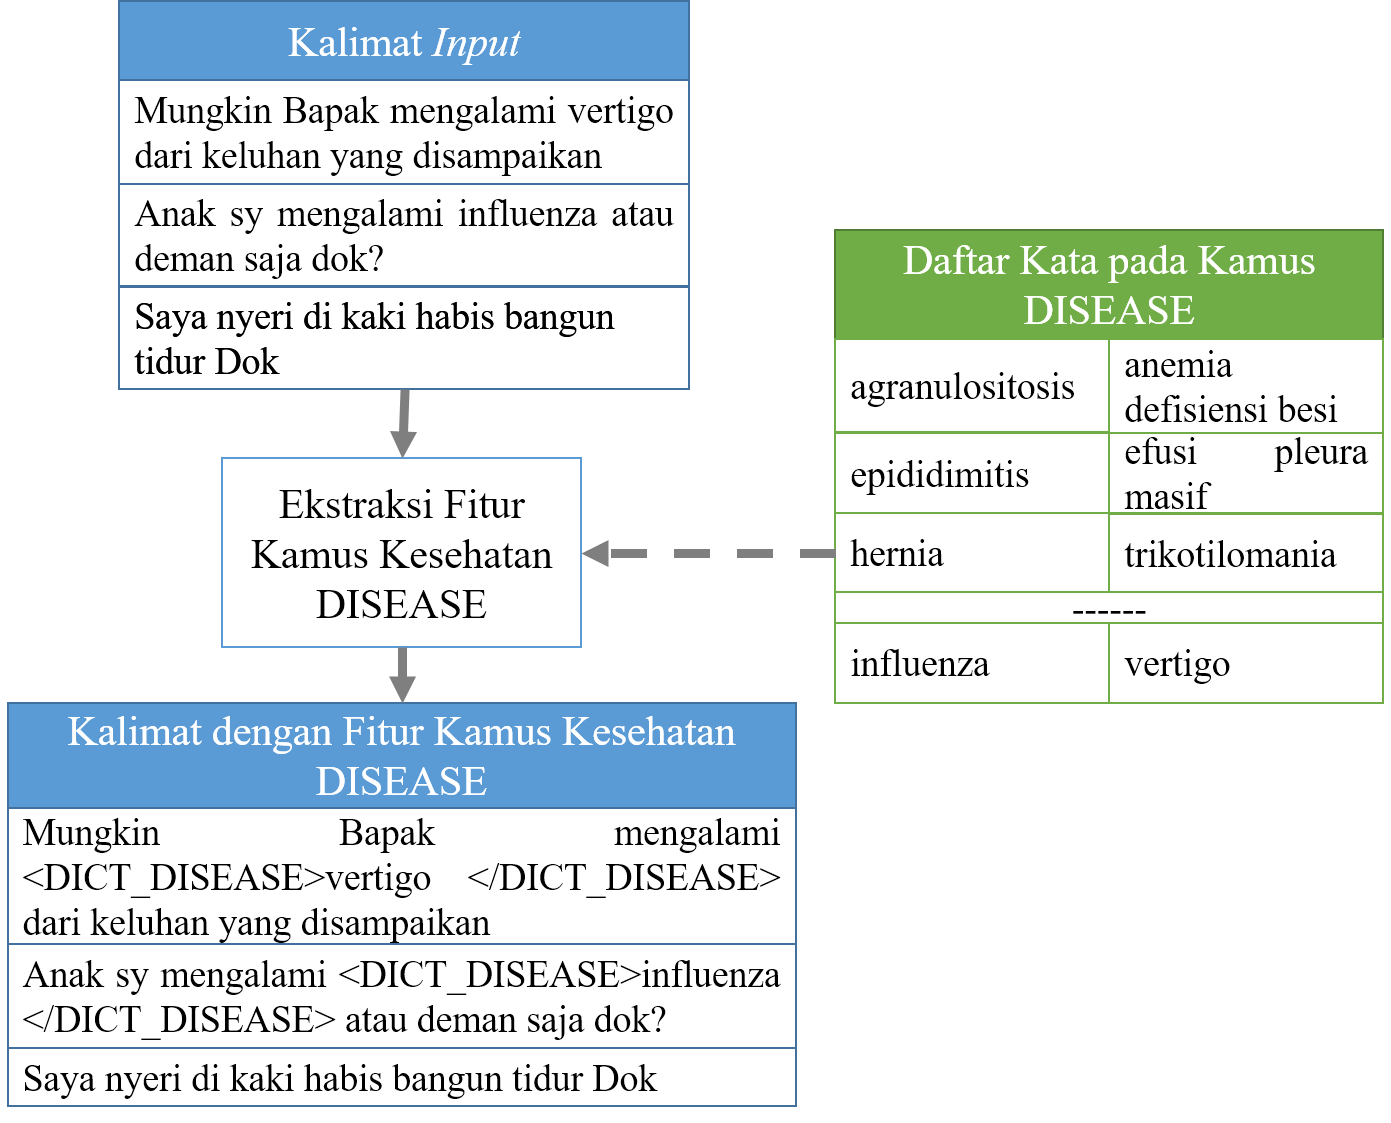
\includegraphics[width=\linewidth]{images/fiturkamus}
		\caption{Ilustrasi Ekstraksi Fitur Kamus \disease~pada Suatu Kalimat}
		\label{fig:fiturkamus}
	\end{figure}

	Supaya model RNNs mengenali fitur ini, \saya~menggunakan representasi \textit{one-hot vector}. Untuk suatu kata yang terdapat dalam kamus kesehatan, representasi vektornya adalah $ [0, 1] $, sedangkan yang tidak terdapat di dalam kamus kesehatan, representasi vektornya adalah $ [1, 0] $. Gambar \ref{fig:kamustoone} merupakan contoh pengubahan fitur kamus kesehatan menjadi representasi \textit{one-hot-vector}.
	
	\begin{figure}
		\centering
		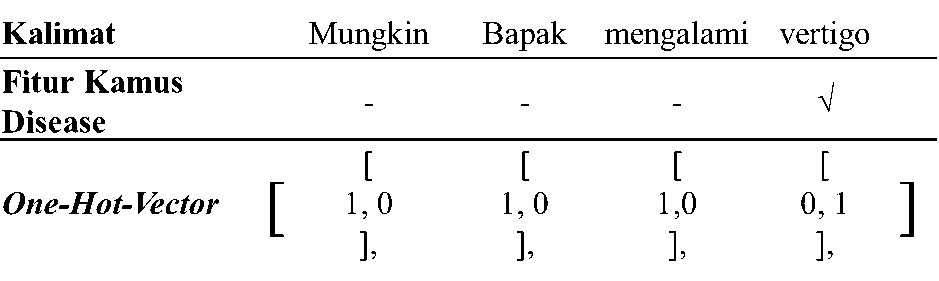
\includegraphics[width=0.85\linewidth]{images/kamustoone}
		\caption{Ilustrasi Pengubahan Label menjadi \textit{One-Hot-Vector}}
		\label{fig:kamustoone}
	\end{figure}
	
	\item Fitur 3: \textit{Stopword}\\
	Fitur ini merupakan fitur yang berisi vektor suatu kata merupakan \textit{stopword} atau bukan. Fitur ini \saya~gunakan dalam penelitian ini untuk membantu sistem dalam menghindari kesalahan pelabelan suatu kata yang bukan entitas namun dilabeli sebagai entitas.
	
	Ketika melakukan eksperimen, hasil yang \saya~dapatkan ternyata lebih bagus apabila mempertahankan fitur ini, oleh karena itu, \saya~mengusulkan untuk menggunakan fitur ini. Untuk pembahasan lebih lanjut dibahas pada Bab 5. Gambar \ref{fig:fiturstopword} merupakan ilustrasi dari ekstraksi fitur \textit{stopword} dalam suatu kalimat.
	
	\begin{figure}
		\centering
		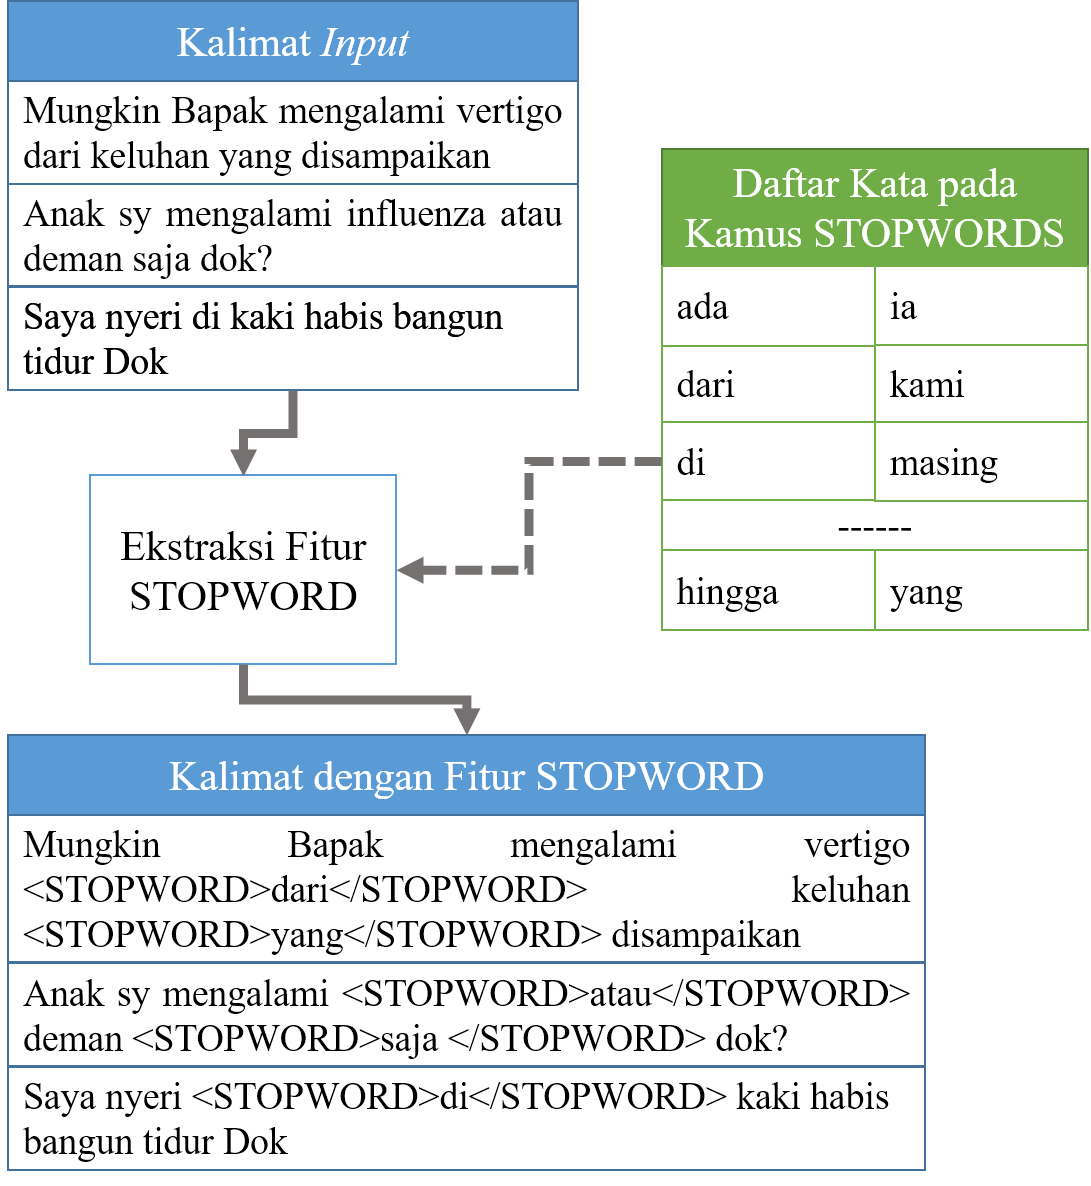
\includegraphics[width=\linewidth]{images/fiturstopword}
		\caption{Ilustrasi Ekstraksi Fitur \textit{Stopword} pada Suatu Kalimat}
		\label{fig:fiturstopword}
	\end{figure}

	Supaya model RNNs mengenali fitur ini, \saya~menggunakan representasi \textit{one-hot vector}. Untuk suatu kata yang merupakan \textit{stopword}, representasi vektornya adalah $ [0, 1] $, sedangkan yang bukan merupakan \textit{stopword}, representasi vektornya adalah $ [1, 0] $. Gambar \ref{fig:stopwordtoone} merupakan contoh pengubahan fitur \textit{stopword} menjadi representasi \textit{one-hot-vector}.
	
	\begin{figure}
		\centering
		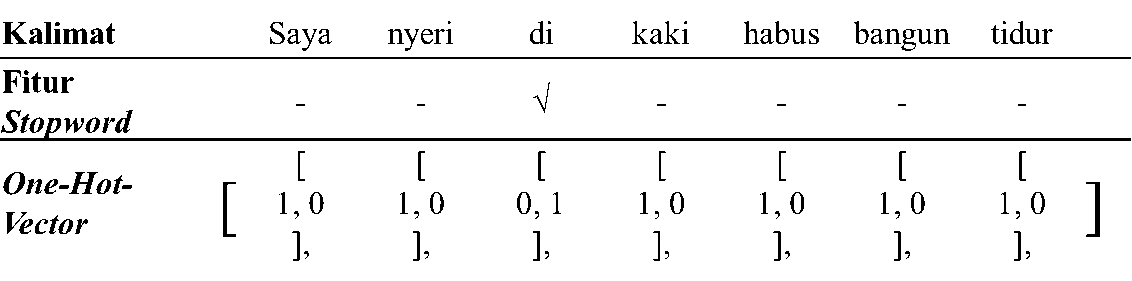
\includegraphics[width=0.85\linewidth]{images/stopwordtoone}
		\caption{Ilustrasi Pengubahan Label menjadi \textit{One-Hot-Vector}}
		\label{fig:stopwordtoone}
	\end{figure}

	\item Fitur 4: \textit{Part of Speech Tag} (POS-Tag)\\
	Fitur ini merupakan fitur \textit{tag} yang dimiliki setiap kata yang diusulkan oleh \cite{abacha2011medical} dalam penelitiannya di bidang \mer. Entitas-entitas tertentu memiliki tag yang sama, misalnya entitas obat dan penyakit pada umumnya memiliki tag "NNP" sehingga dengan digunakannya fitur ini sistem dapat mengenali jenis obat dan penyakit dengan lebih baik. Model POS-Tagger yang \saya~gunakan merupakan model POS-Tag berbahasa Indonesia. Gambar \ref{fig:fiturpostag} merupakan ilustrasi dari ekstraksi fitur POS-\textit{Tag} dalam suatu kalimat.
	
	\begin{figure}
		\centering
		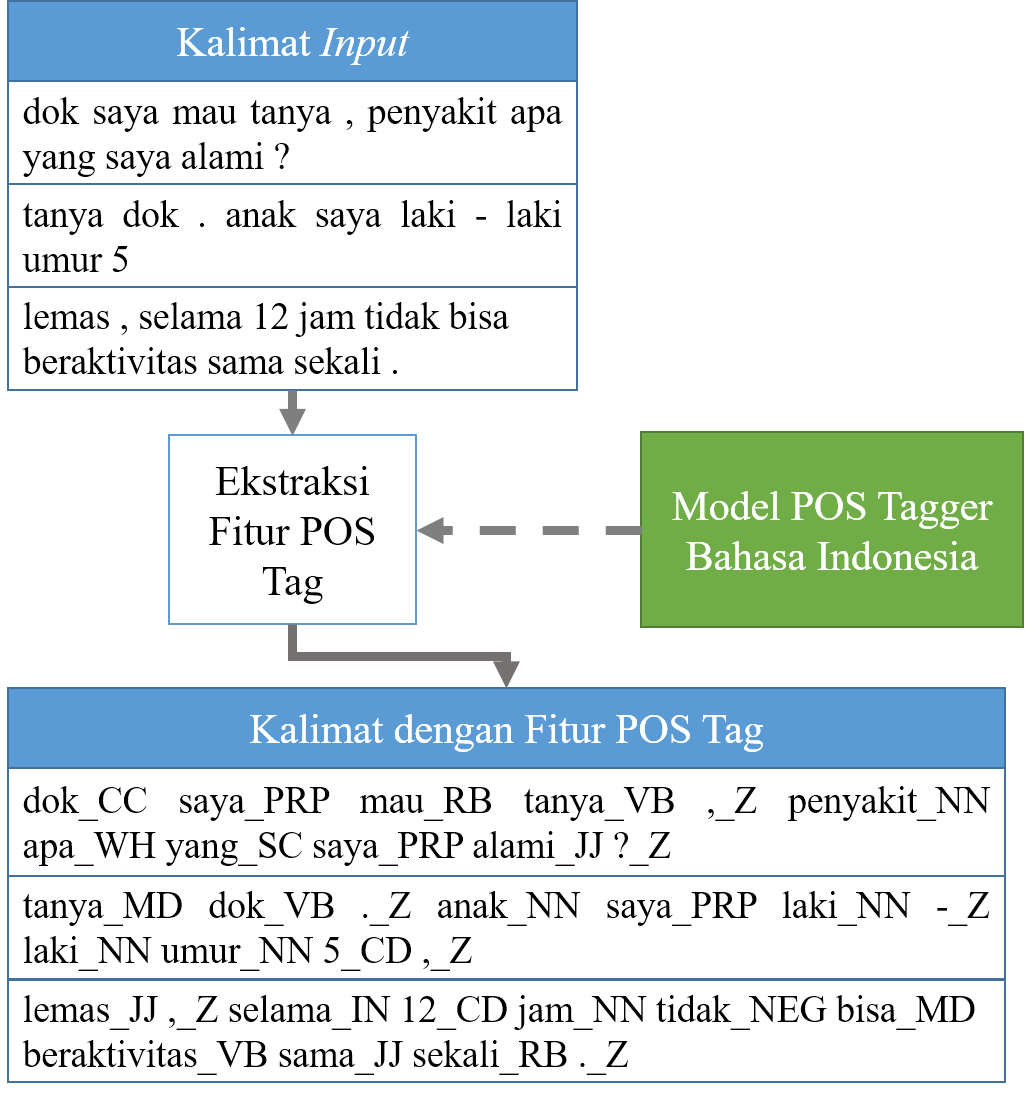
\includegraphics[width=\linewidth]{images/fiturpostag}
		\caption{Ilustrasi Ekstraksi Fitur POS \textit{Tag} pada Suatu Kalimat}
		\label{fig:fiturpostag}
	\end{figure}

	Setelah POS-Tag didapatkan, supaya model RNNs mampu mengenali masing-masing tag, \saya~menggunakan \textit{one-hot-vector} untuk merepresentasikan masing-masing label. Tabel \ref{table:onehotpostag} merupakan tabel pemetaan dari label menjadi representasinya dalam \textit{one-hot-vector}.
	
	\begin{table}
		\centering
		\caption{Tabel Pemetaan POS-Tag dengan Representasi \textit{One-Hot-Vector}}
		\label{table:onehotpostag}
		\begin{tabular}{|l|l|}
			\hline
			\multicolumn{1}{|c|}{Label POS-Tag} & \multicolumn{1}{c|}{\textit{One-hot-vector}} \\ \hline
			JJ & {[}0,0,0,0,0,0,0,0,0,0,0,0,0,0,0,0,0,0,0,0,0,0,0,1{]} \\ \hline
			NN & {[}0,0,0,0,0,0,0,0,0,0,0,0,0,0,0,0,0,0,0,0,0,0,1,0{]} \\ \hline
			NNP & {[}0,0,0,0,0,0,0,0,0,0,0,0,0,0,0,0,0,0,0,0,0,1,0,0{]} \\ \hline
			Z & {[}0,0,0,0,0,0,0,0,0,0,0,0,0,0,0,0,0,0,0,0,1,0,0,0{]} \\ \hline
			IN & {[}0,0,0,0,0,0,0,0,0,0,0,0,0,0,0,0,0,0,0,1,0,0,0,0{]} \\ \hline
			PRP & {[}0,0,0,0,0,0,0,0,0,0,0,0,0,0,0,0,0,0,1,0,0,0,0,0{]} \\ \hline
			MD & {[}0,0,0,0,0,0,0,0,0,0,0,0,0,0,0,0,0,1,0,0,0,0,0,0{]} \\ \hline
			VB & {[}0,0,0,0,0,0,0,0,0,0,0,0,0,0,0,0,1,0,0,0,0,0,0,0{]} \\ \hline
			SC & {[}0,0,0,0,0,0,0,0,0,0,0,0,0,0,0,1,0,0,0,0,0,0,0,0{]} \\ \hline
			RB & {[}0,0,0,0,0,0,0,0,0,0,0,0,0,0,1,0,0,0,0,0,0,0,0,0{]} \\ \hline
			CC & {[}0,0,0,0,0,0,0,0,0,0,0,0,0,1,0,0,0,0,0,0,0,0,0,0{]} \\ \hline
			NEG & {[}0,0,0,0,0,0,0,0,0,0,0,0,1,0,0,0,0,0,0,0,0,0,0,0{]} \\ \hline
			WH & {[}0,0,0,0,0,0,0,0,0,0,0,1,0,0,0,0,0,0,0,0,0,0,0,0{]} \\ \hline
			CD & {[}0,0,0,0,0,0,0,0,0,0,1,0,0,0,0,0,0,0,0,0,0,0,0,0{]} \\ \hline
			X & {[}0,0,0,0,0,0,0,0,0,1,0,0,0,0,0,0,0,0,0,0,0,0,0,0{]} \\ \hline
			PR & {[}0,0,0,0,0,0,0,0,1,0,0,0,0,0,0,0,0,0,0,0,0,0,0,0{]} \\ \hline
			RP & {[}0,0,0,0,0,0,0,1,0,0,0,0,0,0,0,0,0,0,0,0,0,0,0,0{]} \\ \hline
			FW & {[}0,0,0,0,0,0,1,0,0,0,0,0,0,0,0,0,0,0,0,0,0,0,0,0{]} \\ \hline
			NND & {[}0,0,0,0,0,1,0,0,0,0,0,0,0,0,0,0,0,0,0,0,0,0,0,0{]} \\ \hline
			DT & {[}0,0,0,0,1,0,0,0,0,0,0,0,0,0,0,0,0,0,0,0,0,0,0,0{]} \\ \hline
			OD & {[}0,0,0,1,0,0,0,0,0,0,0,0,0,0,0,0,0,0,0,0,0,0,0,0{]} \\ \hline
			UH & {[}0,0,1,0,0,0,0,0,0,0,0,0,0,0,0,0,0,0,0,0,0,0,0,0{]} \\ \hline
			SYM & {[}0,1,0,0,0,0,0,0,0,0,0,0,0,0,0,0,0,0,0,0,0,0,0,0{]} \\ \hline
			fw & {[}1,0,0,0,0,0,0,0,0,0,0,0,0,0,0,0,0,0,0,0,0,0,0,0{]} \\ \hline
		\end{tabular}
	\end{table}

	Gambar \ref{fig:postagtoone} merupakan contoh pengubahan fitur POS-Tag menjadi \textit{one-hot-vector} dalam suatu kalimat.
	
	\begin{figure}
		\centering
		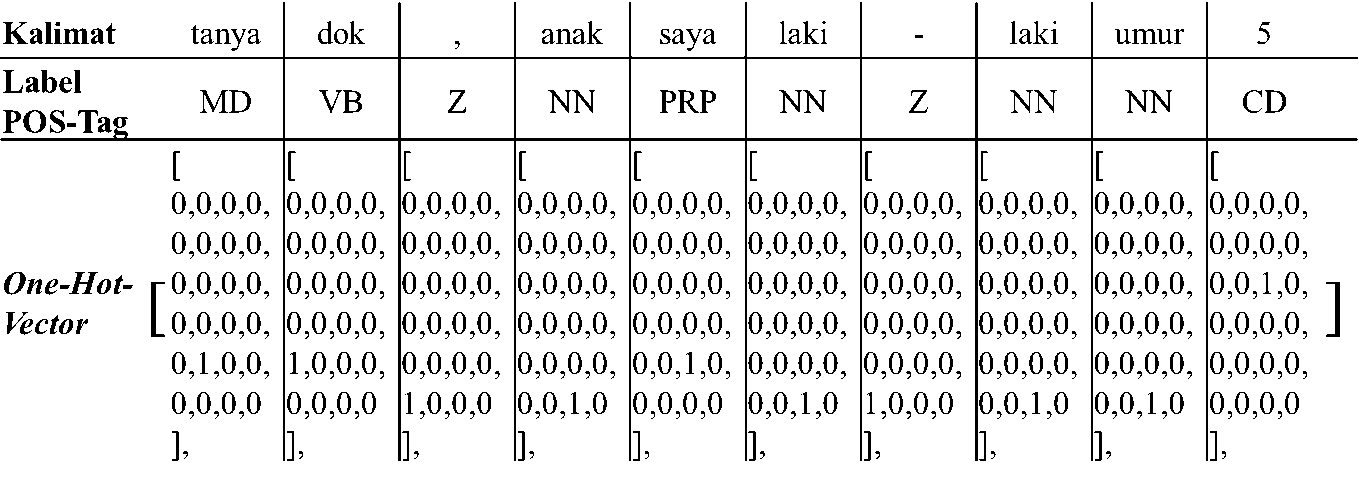
\includegraphics[width=\linewidth]{images/postagtoone}
		\caption{Ilustrasi Pengubahan Fitur POS-Tag menjadi \textit{One-Hot-Vector}}
		\label{fig:postagtoone}
	\end{figure}
		
	\item Fitur 5: Frasa Kata\\
	Pada penelitian ini, \saya~mengusulkan fitur frasa kata karena entitas \textit{symptom} dan \textit{treatment}  pada umumnya merupakan frasa kata kerja. Sedangkan entitas \textit{disease} dan \textit{drug} pada umumnya entitas yang akan dikenali pada penelitian ini merupakan frasa kata benda. Selain itu, pada penelitian \cite{skripsiKakRadit}, fitur ini berkontribusi dalam memberikan hasil terbaik. Oleh karena itu, \saya~berharap bahwa dengan diusulkannya fitur ini akan mampu menambah akurasi dari model yang diusulkan.
	
	Pada penelitian ini ada dua frasa yang diujicobakan, yaitu:
	\begin{enumerate}
		\item Frasa Kata Benda (Nomina)
		Menurut \cite{hs2005bahasa}, frasa kata benda sendiri merupakan kelompok kata benda yang dibentuk dengan memperluas kata benda ke sekelilingnya. Fitur frasa kata benda yang \saya~gunakan dalam penelitian merupakan fitur yang berisi informasi suatu kata atau kumpulan kata merupakan frasa kata benda atau bukan. Dalam menentukan suatu kata merupakan frasa atau bukan, penulis menggunakan aturan pembentukan frasa yang digunakan pada bahasa Indonesia, yaitu:
		\begin{description}
			\item[$\bullet$] NP : NN
			\item[$\bullet$] NP : NNP
			\item[$\bullet$] NP : PR
			\item[$\bullet$] NP : PRP
			\item[$\bullet$] NP : NN + NN
			\item[$\bullet$] NP : NN + NNP
			\item[$\bullet$] NP : NN + PR
			\item[$\bullet$] NP : NN + PRP
			\item[$\bullet$] NP : NN + JJ
			\item[$\bullet$] NP : DT + NN
			\item[$\bullet$] NP : RB + NN
			\item[$\bullet$] NP : CD + NN
			\item[$\bullet$] NP : NND + NN
		\end{description}
		
		\item Frasa Kata Kerja (Verbal)\\
		Menurut \cite{hs2005bahasa}, frasa verbal merupakan kelompok kata benda yang dibentuk dengan kata kerja. Fitur frasa verbal yang \saya~gunakan dalam penelitian merupakan fitur yang berisi informasi suatu kata atau kumpulan kata merupakan frasa verbal atau bukan. Dalam menentukan suatu kata merupakan frasa atau bukan, penulis menggunakan aturan pembentukan frasa yang digunakan pada bahasa Indonesia, yaitu:
		\begin{description}
			\item[$\bullet$] VP : VB
			\item[$\bullet$] VP : VB + NP
		\end{description}
	\end{enumerate}

Gambar \ref{fig:fiturfrasa} merupakan ilustrasi dari ekstraksi fitur Frasa Nomina dalam suatu kalimat.

\begin{figure}
	\centering
	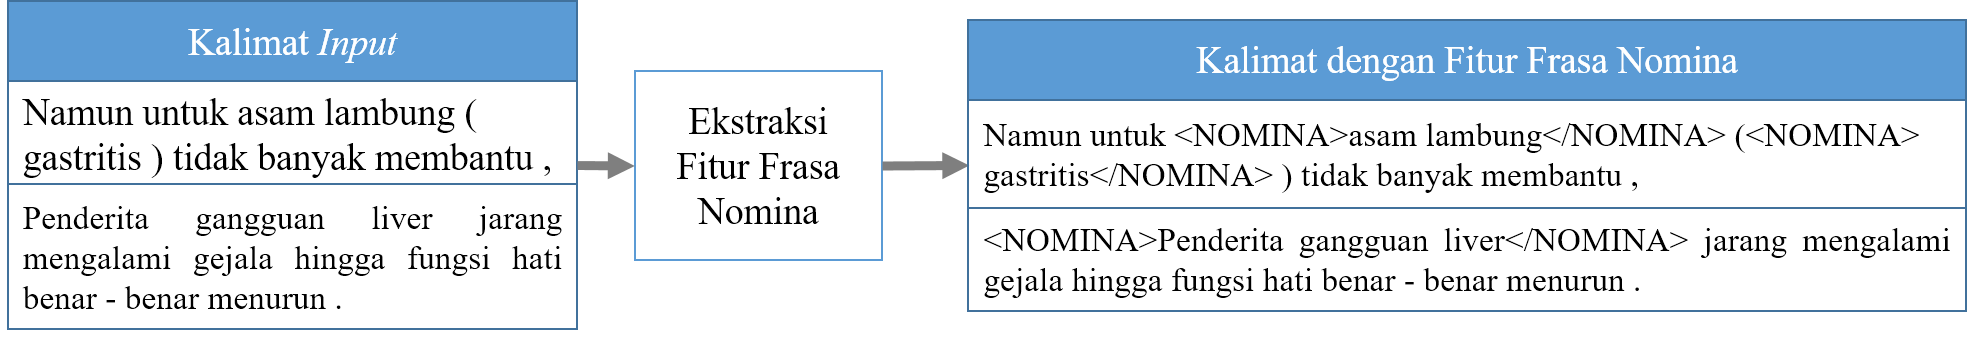
\includegraphics[width=\linewidth]{images/fiturfrasa}
	\caption{Ilustrasi Ekstraksi Fitur Frasa Nomina pada Suatu Kalimat}
	\label{fig:fiturfrasa}
\end{figure}

Supaya model RNNs mengenali fitur ini, \saya~menggunakan representasi \textit{one-hot vector}. Untuk suatu kata yang merupakan sebuah frasa, representasi vektornya adalah $ [0, 1] $, sedangkan yang bukan, representasi vektornya adalah $ [1, 0] $. Gambar \ref{fig:frasatoone} merupakan contoh pengubahan fitur frasa nomina menjadi representasi \textit{one-hot-vector}.

\begin{figure}
	\centering
	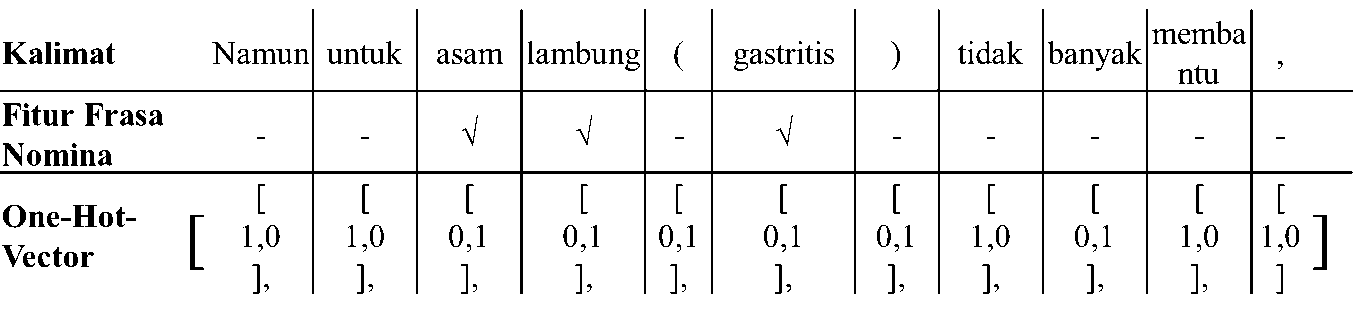
\includegraphics[width=0.85\linewidth]{images/frasatoone}
	\caption{Ilustrasi Pengubahan Fitur Frasa menjadi \textit{One-Hot-Vector}}
	\label{fig:frasatoone}
\end{figure}

 \item Fitur 6: 1 Kata Sebelum\\
 Fitur ini merupakan fitur yang berisi informasi kata sebelum kata saat ini yang direpresentasikan dalam bentuk vektor untuk masing-masing kata. Fitur ini digunakan pada penelitian penelitian \cite{skripsiKakRadit} yang juga berkontribusi memberikan hasil terbaik pada penelitiannya. Menurut \saya, ada beberapa entitas yang akan lebih mudah diketahui apabila diketahui kata sebelumnya. Misalnya kata "masuk angin", apabila hanya diberikan informasi kata "angin" tanpa kata "masuk", akan lebih sulit menentukan kata tersebut bagian dari suatu entitas \textit{disease} atau bukan.
  
 \item Fitur 7: 1 Kata Sesudah\\
 Fitur ini merupakan fitur yang berisi informasi kata sesudah kata saat ini yang direpresentasikan dalam bentuk vektor untuk masing-masing kata. Sama seperti pada fitur 1 Kata Sebelum, ada beberapa kasus yang mana apabila suatu kata merupakan sebuah entitas, akan lebih mudah dikenali apabila melihat kata atau konteks setelahnya. Sama seperti contoh pada Fitur 1 Kata Sebelum, misal diberikan kata "masuk angin", apabila hanya diberikan informasi "masuk" tanpa "angin", akan lebih sulit mengenali apakah kata tersebut termasuk entitas \textit{disease} atau bukan. Selain itu, fitur ini juga dapat membedakan kata berentitas dengan kata yang bukan, misalnya kata "masuk angin" dengan "masuk rumah". Apabila informasi pada saat tersebut hanya diberikan kata "masuk" saja tanpa kata setelahnya, akan lebih sulit mengenali kata tersebut termasuk kata berentitas atau bukan.
  
\end{enumerate}

\subsection{Pengusulan Arsitektur RNNs}
Pada tahap ini \saya~mengusulkan arsitektur RNNs yang akan digunakan pada tahap eksperimen. Ada dua arsitektur yang \saya~gunakan dalam penelitian ini, yaitu
\begin{enumerate}
	\item LSTMs 1 layer\\
	Pada LSTMs 1 layer, semua fitur yang menjadi input pada sebuah \textit{timestep} digabung menjadi satu. Untuk menentukan label, \saya~menggunakan \textit{feed-forward Neural Networks} pada masing-masing \textit{timestep} di layer terakhir. Berikut merupakan ilustrasi LSTM 1 layer yang \saya~gunakan dalam penelitian ini.
	
	\begin{figure}
		\centering
		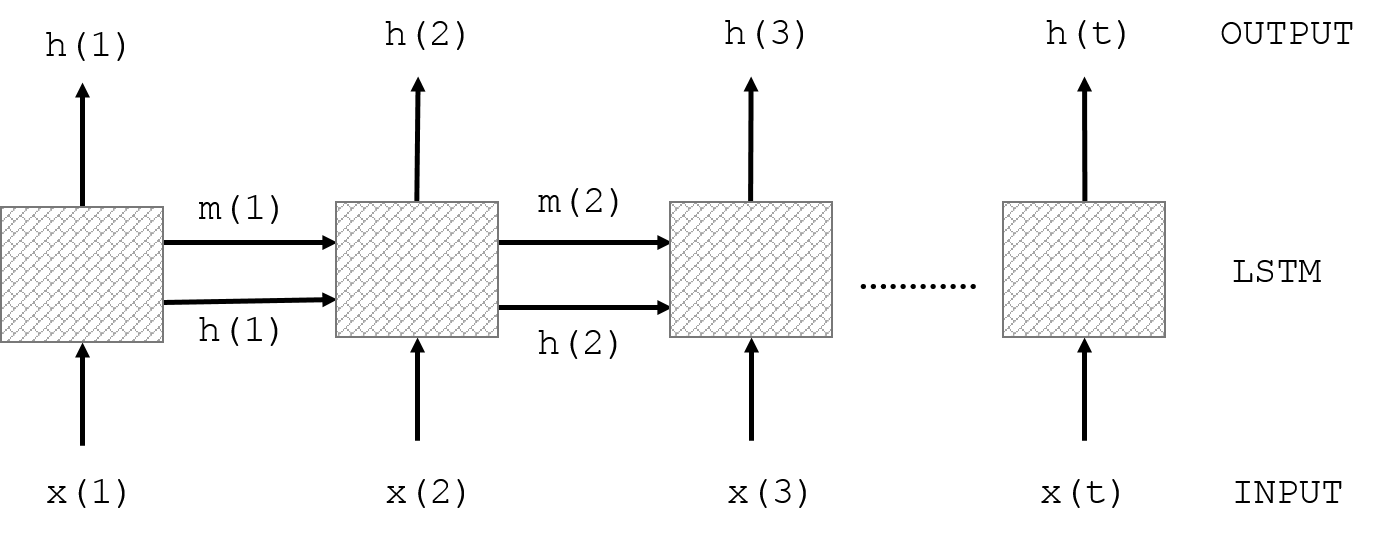
\includegraphics[width=0.8\linewidth]{images/lstm1}
		\caption{LSTMs 1 layer}
		\label{fig:single_layer_rnn}
	\end{figure}

	Misalnya fitur yang digunakan adalah fitur kata dan frasa. Karena hanya terdapat 1 layer saja, kedua fitur ini digabung terlebih dahulu menjadi 1. Gambar \ref{fig:inputlstm} merupakan ilustrasi dari proses penggabungan fitur supaya menjadi \textit{input} RNNs, dan  \textit{output} serta pemetaan menjadi label pada arsitektur ini.
	\begin{figure}
		\centering
		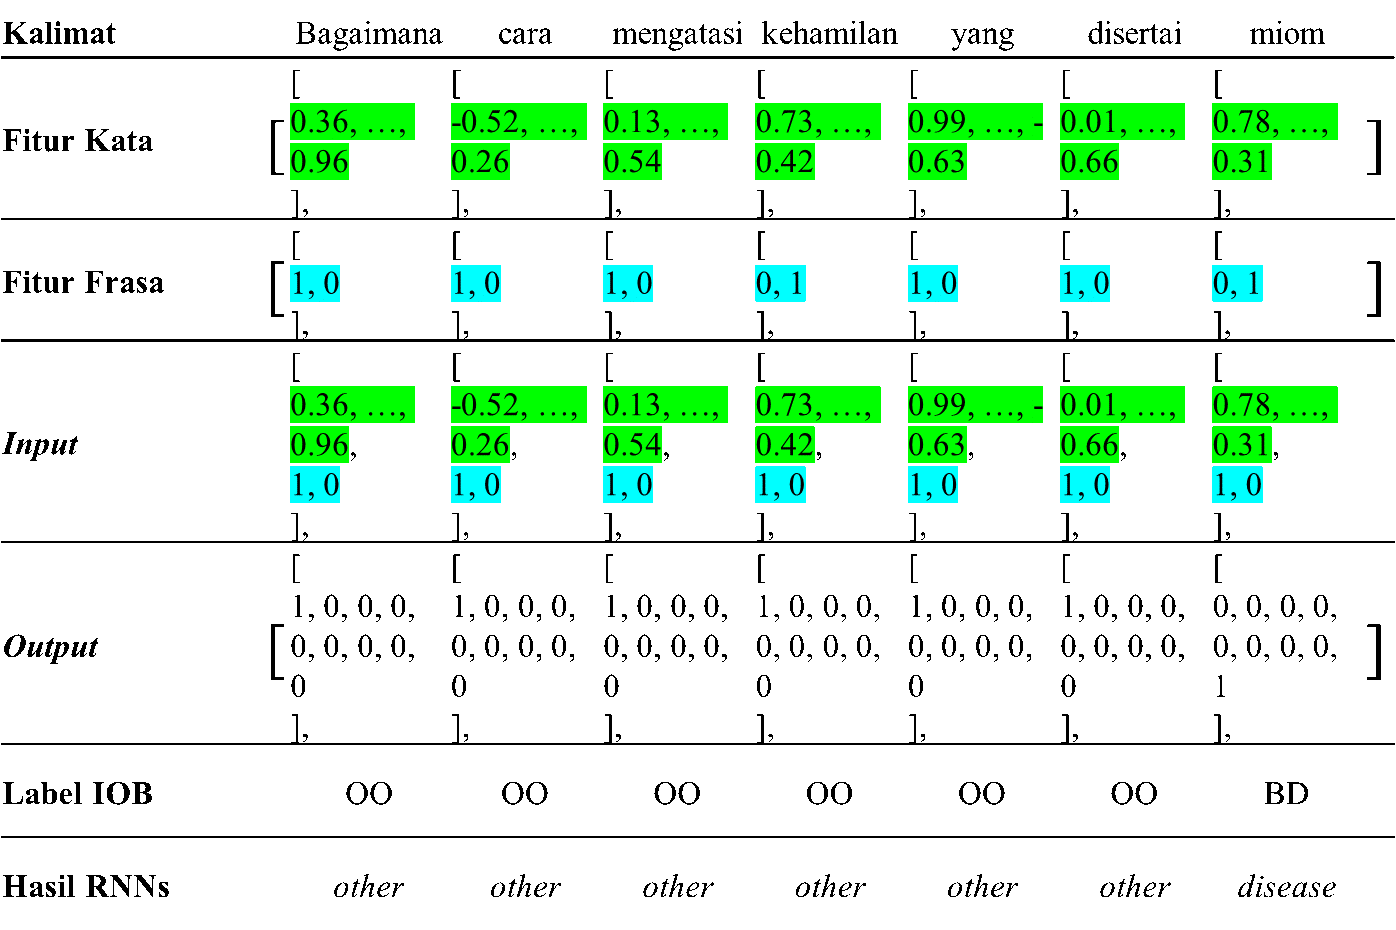
\includegraphics[width=0.85\linewidth]{images/concatlstm1}
		\caption{Ilustrasi penggabungan fitur kata dan frasa untuk menjadi \textit{input} LSTMs 1 layer dan \textit{output}-nya}
		\label{fig:inputlstm}
	\end{figure}
	
	Untuk masing-masing \textit{timestep} $ t $, berikut merupakan gambar sebuah \textit{cell}-nya.
	\begin{figure}
		\centering
		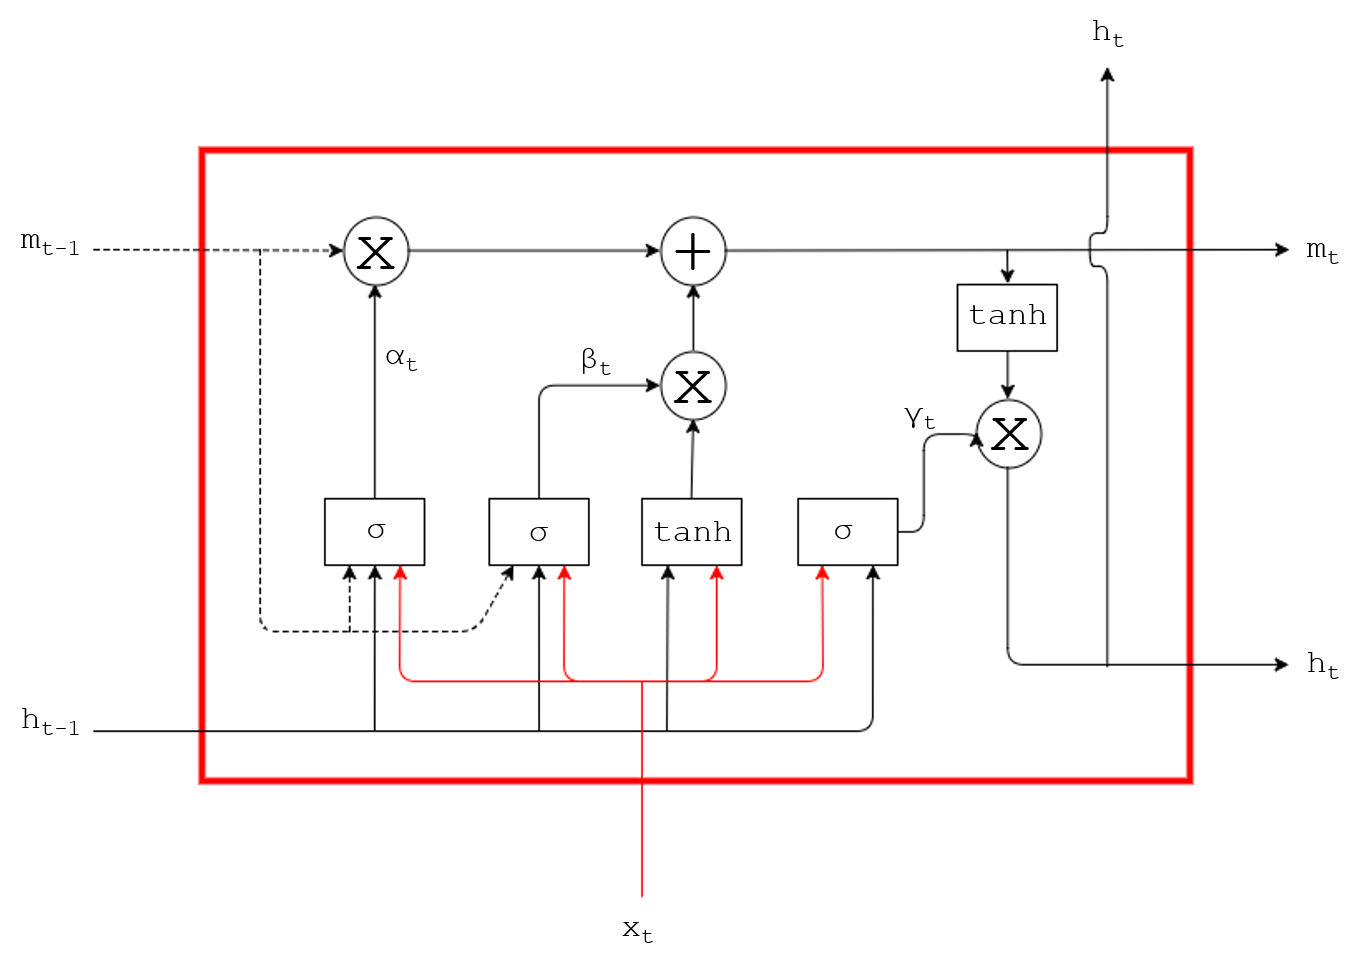
\includegraphics[width=0.85\linewidth]{images/lstm}
		\caption{1 buah blok memori dalam LSTM}
		\label{fig:lstm1cell}
	\end{figure}
	
	Dari gambar \ref{fig:lstm1cell}, sebuah \textit{cell} membutuhkan \textit{input} $ x(t) $ dan \textit{output} $ h(t) $. $ x(t) $ merupakan vektor dengan panjang $ N $, dan $ h(t) $ merupakan vektor dengan panjang $ M $. Seperti yang telah dijelaskan pada subbab \ref{subbab:lstm}, berikut merupakan formula untuk mengetahui \textit{output} pada \textit{timestep} $ t $.
	\begin{equation}\label{eq:lstmm}
	m_{t}=\alpha_{t} (\times) m_{t-1} + \beta_{t} (\times) f(x_{t},{t-1})
	\end{equation}
	\begin{equation}\label{eq:lstmh}
	h_{t}=\gamma_{t} (\times) tanh(m_{t})
	\end{equation}
	dimana
	\begin{equation}\label{eq:lstmx}
	f(x_{t},{t-1})=tanh(W_{xm} \cdot x_{t} + W_{hm} \cdot h_{t-1})
	\end{equation}
	
	$ \alpha_t $, $ \beta_t $ dan $ \gamma_t $ merupakan \textit{gates}:
	\begin{enumerate}
		\item \textit{Forget gates}: $ \alpha_{t}=\sigma(W_{x\alpha}+W_{h\alpha}\cdot~h_{t-1}+W_{m\alpha}\cdot~m_{t-1}) $
		\item \textit{Input gates}: $ \beta_{t}=\sigma(W_{x\beta}+W_{h\beta}\cdot~h_{t-1}+W_{m\beta}\cdot~m_{t-1}) $
		\item \textit{Output gates}: $ \gamma_{t}=\sigma(W_{x\gamma}+W_{h\gamma}\cdot~h_{t-1}+W_{m\gamma}\cdot~m_{t-1}) $
	\end{enumerate}

	\item LSTMs 2 layer dengan Multi-\textit{Input}\\
	Pada LSTMs 2 layer dengan multi-\textit{input}, penulis mendefinisikan 2 layer, yang layer terbawah merupakan layer dengan jumlah LSTMs sebanyak n kelompok fitur. Pertama-tama fitur dikelompokkan terlebih dahulu, kemudian dijadikan \textit{input} untuk masing-masing LSTMs pada tingkat pertama. Setelah itu, hasil dari tingkat pertama tersebut akan digabung menjadi satu, dengan menggunakan layer penggabung (\textit{Merge Layer}). \textit{Output} dari layer penggabung kemudian dimasukkan ke dalam LSTMs layer kedua. Untuk menentukan label, \saya~menggunakan \textit{feed-forward Neural Network} pada masing-masing \textit{timestep} di layer terakhir. Berikut merupakan ilustrasi dari LSTMs layer bertingkat yang \saya~gunakan.
	
	\begin{figure}
		\centering
		\includegraphics[width=1.0\linewidth]{images/lstm2}
		\caption{LSTM 2 layer}
		\label{fig:lstm2}
	\end{figure}

	Masing-masing kelompok fitur menjadi \textit{input} dari LSTMs yang terkait. Nantinya, masing-masing \textit{output} akan digabung melalui \textit{merge layer} dengan metode \textit{concat} dan menjadi \textit{input} bagi LSTMs layer kedua.
	Di sini, \saya~menotasikan $ k $ sebagai nomor kelompok fitur dan $ t $ sebagai \textit{timestep} saat ini. Untuk masing-masing kelompok fitur, berikut merupakan formulasi \textit{feedforward}-nya:
	\begin{equation}\label{eq:mt2}
	m_{k,t}=\alpha_{k,t} (\times) m_{k,t-1} + \beta_{k,t} (\times) f(x_{k,t},{k,t-1})
	\end{equation}
	\begin{equation}\label{eq:ht2}
	h_{k,t}=\gamma_{k,t} (\times) tanh(k,m_{t})
	\end{equation}
	dimana
	\begin{equation}\label{eq:hf2}
	f(x_{k,t},{k,t-1})=tanh(W_{k,xm} \cdot x_{t} + W_{k,hm} \cdot h_{k,t-1})
	\end{equation}
	$ \alpha_{k,t} $, $ \beta_{k,t} $ dan $ \gamma_{k,t} $ merupakan \textit{gates}:
	\begin{enumerate}
	\item \textit{Forget gates}: $ \alpha_{k,t}=\sigma(W_{k,x\alpha}+W_{k,h\alpha}\cdot~h_{k,t-1}+W_{k,m\alpha}\cdot~m_{k,t-1}) $
	\item \textit{Input gates}: $ \beta_{k,t}=\sigma(W_{k,x\beta}+W_{k,h\beta}\cdot~h_{k,t-1}+W_{k,m\beta}\cdot~m_{k,t-1}) $
	\item \textit{Output gates}: $ \gamma_{k,t}=\sigma(W_{k,x\gamma}+W_{k,h\gamma}\cdot~h_{k,t-1}+W_{k,m\gamma}\cdot~m_{k,t-1}) $
	\end{enumerate}

	\textit{Merge layer} berfungsi untuk menggabungkan hasil dari \textit{feedforward} pada semua LSTMs layer pertama. Di sini, \saya~menotasikan $ X_t $ sebagai hasil dari \textit{merge} di \textit{timestep} $ t $ dan $ (\cdot) $ merupakan operasi \textit{merging}.
	\begin{equation}\label{eq:merge}
	X_t = h_{1,t} (\cdot) h_{2,t} (\cdot) h_{3,t} (\cdot) .... (\cdot) h_{k,t}
	\end{equation}

	Hasil dari \textit{merge layer} akan digunakan sebagai \textit{input} bagi LSTMs layer kedua. Untuk memudahkan penggunaan notasi dan membedakan dengan LSTMs pada layer pertama, \saya~menggunakan huruf kapital dalam menotasikan masing-masing nilai di LSTMs layer kedua. Berikut merupakan formulasi \textit{feed-forwarnya}.
	
	\begin{equation}\label{eq:mt3}
	M_{t}=\alpha_{t} (\times) M_{t-1} + \beta_{t} (\times) f(X_{t},{t-1})
	\end{equation}
	\begin{equation}\label{eq:ht3}
	H_{t}=\gamma_{t} (\times) tanh(M_{t})
	\end{equation}
	dimana
	\begin{equation}\label{eq:hf3}
	f(X_{t},{t-1})=tanh(W_{XM} \cdot X_{t} + W_{HM} \cdot H_{t-1})
	\end{equation}
	$ \alpha_{t} $, $ \beta_{t} $ dan $ \gamma_{t} $ merupakan \textit{gates}:
	\begin{enumerate}
	\item \textit{Forget gates}: $ \alpha_{t}=\sigma(W_{X\alpha}+W_{H\alpha}\cdot~H_{t-1}+W_{M\alpha}\cdot~M_{t-1}) $
	\item \textit{Input gates}: $ \beta_{t}=\sigma(W_{X\beta}+W_{H\beta}\cdot~H_{t-1}+W_{M\beta}\cdot~M_{t-1}) $
	\item \textit{Output gates}: $ \gamma_{t}=\sigma(W_{X\gamma}+W_{H\gamma}\cdot~H_{t-1}+W_{M\gamma}\cdot~M_{t-1}) $
	\end{enumerate}
		
\end{enumerate}
	
\section{Eksperimen}
Dalam melakukan eksperimen, arsitektur \textit{deep learning} yang \saya~gunakan adalah \textit{Recurrent Neural Networks}, dalam hal ini \saya~menggunakan LSTMs. Hal ini \saya~lakukan karena pada penelitian \cite{mujiono2016new}, \cite{jagannatha2016bidirectional}, \cite{limsopatham2016learning} dan \cite{almgren2016named}, penggunaan LSTMs memberikan \textit{output} terbaik dalam \mer~yang dirancang. Selain itu, LSTMs juga sangat baik dalam masalah \textit{sequence labeling} seperti yang dilakukan oleh \cite{graves2013speech} dan merupakan \textit{state-of-the-art} dalam bidang ini. Masih banyak penelitian lain yang membuktikan bahwa LSTMs merupakan arsitektur \textit{deep learning} yang sangat baik dalam masalah \textit{sequence labeling} seperti \textit{Offline Hadwriting Recognition} \citep{graves2009offline}, \textit{sequence tagging} \citep{huang2015bidirectional}, \textit{Sequence to Sequence Learning} \citep{NIPS2014_5346} dan lain lain.

Eksperimen yang \saya~lakukan menggunakan 10-\textit{cross fold validation}, karena keterbatasan \textit{resource} yang \saya~miliki. Sebelum melakukan eksperimen, \saya~membagi data \textit{training} menjadi 10 bagian, kemudian melakukan iterasi sebanyak 10 kali yang pada masing-masing iterasi ke-i, bagian data ke-i menjadi data \textit{testing} dan yang lainnya digabung menjadi data \textit{training}. 

Setelah melakukan pembagian dan pengelompokan data berdasarkan nomor iterasi, penulis membuat model dari data \textit{training} tersebut. Setelah \saya~mendapatkan model, \saya~melakukan testing terhadap masing-masing model dengan data \textit{testing} yang telah disediakan sebelumnya. Hasil dari pelabelan data \textit{testing} ini akan \saya~evaluasi di tahap selanjutnya. Setelah itu \saya~kembali melakukan pembuatan model dengan fitur yang berbeda, atau dengan tambahan fitur lain. Dalam perjalanan melakukan pengujian, apabila fitur yang diuji memberikan hasil yang bagus atau menambah akurasi, \saya~menggabungkan fitur ini ke percobaan selanjutnya. Namun apabila fitur pada saat ini memberikan akurasi yang lebih jelek, \saya~tidak menggunakan fitur tersebut di percobaan selanjutnya.

\section{Evaluasi}
Pada tahap ini, \saya~melakukan serangkaian evaluasi dari data \textit{testing} yang telah dilabeli dengan model yang dihasilkan pada tahap eksperimen. \Saya~melakukan evaluasi dengan menggunakan metode \textit{partial evaluation} di mana sebuah token yang diprediksi entitas oleh model dihitung benar apabila terdapat fragmen yang menyusun entitas bernama tersebut \citep{seki2003probabilistic}. Aturan yang \saya~gunakan dalam melakukan evaluasi adalah sebagai berikut: 

\begin{enumerate}
	\item Perhitungan nilai \textit{True Positive} (TP)\\
	Untuk masing-masing kata yang mendapat label entitas benar, nilai $ TP $ bertambah sejumlah kata yang diprediksi benar.\\
	Misal:
	
	\fbox{%
		\parbox{1.0\linewidth}{%
		Contoh 1\\
		True: Anak saya <Disease>\textbf{sakit kepala} sebelah</Disease>\\
		Predicted: Anak saya <Disease>\textbf{sakit kepala}</Disease> sebelah
		}%
	}
	
	Dari contoh di atas, nilai $ TP = 2 $, karena ada 2 kata yang mendapatkan label entitas yang benar.
	
	\fbox{%
		\parbox{1.0\linewidth}{%	
		Contoh 2\\
		True : <Disease>Masuk angin</Disease> dan <Sympton>\textbf{suhu badan tinggi}</Symptom>\\
		Predicted : <Sympton>Masuk angin</Sympton> dan <Sympton>\textbf{suhu badan tinggi}</Symptom>\\
		}%
	}

	Dari contoh di atas, nilai $ TP = 3 $, karena ada 3 kata yang mendapatkan label entitas yang benar
	
	\item Perhitungan nilai \textit{False Positive} (FP)\\
	Untuk masing-masing kata yang mendapat label entitas namun seharusnya tidak berentitas,  nilai $ FP $ bertambah sejumlah kata yang diprediksi salah.\\
	Misal:
	
	\fbox{%
		\parbox{1.0\linewidth}{%	
		Contoh 1\\
		True : <Disease>Sakit kepala</Disease> sudah \textbf{beberapa hari istirahat}\\
		Predicted : <Disease>Sakit kepala</Disease> sudah <Treatment>\textbf{beberapa hari istirahat}</Treatment>
		}
	}

	Dari contoh di atas, nilai $ FP = 3 $, karena ada 3 kata yang mendapat label entitas yang seharusnya tidak berlabel, yaitu "beberapa hari istirahat".
			
	\item Perhitungan nilai \textit{False Negative} (FN)\\
	Untuk masing-masing kata yang mendapat label entitas salah,  nilai $ FP $ bertambah sejumlah kata yang diprediksi salah.\\
	Misal:
	
	\fbox{%
		\parbox{1.0\linewidth}{%
		Contoh 1\\
		True : Anak saya <Disease>sakit kepala sebelah</Disease>\\
		Predicted : Anak saya <Disease>sakit kepala</Disease> sebelah

		}
	}

	Dari contoh di atas, nilai $ FN = 0 $, karena tidak ada kata yang mendapat label entitas salah (kata "sebelah" tidak mendapat label).
	
	\fbox{%
		\parbox{1.0\linewidth}{%
		Contoh 2\\
		True : <Symptom>Badan terasa pegal</Symptom>, sepertinya akan <Disease>\textbf{demam}</Disease>.\\
		Predicted : <Symptom>Badan terasa pegal</Symptom>, sepertinya akan <Symptom>\textbf{demam}</Symptom>.
		}
	}

	Dari contoh di atas, nilai $ FN = 1 $, karena ada 1 kata yang mendapat label entitas salah, yaitu kata "demam".
	
\end{enumerate}
	
Setelah mendapatkan angka $ TP, FP $ dan $ FN $, \saya~menghitung \textit{f-measure}, \textit{precission} dan \textit{recall} untuk masing-masing entitas dengan menggunakan formula:
\begin{align}
	Precission &= \frac{TP}{TP+FP}\\
	Recall &= \frac{TP}{TP+FN}\\
	F-Measeure &= 2 \cdot \frac{Precission \cdot Recall}{Precission + Recall}
\end{align}

Angka-angka hasil evaluasi ini akan menjadi pertimbangan untuk penggunaan fitur pada saat ini di eksperimen selanjutnya. Apabila akurasi dari penggunaan fitur saat ini lebih baik atau meningkat dari eksperimen sebelumnya, \saya~menggunakan fitur ini pada eksperimen selanjutnya. Selain itu, \saya~juga mengevaluasi arsitektur RNNs yang \saya~gunakan dengan cara yang sama.
	
%!TEX root = skripsi.tex
%-----------------------------------------------------------------------------%
\chapter{\babEmpat} \label{eksperimen}
%-----------------------------------------------------------------------------%

Bab ini akan membahas mengenai implementasi pada penelitian yang terdiri atas tahap pengumpulan data, pra-pemrosesan, pengembangan model, eksperimen dan evaluasi. Setiap fitur yang \saya~usulkan pada Bab 3 juga akan dijelaskan langkah pengimplementasian pada bab ini.

\section{Pengumpulan Data}
\Saya~melakukan pengumpulan data dengan menggunakan ide implementasi dari \cite{skripsiKakRadit} yang kemudian \saya~modifikasi sesuai dengan kebutuhan. Bahasa program yang \saya~gunakan untuk melakukan pengumpulan data ini adalah Java, dengan menggunakan library JSoup untuk mengunduh isi forum sebuah situs. Hasil dari pengumpulan data ini \saya~gabungkan dengan data penelitian milik \cite{skripsiKakRadit}.

\begin{kode}\label{(kode_crawling)}
	\SetKwInOut{Input}{Input}
	\SetKwInOut{Output}{Output}
	
	\SetKwProg{Fn}{Function}{ is}{end}
	\Fn{downloadPage(link)}{
		\Input{link of an online health forum}
		\Output{content of forum}
		\BlankLine
		
		sql = selectFromDB(link)\;
		res = execOnDB(sql)\;
		\BlankLine
		
		\If{res != empty}{
			insertToDB(sql)\;
			doc = JSoup.connect(link)\;
			writeToFile(doc.getJudulKeluhan())\;
			writeToFile(doc.getIsiKeluhan())\;
			writeToFile(doc.getJawaban)\;
		}
	}
	
	\caption{\textit{Pseudocode} untuk melakukan pengumpulan data}	
\end{kode}

Hasil dari pengumpulan data ini yaitu \saya~mendapatkan 2065 \textit{post} dari forum kesehatan \textit{online} pada situs \textit{www.tanyadok.com}.

\section{Pra-Pemrosesan}
Tahap selanjutnya yaitu tahap pra-pemrosesan. Seperti yang telah dijelaskan pada bab metodologi, \saya~melakukan tiga buah pekerjaan di tahap ini, yaitu melakukan pembersihan data, tokenisasi dan pemotongan kalimat. Berikut merupakan penjelasan dari masing-masing pekerjaan tersebut:

\subsection{Pembersihan Data}
Tahap pembersihan data bertujuan untuk menghilangkan karakter yang bukan merupakan ASCII. Hal ini \saya~lakukan supaya dalam tahap ekstraksi fitur POS Tagging tidak memiliki masalah karena terdapat karakter bukan ASCII. Selain itu, di dalam dokumen terdapat banyak \textit{email} dan \textit{url} yang unik sehingga mengakibatkan sistem akan menganggap token-token tersebut merupakan token yang unik dan berbeda. Untuk menangani hal tersebut \saya~melakukan normalisasi dengan mengubah semua token \textit{email} dan \textit{url} menjadi kata "email" dan "url" sehingga tetap mempertahankan keberadaan kedua token tersebut. Selain itu \saya~juga mengganti beberapa karakter yang bukan alfanumerik menjadi beberapa token dalam representasi kata, seperti karakter "\&" menjadi "dan", "\textless" dan "\textgreater" menjadi token "kurang dari" dan "lebih dari". Hal ini \saya~lakukan karena korpus yang \saya~gunakan dalam bentuk berkas \textit{xml} yang tidak mengizinkan adanya ketiga karakter tersebut. Kemudian \saya~juga mengubah karakter "/" menjadi "atau" supaya mudah dalam ekstraksi fitur kata itu sendiri dengan menggunakan \textit{word embedding}. \ref{kode:cleaning} merupakan \textit{pseudocode} untuk melakukan pembersihan data yang \saya~gunakan.


\begin{kode}
	\label{kode:cleaning}
	\SetKwInOut{Input}{Input}
	\SetKwInOut{Output}{Output}
	
	\SetKwProg{Fn}{Function}{ is}{end}
	\Fn{downloadPage(sentence)}{
		\Input{sentence before cleaning}
		\Output{sentence which has cleaned}
		\BlankLine
		
		sentence.removeByRegex(non-ASCII regex)\;
		sentence.replace(email-regex, "email")\;
		sentence.replace(url-regex, "url")\;
		sentence.replace(\&, "dan")\;
		sentence.replace(\textless, "kurang dari")\;
		sentence.replace(\textgreater, "lebih dari")\;
		sentence.replace(/, "atau")\;
		\BlankLine
		
		\Return sentence;
	}
	
	\caption{\textit{Pseudocode} untuk melakukan pembersihan data}	
\end{kode}

\subsection{Tokenisasi}
Seperti yang dijelaskan pada \ref{bab:tiga}, pada tahap tokenisasi \saya~melakukan pemisahan antar kata dan antar token yang berbeda jenis, seperti token alfabet dengan numerik, alfanumerik dengan non-alfanumerik dan menghilangkan karakter spasi yang berlebih. Dalam mengimplementasikan tahap ini, \saya~menggunakan bahasa Ruby. Berikut merupakan \textit{pseudocode} untuk melakukan tokenisasi.

\begin{kode}
	\label{kode:tokenisasi}
	\SetKwInOut{Input}{Input}
	\SetKwInOut{Output}{Output}
	
	\SetKwProg{Fn}{Function}{ is}{end}
	\Fn{tokenization(sentence)}{
		\Input{sentence before tokenization}
		\Output{sentence which has tokenized}
		\BlankLine
		
		sentence.replaceByRegex([alfabet][numerik], [alfabet] [numerik])\;
		sentence.replaceByRegex([numerik][alfabet], [numerik] [alfabet])\;
		sentence.replaceByRegex([alfanumerik][non-alfanumerik], [alfanumerik] [non-alfanumerik])\;
		sentence.replaceByRegex([non-alfanumerik][alfanumerik], [non-alfanumerik] [alfanumerik])\;
		sentence.replaceByRegex([\textbackslash s]+, " ")\;
		\BlankLine
		
		\Return sentence;
	}
	\caption{\textit{Pseudocode} untuk melakukan pembersihan data}	
\end{kode}

\subsection{Pemotongan Kalimat}
Implementasi yang \saya~lakukan tahap ini bertujuan untuk mendapatkan sebuah \textit{instance} sebagai \textit{input} dari program RNNs di tahap eksperimen. Pemotongan dilakukan pada masing-masing \textit{post}. Pada pemotongan kalimat ini, penulis menerapkan aturan berbeda yang telah dijelaskan pada bab 3 karena jumlah kata pada sebuah kalimat yang dipisahkan dengan tanda baca ".", "!" dan "?" sangat jauh berbeda. Dengan implementasi pemotongan kalimat ini, \saya~berupaya untuk menghindari kasus kalimat yang \textit{sparse}, yaitu adanya kalimat yang memiliki jumlah token sangat renggang. Berikut merupakan implementasi dari tahap ini.

\begin{kode}
	\label{kode:potong}
	\SetKwInOut{Input}{Input}
	\SetKwInOut{Output}{Output}
	
	\SetKwProg{Fn}{Function}{ is}{end}
	\Fn{sentenceSplitting(post, limit)}{
		\Input{post, minimal limit number of word in a sentence}
		\Output{array of sentence}
		\BlankLine
		
		arrSentence = post.splitByRegex([?\.!,])\;
		temp = []\;
		arrResult = []\;
		\ForEach{sentence in arrSentence}{
			\uIf{len(temp) > limit}{
				arrResult.append(temp)\;
				temp = []\;
			}
			\Else{
				temp += sentence
			}
		}
		\BlankLine
		
		\Return arrResult;
	}
	
	\caption{\textit{Pseudocode} untuk melakukan pembersihan data}	
\end{kode}

\section{Pelabelan}
Pada tahap ini \saya~melakukan pelabelan pada data baru yang telah diunduh. Sebelumnya, \cite{skripsiKakRadit} telah melabeli 200 buah \textit{post} dan pada penelitian ini \saya~melakukan pelabelan terhadap 109 buah \textit{post} yang \saya~pilih dari hasil pengumpulan data. \Saya~melakukan pemilihan berdasarkan banyaknya kalimat dalam sebuah \textit{post}. Untuk aturan pelabelan, \saya~mengikuti atuan pelabelan yang dilakukan oleh \cite{skripsiKakRadit} dalam penelitiannya. Pelabelan ini dilakukan selama 2 minggu.

\section{Pengembangan Model}
\subsection{Ekstraksi Fitur}
Ekstraksi fitur dilakukan dengan menggunakan program yang diimplementasikan dalam bahasa Python. Keluaran dari ekstraksi fitur ini adalah vektor kata untuk masing-masing kalimat yang disimpan dalam format JSON. Masing-masing kalimat dalam sebuah \textit{post} disimpan dalam sebuah \textit{array} yang kemudian keseluruhan \textit{post} disimpan dalam \textit{hash} dengan indeks yang telah didefinisikan pada saat tahap pengumpulan data.

\subsubsection{Fitur Kata Itu Sendiri}
Dalam melakukan ekstraksi fitur kata itu sendiri, \saya~menggunakan \textit{library} gensim yang disediakan secara gratis. Gensim mengimplementasikan \textit{word embedding} melalui \textit{library} bernama word2vec. Sebelum melakukan ekstraksi fitur, \saya~melakukan \textit{training} model \textit{word embedding} dengan data yang \saya~unduh dari berbagai artikel kesehatan di beberapa situs. Setelah model didapatkan, \saya~melakukan ekstraksi dari masing-masing kata pada korpus.

\begin{kode}
	\label{kode:ekstraksiownword}
	\SetKwInOut{Input}{Input}
	\SetKwInOut{Output}{Output}
	\SetKwProg{Fn}{Function}{ is}{end}
	\Fn{wordToVector(model, arrWord)}{
		\Input{model word embedding, array of word in a sentence}
		\Output{array of word vector}
	
		\BlankLine
		arrVector = []\;
		\ForEach{word in arrWord}{
			arrVector.append(model.getVector(word))
		}
		
		\BlankLine
		\Return arrVector;
	}
	
	\caption{\textit{Pseudocode} untuk melakukan ekstraksi fitur kata itu sendiri}	
\end{kode}

\subsubsection{Ekstraksi Fitur Part of Speech Tag}
Dalam mengimplementasikan ekstraksi fitur POS Tag, \saya~menggunakan \textit{tools} Stanford POS Tagger dan model POS \textit{tagger} yang dikembangkan oleh \cite{dinakaramani2014designing}. Pertama-tama \saya~melakukan pemberian tag pada setiap kaliman di dalam korpus, kemudian mengubah hasil tag tersebut menjadi bentuk \textit{one-hot-vetor}. Berikut merupakan \textit{pseudocode} dalam melakukan ekstraksi fitur POS Tag untuk sebuah kalimat yang \saya~lakukan.

\begin{kode}
	\label{kode:ekstraksipostag}
	\SetKwInOut{Input}{Input}
	\SetKwInOut{Output}{Output}
	
	\SetKwProg{Fn}{Function}{ is}{end}
	\Fn{posTagExtract(model, sentence)}{
		\Input{tagger of POS Tag,sentence}
		\Output{array of one hot vector}
		\BlankLine
		
		sentenceTagged = model.tagSentence(sentence)\;
		tagOnly = getTagOnly(sentenceTagged)\;
		
		\BlankLine
		posTagFeature = []\;
		\ForEach{tag in tagOnly}{
			posTagFeature.append(tag.convertToOneHotVector())
		}
		\BlankLine
			
		\Return posTagFeature;
	}
	
	\caption{\textit{Pseudocode} untuk melakukan ekstraksi fitur kata itu sendiri}	
\end{kode}

\subsubsection{Ekstraksi Fitur Stop Word}
Ekstraksi fitur \textit{stop word} \saya~lakukan dengan menggunakan kamus \textit{stop word} yang digunakan oleh Taufik (2015) dalam melakukan pengenalan entitas bernama. Setiap kata yang merupakan \textit{stop word} memiliki nilai fitur [ 0.0, 1.0 ] dan kata yang bukan merupakan \textit{stop word} memiliki nilai fitur [ 1.0, 0.0 ]. \Saya~menggunakan bahasa pemrograman Pyhton dalam mengimplementasikan ekstraksi fitur ini.

\begin{kode}
	\label{kode:ekstraksistopword}
	\SetKwInOut{Input}{Input}
	\SetKwInOut{Output}{Output}
	
	\SetKwProg{Fn}{Function}{ is}{end}
	\Fn{stopWordExtract(dictionary, sentence)}{
		\Input{dictionary of stop word,sentence}
		\Output{array of one hot vector}
		
		\BlankLine
		stopWordFeature = []\;
		\ForEach{word in tagOnly}{
			posTagFeature.append(dictionary.isExist(word))
		}
		\BlankLine
		
		\Return stopWordFeature;
	}
	
	\caption{\textit{Pseudocode} untuk melakukan ekstraksi fitur \textit{stop word}}	
\end{kode}

\subsubsection{Ekstraksi Fitur Kamus Kesehatan}
Pada dasarnya implementasi ekstraksi fitur kamus kesehatan mirip dengan implementasi ekstraksi fitur \textit{stop word}. Perbedaanya yaitu pada penggunaan \textit{resource}, yang mana ekstraksi fitur \textit{stop words} \saya~lakukan dengan menggunakan kamus \textit{stop word}, sedangkan pada fitur ini \saya~menggunakan kamus kesehatan. Kamus kesehatan yang saya gunakan sama dengan kamus pada penelitian \cite{skripsiKakRadit}, yang mana terdapat 4 kamus, yaitu kamus \textit{disease}, \textit{symptom}, \textit{treatment} dan \textit{drug}. Setiap kata yang terdaftar di dalam kamus kesehatan memiliki nilai fitur [ 0.0, 1.0 ] dan kata yang bukan merupakan \textit{stop word} memiliki nilai fitur [ 1.0, 0.0 ]. \Saya~menggunakan bahasa pemrograman Pyhton dalam mengimplementasikan ekstraksi fitur ini.

\begin{kode}
	\label{kode:ekstraksistopword}
	\SetKwInOut{Input}{Input}
	\SetKwInOut{Output}{Output}
	
	\SetAlgoLined
	\SetKwProg{Fn}{Function}{ is}{end}
	\Fn{dictExtract(dictionary, sentence)}{
		\Input{dictionary of stop word,sentence}
		\Output{array of one hot vector}
		\BlankLine
		
		dictFeature = []\;
		\ForEach{word in sentence}{
			dictFeature.append(dictionary.isExist(word))
		}
		\BlankLine
		
		\Return dictFeature;
	
	}
	\BlankLine
	
	\Fn{dictExtractAll(sentence)}{
		\Input{dictionary of stop word,sentence}
		\Output{array of one hot vector}
		\BlankLine
		
		dictExtract(symptomDict, sentence)\;
		dictExtract(diseaseDict, sentence)\;
		dictExtract(treatmentDict, sentence)\;
		dictExtract(drugDict, sentence)\;
		\BlankLine
		
	}
	
	\caption{\textit{Pseudocode} untuk melakukan ekstraksi fitur kamus kesehatan}	
\end{kode}

\subsubsection{Ekstraksi Frasa Kata Benda}
Dalam mengimplementasikan ektraksi fitur kata benda, \saya~menggunakan \textit{library} NLTK yang mengimplementasikan \textit{chunking}, yang merupakan proses segmentasi dan pelabelan pada \textit{multi-token sequences}. Untuk mengimplementasikannya, \saya~menggunakan informasi POS-Tag yang didapatkan pada implementasi fitur POS Tag, kemudian menentukan \textit{rule} pada proses \textit{chunking} ini. \textit{Rule} yang \saya~gunakan sudah dijelaskan pada Bab 3. Keluaran dari ekstraksi fitur ini yaitu \textit{array of one hot vector} dari masing-masing kata dalam 1 kalimat, dimana apabila suatu kata merupakan bagian dari frasa kata benda akan bernilai [0.0, 1.0], sedangkan yang bukan akan bernilai [1.0, 0.0]. Berikut merupakan \textit{pseudocode} dari implementasi ekstraksi fitur frasa kata benda.

\begin{kode}
	\label{kode:ekstraksinp}
	\SetKwInOut{Input}{Input}
	\SetKwInOut{Output}{Output}
	
	\SetAlgoLined
	\SetKwProg{Fn}{Function}{ is}{end}
	\Fn{npExtract(chunker, sentence, label)}{
		\Input{chunker for a sentence, sentence, label of chunking}
		\Output{array of one hot vector}
		\BlankLine
		
		chunkedSentence = chunker.chunk(sentence)\;
		chunkFeature = []\;
		\ForEach{token in chunkedSentence}{
			\If{token.isLabel(label)}
			{
				chunkFeature.append([0.0, 1.0])\;
			}
			\Else(){
				chunkFeature.append([1.0, 0.0])\;
			}
		}
		\BlankLine
		
		\Return chunkFeature;
		
	}
	\BlankLine
	
	\Fn{main()}{
		corpus = readFile("corpus")\;
		rule = ruleOfNounPhrase\;
		chunker = nltk.RegexpParser(rule)\;
		\BlankLine
		
		corpusChunked = []\;
		\ForEach{sentence in corpus}{
			corpusChunked.append(npExtract(chunker, sentece))\;
		}
		\BlankLine
		
		writeToFile(corpusChunked)
	}
	\BlankLine	
	\caption{\textit{Pseudocode} untuk melakukan ekstraksi fitur kamus kesehatan}	
\end{kode}

\subsubsection{Ekstraksi Frasa Kata Kerja}
Sama seperti pada pengimplementasian ektraksi fitur kata benda, \saya~menggunakan \textit{library} NLTK yang mengimplementasikan \textit{chunking}, yang merupakan proses segmentasi dan pelabelan pada \textit{multi-token sequences}. Untuk mengimplementasikannya, \saya~menggunakan informasi POS-Tag yang didapatkan pada implementasi fitur POS Tag, kemudian menentukan \textit{rule} pada proses \textit{chunking} ini. \textit{Rule} yang \saya~gunakan sudah dijelaskan pada Bab 3. Keluaran dari ekstraksi fitur ini yaitu \textit{array of one hot vector} dari masing-masing kata dalam 1 kalimat, dimana apabila suatu kata merupakan bagian dari frasa kata kerja akan bernilai [0.0, 1.0], sedangkan yang bukan akan bernilai [1.0, 0.0]. Berikut merupakan \textit{pseudocode} dari implementasi ekstraksi fitur frasa kata benda.

\begin{kode}
	\label{kode:ekstraksivp}
	\SetKwInOut{Input}{Input}
	\SetKwInOut{Output}{Output}
	
	\SetAlgoLined
	\SetKwProg{Fn}{Function}{ is}{end}
	\Fn{vpExtract(chunker, sentence, label)}{
		\Input{chunker for a sentence, sentence, label of chunking}
		\Output{array of one hot vector}
		\BlankLine
		
		chunkedSentence = chunker.chunk(sentence)\;
		chunkFeature = []\;
		\ForEach{token in chunkedSentence}{
			\If{token.isLabel(label)}
			{
				chunkFeature.append([0.0, 1.0])\;
			}
			\Else(){
				chunkFeature.append([1.0, 0.0])\;
			}
		}
		\BlankLine
		
		\Return chunkFeature;
		
	}
	\BlankLine
	
	\Fn{main()}{
		corpus = readFile("corpus")\;
		rule = ruleOfVerbPhrase\;
		chunker = nltk.RegexpParser(rule)\;
		\BlankLine
		
		corpusChunked = []\;
		\ForEach{sentence in corpus}{
			corpusChunked.append(npExtract(chunker, sentece))\;
		}
		\BlankLine
		
		writeToFile(corpusChunked)
	}
	\BlankLine	
	\caption{\textit{Pseudocode} untuk melakukan ekstraksi fitur kamus kesehatan}	
\end{kode}

\subsubsection{Ekstraksi Fitur 1 Kata Sebelum}
Ekstraksi fitur ini \saya~lakukan dengan menggunakan hasil dari ekstraksi fitur kata itu sendiri, yaitu mengambil vektor kata dengan indeks saat ini dikurangi satu. Untuk awal kalimat, \saya~memberikan vektor $ \vec{0} $ dimana setiap elemen di dalam \textit{array} merupakan bilangan nol. \ref{kode:ekstraksi1wordbef} merupakan implementasi dari ekstraksi fitur 1 kata sebelum.

\subsubsection{Ekstraksi Fitur 1 Kata Sesudah}
Ekstraksi fitur 1 kata sesudah yang \saya~lakukan ini mirip dengan ekstraksi fitur 1 kata sebelum, perbedaannya pada indeks yang diambil dalam pada saat ekstraksi. Untuk masing-masing kata, \saya~mengambil vektor kata dengan indeks 1 kata setelahnya. Untuk vektor kata di akhir kalimat, \saya~memberikan vektor $ \vec{0} $ dimana setiap elemen di dalam \textit{array} merupakan bilangan nol. \ref{kode:ekstraksi1wordaft} merupakan implementasi dari ekstraksi fitur 1 kata sesudah.

\begin{kode}
	\label{kode:ekstraksi1wordbef}
	\caption{\textit{Pseudocode} untuk melakukan ekstraksi fitur 1 kata sebelum}
	
	\SetKwInOut{Input}{Input}
	\SetKwInOut{Output}{Output}
	
	\SetAlgoLined
	\SetKwProg{Fn}{Function}{ is}{end}
	\Fn{oneWordBeforeExtract(sentenceVector)}{
		\Input{array of vector in a sentence}
		\Output{array of vector}
		\BlankLine
		
		oneWordBeforeFeature = []\;
		oneWordBeforeFeature.append(zeroth)\;
		\For{i in 1...sentenceVector.length}{
			oneWordBeforeFeature.append(sentenceVector[i-1])\;
		}
		\BlankLine
		
		\Return oneWordBeforeFeature;
		
	}

	\BlankLine		
\end{kode}

\begin{kode}
	\label{kode:ekstraksi1wordaft}
	\SetKwInOut{Input}{Input}
	\SetKwInOut{Output}{Output}
	
	\SetAlgoLined
	\SetKwProg{Fn}{Function}{ is}{end}
	\Fn{oneWordBeforeExtract(sentenceVector)}{
		\Input{array of vector in a sentence}
		\Output{array of vector}
		\BlankLine
		
		oneWordAfterFeature = []\;
		\For{i in 0...sentenceVector.length - 1}{
			oneWordAfterFeature.append(sentenceVector[i+1])\;
		}
		oneWordAfterFeature.append(zeroth)\;
		\BlankLine
		
		\Return oneWordAfterFeature;
		
	}
	
	\BlankLine	
	\caption{\textit{Pseudocode} untuk melakukan ekstraksi fitur 1 kata sesudah}	
\end{kode}


\subsubsection{Ekstraksi Fitur 2 Kata Sebelum}
Ekstraksi fitur ini \saya~lakukan dengan menggunakan hasil dari ekstraksi fitur kata itu sendiri, yaitu mengambil vektor kata dengan indeks saat ini dikurangi satu. Untuk dua kata pertama dalam kalimat, \saya~memberikan vektor $ \vec{0} $ dimana setiap elemen di dalam \textit{array} merupakan bilangan nol. Berikut merupakan implementasi dari ekstraksi fitur 2 kata sebelum.

\begin{kode}
	\label{kode:ekstraksi2wordbef}
	\SetKwInOut{Input}{Input}
	\SetKwInOut{Output}{Output}
	
	\SetAlgoLined
	\SetKwProg{Fn}{Function}{ is}{end}
	\Fn{oneWordBeforeExtract(sentenceVector)}{
		\Input{array of vector in a sentence}
		\Output{array of vector}
		\BlankLine
		
		oneWordBeforeFeature = []\;
		oneWordBeforeFeature.append(zeroth)\;
		oneWordBeforeFeature.append(zeroth)\;
		\For{i in 2...sentenceVector.length}{
			oneWordBeforeFeature.append(sentenceVector[i-1])\;
		}
		\BlankLine
		
		\Return oneWordBeforeFeature;
		
	}
	
	\BlankLine	
	\caption{\textit{Pseudocode} untuk melakukan ekstraksi fitur 2 kata sebelum}	
\end{kode}

\subsection{Pengusulan Arsitektur RNNs}
Sesuai dengan yang telah dijelaskan pada Bab 3, \saya~mengusulkan dua arsitektur RNNs yang akan digunakan pada tahap eksperimen. Pada bagian ini \saya~akan menjelaskan implementasi dari masing-masing arsitektur tersebut. Dalam melakukan implementasi RNNs, \saya~menggunakan \textit{library} Keras dalam bahasa Python. Keras sendiri dapat berjalan di atas dua \textit{library deep learning} lain, yaitu Theano dan Tensorflow, namun dalam penelitian ini \saya~menggunakan Theano. \Saya~menggunakan \textit{Sequential model} yang merupakan layer \textit{linear stack} dalam mengembangkan model dan jenis RNNs yang \saya~gunakan dalam penelitian ini adalah LSTM.

\subsubsection{LSTM 1 layer}
LSTM 1 layer yang dimaksud adalah model yang digunakan memiliki satu layer LSTM saja dan semua fitur yang menjadi input program digabung terlebih dahulu menjadi satu buah \textit{array}. Seperti yang telah dijelaskan pada Bab 3, susunan layer yang \saya~gunakan terdiri dari \textit{Masking Layer}, LSTM Layer, dan \textit{Time Distributed Layer} yang masing-masing \textit{timestep} berisi \textit{Dense Layer}. Untuk \textit{Masking Layer}, dimensi yang menjadi parameter tergantung dari \textit{array} yang menjadi masukan, untuk LSTM Layer, dimensi masukan sama dengan dimensi \textit{Masking Layer} dan dimensi keluaran untuk masing-masing \textit{timesteps} adalah panjang input dalam satu \textit{timestep} dibagi 2. Untuk masing-masing Dense Layer, dimensi masukan yang diminta sama dengan dimensi keluaran pada LSTM Layer dan dimensi keluaran sesuai dengan jumlah kelas yang telah didefinisikan.

Masukan yang diminta yaitu \textit{array} yang masing-masing elemennya merupakan \textit{array} dari vektor fitur dan sudah digabung menjadi satu. Keluaran yang diminta merupakan hasil dari pelabelan otomatis dari program ini. Berikut merupakan kode untuk mengimplementasikan model ini.

\begin{kode}
	\label{kode:lstm1}
	\SetKwInOut{Input}{Input}
	\SetKwInOut{Output}{Output}
	
	\SetKwProg{Fn}{Function}{ is}{end}
	\Fn{lstm1(arrTraining, arrTesting)}{
		\Input{training data, testing data}
		\Output{predicted label}
		\BlankLine
		
		shape = arrTraning.shape()\;
		model = Sequential()\;
		model.add(Masking(input\char`_shape:shape))]\;
		model.add(LSTM(output = shape/2))\;
		model.add(TimeDistributed(Dense(output = 9)))\;
		\BlankLine
		
		model.input(arrTraining)\;
		prediction = model.predict(arrTesting)\;
		\BlankLine
		
		\Return prediction;
	}
	
	\caption{\textit{Pseudocode} untuk arsitektur RNNs pertama}	
\end{kode}

\subsubsection{LSTM Layer Bertingkat}
LSTM layer bertingkat yang dimaksud yaitu terdapat dua tingkat, tingkat pertama untuk menerima \textit{input} yang setiap kelompok fitur menjadi input bagi LSTM masing-masing. Misalnya terdapat 3 kelompok fitur, masing-masing kelompok tadi akan menjadi input bagi layer LSTM masing-masing. Tingkat kedua sebagai penggabung hasil dari tingkat pertama.

Layer pada tingkat pertama terdiri dari \textit{Masking Layer} dan sebuah Layer LSTM. Untuk dimensi \textit{input} dan \textit{output} \textit{Masking Layer} secara otomatis mengikuti dimensi dari data masukan. Dimensi \textit{output} dari Layer LSTM yaitu dimensi awal dibagi 2.Pada layer tingkat kedua, layer tersebut terdiri dari \textit{Merge Layer}, \textit{Time Distributed} dengan masing-masing \textit{timestep} merupakan \textit{Dense Layer} dan sebuah Layer LSTM. Keluaran dari \textit{Merge Layer} sesuai dengan total dimensi \textit{output} dari masing-masing LSTM di tingkat 1. Dimensi keluaran dari masing-masing \textit{Dense Layer} yaitu 32 dan sesuai jumlah kelas.
Masukan yang diminta yaitu \textit{array} yang masing-masing elemennya merupakan \textit{array} dari vektor fitur dan sudah digabung menjadi satu. Keluaran yang diminta merupakan hasil dari pelabelan otomatis dari program ini. Berikut merupakan kode untuk mengimplementasikan model ini.

\begin{kode}
	\label{kode:lstm2}
	\SetKwInOut{Input}{Input}
	\SetKwInOut{Output}{Output}
	
	\SetKwProg{Fn}{Function}{ is}{end}
	\Fn{lstm2(groupOfArrTraining, groupOfArrTraining)}{
		\Input{grop of training data, group of testing data}
		\Output{predicted label}
		\BlankLine
		
		modelArr = []\;
		\ForEach{groupFeature in groupOfArrTraining}{
			shape = arrTraning.shape()\;
			model = Sequential()\;
			model.add(Masking(input\char`_shape:shape))]\;
			model.add(LSTM(output = shape/2))\;
			modelArr.append(model)\;
		}
		\BlankLine
		
		mainModel = Sequential()\;
		mainModel.add(Merge(mode='concat', modelArr))]\;
		mainModel.add(TimeDistributed(Dense(output = 32)))\;
		mainModel.add(LSTM(output = 32))\;
		mainModel.add(TimeDistributed(Dense(output = 9)))\;
		\BlankLine
		
		mainModel.input(groupOfArrTraining)\;
		prediction = mainModel.predict(groupOfArrTraining)\;
		\BlankLine
		
		\Return prediction;
	}
	
	\caption{\textit{Pseudocode} untuk arsitektur RNNs kedua}	
\end{kode}

\section{Eksperimen}
Pada tahap ini \saya~melakukan eksperimen model yang dikembangkan pada tahap sebelumnya. Sebelum masuk ke tahap eksperimen, \saya~melakukan beberapa tahap pra-eksperimen seperti melakukan pemecahan data sebagai implementasi \textit{cross-fold validation}. \Saya~memecah data menjadi 10 bagian dan disimpan dalam sebuah \textit{array} untuk masing-masing fitur. Berikut merupakan \textit{pseudocode} untuk melakukan pemecahan data

\begin{kode}
	\label{kode:split}
	\SetKwInOut{Input}{Input}
	\SetKwInOut{Output}{Output}
	
	\SetKwProg{Fn}{Function}{ is}{end}
	\Fn{splitting(featureArr)}{
		\Input{array of feature}
		\Output{splitted array of feature}
		\BlankLine
		
		lenSplit = len(featureArr)/10\;
		arrSplitted = []\;
		\For{i=0; i<10;i++}{
			start = i * lenSplit\;
			end = (i+1) * lenSplit\;
			arrSplitted.append[start:end]\;
		}
		\BlankLine
		
		\Return arrSplitted;
	}
	
	\caption{\textit{Pseudocode} untuk memecah \textit{data} menjadi 10 bagian}	
\end{kode}

Setelah masing-masing fitur dipecah menjadi 10 bagian, \saya~melakukan penggabungan antar fitur sebagai \textit{input} untuk melakukan eksperimen. Seperti yang dijelaskan pada tahap sebelumnya, \saya~menggunakan dua arsitektur RNNs. Hasil dari eksperimen tersebut ditulis dalam sebuah file dengan format JSON yang nantinya akan menjadi \textit{input} pada tahap evaluasi. Berikut merupakan implementasi eksperimen dengan masing-masing arsitektur tersebut.

\begin{kode}
	\label{kode:eksperimen}
	\SetKwInOut{Input}{Input}
	\SetKwInOut{Output}{Output}
	
	\SetKwProg{Fn}{Function}{ is}{end}
	arrAllFeature = []\;
	\ForEach{feature in arrSplitted}{
		arrAllFeature.join(feature)\;
	}
	\BlankLine
	
	\For{i=0; i<10;i++}{
		training = arrSplitted[0:i] + arrSplitted[i+1:10]
		testing = arrSplitted[i]\;
		
		\BlankLine
		result1 = lstm1(training, testing)\;
		result2 = lstm2(training, testing)\;
		
		\BlankLine
		writeToJSON(result1)\;
		writeToJSON(result2)\;
	}
	\caption{\textit{Pseudocode} untuk melakukan eksperimen}	
\end{kode}


\section{Evaluasi}
Dalam melakukan implementasi pada tahap evaluasi, \saya~menghitung nilai \textit{prescission, recall} dan \textit{F-Measures} untuk mengukur tingkat keakuratan model yang dikembangkan pada tahap sebelumnya. \Saya~menggunakan aturan yang telah dijelaskan pada Bab 3. Berikut merupakan implementasi kode untuk melakukan evaluasi.

\begin{kode}
	\label{kode:evaluasi}
	\SetKwInOut{Input}{Input}
	\SetKwInOut{Output}{Output}
	
	\SetKwProg{Fn}{Function}{ is}{end}
	resultTag = load(resultRNN)\;
	originalTag = load(originalTag)\;
	\BlankLine
	
	TP = newHash()\;
	FP = newHash()\;
	FN = newHash()\;
	\For{i = 0; i < len(resultTag); i++}{
		sentenceResult = resultTag[i]\;
		sentenceOriginal = originalTag[i]\;
		\For{j = 0; j < len(sentenceOriginal); i++}{
			wordResult = sentenceResult[j]\;
			wordOri = sentenceOriginal[j]\;
			\uIf{wordOri != O}{
				\uIf{wordResult != O}{
					\uIf{wordOri == wordResult}{
						TP[wordOri] += 1\;
					}
					\Else{
						FN[wordOri] += 1\;
					}
				}
				\Else{
					FN[wordOri] += 1\;
				}
			}
			\Else{
				\uIf{wordResult != O}{
					FP[wordOri] += 1\;
				}
			}
		}
	}
	\BlankLine

	prec = newHash()\;
	rec = newHash()\;
	fMeas = newHash()\;
	\ForEach{label in TP}{
		prec[label] = TP[label] / (TP[label] + FP[label])\;
		rec[label] = TP[label] / (TP[label] + FN[label])\;
		fMeas[label] = 2 * 	(prec[label] * rec[label]) / (prec[label] + rec[label])\;
	}
	\BlankLine
	
	\ForEach{label in prec}{
		print "Precission", label, prec[label]\;
		print "Recall", label, rec[label]\;
		print "F-Measure", label, fmeas[label]\;
	}
	\BlankLine
	\caption{\textit{Pseudocode} untuk melakukan evaluasi}	
	\end{kode}

%!TEX root = skripsi.tex
%-----------------------------------------------------------------------------%
\chapter{\babLima}
%-----------------------------------------------------------------------------%

Pada bab ini \saya~akan menjelaskan mengenai skeanrio, hasil dan analisis dari eksperimen yang telah dilakukan.

%-----------------------------------------------------------------------------%
\section{Matriks Evaluasi}
Pada eksperimen ini, untuk mendapatkan nilai akurasi dari masing-masing eksperimen \saya~menggunakan \textit{precission}, \textit{recall} dan \textit{f-measure}. \Saya~menggunakan \textit{10-cross fold validation} dalam menjalankan eksperimen. Terkait dengan penjelasan mengenai cara penghitungan dan evaluasi sudah dijelaskan pada Bab 3.

\section{\textit{Baseline} Eksperimen}
Pada penelitian ini, \saya~mencoba melakukan implementasi ulang penelitian yang dilakukan oleh \cite{skripsiKakRadit}. Implementasi dan eksperimen ini bertujuan sebagai \textit{baselaine} eksperimen dan penelitian yang \saya~lakukan. Selain itu, juga untuk mengetahui secara singkat fitur yang diskriminatif dalam melakukan \textit{sequence labelling} pada \mer~ini.

Berikut merupakan hasil implementasi ulang penelitian yang dilakukan oleh \cite{skripsiKakRadit}.
	
\begin{table}
	\centering
	\caption{Tabel Hasil Eksperimen dari Penelitian \cite{skripsiKakRadit}}
	\begin{tabular}{|c|c|c|c|c|}
		\hline
							& \textit{Precission} & \f{\f{Recall}} & \f{\f{F-Measure}} \\ \hline
		\textit{Disease}    & 71.80\%             & 61.74\%        & 66.21\%           \\ \hline
		\textit{Symptom}    & 72.90\%             & 65.38\%        & 68.72\%           \\ \hline
		\textit{Treatment}  & 67.06\%             & 55.95\%        & 60.52\%           \\ \hline
		\textit{Drug}		& 70.21\%             & 50.06\%        & 57.71\%           \\ \hline
	    \end{tabular}
\label{table:radit}
\end{table}

\begin{figure}
	\centering
	\includegraphics[width=0.85\linewidth]{images/radit}
	\caption{Histogram Metrik Evaluasi dengan Fitur Kata Itu Sendiri}
	\label{fig:radit}
\end{figure}

%-----------------------------------------------------------------------------%
\section{Skenario Eksperimen}
Pada penelitian ini, \saya~melakukan 2 buah skenario utama, yaitu skenario untuk menguji fitur yang memiliki kontribusi untuk meningkatkan akurasi dari setiap eksperimen dan skenario untuk menguji arsitektur RNNs yang \saya~usulkan. Berikut merupakan skenario yang \saya~rancang dalam penelitian ini:
\begin{enumerate}
	\item Skenario untuk menguji fitur\\
	Skenario ini bertujuan untuk mendapatkan kombinasi fitur terbaik sehingga memberikan akurasi terbaik. \Saya~mencoba masing-masing fitur dengan menggunakan model arsitektur LSTM biasa. Apabila penggunaan fitur memberikan hasil yang lebih dari pada hasil eksperimen sebelumnya, fitur tersebut akan dipertahankan untuk eksperimen yang selanjutnya. Skenario ini memiliki 9 sub-skenario, yaitu:
	\begin{enumerate}
		\item Sub-skenario menguji fitur kata itu sendiri
		\item Sub-skenario menguji fitur terbaik sebelumnya ditambahkan fitur kamus
		\item Sub-skenario menguji fitur terbaik sebelumnya ditambahkan fitur stop word
		\item Sub-skenario menguji fitur terbaik sebelumnya ditambahkan fitur POS-Tag
		\item Sub-skenario menguji fitur terbaik sebelumnya ditambahkan fitur Frasa kata
		\item Sub-skenario menguji fitur terbaik sebelumnya dikurang fitur POS-Tag
		\item Sub-skenario menguji fitur terbaik sebelumnya ditambahkan fitur 1 kata sebelum
		\item Sub-skenario menguji fitur terbaik sebelumnya ditambahkan fitur 1 kata sesudah
	\end{enumerate}
	\item Skenario untuk menguji arsitektur RNNs\\
	Skenario ini bertujuan untuk melihat pengaruh arsitektur RNNs pada penelitian ini. \Saya~mencoba kedua arsitektur RNNs yang telah diusulkan sebelumnya dengan menggunakan kombinasi fitur terbaik dari eksperimen di skenario pengujian fitur di atas. Pada skenario ini, terdapat 2 sub-skenario, yaitu:
	\begin{enumerate}
		\item Sub-skenario untuk menguji arsitektur 1 layer
		\item Sub-skenario untuk menguji arsitektur 2 layer
	\end{enumerate}
	
\end{enumerate}

\section{Hasil Eksperimen dan Analisis}
%-----------------------------------------------------------------------------%
Pada bagian ini akan dilaporkan hasil dari ekperimen yang telah \saya~rancang sesuai dengan skenario sebelumnya beserta analisisnya. 
	%-----------------------------------------------------------------------------%
	\subsection{Hasil Ekperimen Pengujian Fitur Beserta Analisis}
	
	Hasil eksperimen ini adalah laporan dari pengujian kombinasi fitur kata itu sendiri, kamus, \textit{stop word}, POS-Tag, frasa kata (frasa kata benda dan kata kerja), 1 kata sebelum,dan 1 kata sesudah.
	  
	\subsubsection{Sub-Eksperimen Menguji Fitur Kata itu Sendiri}
	%-----------------------------------------------------------------------------%
	Merujuk pada penelitian \cite{mujiono2016new}, penelitian tersebut bertujuan untuk mendapatkan \textit{non-handcrafted feature}, yaitu fitur kata itu sendiri dengan menggunakan \textit{tools Word Embedding}. Oleh karena itu, \saya~menguji fitur ini untuk mengetahui pengaruhnya pada program \mer~di penelitian ini. Tabel \ref{table:own1} menampilkan hasil pelabelan otomatis dengan menggunakan fitur kata itu sendiri yang direpresentasikan dengan menggunakan vektor \textit{word embedding}.
	
	\begin{table}
	    \centering
	    \caption{Tabel Hasil Eksperimen dengan Fitur Kata Itu Sendiri}
	    \begin{tabular}{|c|c|c|c|c|}
	      \hline
						      & \textit{Precission} & \f{\f{Recall}} & \f{\f{F-Measure}} \\ \hline
	      \textit{Disease}    & 61.38\%             & 60.42\%        & 60.37\%           \\ \hline
	      \textit{Symptom}    & 57.05\%             & 56.13\%        & 56.19\%           \\ \hline
	      \textit{Treatment}  & 49.92\%             & 47.17\%        & 46.96\%           \\ \hline
	      \textit{Drug}		  & 62.86\%             & 53.32\%        & 57.28\%           \\ \hline
	    \end{tabular}
	    \label{table:own1}
	\end{table}
	
	Pada tabel tersebut, dengan menggunakan fitur kata itu sendiri terlihat bahwa entitas \textit{Disease} memiliki \textit{recall} dan \textit{f-measure} tertinggi, yaitu 60.42\%, dan 60.37\%. Sedangkan entitas \textit{drug} memiliki \textit{precission} tertinggi, yaitu 62.86\%. Grafik \ref{fig:own1} menunjukkan perbandingan \textit{precission}, \textit{recall} dan \textit{f-measure} untuk masing-masing entitas.
	
	\begin{figure}
	  \centering
	  \includegraphics[width=0.85\linewidth]{images/histogram00}
	  \caption{Histogram Metrik Evaluasi dengan Fitur Kata Itu Sendiri}
	  \label{fig:own1}
	\end{figure}

	Pada eksperimen ini, hasil yang dicapai masih lebih kecil apabila dibandingkan dengan hasil yang dicapai \cite{skripsiKakRadit}. Menurut \saya~hal ini terjadi karena pada eksperimen ini hanya menggunakan fitur kata itu sendiri tanpa melibatkan informasi lain seperti pada penelitian yang dilakukan oleh \cite{skripsiKakRadit}. Oleh karena itu perlu adanya informasi lain, misalnya seperti apakah suatu kata terdapat dalam sebuah kamus kesehatan, informasi POS-Tag atau informasi yang lain. Oleh karena itu, \saya~mencoba menggunakan tambahan fitur lain untuk meningkatkan akurasi pada penelitian ini, yaitu pada sub-eksperimen \ref{eks:subeksdict}.
	
	%-----------------------------------------------------------------------------%
	\subsubsection{Sub-Eksperimen Menguji Fitur Terbaik Sebelumnya Ditambahkan Fitur Kamus Kesehatan (\textit{Disease, Symptom, Treatment} dan \textit{Drug})}\label{eks:subeksdict}
	%-----------------------------------------------------------------------------%
	Pada sub-eksperimen ini, \saya~menggunakan tambahan fitur Kamus Kesehatan karena berdasarkan penelitian \cite{skripsiKakRadit} fitur ini memiliki konribusi untuk menambah akurasi pada sistem \mer. Selain itu, menurut \saya, informasi suatu kata terdapat dalam sebuah kamus kesehatan mungkin akan memberikan kontribusi untuk meningkatkan akurasi. Oleh karena itu, \saya~mencoba untuk menambahkan fitur ini ke dalam model RNNs.
	
	Tabel \ref{table:owndict2} merupkan tabel hasil eksperimen yang didapatkan dengan menggunakan fitur ini.
	
	\begin{table}
		\centering
		\caption{Tabel Hasil Eksperimen dengan Fitur Terbaik Sebelumnya Ditambahkan Fitur Kamus Kesehatan}
		\begin{tabular}{|c|c|c|c|c|}
			\hline
			                      & \textit{Precission} & \f{\f{Recall}} & \f{\f{F-Measure}} \\ \hline
			\textit{Disease}      & 67.32\%             & 61.78\%        & 64.10\%           \\ \hline
			\textit{Symptom}      & 60.55\%             & 55.12\%        & 57.41\%           \\ \hline
			\textit{Treatment}    & 52.21\%             & 44.18\%        & 47.02\%           \\ \hline
			\textit{Drug}		  & 59.42\%             & 59.71\%        & 57.90\%           \\ \hline
		\end{tabular}
		\label{table:owndict2}
	\end{table}
	
	Berikut merupakan grafik yang merepresentasikan Tabel \ref{table:owndict2} dalam bentuk histogram.
	
	\begin{figure}
		\centering
		\includegraphics[width=0.85\linewidth]{images/histogram2}
		\caption{Histogram Metrik Evaluasi dengan Fitur Terbaik Sebelumnya Ditambahkan Fitur Kamus Kesehatan}
		\label{fig:owndict2}
	\end{figure}

	Dari tabel dan grafik tersebut, didapatkan informasi bahwa dengan menggunakan tambahan fitur kamus kesehatan terlihat bahwa entitas \textit{Disease} mengalami kenaikan nilai \textit{precission}, \textit{recall}, dan \textit{f-measure}. Selain itu, entitas \textit{Symptom} dan \textit{tratment} mengalami kenaikan nilai \textit{precission} dan \textit{f-measure}. Entitas \textit{drug} mengalami penurunan pada nilai \textit{precission} namun mengalami kenaikan pada nilai \textit{recall} dan \textit{f-measure}-nya. Secara keseluruhan,  Sedangkan entitas \textit{drug} memiliki \textit{precission} tertinggi, yaitu 62.86\%. Grafik \ref{fig:owndict2} menunjukkan perbandingan \textit{precission}, \textit{recall} dan \textit{f-measure} untuk masing-masing entitas.

	Dibandingkan dengan hasil eksperimen \cite{skripsiKakRadit}, hasil yang dicapai pada eksperimen ini masih lebih rendah. Menurut \saya~perlu ada informasi tambahan untuk meningkatkan akurasi. Seperti yang kita ketahui bahwa eksperimen \cite{skripsiKakRadit} tidak hanya menggunakan fitur kata itu sendiri dan kamus kesehatan saja. Oleh karena itu, \saya~mencoba melakukan eksperimen kembali dengan menggunakan tambahan fitur lain pada sub-eksperimen \ref{eks:subekstopword};
	
	%-----------------------------------------------------------------------------%
	\subsubsection{Sub-Eksperimen Menguji Fitur Terbaik Sebelumnya Ditambahkan Fitur Stopword}\label{eks:subekstopword}
	%-----------------------------------------------------------------------------%
	Pada sub-eksperimen ini. \saya~mencoba menambahkan informasi lain berupa fitur yang berisi sebuah kata apakah terdapat di dalam kamus \textit{stop word} atau tidak. \Saya~berpendapat bahwa dengan adanya informasi \textit{stop word}, adanya kesalahan suatu kata tidak berentitas yang dilabeli sebagai kata berentitas oleh model dapat dikurangi.
	
	Rangkuman hasil sub-eksperimen ini dapat dilihat di Tabel \ref{table:owndict3} dan Gambar \ref{fig:owndict3}.
	
	\begin{table}
		\centering
		\caption{Tabel Hasil Eksperimen dengan Fitur Terbaik Sebelumnya Ditambahkan Fitur Stopword}
		\begin{tabular}{|c|c|c|c|c|}
			\hline
							      & \textit{Precission} & \f{\f{Recall}} & \f{\f{F-Measure}} \\ \hline
			\textit{Disease}      & 65.97\%             & 59.81\%        & 62.28\%           \\ \hline
			\textit{Symptom}      & 63.08\%             & 55.20\%        & 58.68\%           \\ \hline
			\textit{Treatment}    & 54.73\%             & 46.27\%        & 49.69\%           \\ \hline
			\textit{Drug}		  & 61.88\%             & 58.99\%        & 59.57\%           \\ \hline
		\end{tabular}
		\label{table:owndict3}
	\end{table}
		
	\begin{figure}
		\centering
		\includegraphics[width=0.85\linewidth]{images/histogram3}
		\caption{Histogram Metrik Evaluasi dengan Fitur Terbaik Sebelumnya Ditambahkan Fitur Stopword}
		\label{fig:owndict3}
	\end{figure}
	
	Dari Tabel \ref{table:owndict3} dan Gambar \ref{fig:owndict3} dapat diamati bahwa secara umum, penggunaan fitur Kamus \textit{Stop Word} dapat meningkatkan \textit{precission, recall,} dan \textit{f-measure}. Untuk lebih detailnya, entitas \textit{disease} mengalami penurunan nilai \textit{precission} dan \textit{f-measure} tetapi mengalami kenaikan nilai \textit{recall}. Entitas \textit{symptom} dan \textit{treatment} mengalami kenaikan untuk nilai \textit{precission, recall} dan \textit{f-measure}. Sedangkan entitas \textit{drug} mengalami kenaikan pada nilai \textit{precission} dan \textit{f-measure} teteapi mengalami penurunan pada nilai \textit{recall}.
	
	Menurut analisis \saya~entitas \textit{symptom} dan \textit{treatment} mengalami kenaikan akurasi karena pada sebagian besar entitas tersebut memiliki susunan kata yang sama dengan kalimat pada umumnya. \textbf{KASIH CONTOH}
	
	Pada sub-eksperimen ini, walaupun secara umum akurasi lebih baik dibandingkan dengan sub-eksperimen sebelumnya, hasil sub-eksperimen ini masih lebih rendah apabila dibandingkan dengan hasil eksperimen \cite{skripsiKakRadit}. Oleh karena \saya~mengusulkan fitur tambahan lain yaitu fitur POS-Tag yang akan dijelaskan pada sub-eksperimen \ref{eks:subekspostag}.
	
	%-----------------------------------------------------------------------------%
	\subsubsection{Sub-Eksperimen Menguji Fitur Terbaik Sebelumnya Ditambahkan Fitur POS-Tag}\label{eks:subekspostag}
	%-----------------------------------------------------------------------------%
	Pada sub-eksperimen ini, \saya~menambahkan informasi baru pada \textit{resource} yang akan digunakan untuk \textit{training} model yang berupa fitur POS-Tag. Sebelumnya fitur ini telah digunakan pada penelitian \cite{abacha2011medical} pada dokumen berbahasa Inggris dan memberikan kontribusi meningkatkan akurasi dari model \mer~yang dibangun. Oleh karena itu pada eksperimen ini \saya~mencoba menggunakan fitur tersebut dan ingin mengetahui apakah fitur POS-Tag memiliki kontribusi untuk meningkatkan akurasi pada \mer~dengan dokumen berbahasa Indonesia. 
	
	Rangkuman hasil sub-eksperimen ini dapat dilihat pada Tabel \ref{table:owndict4} dan Gambar \ref{fig:owndict4}.
	
	\begin{table}
		\centering
		\caption{Tabel Hasil Eksperimen dengan Fitur Terbaik Sebelumnya Ditambahkan Fitur POS-Tag}
		\begin{tabular}{|c|c|c|c|c|}
			\hline
								  & \textit{Precission} & \f{\f{Recall}} & \f{\f{F-Measure}} \\ \hline
			\textit{Disease}      & 69.10\%             & 58.67\%        & 63.22\%           \\ \hline
			\textit{Symptom}      & 61.09\%             & 54.43\%        & 57.00\%           \\ \hline
			\textit{Treatment}    & 59.73\%             & 44.10\%        & 49.87\%           \\ \hline
			\textit{Drug}		  & 62.00\%             & 55.74\%        & 57.87\%           \\ \hline
		\end{tabular}
		\label{table:owndict4}
	\end{table}
	
	\begin{figure}
		\centering
		\includegraphics[width=0.85\linewidth]{images/histogram4}
		\caption{Histogram Metrik Evaluasi dengan Fitur Terbaik Sebelumnya Ditambahkan Fitur POS-Tag}
		\label{fig:owndict4}
	\end{figure}
	
	Dari tabel dan grafik di atas, entitas \textit{disease} dan \textit{treatment} memiliki nilai \textit{precission} dan \textit{f-measure} yang meningkat, tetapi dengan nilai \textit{recall} yang turun. Untuk entitas \textit{symptom}, nilai \textit{precission, recall}, dan \textit{f-measure} mengalami penurunan. Sedangkan entitas \textit{drug} mengalami kenaikan hanya pada \textit{precission}-nya saja. Hal ini terjadi karena model POS-Tagger yang digunakan menghasilkan tag yang terkadang tidak konsisten. Sebagai contoh, \textbf{BERI CONTOH}. Selain itu, fitur POS-Tag juga tidak dapat membedakan entitas obat, nama penyakit dan nama orang. Sebagai contoh, \textbf{KASIH CONTOH}. Kemudian untuk POS-Tag pada entitas \textit{treatment}juga tidak dapat dibedakan dengan POS-Tag pada kalimat yang lebih umum. Sebagai contoh \textbf{KASIH CONTOH}.
	
	Oleh karena itu pada sub-eksperimen selanjutnya, \saya~mencoba menambahkan fitur lain yang lebih spesifik dibandingkan dengan fitur POS-Tag, yaitu fitur Frasa Kata. Penjelasan lebih lanjut akan dibahas pada sub-eksperimen \ref{eks:subeksfrasa}.
	
	%-----------------------------------------------------------------------------%
	\subsubsection{Sub-Eksperimen Menguji Fitur Terbaik Sebelumnya Ditambahkan Fitur Frasa Kata}\label{eks:subeksfrasa}
	%-----------------------------------------------------------------------------%
	Pada sub-eksperimen ini \saya~menambahkan fitur baru yaitu fitur Frasa Kata. Seperti yang telah dijelaskan pada Bab 3, entitas \textit{symptom} dan \textit{treatment} diharapkan akan lebih mudah dikenali karena pada umumnya merupakan frasa kata kerja. Sedangkan entitas \textit{disease} dan \textit{drug} diharapkan juga akan lebih mudah dikenali karena pada umumnya merupakan frasa kata benda. Alasan lain yaitu karena pada umumnya entitas yang akan dikenali pada penelitian ini merupakan frasa kata, hal ini dibuktikan dengan \textbf{KASIH BUKTI}.
	
	Rangkuman hasil sub-eksperimen ini dapat dilihat pada Tabel \ref{table:owndict4} dan Gambar \ref{fig:owndict4}.
	
	\begin{table}
		\centering
		\caption{Rangkuman Hasil Eksperimen dengan Fitur Terbaik Sebelumnya Ditambahkan Fitur Frasa Kata}
		\begin{tabular}{|c|c|c|c|c|}
			\hline
			                      & \textit{Precission} & \f{\f{Recall}} & \f{\f{F-Measure}} \\ \hline
			\textit{Disease}      & 67.49\%             & 61.56\%        & 63.81\%           \\ \hline
			\textit{Symptom}      & 62.89\%             & 52.27\%        & 56.72\%           \\ \hline
			\textit{Treatment}    & 54.87\%             & 44.92\%        & 49.06\%           \\ \hline
			\textit{Drug}		  & 59.77\%             & 53.37\%        & 55.66\%           \\ \hline
		\end{tabular}
		\label{table:owndict5}
	\end{table}

	\begin{figure}
		\centering
		\includegraphics[width=0.85\linewidth]{images/histogram5}
		\caption{Histogram Metrik Evaluasi dengan Fitur Terbaik Sebelumnya Ditambahkan Fitur Frasa Kata}
		\label{fig:owndict5}
	\end{figure}

	Dari tabel dan grafik di atas, entitas \textit{drug} mengalami penurunan untuk nilai \textit{precission, recall} dan \textit{f-measure}. Selain itu, entitas \textit{disease} mengalami penurunan pada nilai \textit{precission} tetapi mengalami kenaikan pada nilai \textit{recall} dan \textit{f-measure}. Entitas \textit{symptom} mengalami kenaikan pada nilai \textit{precission} tetapi mengalami penurunan pada nilai \textit{recall} dan \textit{f-measure}. Sedangkan pada entitas \textit{treatment}, terjadi kenaikan nilai \textit{recall} tetapi nilai \textit{precission} dan \textit{f-measure} mengalami penurunan. 
	
	Dari hasil eksperimen ini, menurut \saya~hal ini terjadi karena informasi frasa bersifat redundan apabila bergabung dengan fitur POS-Tag. Pada fitur POS-Tag, tidak ada perbedaan antara kata yang merupakan frasa maupun kata yang bukan frasa. Padahal, mayoritas entitas merupakan frasa. Oleh karena itu, pada sub-eksperimen \ref{eks:subeksminpostag}, penulis menghilangkan fitur POS-Tag dan tetap mempertahankan fitur Frasa Kata untuk mengetahui hal tersebut. 
	
	%-----------------------------------------------------------------------------%
	\subsubsection{Sub-Eksperimen Menguji Fitur Terbaik Sebelumnya Dikurangi Fitur POS-Tag}\label{eks:subeksminpostag}
	%-----------------------------------------------------------------------------%
	Pada sub-eksperimen ini \saya~menghilangkan fitur POS-Tag berdasarkan hasil dan analisis pada sub-eksperimen \ref{subeksfrasa}. Rangkuman hasil sub-eksperimen ini dapat dilihat pada Tabel \ref{table:owndict6} dan Gambar \ref{fig:owndict6}.
	
	\begin{table}
		\centering
		\caption{Rangkuman Hasil Eksperimen dengan Fitur Terbaik Sebelumnya Dikurangi Fitur POS-Tag}
		\begin{tabular}{|c|c|c|c|c|}
			\hline
			                      & \textit{Precission} & \f{\f{Recall}} & \f{\f{F-Measure}} \\ \hline
			\textit{Disease}      & 68.67\%             & 61.80\%        & 64.78\%           \\ \hline
			\textit{Symptom}      & 63.79\%             & 56.10\%        & 59.23\%           \\ \hline
			\textit{Treatment}    & 54.47\%             & 46.72\%        & 49.58\%           \\ \hline
			\textit{Drug}		  & 60.08\%             & 56.70\%        & 57.00\%           \\ \hline
		\end{tabular}
		\label{table:owndict6}
	\end{table}
	
	\begin{figure}
		\centering
		\includegraphics[width=0.85\linewidth]{images/histogram6}
		\caption{Histogram Metrik Evaluasi dengan Fitur Terbaik Sebelumnya Dikurangi Fitur POS-Tag}
		\label{fig:owndict6}
	\end{figure}
	
	Dari Tabel \ref{table:owndict6} dan Gambar \ref{fig:owndict6}, terlihat bahwa semua entitas (\textit{disease, symptom, treatment,}) dan \textit{drug} mengalami kenaikan pada nilai \textit{precission, recall,} dan \textit{f-measure}. Seperti yang telah dijelaskan pada sub-eksperimen \ref{eks:subeksfrasa}, penggabunagn fitur POS-Tag dan Frasa akan memberikan hasil yang lebih rendah. Oleh karena itu, sebaiknya fitur POS-Tag tidak digabung dengan fitur Frasa. Selain itu, \saya~lebih memilih fitur Frasa untuk dipertahankan karena fitur ini lebih diskriminatif dibandingkan dengan fitur POS-Tag, dengan melihat bahwa mayoritas kata berentitas merupakan frasa.
	
	Walaupun pada sub-eksperimen ini hasil yang dicapai lebih baik dari sub-eksperimen sebelumnya, hasilnya tetap lebih rendah dari hasil eksperimen \cite{skripsiKakRadit}. Oleh karena itu \saya~mencoba fitur yang lain, yaitu fitur Kata Sebelum. Untuk penjelasan lebih lanjut akan dibahas pada sub-eksperimen \ref{eks:subekswbef1}.
	
	%-----------------------------------------------------------------------------%
	\subsubsection{Sub-Eksperimen Menguji Fitur Terbaik Sebelumnya Ditambahkan Fitur 1 Kata Sebelum}\label{eks:subekswbef1}
	%-----------------------------------------------------------------------------%
	Pada sub-eksperimen ini \saya~menambahkan fitur baru yaitu fitur 1 Kata Sebelum. Fitur ini digunakan pada penelitian \cite{skripsiKakRadit} yang juga berkontribusi memberikan hasil terbaik pada penelitiannya. Menurut \saya, ada beberapa entitas yang akan lebih mudah diketahui apabila diketahui kata sebelumnya. Misalnya kata "masuk angin", apabila hanya diberikan informasi kata "angin" tanpa kata "masuk", akan lebih sulit menentukan kata tersebut bagian dari suatu entitas \textit{disease} atau bukan. Oleh karena itu, pada sub-eksperimen ini saya mencoba menambahkan fitur tersebut.
	
	Rangkuman hasil sub-eksperimen ini dapat dilihat pada Tabel \ref{table:owndict7} dan Gambar \ref{fig:owndict7}.
	
	\begin{table}
		\centering
		\caption{Rangkuman Hasil Eksperimen dengan Fitur Terbaik Sebelumnya Ditambahkan Fitur 1 Kata Sebelum}
		\begin{tabular}{|c|c|c|c|c|}
			\hline
		                          & \textit{Precission} & \f{\f{Recall}} & \f{\f{F-Measure}} \\ \hline
			\textit{Disease}      & 69.49\%             & 61.60\%        & 64.68\%           \\ \hline
			\textit{Symptom}      & 64.78\%             & 57.15\%        & 60.23\%           \\ \hline
			\textit{Treatment}    & 56.58\%             & 44.71\%        & 49.54\%           \\ \hline
			\textit{Drug}		  & 62.22\%             & 57.28\%        & 58.76\%           \\ \hline
		\end{tabular}
		\label{table:owndict7}
	\end{table}
	
	\begin{figure}
		\centering
		\includegraphics[width=0.85\linewidth]{images/histogram7}
		\caption{Histogram Metrik Evaluasi dengan Fitur Terbaik Sebelumnya Ditambahkan Fitur 1 Kata Sebelum}
		\label{fig:owndict7}
	\end{figure}
	
	Melihat pada Tabel \ref{table:owndict7} dan Gambar \ref{fig:owndict7}, dapat diketahui bahwa entitas \textit{disease} dan \textit{treatment} mengalami kenaikan pada nilai \textit{precission}, tetapi mengalami penurunan pada nilai \textit{recall} dan \textit{f-measure}. Sedangkan entitas \textit{symptom} dan \textit{drug} mengalami kenaikan pada nilai \textit{precission, recall,} dan \textit{f-measure}.
	
	Hasil sub-eksperimen ini masih lebih rendah dibandingkan dengan hasil eksperimen \cite{skripsiKakRadit}. Oleh karena itu, \saya~mencoba menambahkan fitur yang lain yaitu fitur 1 Kata Sesudah, yang akan dibahas lebih lanjut pada sub-eksperimen \ref{eks:subekswaf1}.
	
	
	%-----------------------------------------------------------------------------%
	\subsubsection{Sub-Eksperimen Menguji Fitur Terbaik Sebelumnya Ditambahkan Fitur 1 Kata Sesudah}\label{eks:subekswaf1}
	%-----------------------------------------------------------------------------%
	Pada sub-eksperimen ini \saya~menambahkan fitur lain yaitu fitur 1 Kata Setelah. Hal ini karena ada beberapa kasus yang mana apabila suatu kata merupakan sebuah entitas, akan lebih mudah dikenali apabila melihat kata atau konteks setelahnya. Sama seperti contoh pada Fitur 1 Kata Sebelum, misal diberikan kata "masuk angin", apabila hanya diberikan informasi "masuk" tanpa "angin", akan lebih sulit mengenali apakah kata tersebut termasuk entitas \textit{disease} atau bukan. Selain itu, fitur ini juga dapat membedakan kata berentitas dengan kata yang bukan, misalnya kata "masuk angin" dengan "masuk rumah". Apabila informasi pada saat tersebut hanya diberikan kata "masuk" saja tanpa kata setelahnya, akan lebih sulit mengenali kata tersebut termasuk kata berentitas atau bukan.
	
	Rangkuman hasil sub-eksperimen ini dapat dilihat pada Tabel \ref{table:owndict8} dan Gambar \ref{fig:owndict8}.
	
	\begin{table}
		\centering
		\caption{Rangkuman Hasil Eksperimen dengan Fitur Terbaik Sebelumnya Ditambahkan Fitur 1 Kata Sesudah}
		\begin{tabular}{|c|c|c|c|c|}
			\hline
			& \textit{Precission} & \f{\f{Recall}} & \f{\f{F-Measure}} \\ \hline
			\textit{Disease}      & 70.68\%             & 66.18\%        & 68.17\%           \\ \hline
			\textit{Symptom}      & 64.16\%             & 59.55\%        & 61.42\%           \\ \hline
			\textit{Treatment}    & 61.02\%             & 51.13\%        & 54.03\%           \\ \hline
			\textit{Drug}		  & 70.85\%             & 70.33\%        & 69.82\%           \\ \hline
		\end{tabular}
		\label{table:owndict8}
	\end{table}
	
	\begin{figure}
		\centering
		\includegraphics[width=0.85\linewidth]{images/histogram8}
		\caption{Histogram Metrik Evaluasi dengan Fitur Terbaik Sebelumnya Ditambahkan Fitur 1 Kata Sesudah}
		\label{fig:owndict8}
	\end{figure}
	
	Melihat pada Tabel \ref{table:owndict8} dan Gambar \ref{fig:owndict8}, dapat diketahui bahwa hanya entitas \textit{symptom} yang mengalami penurunan tetapi nilai \textit{recall} dan \textit{f-measure}-nya naik. Sedangkan entitas lain mengalami kenaikan pada nilai \textit{precission, recall} dan \textit{f-measure}. Akan tetapi hasil sub-eksperimen ini masih lebih rendah dibandingkan dengan hasil eksperimen \cite{skripsiKakRadit}. Oleh karena itu, setelah \saya~mencoba kemungkinan fitur yang memberikan kontribusi dalam penelitian ini, \penulis~mencoba arsitektur untuk model RNNs yang lain. Penjelasan lebih lanjut akan dibahas pada eksperimen \ref{eks:eks2}.
	
	
	
  %-----------------------------------------------------------------------------%
  
  
    \subsection{Hasil Ekperimen Pengujian Arsitektur RNNs}\label{eks:eks2}
    
    Pada eksperimen ini, \saya~mencoba dua buah arsitektur RNNs yang telah \saya~usulkan pada Bab3 yaitu RNNs dengan 1 layer dan RNNs dengan 2 layer. Fitur yang digunakan dalam pengujian ini yaitu kombinasi fitur yang menghasilkan akurasi terbaik pada eksperimen pertama, yaitu fitur Kata itu Sendiri, Kamus Kesehatan, \textit{Stop Word}, Frasa Kata, 1 Kata Sebelum dan 1 Kata Sesudah.
    
    \subsubsection{Sub-Eksperimen Menguji Arsitektur RNNs 1 Layer}\label{eks2:subeksrnn1}
    %-----------------------------------------------------------------------------%
    Pada sub-eksperimen ini, \saya~menggunakan struktur RNNs yang mana semua fitur digabung menjadi satu dalam sebuah \textit{timestep}.
    Artinya fitur-fitur yang berbeda tersebut akan digabung atau di-\textit{concat} menjadi sebuah vektor yang akan menjadi \textit{input} bagi RNNs ini. RNNs inilah yang digunakan pada eksperimen pertama, sehingga hasilnya sama dengan sub-eksperimen \ref{eks:subekswaf1}.
    
    \begin{table}
    	\centering
    	\caption{Rangkuman Hasil Eksperimen dengan Arsitektur RNNs 1 Layer}
    	\begin{tabular}{|c|c|c|c|c|}
    		\hline
    		& \textit{Precission} & \f{\f{Recall}} & \f{\f{F-Measure}} \\ \hline
    		\textit{Disease}      & 70.68\%             & 66.18\%        & 68.17\%           \\ \hline
    		\textit{Symptom}      & 64.16\%             & 59.55\%        & 61.42\%           \\ \hline
    		\textit{Treatment}    & 61.02\%             & 51.13\%        & 54.03\%           \\ \hline
    		\textit{Drug}		  & 70.85\%             & 70.33\%        & 69.82\%           \\ \hline
    	\end{tabular}
    	\label{table:owndict9}
    \end{table}
    
    \begin{figure}
    	\centering
    	\includegraphics[width=0.85\linewidth]{images/histogram9}
    	\caption{Histogram Metrik Evaluasi dengan Arsitektur RNNs 1 Layer}
    	\label{fig:owndict9}
    \end{figure}
    
    Pada eksperimen ini, hasil yang dicapai masih lebih kecil apabila dibandingkan dengan hasil yang dicapai \cite{skripsiKakRadit}. Menurut \saya~hal ini terjadi karena informasi fitur yang berbeda-beda dijadikan satu, sehingga ada kemungkinan hilangnya informasi dari masing-masing fitur tersebut. Oleh karena itu, untuk mengatasi permasalahan tersebut \saya~mengusulkan arsitektur yang mana masing-masng kelompok fitur yang berbeda dipisahkan dan menjadi \textit{input} bagi masing-masing LSTMs. Untuk penjelasan eksperimen ini akan dijelaskan pada sub-eksperimen \ref{eks2:subeksrnn2}
    
    
    \subsubsection{Sub-Eksperimen Menguji Arsitektur RNNs 2 Layer}\label{eks2:subeksrnn2}
    %-----------------------------------------------------------------------------%
    Pada sub-eksperimen sebelumnya, fitur-fitur yang berbeda digabung menjadi satu, sehingga ada kemungkinan hilangnya informasi dari fitur tersebut. Oleh karena itu, \saya~mengusulkan adanya layer tambahan setelah masing-masing fitur tersebut masuk ke dalam model. \Saya~mengusulkan bahwa masing-masing kelompok fitur menjadi \textit{input} RNNs secara terpisah. Setelah masuk di RNNs, \textit{output} dari masing-masing RNNs tersebut di-\textit{merge} ke dalam sebuah layer, lalu masuk kembali ke RNNs untuk melihat konteks fitur-fitur sebelumnya. Dengan diusulkannya arsitektur RNNs ini \saya~berharap bahwa masing-masing fitur terjaga informasinya dan tidak terganggu dengan informasi lain.
    
    Rangkuman hasil sub-eksperimen ini dapat dilihat pada Tabel \ref{table:owndict10} dan Gambar \ref{fig:owndict10}.
    
    \begin{table}
    	\centering
    	\caption{Rangkuman Hasil Eksperimen dengan Arsitektur RNNs 2 Layer}
    	\begin{tabular}{|c|c|c|c|c|}
    		\hline
    		& \textit{Precission} & \f{\f{Recall}} & \f{\f{F-Measure}} \\ \hline
    		\textit{Disease}      & 67.47\%             & 67.19\%        & 66.31\%           \\ \hline
    		\textit{Symptom}      & 64.90\%             & 60.63\%        & 62.13\%           \\ \hline
    		\textit{Treatment}    & 63.92\%             & 53.13\%        & 56.51\%           \\ \hline
    		\textit{Drug}		  & 66.39\%             & 62.33\%        & 63.61\%           \\ \hline
    	\end{tabular}
    	\label{table:owndict10}
    \end{table}
    
    \begin{figure}
    	\centering
    	\includegraphics[width=0.85\linewidth]{images/histogramrnnv2}
    	\caption{Histogram Metrik Evaluasi dengan Arsitektur RNNs 2 Layer}
    	\label{fig:owndict10}
    \end{figure}
%!TEX root = skripsi.tex
%-----------------------------------------------------------------------------%
\chapter{\babEnam}
%-----------------------------------------------------------------------------%

%-----------------------------------------------------------------------------%
\section{Kesimpulan}
%-----------------------------------------------------------------------------%
Penelitian ini bertujuan untuk membangun sistem yang mampu melakukan ekstraksi entitas kesehatan dari forum \textit{online} secara otomatis. Data yang digunakan bersumber dari \textit{post} pada forum kesehatan \textit{online} yang telah didapatkan oleh \cite{skripsiKakRadit} dan \saya. Fitur yang digunakan pada penelitian ini yaitu fitur kata itu sendiri, kamus kesehatan, \textit{stop word}, POS-Tag, frasa kata,  1 kata sebelum dan 1 kata sesudah. Penelitian ini juga menggunakan dua arsitektur RNNs yang diusulkan, yaitu LSTMs dengan 1 layer dan LSTMs dengan 2 layer dengan multi-\textit{input}.

Terkait dengan rumusan masalah pertama, setelah dilakukan penelitian secara garis besar didapatkan kesimpulan bahwa model RNNs yang dihasilkan mampu memberikan performa yang lebih baik dibandingkan dengan model CRF (\textit{baseline}) pada penelitian \cite{skripsiKakRadit}. Dari penggunaan fitur kata itu sendiri saja, model RNNs sudah memberikan performa yang lebih baik dengan nilai \textit{F-Measure} dan \textit{recall} yang lebih tinggi.

Terkait dengan rumusan masalah kedua, didapatkan kesimpulan lain bahwa fitur kata itu sendiri, kamus kesehatan, \textit{stop word}, frasa Kata,  1 kata sebelum dan 1 kata sesudah memberikan hasil yang terbaik, yaitu dengan rata-rata \textit{f-measure} $ 63.06\% $ (\textit{disease} $ 68.17\% $, \textit{symptom} $ 61.42\% $, \textit{treatment} $ 68.17\% $ dan \textit{drug} $ 68.17\% $).

Dua arsitektur yang diusulkan memiliki kelebihan masing-masing. Untuk arsitektur LSTMs dengan 1 layer, \textit{f-measure} sama dengan percobaan untuk mendapatkan fitur terbaik, karena eksperimen tersebut menggunakn arsitektur LSTMs yang sama. Sedangkan untuk arsitektur kedua (LSTMs 2 layer), rata-rata \textit{f-measure} yang didapatkan adalah $ 62.14\% $. LSTMs pertama memiliki nilai \textit{f-measure} pada entitas \textit{disease} dan \textit{drug} yang lebih bagus, yaitu masing-masing $ 68.17\% $ dan $ 69.82\% $. Sedangkan LSTMs kedua memiliki nilai \textit{f-measure} pada entitas \textit{symptom} $ 62.13\% $ dan \textit{treatment} $ 56.51\% $. Namun, apabila dilihat dari waktu komputasi, LSTMs pertama lebih baik dibandingkan LSTMs kedua.

LSTMs pertama tidak bisa dikatakan lebih baik dibandingkan LSTMs kedua dan begitu pula sebaliknya, karena hasil yang diperoleh mengatakan bahwa masing-masing arsitektur memiliki hasil yang lebih baik di beberapa macam entitas. Namun, arsitektur ini mampu memberikan hasil yang lebih baik dari hasil penelitian \cite{skripsiKakRadit}. Hal ini akan menarik apabila \textit{resource} semakin diperbesar, apakah tetap LSTMs 1 layer lebih baik, karena LSTMs 2 layer memiliki parameter lebih banyak, sehingga mampu menyimpan informasi yang lebih besar.

%-----------------------------------------------------------------------------%
\section{Saran}
%-----------------------------------------------------------------------------%
Setelah melakukan eksperimen dan menganalisis hasilnya, ada beberapa saran untuk penelitian selanjutnya, antara lain sebagai berikut.

\begin{enumerate}
  \item Penelitian ini hanya menggunakan 309 \textit{post} forum kesehatan \textit{online} sehingga perlu penambahan data \textit{training} dan \textit{testing} mengingat \textit{deep learning} membutuhkan data yang besar dalam melakukan \textit{training} untuk mendapatkan model yang baik.
  
  \item Terdapat beberapa parameter bebas seperti dalam pembuatan model \textit{word embedding} yaitu panjang \textit{window} dan \textit{vector}. Hal ini bisa menjadi bahan penelitian lanjutan untuk mendapatkan panjang \textit{window} dan \textit{vector} yang tepat supaya model mampu memberikan akurasi yang lebih baik.
  
  \item Dalam menentukan label entitas, \saya~tidak mempertimbangkan konteks kalimat yang berada di sekitarnya. Padahal kalimat di sekitarnya akan memberikan informasi lebih terkait hubungan antar entitas. Misalnya pada kalimat pertama dokter menjelaskan penyakit yang dialami. Pada kalimat selanjutnya dokter tersebut menjelaskan cara penyembuhan dari penyakit tersebut. Oleh karena itu, \saya~menyarankan untuk mempertimbangkan fitur konteks kalimat pada penelitian selanjutnya.
  

  \item Perlu dibuat korpus dengan jumlah masing-masing entitas yang seimbang, sehingga hasil yang diberikan tidak bias.
  
  \item Sebaiknya, pelabelan dokumen secara manual melibatkan pihak yang ahli di bidangnya (dalam hal ini dokter, perawat, apoteker, atau mahasiswa di bidang kesehatan) supaya label yang diberikan lebih tepat.
  
  \item Sama seperti pada penelitian \cite{skripsiKakRadit}, sebaiknya dibuat model POS-Tagger yang khusus di bidang kesehatan, sehingga pemberian tag pada dokumen kesehatan lebih tepat.

\end{enumerate}

%\printbibliography
%
% Daftar Pustaka
%\include{pustaka}
%biblama (bukan biblatex)
\bibliography{skripsi}{}
%\bibliography{references}{}
%biblama (bukan biblatex)
\bibliographystyle{apalikerd}
%\bibliographystyle{ieeetr} 

%
% Lampiran 
%
% \begin{appendix}
% 	%!TEX root = skripsi.tex
%
% @author  Andreas Febrian
% @version 1.00 
% 
% Hanya sebuah pembatas bertuliskan LAMPIRAN ditengah halaman. 
% 

\begin{titlepage}
	\centering 
	\vspace*{6cm}
	\noindent \Huge{LAMPIRAN}
	\addChapter{LAMPIRAN}
\end{titlepage}
% 	\setcounter{page}{2}
% 	%!TEX root = skripsi.tex
\section{PART OF SPEECH TAG BAHASA INDONESIA}
\begin{longtable}{|c|c|p{.50\textwidth}|p{.40\textwidth}|}
	\caption{Daftar POSTAG Bahasa Indonesia}\label{lampiran:postag}\\
	% header and footer information
	\hline
	\multicolumn{1}{|c|}{\textbf{No}} & \multicolumn{1}{c|}{\textbf{Tag}} & \multicolumn{1}{c|}{\textbf{Deskripsi}} & \multicolumn{1}{c|}{Contoh} \\
	\hline
	\endhead
	\hline
	\endfoot
	1 & CC & Konjungtor koordinatif menghubungkan dua satuan bahasa atau lebih yang sederajat (kata dengan kata; frasa dengan frasa; atau klausa dengan klausa) yang masing-masing mempunyai kedudukan yang setara dalam struktur kalimat. & dan;tetapi;atau \\ \hline
	2 & CD & Numeralia kardinal; yaitu numeralia yang menjadi jawaban atas pertanyaan "Berapa?" & dua; juta; enam; 7916; sepertiga; 0;025; 0;525; banyak; kedua; ribuan; 2007; 25 \\ \hline
	3 & OD & Numeralia ordinal menyatakan urutan dan menjadi jawaban atas pertanyaan "Yang keberapa?" & ketiga; ke-4; pertama \\ \hline
	4 & DT & Artikel bertugas membatasi makna nomina. & para; sang; si \\ \hline
	5 & FW & Kata bahasa asing adalah kata yang berasal dari bahasa asing yang belum diserap ke dalam bahasa Indonesia. Pada dasarnya; kata bahasa asing adalah katayang tidak terdapat di dalam kamus bahasa Indonesia. &  \\ \hline
	6 & IN & Preposisi menghubungkan kata atau frasa dengan konstituen di depan preposisi tersebut sehingga terbentuk frasa preposisional. & dalam; dengan; di; ke; oleh; pada; untuk \\ \hline
	7 & JJ & Adjektiva adalah kata yang memberikan keterangan yang lebih khusus tentang sesuatu yang dinyatakan oleh nomina dalam kalimat. & bersih; panjang; hitam; lama; jauh; marah; suram; nasional; bulat \\ \hline
	8 & MD & Verba modal dan verba bantu. & boleh; harus; sudah; mesti; perlu \\ \hline
	9 & NEG & Kata ingkar. & tidak; belum; jangan \\ \hline
	10 & NN & Nomina; yaitu kata yang mengacu pada manusia; binatang; benda; konsep; atau pengertian & monyet; bawah; sekarang; rupiah \\ \hline
	11 & NNP & Proper noun adalah nama spesifik dari seseorang; sesuatu; atau sebuah tempat. & Boediono; Laut Jawa; Indonesia; India; Malaysia; Bank Mandiri; BBKP; Januari; Senin; Idul Fitri; Piala Dunia; Liga Primer; Lord of the Rings: The Return of the King \\ \hline
	12 & NND & Penggolong menempatkan nomina ke dalam sebuah kelompok tertentu dalam jumlah tertentu; misalnya orang dalam dua orang prajurit. & orang; ton; helai; lembar \\ \hline
	13 & PR & Demonstrativa atau pronomina penunjuk. & ini; itu; sini; situ \\ \hline
	14 & PRP & Pronomina persona; yaitu pronomina yang dipakai untuk mengacu pada orang. & saya; kami; kita; kamu; kalian; dia; mereka \\ \hline
	15 & RB & Adverbia; atau disebut juga kata keterangan. & sangat; hanya; justru; niscaya; segera \\ \hline
	16 & RP & Dalam penelitian ini; POS tag RP menandai partikel penegas; yaitu partikel yang digunakan untuk menegaskan kalimat interogatif; imperatif; atau deklaratif. & pun; -lah; -kah \\ \hline
	17 & SC & Konjungtor subordinatif menghubungkan dua klausa atau lebih dan salah satu dari klausa-klausa tersebut merupakan klausa subordinatif. & sejak; jika; seandainya; supaya; meski; seolah-olah; sebab; maka; tanpa; dengan; bahwa; yang; lebih; daripada; semoga \\ \hline
	18 & SYM & Simbol; yang diberi POS tag SYM; meliputi simbol matematis; misalnya +; dan simbol mata uang; misalnya IDR &  \\ \hline
	19 & UH & Interjeksi mengungkapkan rasa hati atau perasaan pembicara dan secara sintaktis tidak berhubungan dengan kata-kata lain di dalam kalimat atau ujaran. & brengsek; oh; ooh; aduh; ayo; mari; hai \\ \hline
	20 & VB & Verba; yang diberi POS tag VB; dapat berupa verba transitif; verba intransitif; verba aktif; verba pasif; dan kopula. & merancang; mengatur; pergi; bekerja; tertidur \\ \hline
	21 & WH & Pronomina penanya digunakan dalam kalimat interogatif sebagai pemarkah pertanyaan. & siapa; apa; mana; kenapa; kapan; di mana; bagaimana; berapa \\ \hline
	22 & X & Kata atau bagian dari kalimat yang tidak diketahui atau belum diketahui secara pasti kategorinya. & statement \\ \hline
\end{longtable}
% \end{appendix}

\end{document}